% This template was originally by R. Jacob Vogelstein
% Updated on March 1, 2010 by Noah J. Cowan
% Updated on May 18, 2014 by Brian Weitzner
% at https://github.com/weitzner/jhu-thesis-template
% Updated on January 29, 2016 by John Muschelli
% at https://github.com/muschellij2/PhD_Thesis
% Updated on April 13, 2016 by Leonardo Collado Torres and
% available at https://github.com/lcolladotor/jhu-thesis-template.
% Forked by John Clayton in December, 2019
% JHU Formatting requirements of Sheridan Libraries may be found at:
% https://www.library.jhu.edu/library-services/
% electronic-theses-dissertations/formatting-requirements/

% The document is based on the standard 12pt LaTeX report class
%\documentclass[12pt,draft]{report}
\documentclass[12pt]{report}

% PDF Creation settings
\pdfcompresslevel=9
\pdfminorversion=5
\pdfobjcompresslevel=2

\usepackage[utf8]{inputenc}   % allow UTF‑8 input
\usepackage[T1]{fontenc}    


\usepackage{tikz}
\usepackage{amsmath,amsfonts,amssymb,amsthm}
\usepackage{ae,aecompl}
\usepackage{setspace,fullpage,placeins}
\usepackage{graphicx,subcaption}
\usepackage{booktabs}
\usepackage{multirow}
%\usepackage{hyperref}
\usepackage{booktabs}
\usepackage{afterpage}
\usepackage{pdflscape}
\usepackage{threeparttable}
\usepackage{tikz}
\usepackage{import}
\usepackage{adjustbox}
%%%%%%%%%%%%%%%%%%%%%%%%%%%%%%%%%%%%%%%%%%%%%%%%%%%%%%%
\usepackage{palatino}
\usepackage{floatrow}
\usetikzlibrary{arrows}
\usetikzlibrary{positioning}
\usepackage{natbib}







\usepackage{mathtools}
\usepackage{comment}
\usepackage{xcolor}

% Needed to create a PDF/A file
\usepackage[a-1b]{pdfx}

% Incude pdf docs
\usepackage{pdfpages}
% For transferring hyperlinks from PDFs added by pdfpages
\usepackage{pax}

% For dialect-specific hyphenation etc.
\usepackage[american]{babel}

% T1 font encoding
\usepackage[T1]{fontenc}
% Use UTF8 input encoding
\usepackage[utf8]{inputenc}
%\DeclareUnicodeCharacter{00A0}{ }

% Load latin modern, a font with all the characters
\usepackage{lmodern}

% For generating the dummy text in the mwe template
\usepackage{lipsum}

% Provides various text symbols (such as \textdegree) in TS1 encoding.
\usepackage{textcomp}

% provides ul for cv
\usepackage{soul}

% Set the margins according to JHU specifications
%\usepackage{geometry}
% \geometry{
%   letterpaper,
%   left=1.5in,
%   right=1.0in,
 %  top=1.0in,
 %  bottom=1.0in}


% Set the margins according to JHU specifications
\usepackage{geometry}

\geometry{
  letterpaper,
  margin=1in  % or use left/right/top/bottom symmetrically
}

% Spacing options
\usepackage{setspace}

% Typography and fonts
\usepackage[protrusion]{microtype}
% For multiple columns
\usepackage{multicol}
% for proper text wrapping of nucleic acid sequences
\usepackage{seqsplit}

% Fancy verbatim-like environment for code
\usepackage{listings}
\lstset{basicstyle=\footnotesize\ttfamily,
        columns=flexible,
        breaklines=true
}

% Hyperlink handling
\usepackage[pdfa]{hyperref}
\hypersetup{
   linktocpage,
   unicode,
   colorlinks=true,
   citecolor=link,
   filecolor=link,
   linkcolor=link,
   urlcolor=link
}

% Color handling
\usepackage{xcolor}
%\usepackage{color}

% Color for links
\definecolor{link}{rgb}{0.45,0.51,0.67}

%%% Table of Contents %%%
\usepackage[titles]{tocloft}
% Dots for chapters too
\renewcommand{\cftchapleader}{\cftdotfill{\cftdotsep}}

% To add bibliography to the table of contents
\usepackage{tocbibind}

% Set depth of TOC items
\setcounter{tocdepth}{4}

% Set depth of section numbering
\setcounter{secnumdepth}{4}

\usepackage{calc}
% Tweak to TOC to add 'chapter' to chapter name instead of a number only
\renewcommand{\cftchappresnum}{\chaptername\space}
% Set width of box based on longest label name
\setlength{\cftchapnumwidth}{\widthof{\textbf{Appendix~II~}}}

% Stylize chapter headings
%\usepackage{sectsty}
%\chapterfont{\centering}

% Removes 'Chapter #' title while keeping
% it listed in the TOC
\newcommand\chap[1]{%
  \chapter*{#1}%
  \addcontentsline{toc}{chapter}{#1}}

% Removes 'Section #' title while keeping
% it listed in the TOC
\newcommand\sect[1]{%
  \section*{#1}%
  \addcontentsline{toc}{section}{#1}}

% Removes 'Subsection #'title while keeping
% it listed in the TOC
\newcommand\subsect[1]{%
  \subsection*{#1}%
  \addcontentsline{toc}{subsection}{#1}}

% For oligo table
% Changes dot to hyphen in figure references and captions
\renewcommand{\thetable}{\thechapter-\Roman{table}}
\usepackage{booktabs}
\usepackage{multirow}
\usepackage{longtable}
\usepackage{array}
\usepackage{pdflscape}

% Align on numeric decimal in table
%\usepackage{dcolumn}

% Enhanced control over layout of itemize, enumerate, and description
\usepackage{enumitem}

% Graphics Packages
%\usepackage{graphics} 
\usepackage{graphicx}
%\usepackage{float}

% Setup style for figure captions
\usepackage[font=small,
            labelfont=bf,
            labelsep=period,
            font=sf,
            hypcap=true]{caption}

% For captions on the side of figures
\usepackage{ifthen}
\usepackage[rightcaption]{sidecap}

% Individual panel captions
%\usepackage{subfig}

% Options for hyperlinking to floats
\usepackage[all]{hypcap}

% Graphics Path
\graphicspath{{figures/}}

% To change the name of the figures page
\renewcommand{\listfigurename}{Figures}
% To change the default beginning to each line
\renewcommand{\cftfigpresnum}{\bfseries Figure }
% Changes dot to hyphen in figure references and captions
\renewcommand{\thefigure}{\thechapter-\arabic{figure}}
% To change the distance to the start of the figure title
\setlength{\cftfignumwidth}{\widthof{\textbf{Figure~5-10~}}}

% Tikz, for drawing vector graphics
%\usepackage{tikz}
%\usetikzlibrary{positioning}
%\usetikzlibrary{shapes,arrows}

% Enable the glossary
%\makeglossary

% Make appendices
%\usepackage[title,titletoc]{appendix}
\usepackage{appendix}
%\renewcommand{\appendixname}{Appendix}

%%%%%%%%%%%%%%%%%%
% FOR BIBTEX
%%%%%%%%%%%%%%%%%%

% For use with IEEEtran.bst
%\usepackage{cite}
%\usepackage[numbers,square,compress]{natbib}
%\setlength\bibsep{4pt}
% Set bibliography name
%\usepackage{chbibref}
%\renewcommand\bibname{References}

%%%%%%%%%%%%%%%%%%
% FOR BIBLATEX
%%%%%%%%%%%%%%%%%%

%\usepackage[
%style = nature, 
%sorting = none, 


%dashed = false,
%maxbibnames = 99,




%backend = biber,
%url=false,
%isbn=false,
%natbib = true
%]{biblatex}



% Point to bibfile
%\addbibresource{classics.bib}
% Point to bibfile
%\addbibresource{reference_CH1.bib}




% If you want to exclude some portions from the bibliography
%\AtEveryBibitem{
%\clearfield{issn}
%\clearfield{note}
%\clearfield{month}
%}

% Change bib font size
%\renewcommand{\bibfont}{\small}

%%%%%%%%%%%%%%%%%%
% DOI from Segmentation (needs hyperref)
%%%%%%%%%%%%%%%%%%

%\makeatletter
%\providecommand{\doi}[1]{%
%  \begingroup
%    \let\bibinfo\@secondoftwo
%    \urlstyle{rm}%
%    \href{http://dx.doi.org/#1}{%
%      doi:\discretionary{}{}{}%
%      \nolinkurl{#1}%
%    }%
%  \endgroup
%}
%\makeatother

% Math
%\usepackage{amsmath,amssymb,array}

%\newcommand{\bm}[1]{ \mbox{\boldmath $ #1 $} }
%\newcommand{\bin}[2]{\left(\begin{array}{@{}c@{}} #1 \\ #2
%             \end{array}\right) }
% A math shortcut frequently used by John Muschelli
%\newcommand{\bbeta}{\mbox{\boldmath $\beta$}}

%%%%%%%%%%%
% CONTENT %
%%%%%%%%%%%
%
\begin{document}



% Sets paragraph (and not title) spacing, roughly speaking
\setlength{\parskip}{3pt}
\baselineskip=24pt
%
% front matter page numbering
\pagenumbering{roman}
%
% Add title page
% JHU Dissertation title page
\thispagestyle{empty}
% baselineskip of 18pts (i.e. 1.5x spacing or 0.25")
% with 12pt type; 72 points per inch
\baselineskip=18pt
\begin{center}
% Spacer at top of page
\vspace*{3\baselineskip}
%
% TITLE GOES HERE
{\bfseries \begin{large}Essays on Heterogeneous Agent Macroeconomics and Unemployment\end{large}}\\[6\baselineskip]
%
by\\
%
% AUTHOR GOES HERE
William Du\\[3\baselineskip]
%
%
A dissertation submitted to The Johns Hopkins University in conformity\\
with the requirements for the degree of Doctor of Philosophy\\[4\baselineskip]
%
Baltimore, Maryland\\
% DATE OF SUBMISSION HERE
May, 2025\\[6\baselineskip]
%
% UPDATE THE YEAR HERE
{\copyright{} YEAR W.~Du\\
All rights reserved}
%
\end{center}
%
% Reset baseline skip to previous value
\baselineskip=24pt
\newpage 

%
% Setup and add front matter
\pagestyle{plain}
\setcounter{page}{2}
%
% Add abstract
\chap{Abstract}
%
% REPLACE THIS WITH ABSTRACT TEXT
\lipsum[1-4]
%
% Add Thesis Readers
\section*{Thesis Readers}
\begin{singlespace}
%
\noindent Dr.~Christopher D. Carroll (Primary Advisor)\\
\indent \indent Professor\\
\indent \indent Department of Economics\\
\indent \indent Johns Hopkins University\\

\noindent Dr.~Jonathan Wright\\
\indent \indent Professor\\
\indent \indent Department of Economics\\
\indent \indent Johns Hopkins University\\

\noindent Dr.~Francesco Bianchi\\
\indent \indent Professor\\
\indent \indent Department of Economics\\
\indent \indent Johns Hopkins University\\

\noindent Dr.~Michael Keane\\
\indent \indent Professor\\
\indent \indent Carey School of Business and Department of Economics\\
\indent \indent Johns Hopkins University\\

\noindent Dr.~Vadim Elenev\\
\indent \indent Associate Professor\\
\indent \indent Carey School of Business\\
\indent \indent Johns Hopkins University\\
%
%\noindent First Lastname \\
%\indent \indent Associate Professor\\
%\indent \indent Affiliation1, and\\
%\indent \indent Department1 \& Department2 at\\
%\indent \indent Johns Hopkins Bloomberg School of Public Health \\
%
\end{singlespace}
%
% Add readers (JHU style is to include readers with in abstract)
%\include{text/03-committee}
%
% Add preface
%\include{text/04-preface}
%
% Add dedication
\include{text/05-dedication}
%
% Add acknowledgements
\include{text/06-acknowledgements}
%
% To change the name of the contents page
%\renewcommand{\contentsname}{Contents}
%
% Create table of contents
\tableofcontents
%
% Create table list
%\listoftables
%
% Create List of figures
\listoffigures
\clearpage
%
%%% END FRONT MATTER %%%
%
%%%%% MAIN MATTER %%%%%
% Switch page numbering at the end of front matter, before first chapter
\pagenumbering{arabic}
%
%\begin{refsection}[myrefs.bib]
%\chapter[The Macroeconomic Consequences of Unemployment Scarring]
\chapter[The Macroeconomic Consequences of Unemployment Scarring]{The Macroeconomic Consequences of Unemployment Scarring\raisebox{.3\baselineskip}{\normalsize\footnotemark}}
%\footnotetext{}
%\label{chap1}
\newcommand{\var}{\text{var}}

%


\begin{titlepage}
	\title{\textbf{The Macroeconomic Consequences of Unemployment Scarring}  % \\ \textcolor{red}{PRELIMINARY AND INCOMPLETE}
		\author{
	William Du\thanks{ Johns Hopkins University, Department of Economics, 3100 Wyman Park Drive, Baltimore, MD 21211.
E-mail: \href{wdu9@jhu.edu}{wdu9@jhu.edu}. I am deeply indebted to Christopher Carroll, Jonathan Wright, and Francesco Bianchi for their guidance and support in the development of this paper. For their helpful comments, I thank Mateo Vel\'{a}squez-Giraldo, Wonsik Ko, Bence Bard\'{o}czy, Jeongwon Son, John Green, Tao Wang, Laurence Ball, Greg Duffee, Robert Moffitt, Xincheng Qiu, Yucheng Yang, Jeffrey Sun, Sebastian Graves,  Adrian Monninger, Jamie Lenney, and Kyung Woong Koh. Finally, I thank participants at the 2024 IAAE annual conference and 2024 SCE annual conference. }} \\ \text{\begin{large}Johns Hopkins University \end{large}}}
	\date{\today }
	\maketitle
	\begin{abstract}
	\begin{singlespace}
		\noindent  Job loss leaves scars on wages that persist for more than 20 years. Yet, the importance of this well-documented micro fact for macro dynamics remains largely unexplored. This paper argues that these scars are a key determinant of the speed of macroeconomic recovery following recessions. I incorporate human capital into a heterogeneous agent New Keynesian (HANK) model with search and matching frictions. During unemployment, human capital depreciates, leading to lower wages for reemployed workers. Unemployment scarring, mediated by the fraction of temporary versus permanent layoffs, enables the model to capture \textit{both} the sluggish recovery from the Great Recession and the rapid rebound from the COVID Recession. In particular, the presence of scarring reveals the pivotal role that temporary layoffs fulfilled in supporting the swift post-pandemic recovery and in preventing a subsequent permanent rise in inequality. In a counterfactual analysis of the Great Recession, a U.S. fiscal consolidation would have proven substantially less effective at reducing debt-to-GDP as scarring erodes future tax revenues and therefore increases pressure on the fiscal deficit.

  
\end{singlespace}
\medskip
	
	\end{abstract}

\end{titlepage}




% ----------------------------------------------------------------
\section{Introduction}
% ----------------------------------------------------------------
Since the seminal work of \cite{Jacobson1993}, job loss from stable employment has been understood to cause large and persistent earnings losses.\footnote{In the microeconomic literature, these losses apply to workers who have been employed for 3 to 10 years.} On average, these earnings losses are 15$\%$ after 20 years \citep[e.g.][]{DavisVonWachter2011, Huckfeldt2022}, reflect a permanent loss in wages as opposed to hours \citep[e.g.][]{Moore2019, Lachowska2020,Huckfeldt2022}, worsen in recessions \citep{DavisVonWachter2011, Schmieder2023}, and are concentrated among workers who switch into lower paying occupations \citep{Huckfeldt2022}.\footnote{\cite{Huckfeldt2022} and \cite{Fujita2017} document that over $50\%$ of the unemployed switch occupations. } While a growing \textit{microeconomic} literature seeks to explain the origins of these `scars', few \textit{macroeconomic} papers explore whether these scars matter \textit{quantitatively} for business cycle dynamics, fiscal policy, and monetary policy. The thesis of this paper is that these microeconomic scars are a key determinant of the speed of macroeconomic recovery from recessions.


To quantify the macroeconomic role of microeconomic unemployment scarring, I extend a heterogeneous agent New Keynesian (HANK) model with search and matching (SAM) frictions to include human capital dynamics. In the model, households make a consumption/saving decision in the face of unemployment risk and search frictions in the labor market. To account for the empirical fact that only workers who are permanently laid off suffer from scarring \citep{ Fujita2016}, \footnote{A permanent layoff refers to a worker who has been permanently separated from their previous employer.} the model differentiates between permanent layoffs, temporary layoffs, and other types of unemployment. Temporary layoffs can transition to permanent layoffs and, motivated by recent evidence using U.S. that suggests these scars reflect a loss in productivity \footnote{ The current literature suggests that,in the U.S., the these scars are largely due to losses in firm specific human capital. To begin, \cite{Lachowska2020} find that the decline in wages is largely explained by losses in match specific productivity. \cite{Poletaev2008} find that reemployed workers who suffer large wage losses employ substantially different skills in their new job. \cite{Huckfeldt2022} documents that scarring is concentrated among workers who switch into lower paying occupations.}, only households who find reemployment after a permanent layoff spell \textit{may} experience human capital depreciation.The model does not capture the sources that lead firms to engage in temporary layoffs. Instead, using the estimates from \cite{Gertler2022}, the unemployment process across different layoff states is calibrated to match \textit{how} each state evolves during recessions.%\footnote{ Unsurprisingly, \cite{Fujita2016} documents that temporary layoffs in the Current Population Survey "earn about the same income as before (job loss)". } \cite{Arash2015} document in Austrian Administrative data that workers who are recalled experience a slight increase in wages. Finally, in a sample of UI recipients from Missouri and Pennsylvania in the 1980s, \cite{Katz1990} find that, on average, there is a $1.4\%$ decline in hourly earnings for workers who are recalled to their previous employer.} 

I begin by showing that when the model accounts for the microeconomic estimates of unemployment scarring from \cite{DavisVonWachter2011}, the resulting decline in macroeconomic activity is sufficiently persistent to validate unemployment scarring as a new microfoundation for hysteresis and endogenous growth. In particular, with scarring, recessions induce a near-permanent decline in output, consumption, and aggregate labor productivity. Furthermore, since these scars arise from a loss of human capital that reduces both labor income and productivity, the persistent decline in macroeconomic activity occurs without a sustained rise in the unemployment rate. In addition, unemployment scarring induces a permanent increase in wage dispersion that results in a lasting increase in income inequality, a result supported by the data but unaccounted for in standard models of hysteresis or endogenous growth. Finally, the near-permanent decline in wages caused by scarring reduces future tax revenues, increasing the pressure that recessions place on the fiscal deficit since losses in tax revenues necessitate a larger increase in debt to sustain government expenditures. 


 Having shown that scarring induces large and persistent declines in macroeconomic activity, I then demonstrate that unemployment scarring, when disciplined by the microeconomic evidence, explains a substantial portion of the sluggish recovery from the Great Recession, a challenging feat that can only be accomplished by a model that can generate a decline in income that is more persistent than the increase in the unemployment rate. To do so, I simulate the model to replicate the path of unemployment from 2008 to 2019 and then compare the untargeted paths of consumption and output against the data. The goal of this exercise is to ask, does the model's predicted path of consumption and output, conditional on the unemployment rate, match the data? Without unemployment scarring, the model only accounts for the first year of the sluggish recovery of consumption and output from The Great Recession. With unemployment scarring, the model's untargeted paths of consumption and output replicate the data from 2008 to 2015, highlighting the substantial role of scarring during the Great Recession. In addition, unemployment scarring also allows the model to replicate the untargeted path of hourly labor compensation for the whole simulation period, providing further validation that the role of scarring during and after the Great Recession is being captured. Finally, unemployment scarring enables the model successfully captures the permanent rise in income inequality following the Great Recession ---a result that standard HANK models with search and matching frictions cannot replicate. In those models, income inequality is largely shaped by the path of unemployment, which, during the Great Recession, increased persistently but not permanently. Overall, the model suggests that scarring played a key role in driving the sluggish recovery from the Great Recession, explaining most of the recovery from 2008 to 2015. This result, however, does not rule out other explanations for the slow recovery from the Great Recession. The aim is to emphasize that unemployment scarring was one of the primary channels that drove the sluggish recovery from the Great Recession.

 Although unemployment scarring explains a substantial fraction of the recovery from the Great Recession, it is the model's ability to predict \textit{both} the swift rebound from the COVID Recession and the slow recovery from the Great Recession that validates unemployment scarring as a key determinant of the speed of macroeconomic recovery from recessions. To illustrate this, I repeat the estimation exercise of matching the path of unemployment during and after the COVID recession and then comparing the untargeted paths of consumption, output, and the Gini index for income. I recalibrate the model such that $98.8\%$ of an increase in unemployment is attributed to temporary layoffs, the proportion of the rise in the unemployment rate accounted by temporary layoffs estimated in \cite{Gertler2022}. Naturally, with an enormous proportion of temporary layoffs, micro unemployment scarring does not translate to macro scarring.  As a result, the model is able to replicate the swift rebound in consumption and output observed in the data, along with the transitory increase in the income Gini.\footnote{The simulation exercise implicitly incorporates the macroeconomic impact of the fiscal policy response because the model is made to match the \textit{observed} unemployment rate in the data during and after the pandemic.} 

The model's success in capturing the COVID recession reveals the crucial role that temporary layoffs fulfilled in supporting the swift post-pandemic recovery and in preventing a lasting rise in inequality. Specifically, I show that had the increase in unemployment during the COVID recession been driven primarily by permanent layoffs, GDP would have failed to return to its pre-recession trend and the income Gini index would have exhibited a persistent rise. To illustrate this, I replicate the COVID recession simulation and recalibrate the model to minimize the share of temporary layoffs contributing to the surge in unemployment. In this counterfactual scenario where temporary layoffs account for only $5\%$ of the rise in unemployment, GDP would have settled on a new trend that is a 2$\%$ deviation below the pre-2020 trend and the income Gini index would have permanently increased by 0.2 percentage points. The emphasis on temporary layoffs does not diminish the role of fiscal policy in accelerating the recovery after the Pandemic. In contrast, temporary layoffs likely complemented fiscal policy, supporting the rapid return to the pre-recession trend. In fact, \cite{Gertler2022} find that the \textit{Paycheck Protection Program} increased employment by increasing the likelihood of being recalled during a temporary layoff. Given this paper's insight that temporary layoffs can prevent unemployment scarring from translating into macroeconomic scarring, the \textit{Paycheck Protection Program} likely played a crucial role in supporting a swift recovery through mitigating the effects of unemployment scarring.


The transmission of fiscal policy changes considerably in the presence of unemployment scarring. Contractionary fiscal multipliers are 0.4 to 1.0 larger and rise, instead of fall, with the horizon due to persistent losses in output. Unemployment scarring also shapes the dynamics of debt in response to contractionary fiscal policy. In particular, when the government cuts spending, losses in future tax revenues increase pressure to issue government debt. This increase in debt combined with larger fiscal multipliers can significantly reduce the effectiveness of fiscal policies aimed at sustaining debt. Furthermore, because unemployment scarring induces a near permanent rise in income inequality, this naturally implies that contractionary fiscal policy also leads to a persistent increase in income inequality.

To quantify the effectiveness of fiscal consolidation, I consider a counterfactual where the U.S. engages in a reduction of government transfers during the Great Recession, a policy pursued by a number of European countries during this period. I demonstrate that unemployment scarring leads fiscal consolidation to cause a significant and prolonged contraction in GDP, with only a minimal reduction in debt-to-GDP. In particular, without scars to unemployment, a  $2\%$ of GDP reduction in government transfers lowers debt-to-GDP by $4.75$ percentage points. With scarring, the decline in debt-to-GDP is only $1.23$ percentage points. In addition, the fall in GDP from this consolidation lasts 3 to 4 years longer because of losses to human capital that stem from unemployment scarring.

Fiscal consolidation, however, is not always ineffective at stabilizing debt-to-GDP. The zero lower bound plays a crucial role in the ineffectiveness of a U.S. fiscal consolidation during the Great Recession. Without the zero lower bound, debt to GDP would fall by $5$ percentage points instead of $1.2$ percentage points. The larger decline in debt-to-GDP stems from the monetary authority's ability to lower the cost of debt that the government faces. On the other hand, the effects of a lower interest rate do little to mitigate the scarring effects of unemployment on output unless the nominal interest rate is kept lower for considerably longer. 

\textbf{Literature Review} This paper's contributions lie at the intersection of several strands of literature. 

The first strand is the emerging yet small body of literature on the impact of unemployment scarring on business cycle fluctuations and macroeconomic policy. This literature consists of \cite{AlvesViolante2023} and \cite{AlvesViolante2024}, both of which explore the macroeconomic implications of unemployment scarring in the transmission of monetary policy. To the best of my knowledge, this is the first paper to quantify the macroeconomic role of unemployment scarring in explaining macroeconomic recoveries from past recessions. In particular, this paper demonstrates that unemployment scarring is a key determinant of the speed of recovery following recessions, as it introduces a novel dimension that can quantitatively capture \textit{both} the sluggish recovery from the Great Recession and the rapid rebound following the COVID Recession. Additionally, I quantify the macroeconomic role of temporary layoffs following the pandemic, showing their critical importance in preventing both a sluggish recovery and a permanent increase in income inequality after the COVID Recession. Finally, while this literature focuses on the monetary policy implications of unemployment scarring, my analysis highlights its role in shaping the transmission of fiscal policy.


The second is the theoretical literature on endogenous growth and hysteresis that largely emphasizes the role of endogenous innovation and R$\&$D as a micro foundation that explains the sluggish recovery of productivity from past recessions \citep{Comin2006,Queralto2018,Bianchi2019}.  Although unemployment scarring has long been considered as a potential mechanism for the sluggish recoveries from past recessions \citep{Cerra2023}, there is surprisingly little work that captures unemployment scarring in a macroeconomic model of the business cycle. This paper addresses this gap by quantifying the importance of these unemployment scars across past recessions. More interestingly, I show that unemployment scarring is a mechanism for hysteresis that can also explain the swift recovery from the COVID Recession when accounting for the large fraction of temporary layoffs during the pandemic. Finally, papers in the literature have also documented that contractionary monetary policy can have persistent effects on the economy \citep{Queralto2018, Jorda2023}. I show that unemployment scarring is an alternative theoretical mechanism that can explain their results (see appendix \ref{appendix:MP}). 

This paper also relates to the literature that documents that fiscal consolidation during the Great Recession induced large and persistent contractions in output \citep{Jorda2016,FATAS2018,House2020}. Most closely related is the work of \cite{FATAS2018}, who estimate the impact of fiscal consolidation on output in Europe during the Great Recession. They find that, on average, the austerity measures pursued by European countries were `self-defeating'. had persistent and contractionary effects on GDP that lasted for at least 10 years. Further, the authors consider unemployment scarring as a possible explanation for their empirical findings. Overall, the authors conclude that fiscal consolidation was `self-defeating'. This paper complements their work by assessing their conjecture with a macroeconomic model that accounts for the microeconomic evidence on unemployment scarring. I show that fiscal consolidation is ineffective at stabilizing debt-to-GDP and has both contractionary and persistent effects on GDP. 

With regards to the distributional consequences of fiscal consolidation, using a sample of 17 OECD countries over the period 1978-2009,  \cite{Ball2013} show that fiscal consolidation raises income inequality. This paper provides a rationale for their empirical results by demonstrating that in the presence of scarring, fiscal contractions lead to a substantial and permanent increase in the Gini index for income. 


Finally, this paper also contributes to the literature on heterogeneous agent New Keynesian (HANK) models, in particular those with search and matching (SAM) frictions. This HANK and SAM literatures emphasizes the interaction between nominal rigidities, search and matching frictions, and incomplete markets to generate counter-cyclical unemployment risk that amplify business cycle fluctuations \citep{McKay2016, ravn2017job, den2018unemployment}. The first contribution of this paper to this literature is the construction of a HANK and SAM model that can capture the scarring effect of unemployment with the inclusion of human capital. The second contribution, found in appendix \ref{appendix:Urisk}, is that the role of unemployment risk as an amplifier of business cycles is considerable larger in the presence of scarring.

\textbf{Outline} The rest of the paper is as follows. Section 2 presents the model. Section 3 describes the parameterization of the model. Section 4 shows that the model is consistent with the microeconomic estimates of earnings loss following job displacement, Section 5 through 10 presents the results. Section 11 concludes. \\ 


\section{Model} 


I present a heterogenous agents model with human capital dynamics, search and matching frictions, and nominal rigidities. 

\subsection{Households}
\label{subsec:Households}

There is a continuum of households of mass 1 indexed by $i$ who face both idiosyncratic permanent and transitory income shocks, stochastic transitions between employment and unemployment, and is subject to human capital accumulation or erosion. A household's employment state is indexed by $n_{it}$. Employed households ($n_{it} = 1$) receive a wage $w_{t}$ that is taxed at rate $\tau_{t}$, accumulate human capital $h_{it}$ with probability $\pi_{L}$, and separate from employment with probability $\omega$. If an employed household is separated, he finds a job in the same period with probability $\eta_{r,t}$ or else he transitions to unemployment ($n_{it} = 0$).  When a household becomes unemployed, he randomly enters one of three unemployment states $X_{it}$. A household is either a permanent layoff (P), a temporary layoff (T), or a quitter/other (O). The probability of entering each state is $\lambda(X)$ where $X \in \{ P , T , O \}$. As in \cite{Gertler2022}, households who are in temporary layoff can transition to a permanent layoff with probability $p_{TLPL}$.  During a permanent or temporary layoff spell, households receive unemployment benefits that expire after $\bar{d}$ periods. Quitters/other types of unemployment do not receive unemployment benefits. During unemployment, a household in unemployed state $X_{it}$ finds employment with probability $\eta_{t}(X_{it})$. Only households who reenter employment from a permanent layoff have a probability of experiencing human capital erosion that is realized during the new employment spell. In addition, households are subject to a constant probability of death (perpetual youth) and are ex-ante heterogeneous in their discount factors. After all shocks and transitions are realized, households choose to consume and save into government bonds. \\ 

The timing of the household problem is illustrated in figure \ref{Model Timing}

    
\begin{figure}[!ht]
\begin{scriptsize}
\begin{center}
\begin{tikzpicture}[thick,scale=.8, every node/.style={scale=1.2}]
  \draw[->] (-5,0) -- (15,0)  ;
  \draw (15,-.3) node[below] {\Large $t+1$};
  \draw (-5,0) node{}  -- (-5,0.1);
  \draw (-5,-.3) node[below] {\Large $t$};
  \draw (-3.5,-.08) node[above=10pt,align=center] {Aggregate Shocks are\\realized} -- (-3.5,0.2);
    \draw (-1.2,-.08) node[below=10pt,align=center] {Employed separate\\ with probability $\omega$} -- (-1.2,.2);
  \draw (1.,-.08) node[above=10pt,align=center] {Unemployed find jobs\\with probability $\eta_{t}(Y)$ } -- (1,0.2);
   \draw (4.,-.08) node[below=10pt,align=center] {Newly displaced that \\ don't find jobs enter \\ unemployment state $X \in \{ P , T , O \} $\\ with probability $\lambda^{X}_{t}$} -- (4.,0.2);
  \draw (7.,-.08) node[above=10pt,align=center] {Human capital $h_{it}$ \\ accumulates/erodes} -- (7.,0.2);
  \draw (10,-.08) node[below=10pt,align=center] {Income shocks $\psi_{it}$, $\theta_{it}$ \\are realized} -- (10,0.2);
    \draw (13.0,-.08) node[above=10pt,align=center] {Consumption saving\\decisions are made} -- (13.0,0.2);
\end{tikzpicture}
\end{center}
\end{scriptsize}
\caption{Timing of model}
\label{Model Timing}
\end{figure} 




The Bellman problem is: 


$$    v_{t}\left(m_{it} , p_{it}, h_{it}, n_{it}, X_{it} \right)  =  \max_{\{c_{it} , {a}_{it}\}} \{U\left(c_{it})\right)  + \beta_{i} (1 - D) \mathrm{E_{t}} \left[ v_{t+1}\left( m_{t+1}, p_{it+1}, h_{it+1}, n_{it+1}, X_{it+1} \right)\right] \}
$$ 

subject to the budget constraint 
\begin{align*}
a_{it}     &= m_{it} - c_{it}    \\
a_{it} +c_{it}    &= z_{it} +   (1 + r^{a}_{t} ) a_{it-1} \\ 
a_{it}  &\geq 0 \\
\end{align*}
where $m_{it}$ \ denotes market resources to be expended on consumption or saved into government bonds. $c_{it}$ is the level of consumption and $ a_{it}$ is the value of government bonds where the return is $r_{t+1}^{a}$.  $m_{it}$ is determined by labor income,  $z_{it}$, and the gross return on assets from the last period, $(1+r_{t}^{a}) a_{it-1} $. $D$ is the probability of death and $\beta_{i}$ is the discount factor. When households die, their market resources are distributed to those alive in proportion to how much market resources is owned with respect to the aggregate level of wealth. Newborns are born with no wealth in order to raise the marginal propensity to consume (MPC).  



\subsubsection{Labor Income and Human Capital}
\label{subsec:Labor Income and Human Capital}
Labor income is composed of permanent income $p_{it}$, transitory income $\theta_{it}$, human capital $h_{it}$, and (un)employment income $\zeta_{it}$.


$$z_{it} = p_{it}\theta_{it}\zeta_{it} h_{it}$$ 

Permanent income is subject to shocks $\psi_{it+1}$.
\begin{align*}
p_{it+1} &=p_{it} \psi_{it+1} \\
\end{align*}
Both $\theta_{it}$ and $p_{it}$  are iid mean one lognormal with standard deviation $\sigma_{\theta}$ and $\sigma_\psi$, respectively.


Following \cite{Birinci2021}, human capital lies on an equally spaced grid with a minimum value of $\underline{h}$ and a maximum value of $\bar{h}$. I define $\mathbf{h}_{it}$ as ``shadow'' human capital. The purpose of this variable is to capture the erosion of human capital during unemployment without allowing unemployment income to fall during a household's unemployment spell. This ensures that losses to human capital are only realized upon reemployment and is meant to capture the microeconomic fact that displaced households receive a lower wage after finding a new job. The dynamics of $h_{it}$ and $\mathbf{h}_{it}$ are elaborated below.
    

\vspace{.5cm}

To simplify the discussion on the dynamics of human capital, define:

\vspace{.3cm}

 \indent - $E$: Employment
\vspace{.3cm}


\indent - $U$: Unemployment (Any type)
\vspace{.3cm}

\indent - $U_{P}$: Permanent layoff unemployment
\vspace{.3cm}

\indent - $U_{T}$: Temporary layoff unemployment
\vspace{.3cm}

\indent - $U_{O}$: Quit or other types of unemployment
\vspace{1cm}


If a household transitions from $E \rightarrow E$, then human capital accumulates with probability $\pi_{L}$.
$$ h_{it+1} = \begin{cases}
       h_{it}  & \ \text{with probability} \ 1 - \pi_L \\
       h_{it} + \Delta_{E}  &  \ \text{with probability} \ \pi_{L} \\
    \end{cases} $$ 
\vspace{.2cm}

And shadow human capital does not change. 
$$\mathbf{h}_{it+1} = h_{it}$$

If a household transitions from $E \rightarrow U$ or $U \rightarrow U$, human capital is unaffected while shadow human capital erodes with probability $\pi_{U}$.
\begin{comment}
\begin{align*}
	h_{it+1} &= h_{it} \\
	\mathbf{h}_{it+1} &= \begin{cases}
       \mathbf{h}_{it}  & \ \text{with probability} \ 1 - \pi_U \\
       \mathbf{h}_{it} - \Delta_{U}  &  \ \text{with probability} \ \pi_{U} \\ 
    \end{cases} 
\end{align*}
\end{comment}

$$h_{it+1} = h_{it}$$ 
$$ \mathbf{h}_{it+1} = \begin{cases}
       \mathbf{h}_{it}  & \ \text{with probability} \ 1 - \pi_U \\
       \mathbf{h}_{it} - \Delta_{U}  &  \ \text{with probability} \ \pi_{U} \\ 
    \end{cases} $$ 
\vspace{.2cm}

Only when a household transitions from $U_{P} \rightarrow E$ does the erosion to their shadow human capital becomes realized as their new human capital.
$$ h_{it+1}  = \mathbf{h}_{it}  $$


Otherwise, for a household transitioning from $U_{T} \rightarrow E$ or  $U_{O} \rightarrow E$, their human capital does not change.
 $$h_{it+1} = h_{it}$$
$$\mathbf{h}_{it+1} = h_{it}$$

    
As documented in \cite{kekre2023}, non UI income makes up a large proportion of the income of the unemployed. This income is likely supplemented from a spouse as an "added worker effect", or other social insurance programs such as SNAPS.  In order to capture these non UI income sources, I follow \cite{kekre2023} and assume (Un)Employment income follows   

$$
\zeta _{it} =
\begin{cases}
(1-\tau_{t}) w_{t} , \  \text{if employed}\\ \\
UI_{t} +\omega_{1}w_{ss}, \  \text{if unemployed and receiving UI } \\ \\
T^{s} + \omega_{2}w_{ss}, \ \text{if unemployed and not receiving UI} \\ \\
\end{cases}
$$ 
\vspace{.2cm}

where $UI_{t} = b w_{ss} (1-\tau_{ss})$ ,  $b$ is the unemployment insurance replacement rate, $T^{s}$  is a parameter that captures other social programs, $w_{ss}$ and $\tau_{ss}$ are the real wage and tax rate in steady state. The parameters $\omega_{1}$ and $\omega_{2}$ allow me to calibrate the amount of non UI income to be empirically consistent with administrative data.  











\hypertarget{Goods Market}{}
\subsection{Goods Market}

There is a continuum of  monopolistically competitive intermediate good producers indexed by $j \in [0,1]$ who produce intermediate goods $Y_{jt}$ to be sold to a final good producer at price $P_{jt}$. I assume intermediate good producers consume all profits each period. Using intermediate goods $Y_{jt}$ for $j \in [0,1]$, the  final good producer produces a final good $Y_{t}$ to be sold to households at price $P_{t}$.  \\ 


\hypertarget{Final Good Producer}{}
\subsubsection{Final Good Producer}

A perfectly competitive final good producer purchases intermediate goods $Y_{jt}$ from intermediate good producers at price $P_{jt}$ and produces a final good $Y_{t}$ according to a CES production function. 
$$ Y_{t} = \left(\int_{0}^{1} Y_{jt}^{\frac{\epsilon_{p}-1}{\epsilon_{p}}}\, dj\right)^{\frac{\epsilon_{p}}{\epsilon_{p}-1}}$$ 

where $\epsilon_{p}$ is the elasticity of substitution. \\

Given $P_{jt}$ , the price of intermediate good $j$ ,  the final good producer maximizes his profit by solving:
$$ \max_{Y_{jt}} P_{t} \left(\int_{0}^{1} Y_{jt}^{\frac{\epsilon_{p}-1}{\epsilon_{p}}}\, dj\right)^{\frac{\epsilon_{p}}{\epsilon_{p}-1}} - \int_{0}^{1} P_{jt} Y_{jt} ,\ dj $$ 
\vspace{.2cm}

The first order condition leads to demand for good $j$
$$Y_{jt} = \left(\frac {P_{jt}}{P_{t}}\right)^{- \epsilon_{p}} Y_{t}$$

and the price index
$$P_{t} = \left(\int_{0}^{1} P_{jt}^{1-\epsilon_{p}}\,dj \right )^{\frac{1}{1-\epsilon_{p}}}$$


\hypertarget{Intermediate Good Producer}{}
\subsubsection{Intermediate Good Producer}

Intermediate goods producers produce according to a production function linear in labor $L_{t}$. 
$$Y_{jt} =  Z_{t}  L_{jt}$$ 

where $log(Z_{t}) = \rho_{Z} log( Z_{t-1}) + \epsilon_{Z}$ \\

  
 Each Intermediate goods producer hires labor $L_{t}$ from a labor agency at cost $\kappa^{h}_{t}$. 
 Given the cost of labor, each Intermediate goods producer chooses $P_{jt}$ to maximize its profit facing price stickiness a la \cite{rotemberg1982sticky}. I assume intermediate good producers hold all profits as HANK models with sticky prices produce countercyclical profits which combined with households with high MPCs can lead to countercyclical consumption responses out of dividends. I therefore abstract from consumption behavior in response to firm profits. Intermediate goods producers maximize profit by solving:
 
$$J_{t}\left(P_{jt}\right) = \max_{\{P_{jt}\}} \left\{\frac{P_{jt}Y_{jt}}{P_{t}} - c_{t} L_{jt} -  \frac{\varphi}{2}\left( \frac{P_{jt} - P_{jt-1}}{P_{jt-1}} \right)^{2} Y_{t}  + J_{t+1}\left(P_{jt+1}\right) \right\}$$ 

The problem can be rewritten as the standard New Keynesian maximization problem:

$$\max_{\{P_{jt}\}} \mathrm{E}_{t}\left[\sum_{s=0}^{\infty}  M_{t,t+s} \left( \left( \frac{P_{jt+s}}{P_{t+s}} - MC_{t+s}\right)Y_{jt+s} -  \frac{\varphi}{2}\left( \frac{P_{jt+s}}{P_{jt+s-1}} - 1\right)^{2} Y_{t+s} \right)\right]$$ 


where $MC_{t} = \frac{\kappa^{h}_{t}}{Z_{t}}  $ \\



Given all firms face the same adjustment costs, there exists a symmetric equilibrium where all firms choose the same price with $P_{jt} =P_{t}$ and $Y_{jt} =Y_{t}$.\\ 

The resulting Phillips Curve is


$$ \epsilon_{p} MC_{t} = \epsilon_{p} - 1 + \varphi ( \Pi_{t} -1) \Pi_{t} - M_{t,t+1} \varphi (\Pi_{t+1} -1 ) \Pi_{t+1} \frac{Y_{t+1}}{Y_{t}}$$

where $ \Pi_{t} = \frac{P_{t}}{P_{t+1}}$. \\



\hypertarget{Labor market}{}
\subsection{Labor market}

\hypertarget{Labor agency}{}
\subsubsection{Labor agency}

A risk neutral labor agency sells effective labor $L_{t}= \int_{0}^{1} h_{it}n_{it} di $ to intermediate good producers at cost $c_{t}$ by hiring households. To hire households, the labor agency posts vacancies $v_{t}$ that are filled with probability $\phi_{t}$.  Households search is random. Following \cite{Bardoczy2020}, I assume the labor agency cannot observe the labor productivity of individual households. Instead, the labor agency can only observe the average productivity of all employed workers  $H^{E}_{t} =: \int_{0}^{1} h_{it}\mathbb{1}(n_{it} =1)  \, di$. Since $\int_{0}^{1} h_{it}n_{it} \, di = H^{E}_{t} N_{t} $, this assumption is sufficient for the labor agency to choose the optimal level of households to hire. 
$$J_{t}(N_{t-1})  = \max_{N_{t},v_{t}} \{( \kappa^{h}_{t} - w_{t}) \left(\int_{0}^{1} h_{it}n_{it} \, di  \right)- \kappa v_{t} + \mathrm{E_{t}}\left[ \frac{J_{t+1}(N_{t})}{1 + r^{a}_{t}}\right]\}$$

s.t.
$$ N_{t} = (1-\omega)N_{t-1} + \phi_{t} v_{t}$$ 

The resulting job creation curve is:
$$ \frac{\kappa}{\phi_{t}}  = (c_{t} - w_{t})H^{E}_{t} +  (1-\omega)\mathrm{E_{t}}\left[   \frac{\kappa}{(1+r^{a}_{t}) \phi_{t+1}} \right]   $$


\hypertarget{Matching}{}
\subsubsection{Matching}

Household and labor agency matching follows a Cobb Douglas matching function:

$$m_{t} = \chi e_{t}^{\alpha} v_{t}^{1-\alpha}$$ 

where $m_{t}$ is the mass of matches, $ e_{t} $ is the mass of job searchers, and $\chi$ a matching efficiency parameter.\\

The vacancy filling probability $\phi_{t}$, job finding probabilities $\eta_{t}(X_{it})$ of a household in state $X_{it} \in \{ \text{P, T, O} \}$ and the job finding probability $\eta_{r,t}$ of a recently separated (but not unemployed) household evolve according to:

$$\eta_{r,t} = \chi \Theta_{it}^{1-\alpha} $$
$$\eta_{t}(X) = \chi q(X) \Theta_{it}^{1-\alpha} $$
$$ \phi_{t} = \chi \Theta_{t}^{-\alpha} $$ 
\vspace{.1cm}

where $\Theta_{t} = \frac{v_{t}}{e_{t}}$ is labor market tightness and $q(X)$ captures the search efficiency of state $X$.

\hypertarget{Employment to Unemployment transition dynamics}{}
\subsubsection{Employment to Unemployment transition dynamics}

An employed individual who separates from their job in period $t$ and does not find a job within the same period transitions to unemployment in $t+1$. In particular, probability of transitioning from employment to unemployment (EU) is:


$$ EU_{t} = \omega ( 1 - \eta_{t}) $$\

where $\omega$ is the job separation probability. 

\vspace{.5cm}

Upon job loss, a household is either in permanent layoff unemployment (P), temporary layoff unemployment (T), or quits/other unemployment (O). In order to capture the empirical fact that increases in the unemployment rate is largely explained by increases in permanent layoffs and that EU transition probabilities to quits/others is acyclic, I assume the probability of entering each unemployment state follows:


$$\lambda^{X}_{t} =  \lambda^{X}_{ss} + \zeta^{X}(EU_{t} - EU_{ss})$$


%$$EU_{t}^{P} = \gamma_{P} EU_{ss} +  \zeta_{P} dEU_{t} $$

%$$EU_{t}^{T} = \gamma_{T} EU_{ss} +  \zeta_{T} dEU_{t} $$

%$$EU_{t}^{O} = \gamma_{O} EU_{ss} + \zeta_{O} dEU_{t}$$


%where $ \gamma_{P} + \gamma_{T} + \gamma_{O} = 1 $, $ \zeta_{P} + \zeta_{T} + \zeta_{O} = 1 $, and $ dEU_{t}  = EU_{t} - EU_{ss}$.

\vspace{.5cm}

$\zeta^{X}$ for $X \in \{P, T, O\}$ provide freedom to match the proportion of the increase in the unemployment rate that is attributed to permanent layoffs without explicitly modeling firm decisions of whether to permanently or temporarily layoff households. 

\vspace{.5cm}


\hypertarget{Wage Determination}{}
\subsection{Wage Determination }


Similar to \cite{Gornemann2021} and \cite{Blanchard2010} , I assume the real wage follows the rule :

$$log\left(\frac{w_{t}}{w_{ss}}\right)  = \phi_w log\left( \frac{ w_{t-1}}{ w_{ss}} \right) +   (1 - \phi_w) log\left( \frac{N_{t}}{N_{ss}}\right)$$
\vspace{.2cm}

where $\phi_w$ dictates the extent real wages are rigid. 



\hypertarget{Fiscal Policy}{}
\subsection{Fiscal Policy}

The government issues long term bonds $B_{t}$ at price $q^{b}_{t}$ in period $t$ that pays $\delta^{s}$ in period $t+s+1$ for $s = 0,1,2, ..$ \\

The bond price satisfies the no arbitrage condition:

$$q^{b}_{t} = \frac{ 1  + \delta \mathrm{E}_{t}[q^{b}_{t+1}]}{1+r^{a}_{t}}$$ 

The government finances its expenditures with debt and taxes. 

$$ (1 + \delta q^{b}_{t})B_{t-1} + G_{t}  + S_{t} = \tau_{t} w_{t} \int_{0}^{1} h_{it}n_{it} \, di+ q^{b}_{t}B_{t}$$
\vspace{.2cm}

where $ S_{t}$ are payments for unemployment insurance and other transfers. \\

Following \cite{AuclertMicroJumpsMacroHumps}, the tax rate adjusts to stabilize the debt to GDP ratio:
$$ \tau_{t} - \tau_{ss} = \phi_{B} q^{b}_{ss} \frac{B_{t-1} - B_{ss} }{Y_{ss}}$$
\vspace{.2cm}

where $\phi_{B}$ governs the speed of adjustment. 



\hypertarget{Monetary Policy}{}
\subsection{Monetary Policy}


The central bank follows the Taylor rule: 

$$i_{t} = r^{*} +\phi_{\pi} \pi_{t}  + \phi_{Y} (Y_{t} -  Y_{ss}) + \epsilon^{m}_{t}$$ \

where $\phi_{\pi}$ and $\phi_{Y} $ are the Taylor rule coefficient for inflation and output, respectively.  $r^{*}$ is the steady state interest rate, $Y_{ss}$ is the steady state level of output,  $\epsilon^{m}_{t} = \rho_{v} \epsilon^{m}_{t-1} +\varepsilon_{t}$ are innovations to the Taylor rule. \\

\hypertarget{Equilibrium}{}
\subsection{Equilibrium}


An equilibrium in this economy is a sequence of: \\

- Policy Functions $\left( c_{it}(m) \right )_{t=0}^{\infty}$ normalized by permanent income \\

- Prices $ \left(r_{t},  r^{a}_{t+1}, i_{t}, q^{b}_{t},  w_{t}, \kappa^{h}_{t} , \pi_{t} , \tau_{t} \right) _{t=0}^{\infty}$\\

- Aggregates $ \left(C_{t}, Y_{t} , N_{t},   \Theta_{t},  B_{t} , A_{t}  \right)_{t=0}^{\infty}$\\

Such that: \\

$ \left(  c_{it}(m)\right)_{t=0}^{\infty}$  solves the household's maximization problem given $  \left( w_{t}, \eta_{t}(X),  r^{a}_{t} , \tau_{t} \right)_{t=0}^{\infty}$.\\

The final goods producer and intermediate goods producers maximize their objective function. \\

The nominal interest rate is set according to the central bank's Taylor rule. \\

The tax rate is determined by the fiscal rule and the government budget constraint holds. \\

The value of assets is equal to the value of government bonds.:
 $$ A_t =  q^{b}_{t}B_{t}  $$




 The goods market clears: \footnote{Note if profits were not held by firms then the goods market condition would be $ C_{t}  + G_{t}  = Y_{t} -  \kappa v_{t} - \frac{\varphi}{2}\left( \frac{P_{t}}{P_{t-1}} - 1\right)^{2} Y_{t}  $.  In particular, since firm profits are $D_{t} = Y_{t} -  w_{t} \int_{0}^{1} h_{it}n_{it} \, di  - \kappa v_{t} - \frac{\varphi}{2}\left( \frac{P_{t}}{P_{t-1}} - 1\right)^{2} Y_{t} $, then the goods market condition would become $ C_{t}  + G_{t}  =w_{t} N_{t}  + D_{t} = Y_{t} -  \kappa v_{t} - \frac{\varphi}{2}\left( \frac{P_{t}}{P_{t-1}} - 1\right)^{2} Y_{t}  $. }
 
 %\footnote{Note if profits were not held by firms then the goods market condition would be $ C_{t}  + G_{t}  = Y_{t} $.  In particular, since firm profits are $D_{t} = Y_{t} -  w_{t} \int_{0}^{1} h_{it}n_{it} \, di   $ , then the goods market condition would become $ C_{t}  + G_{t}  =w_{t} \int_{0}^{1} h_{it}n_{it} \, di  + G_{t} + D_{t}. = Y_{t} $ }: 
$$ C_{t}  = w_{t} \int_{0}^{1} h_{it}n_{it} \, di  + G_{t} $$

 where $C_{t} \equiv  \int_{0}^{1} p_{it} c_{it}\, di $ 

The labor demand of intermediate good producers equals labor supply of labor agency:
$$ L_{t} =  \int_{0}^{1} h_{it}n_{it} \, di$$  



\section{Calibration}


The model is calibrated to a quarterly frequency. There are three goals to the parameterization of households. The first is to match the earnings loss following job displacement documented in \cite{DavisVonWachter2011}. The second is to simultaneously match a large aggregate MPC consistent with micro estimates while also matching aggregate liquid wealth in the 2007 Survey of Consumer and Finances. I choose the 2007 survey as I aim to match The Great Recession in section 7. The third is to match labor market transition probabilities of permanent layoffs, temporary layoffs, other types of unemployment from estimated in \cite{Gertler2022}. The parameterization of households is broken into two steps. I first calibrate all parameters excluding the discount factors. I then estimate three uniformly distributed discount factors to match the aggregate liquid wealth from the 2007 SCF and a quarterly MPC of 0.21 as in \cite{kekre2023}. The remaining parameters are calibrated to standard values in the New Keynesian and search and matching literatures. 
 

\hypertarget{Households}{}
\subsection{Households }


\textbf{Labor transition probabilities}    The job separation rate $\omega$ is set to 0.1 in line with JOLTS. I set the job finding probability of households separated in the current period, $\eta_{r,t}$,  to 0.675 to target an employment to unemployment (EU) transition probability of 4.1\%, the estimate of the monthly EU probability in \cite{Gertler2022} (henceforth GHT) aggregated to a quarterly frequency. The probabilities of becoming a permanent layoff $\gamma_{P}$, a temporary layoff $\gamma_{P}$, and a quitter/other $\gamma_{O}$, are calibrated to match the EU probabilities of entering each unemployment state estimated in GHT and \cite{GHT2023}\footnote{\cite{Gertler2022} estimate the E to U probability of entering a permanent separation and a temporary layoff while \cite{GHT2023} estimate the E to U probability of entering as a layoff or as a quitter/other. Both papers use the CPS from 1976 to 2019, and the same methodology, to estimate the transition probability between both different unemployment states. In addition, the estimation of both papers yield the same mean unemployment rate, the same E to E probability, and the same E to inactive probability. The probability of E to U in both papers are similar as well.  I use estimates of both papers to deduce the E to U probability of permanent layoffs, temporary layoffs, and quits/others.}. The job finding probabilities of each unemployment state $\eta_{t}(X)$ is calibrated the estimated monthly job finding probabilities in GHT, aggregated to a quarterly frequency. I let the job finding probability of permanent layoffs and quits/others to equal the estimate of the job finding probability of permanent separators in GHT as they do not distinguish between permanent layoffs and quits/others. The probability of transitioning from temporary layoff to permanent layoff, $P_{TLPL}$,  is set to 0.47 which follows from the estimate in (GHT). The resulting steady state unemployment rate is $6.2 \%$, equal to the mean unemployment rate estimated from the Current Population Survey in GHT.  I calibrate $\zeta_{P}$, $\zeta_{T}$, and $\zeta_{O}$ such that permanent layoffs, temporary layoffs, and quits/others, account for $63\%$, $20\%$, and $17\%$, respectively, of an increase in the unemployment rate. GHT estimate the distribution of the increase in the unemployment rate from trough to peak across permanent separations and temporary layoffs for during the Great Recession. Their estimates indicate that the average increase in unemployment that is attributed to temporary layoffs is $17\%$. For increases in the unemployment rate attributed to quits/others and permanent layoffs, I use the decomposition of unemployment by reason constructed by \cite{Fujita2017} using data from the BLS. Using the \cite{Fujita2017} series, I calculate that during the Great Recession, $20\%$ of the increase in the unemployment rate from trough to peak are attributed to reentrants and use this as my target for the quits/others group as my model does not include inactive/out of the labor force as a state. I assign the remaining proportion of the increase in the unemployment rate is attribute to the permanent layoffs unemployment type. \\


\textbf{Human Capital Dynamics}  I use an equally spaced grid with the maximum value of human capital, $\bar{h}$, to 1.8 and the minimum value, $\underline{h}$, to 0.2 as in \cite{Birinci2021}. I set the number of human capital grid points to 20 and assume $\Delta_{L} = 0.1$ so that when an employed household accumulates capital it increases by one grid point. The probability of human capital erosion during unemployment $\pi_{U}$ is set to 0.75 as in \cite{Birinci2021}. I then estimate the magnitude of human capital erosion, $\Delta_{U}$ and the probability of human capital accumulation during employment, $\pi_{L}$ to minimize the distance between the earnings loss following job loss in the model and the earnings loss following job loss during recessions estimated by \cite{DavisVonWachter2011}. I target the estimate of earnings loss following job loss in recessions as I will later simulate all past recessions since the 1980s. The resulting estimation yields  $\Delta_{U} = 0.3$ and $\pi_{L}=0.085$. \\

\textbf{Income process}    The calibration of permanent and transitory income shock distributions follow \cite{carroll2017distribution} with the standard deviation of permanent shocks set to $0.06$ and the standard deviation of transitory shocks set to $0.2$. The real wage is normalized to 1.0 and the real wage rigidity parameter $\phi_{w} = 0.837$ as in \cite{Gornemann2021}. The unemployment insurance replacement rate is set to 50\%. The income parameters that dictate the amount of non-UI income and government transfers, $\omega_{1}$, $\omega_{2}$, and $T^{s}$, are calibrated to match microeconomic moments on household income throughout unemployment documented in \cite{kekre2023}. In particular, these parameters are calibrated such that total income of unemployed households who receive UI is $76\%$ of pre job loss income, total of income of unemployed households who do not receive UI is $55\%$ of pre job loss income, and government transfers capture $13\%$ of pre job loss income of households who have been unemployed for longer than two quarters. \\

\textbf{Discount Factor Estimation}  Following \cite{carroll2017distribution}, households are ex-ante heterogenous in their discount factors. I let three discount factors, $(\bar{\beta} - \nabla, \bar{\beta} , \bar{\beta} + \nabla)$ , be uniformly distributed across the population. I estimate the mean discount factor, $\bar{\beta}$, to target the aggregate liquid wealth to aggregate quarterly permanent income ratio in the 2007 Survey of Consumer Finances and the spread, $\nabla$, to target an aggregate quarterly MPC of 0.21 as in \cite{kekre2023}. Following \cite{Kaplan_Brookings}, I define liquid wealth as checking, saving, money market and call accounts as well as directly held mutual funds, stocks, corporate bonds, government bonds less credit card balances. I restrict my sample of liquid wealth to households with nonnegative liquid wealth as the model does not feature borrowing.  I also remove all households with zero permanent income. Table 1 presents the estimated discount factors. \footnote{This is consistent with the work of Allcott et al. (2021) and Skiba and Tobacman (2009), who estimate discount factors  of 21\% at a 2 week frequency and discount factors between 0.74 to 0.83 at a 8 week frequency, respectively. Although both papers assume hyperbolic discounting, the point is that a very low discount factor is needed to match the proportion of the population who are willing to take out payday loans at very high interest rate. }

\begin{table}[H]
\begin{center}\renewcommand{\arraystretch}{2.0}
\caption{Discount factor estimates}\label{table:DiscFacEstimation}
\begin{tabular}{ccccccc}
\hline
      \multicolumn{7}{c}{ Discount Factors }    \\ \hline
   .937   & .964 &   .991 \\   
 \hline
\end{tabular}
\end{center}
\end{table}

\textbf{Remaining Parameters} I let $U(c) = \frac{ c ^ { 1-\rho } } {1-\rho}$ and I set the CRRA parameter, $\rho$, to 2 and the probability of death to .00625 match a 40 year work life. The real rate is $3\%$ annualized.

\subsection{Rest of the Economy }

The quarterly vacancy filling rate is 0.71 as in \cite{Wouter2000}. The matching elasticity is 0.65 following \cite{ravn2017job} and the vacancy cost is set to 7\% of the real wage as in \cite{Christiano2016}\footnote{The range of plausible values lie between $4\%$ and $14\%$ as documented in \cite{SilvaToledo}}. The elasticity of substitution is set to 6. The price adjustment cost parameter is set to 96.9 as in \cite{ravn2017job}. The tax rate is set to 0.3 and government spending is set to clear the government budget constraint.  I follow \cite{AuclertMicroJumpsMacroHumps} in calibrating the fiscal adjustment parameter  as well as the decay rate of government coupons by setting $\phi_{b} = 0.1$ and $\delta = 0.95$ to match a maturity of 5 years\footnote{The duration of bonds in the model is $\frac{(1+r)^4}{(1+r)^4 - \delta}$ }.


\begin{center}
\renewcommand{\arraystretch}{1.7}
\begin{table}[H]
\centering
\caption{Household Calibration}\label{table:Calibration}
\makebox[\textwidth]{\begin{tabular}{c c c l}
Description & Parameter & Value & Source/Target \\ 
\hline
CRRA & $\rho$ & 2 & Standard \\
Real Interest Rate & $r$ & $1.03^{\frac{1}{4}} - 1$ & 3\% annualized real rate \\
Probability of Death & $D$ & 0.00625 & 40 Year Work Life \\
\begin{small}$\frac{\text{Liquid Wealth}}{\text{Quarterly Permanent Income}}$ \end{small} & $\frac{A}{\Phi}$ & 4.4 & 2007 Survey of Consumer Finances \\
\hline 
Prob. of human capital accumulation & $\pi_{L}$ & 0.085 & See text \\ 
Prob. of human capital erosion & $\pi_{U}$ & 0.75 & \cite{Birinci2021} \\  
Human capital accumulation step & $\Delta_{L}$ & 0.1 & Normalized \\ 
Human capital erosion step & $\Delta_{U}$ & 0.3 & See text \\  
\hline
Tax Rate & $\tau$ & 0.3 & \cite{kaplan2018monetary} \\
Real Wage & $w$ & 1.0 & Normalized \\
UI replacement rate & $b$ & 0.5 & 50$\%$ replacement rate \\
Non UI income parameter 1 & $\omega_{1}$ & 0.182 & \begin{footnotesize}$ \frac {\text{HH income w. UI} }{ \text{pre job loss income} } = 0.76$ \end{footnotesize} \\
Non UI income parameter 2 & $\omega_{2}$ & 0.294 & \begin{footnotesize} $\frac{\text{HH income w.o. UI}}{\text{pre job loss income}} = 0.55$ \end{footnotesize} \\
Gov. transfers & $T_{s}$ & 0.091 & \begin{footnotesize} $\frac{\text{SNAPS and Soc. Security Inc}}{\text{Pre Job Loss Income}} = 0.13$ \end{footnotesize} \\
Std Dev of Log Permanent Shock & $\sigma_{\psi}$ & 0.06 & \cite{carroll2017distribution} \\%\cite{carroll2017distribution} \\
Std Dev of Log Transitory Shock & $\sigma_{\theta}$ & 0.2 & \cite{carroll2017distribution}  \\ \hline %\cite{carroll2017distribution} \\  \hline
\end{tabular}}
\end{table}
\end{center}

\begin{center}
\renewcommand{\arraystretch}{1.7}
\begin{table}[H]
\centering
\caption{Labor Transition Calibration}\label{table:Calibration}
\makebox[\textwidth]{\begin{tabular}{c c c l}
Description & Parameter & Value & Source/Target \\ 
\hline
Job Separation Prob. & $\omega$ & 0.1 & JOLTS \\
Job Finding Prob. of recently separated & $\eta_{r,t}$ & 0.59 & EU probability of $4.1\%$ \\ 
Job Finding Prob. of perm. layoff & $\eta_{t}(P)$ & 0.51 & \cite{Gertler2022} \\ 
Job Finding Prob. of temp. layoff & $\eta_{t}(T)$ & 0.82 & \cite{Gertler2022} \\ 
Job Finding Prob. of quit/other & $\eta_{t}(O)$ & 0.51 & \cite{Gertler2022} \\ \hline
Prob. of perm. layoff in steady state & $\lambda^{P}_{ss}$ & 0.35 & $35\%$ of EU from perm. layoffs \\ 
Prob. of temp. layoff in steady state & $\lambda^{T}_{ss}$ & 0.31 & $31\%$ of EU from temp. layoffs \\ 
Prob. of quit/other in steady state & $\lambda^{O}_{ss}$ & 0.33 & $33\%$ of EU prob. quit/other layoffs \\ \hline
Perm. layoff deviation param. & $\zeta^{P}$ & 10.3 & $63\%$ of $\Delta$ Urate from perm layoffs \\ 
Temp. layoff deviation param. & $\zeta^{T}$ & -4.4 & $17\%$ of $\Delta$ Urate from temp layoffs \\ 
Quits/other layoff deviation param. & $\zeta^{O}$ & -5.9 & $20\%$ of $\Delta$ Urate from quits/other \\ \hline

\end{tabular}}
\end{table}
\end{center}

\begin{center}
\begin{table}[H]
\renewcommand{\arraystretch}{1.6}
\caption{Rest of Economy Calibration}\label{table:Calibration}
\makebox[\textwidth]{\begin{tabular}{c c c l}
Description & Parameter & Value & Source/Target \\ \hline
Elasticity of Substitution & $\epsilon_{p}$ & 6 & Standard \\
Price Adjustment Costs & $\varphi$ & 96.9 & \cite{ravn2017job} \\
Vacancy Filling Rate & $\phi$ & 0.71 & \cite{Wouter2000} \\
Matching Elasticity & $\alpha$ & 0.65 & \cite{ravn2017job} \\
Real Wage Rigidity parameter & $\phi_{w}$ & 0.837 & \cite{Gornemann2021} \\
Vacancy Cost & $\kappa$ & 0.056 & $\frac{\kappa}{w\phi} = 0.07$ \\
Government Spending & $G$ & 0.38 & Gov. budget constraint \\
Decay rate of Government Coupons & $\delta$ & 0.95 & 5 Year Maturity of Debt \\
Taylor Rule Inflation Coefficient & $\phi_{\pi}$ & 1.5 & Standard \\
Response of Tax Rate to Debt & $\phi_{b}$ & 0.1 & \cite{AuclertMicroJumpsMacroHumps} \\ \hline
\end{tabular}}
\end{table}
\end{center}



\section{Model Validation}

In this section, I verify the model generates persistent earnings loss following job displacement that matches the estimates in \cite{DavisVonWachter2011}. 

\subsection{Persistent earnings loss following unemployment}

To evaluate the path of earnings loss following job displacement, I run a regression similar to \cite{DavisVonWachter2011} with the same sample restrictions on model simulated data. Since the model is calibrated to a quarterly frequency, I aggregate the simulated data to a yearly frequency. For a given year $b$, the sample of displaced workers constitutes households who enter unemployment in year $b, b+1$, or $b+2$.  Households who do not enter employment during year $b, b+1$, or $b+2$ constitute the sample of non displaced workers. I restrict the the sample to households who have been continuously employed for 6 years prior to year $b$\footnote{When aggregating to annual frequency, a worker who was unemployed  for at least one quarter is denoted as displaced for that year. and is therefore not considered as employed for that year.}. With these sample restrictions, I run the following regression on simulated data.


$$
log(z_{iy}^{b}) = c^{b} + \Sigma_{k\geq -6}^{20}  \delta_{k}^{b} D_{iy}^{k} + \epsilon_{iy}^{b}
$$  

where $z_{iy}$ is labor income, $D_{iy}^{k}$ is a indicator denoting a household that was displaced $k$ years ago, and $c$ is a constant in the regression. The regression features no fixed effects as human capital is exogenous with respect to becoming unemployed.  $\delta_{k}$ for $k = 1, 2, ....,20$ are the key estimates that capture the earnings of an individual who was displaced $k$ years ago compared to an individual who was not displaced $k$ years ago. 
\begin{figure}[H]
    \centering
     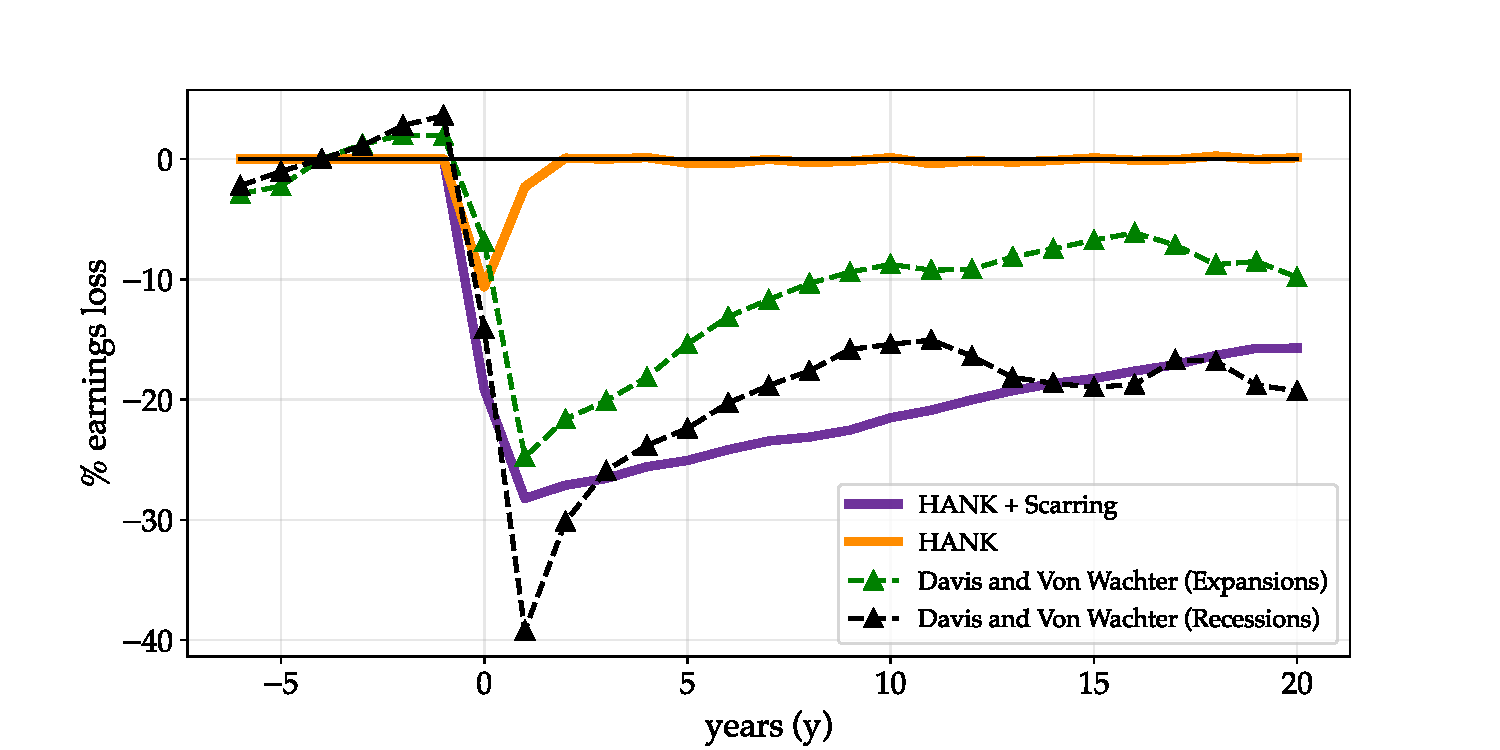
\includegraphics[scale=.65]{text/chapter1/Figures/Scarring_match}
      \caption{Earnings loss following job loss in $y=0$: Model vs Data}
 \label{Scar_match_PE}
\end{figure}
Figure \ref{Scar_match_PE}  illustrates the path of earnings loss following displacement for the baseline model with scarring (HANK + Scarring) and the model without scarring (HANK). Scarring is eliminated by assuming the probability of accumulation or erosion in human capital is eliminated. The baseline model produces a severely persistent earnings loss that is missing in the model without human capital dynamics. As in the data, these losses remain after 20 years. 




\section{Consumption Response to an Increase in Unemployment in Partial Equilibrium}

In this section, I show in partial equilibrium that the aggregate consumption response to a transitory increase in the unemployment rate is deeply persistent in the presence of scarring. I simulate the consumption response to a transitory $1\%$ increase in the unemployment rate in $t=0$. To capture the effects of scarring on consumption, I compare the simulated path of consumption in the baseline model to the simulated path of consumption to a version of the model where scarring is eliminated. I eliminate scarring by setting the probability of human capital accumulation $\pi_{L}$ and the probability of human capital erosion $\pi_{U}$ to zero. Figure \ref{Micro_results} plots the simulated path of consumption to this experiment with and without scarring. Even with $55\%$ of the increase in unemployment rate accounted for by permanent layoffs who are subject to scarring, the response of consumption is significantly more persistent than the response of the unemployment rate. 



\begin{figure}[H]
    \centering
   \begin{minipage}{0.49\textwidth}
        \centering
        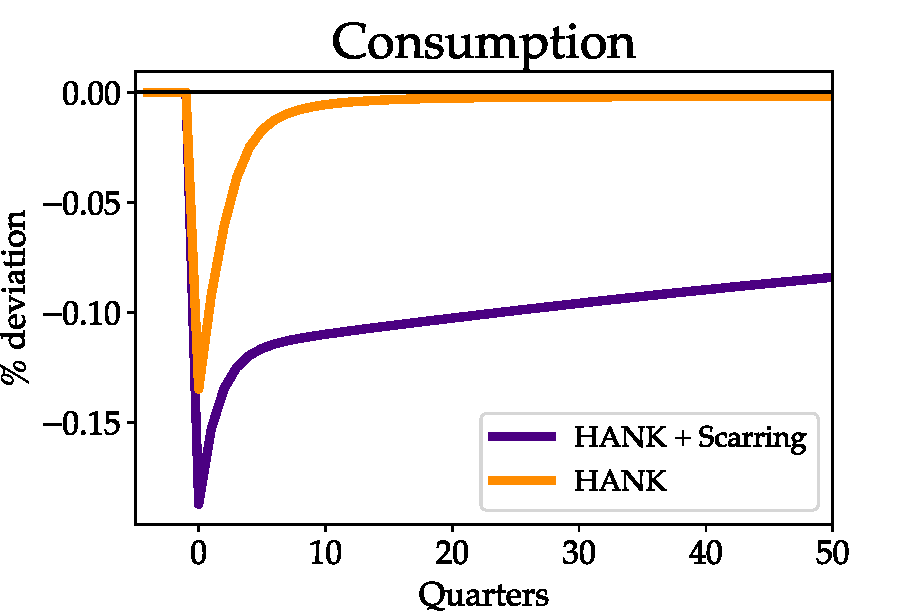
\includegraphics[width=1.1\textwidth]{text/chapter1/Figures/CJAC_JF_real_comparison} 
    \end{minipage}\hfill
    \begin{minipage}{0.49\textwidth}
        \centering
        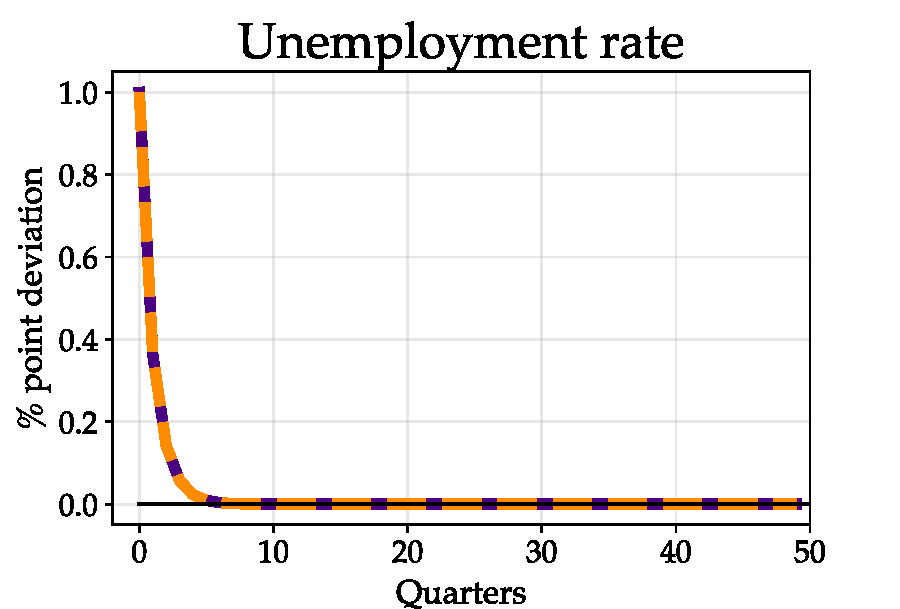
\includegraphics[width=1.1\textwidth]{text/chapter1/Figures/Urate_response_PE}
    \end{minipage}
    \caption{Consumption response to a transitory increase in the unemployment rate}
        \floatfoot{Note: The exercise above plots the consumption response to a one time negative shock to the job finding probability in $t=0$. The size of the one time shock is calibrated to increase the unemployment rate by one percentage point on impact.}
    \label{Micro_results}
\end{figure}





\section{Business Cycle Implications}


\subsection{Macroeconomic Hysteresis}

In this section, I show that unemployment scarring generates hysteresis in macroeconomic fluctuations. To illustrate this, I solve for the impulse responses to a negative demand shock, modeled as a positive discount factor shock. For simplicity, the size of the shock is the same for all ex-ante discount factor groups. The impulse responses to key aggregate variables is plotted in figure \ref{IPR_demand}. In response to this demand shock, increased patience reduces aggregate consumption leading to decreases in output and labor demand. As a result, firms post less vacancies lowering the job finding probability and raising the unemployment rate. As households lose their jobs, on average, they find jobs at a lower wage leading to persistent losses in mean human capital. This causes consumption, output, and labor income to exhibit hysteresis while the unemployment rate recovers with the demand shock. Notably, the responses to consumption, output, debt, and mean human capital still do not recover after 100 quarters, long after the recovery in the unemployment rate. Since unemployment does not exhibit hysteresis, wages nor the vacancy filling rate will either. As a result marginal costs, and therefore inflation, do not exhibit any persistence. 


\begin{figure}[!h]
    \centering % <-- added
\begin{minipage}{0.33\textwidth}
  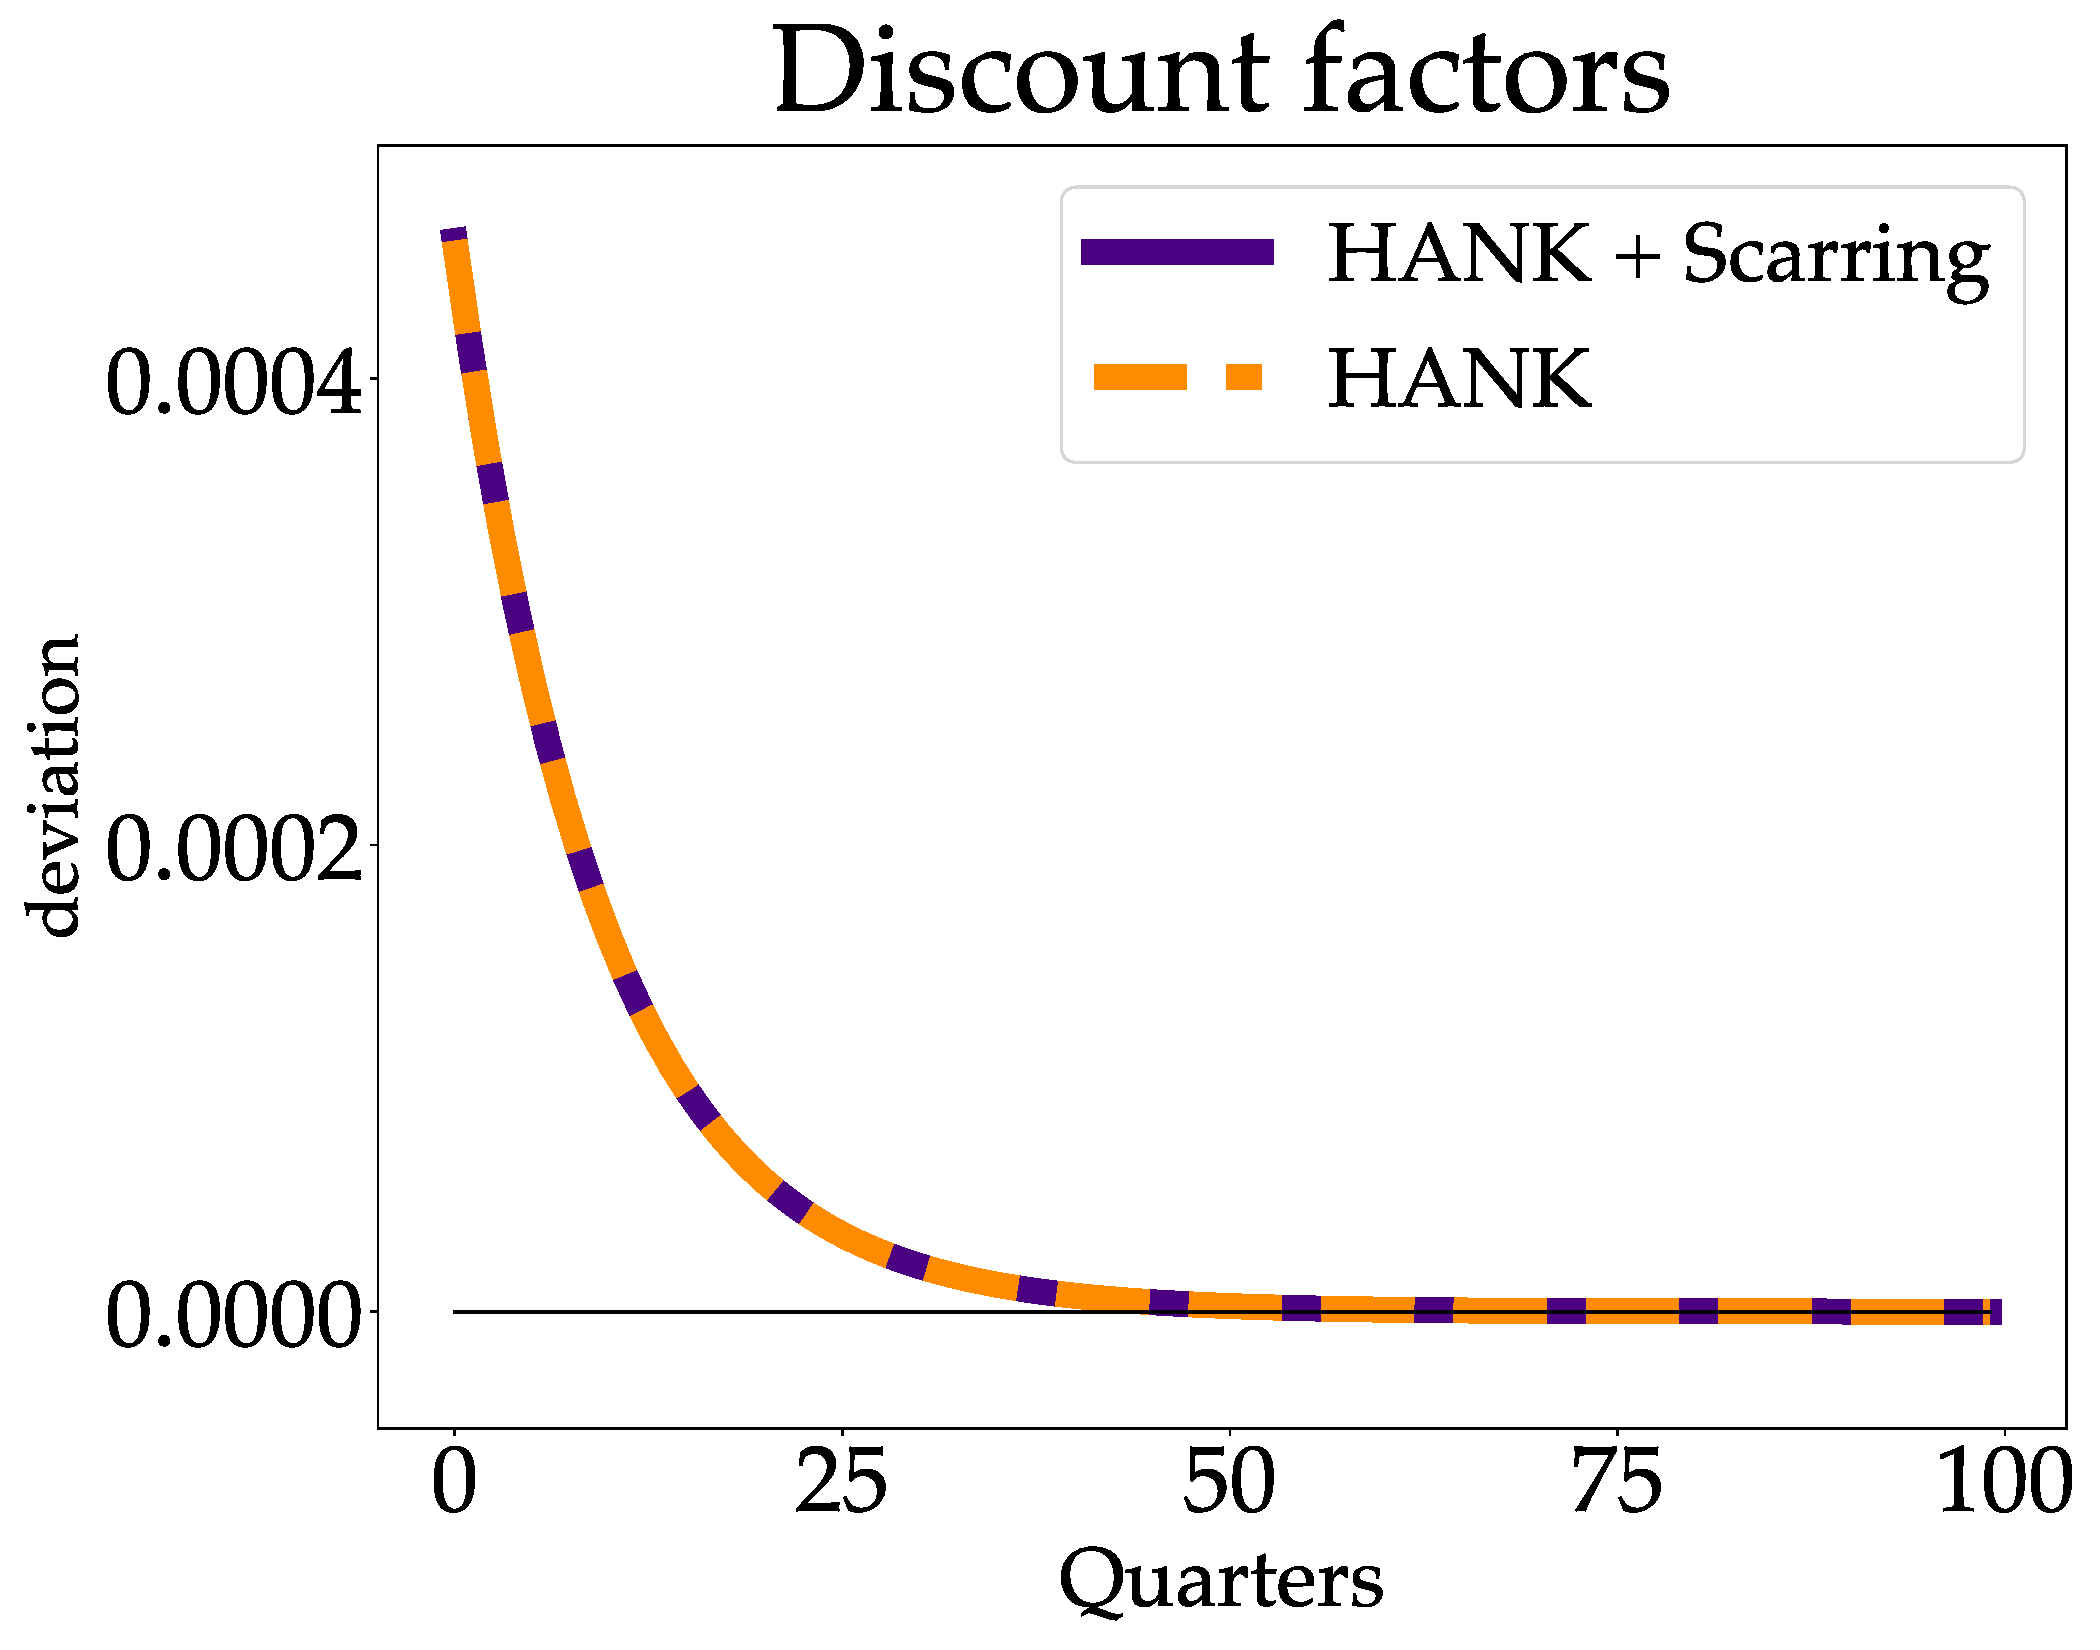
\includegraphics[scale=.14]{text/chapter1/Figures/DiscFac_IPR}
  \label{fig:1}
\end{minipage}\hfil % <-- added
\begin{minipage}{0.33\textwidth}
  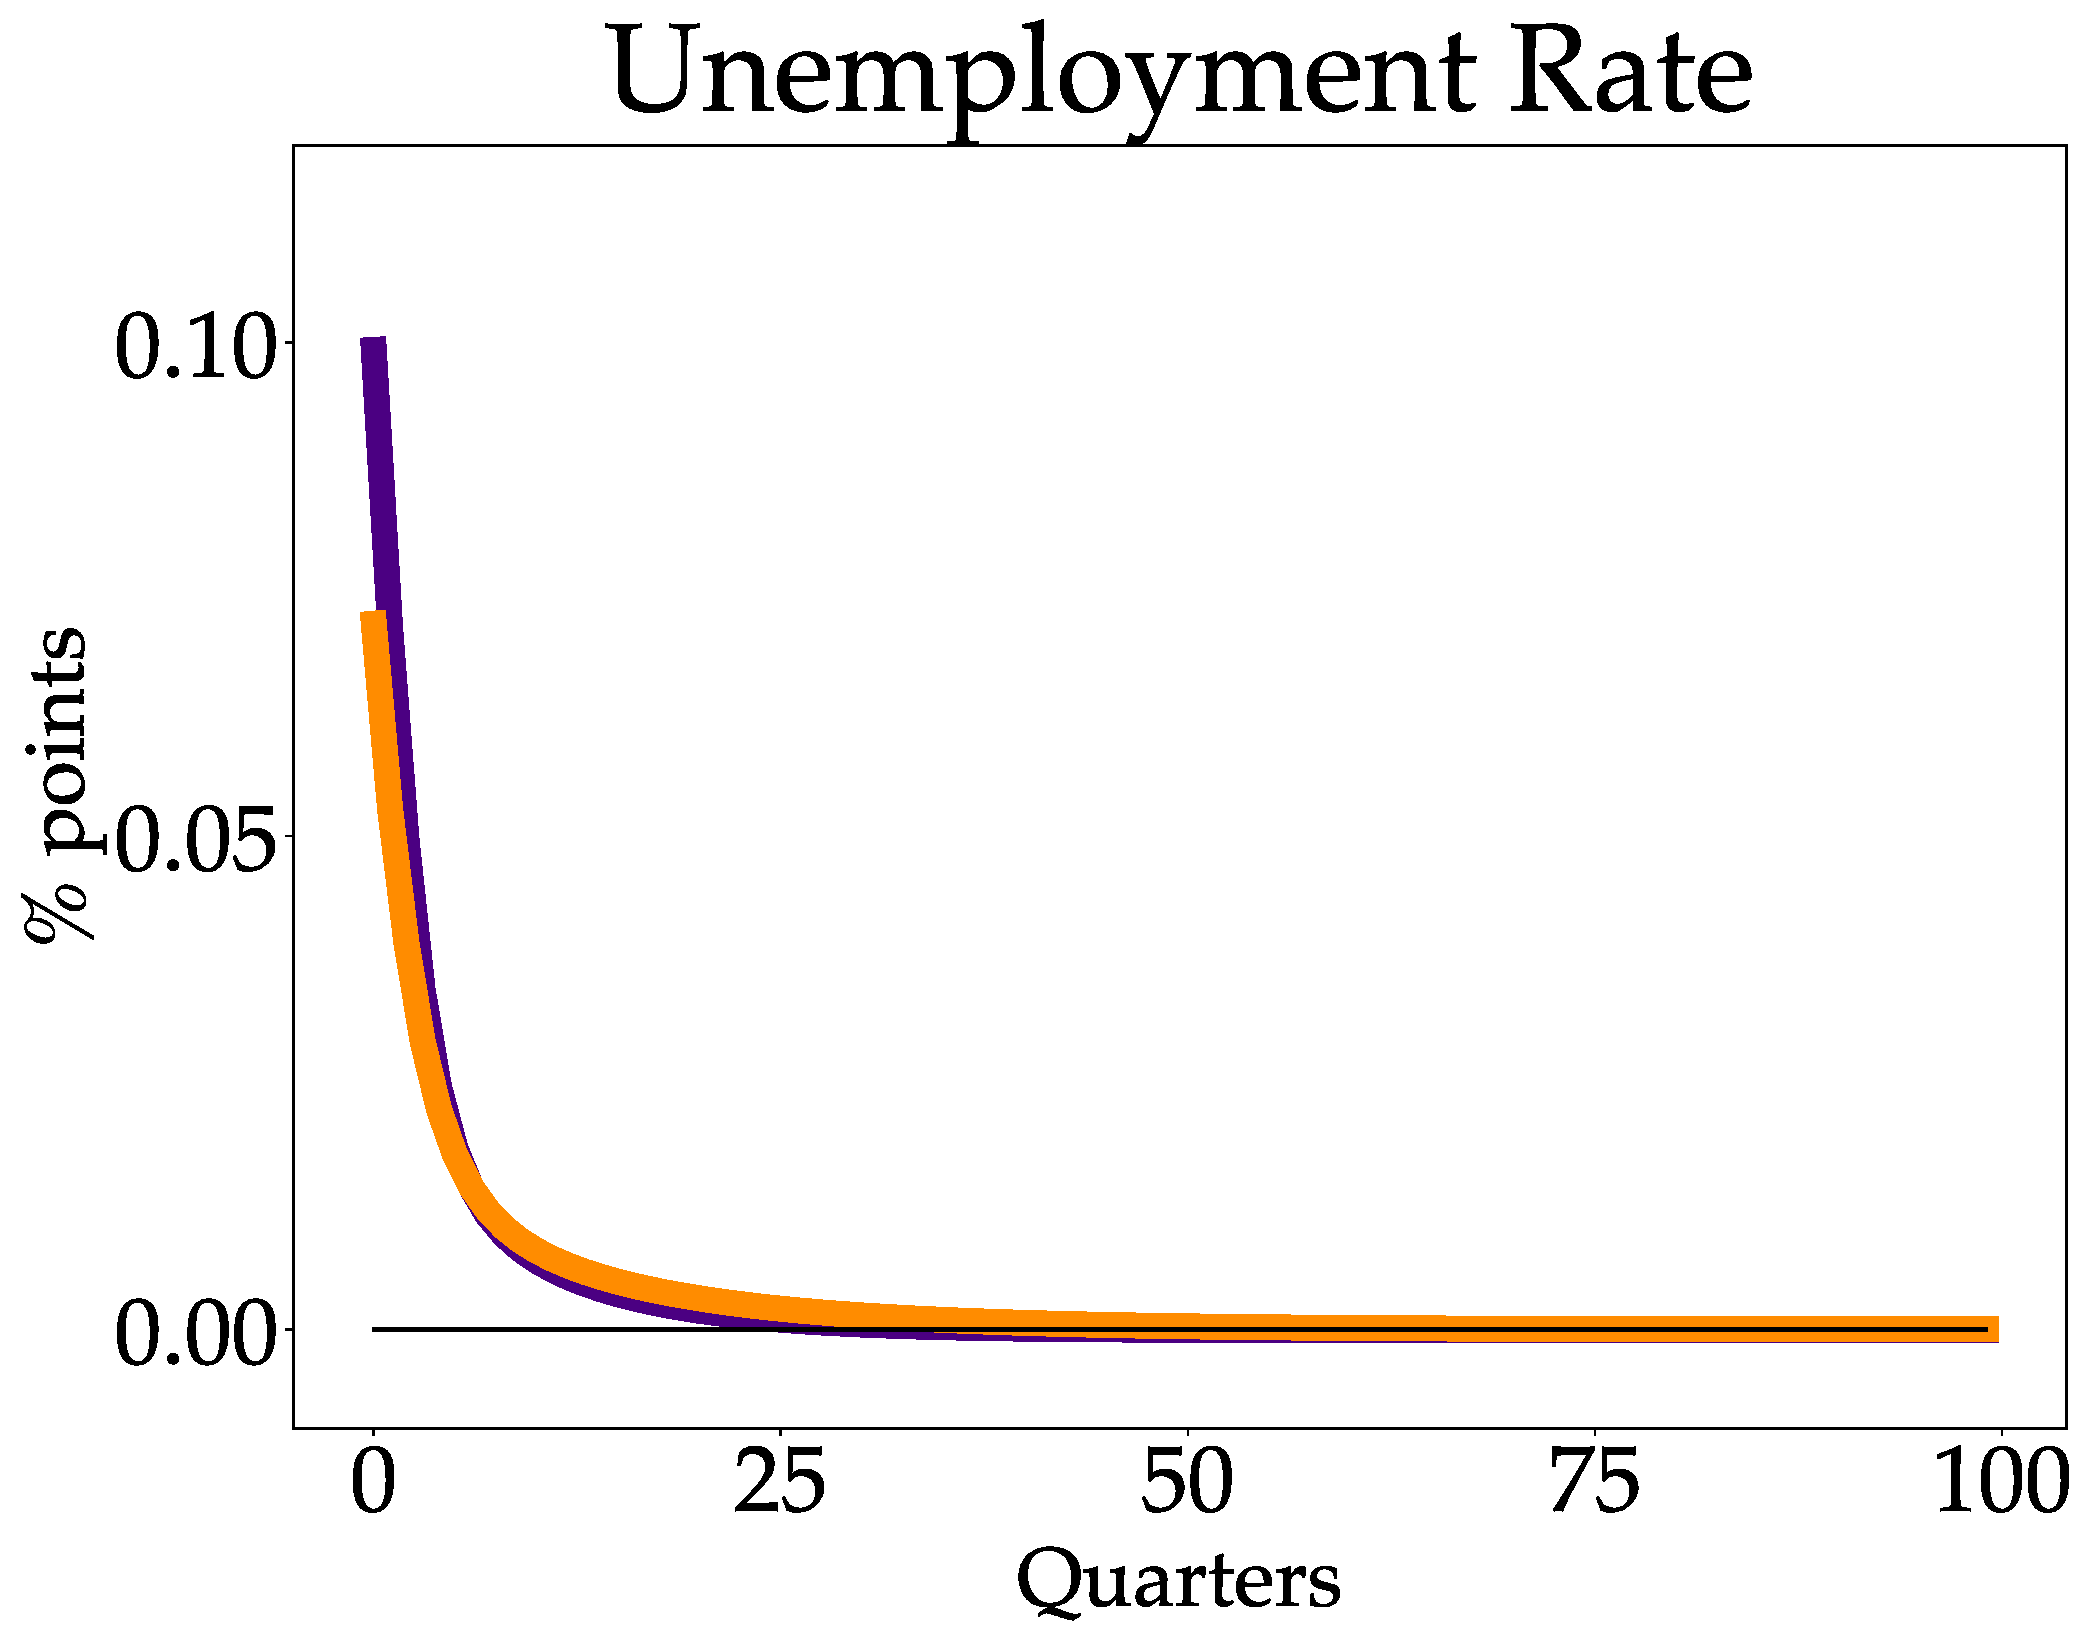
\includegraphics[scale=.14]{text/chapter1/Figures/U_IPR}
  \label{fig:2}
\end{minipage}\hfil % <-- added
\begin{minipage}{0.33\textwidth}
  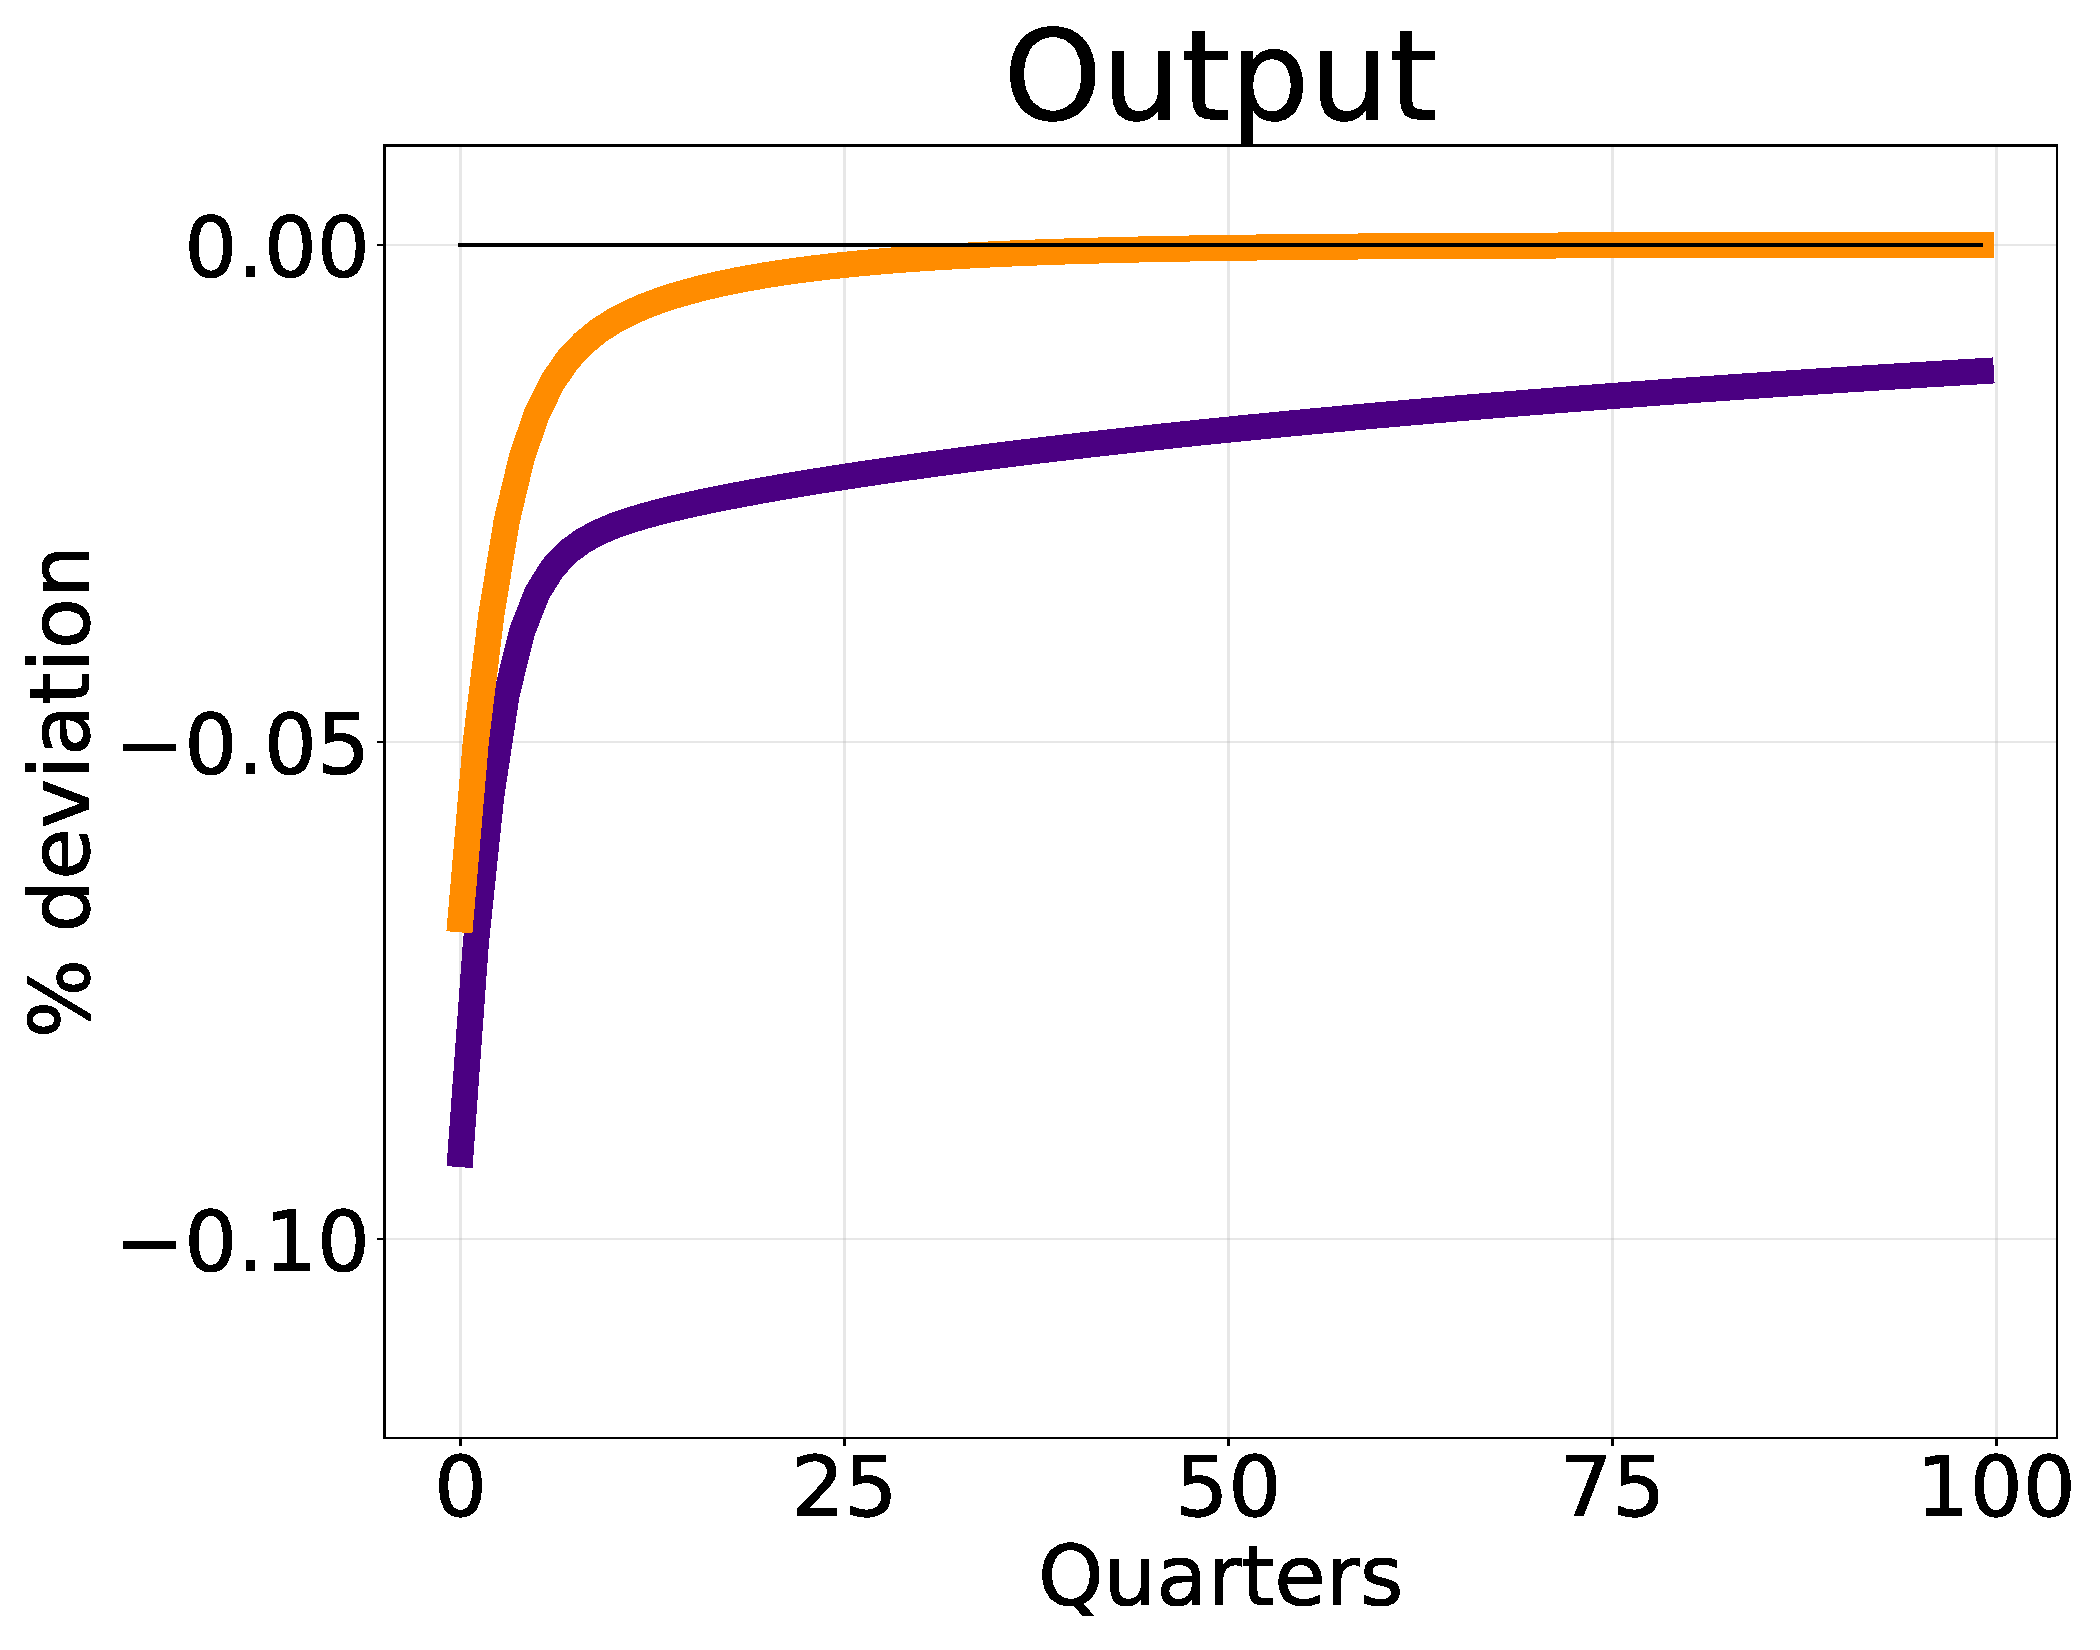
\includegraphics[scale=.14]{text/chapter1/Figures/Y_IPR}
  \label{fig:3}
\end{minipage}
\begin{minipage}{0.33\textwidth}
  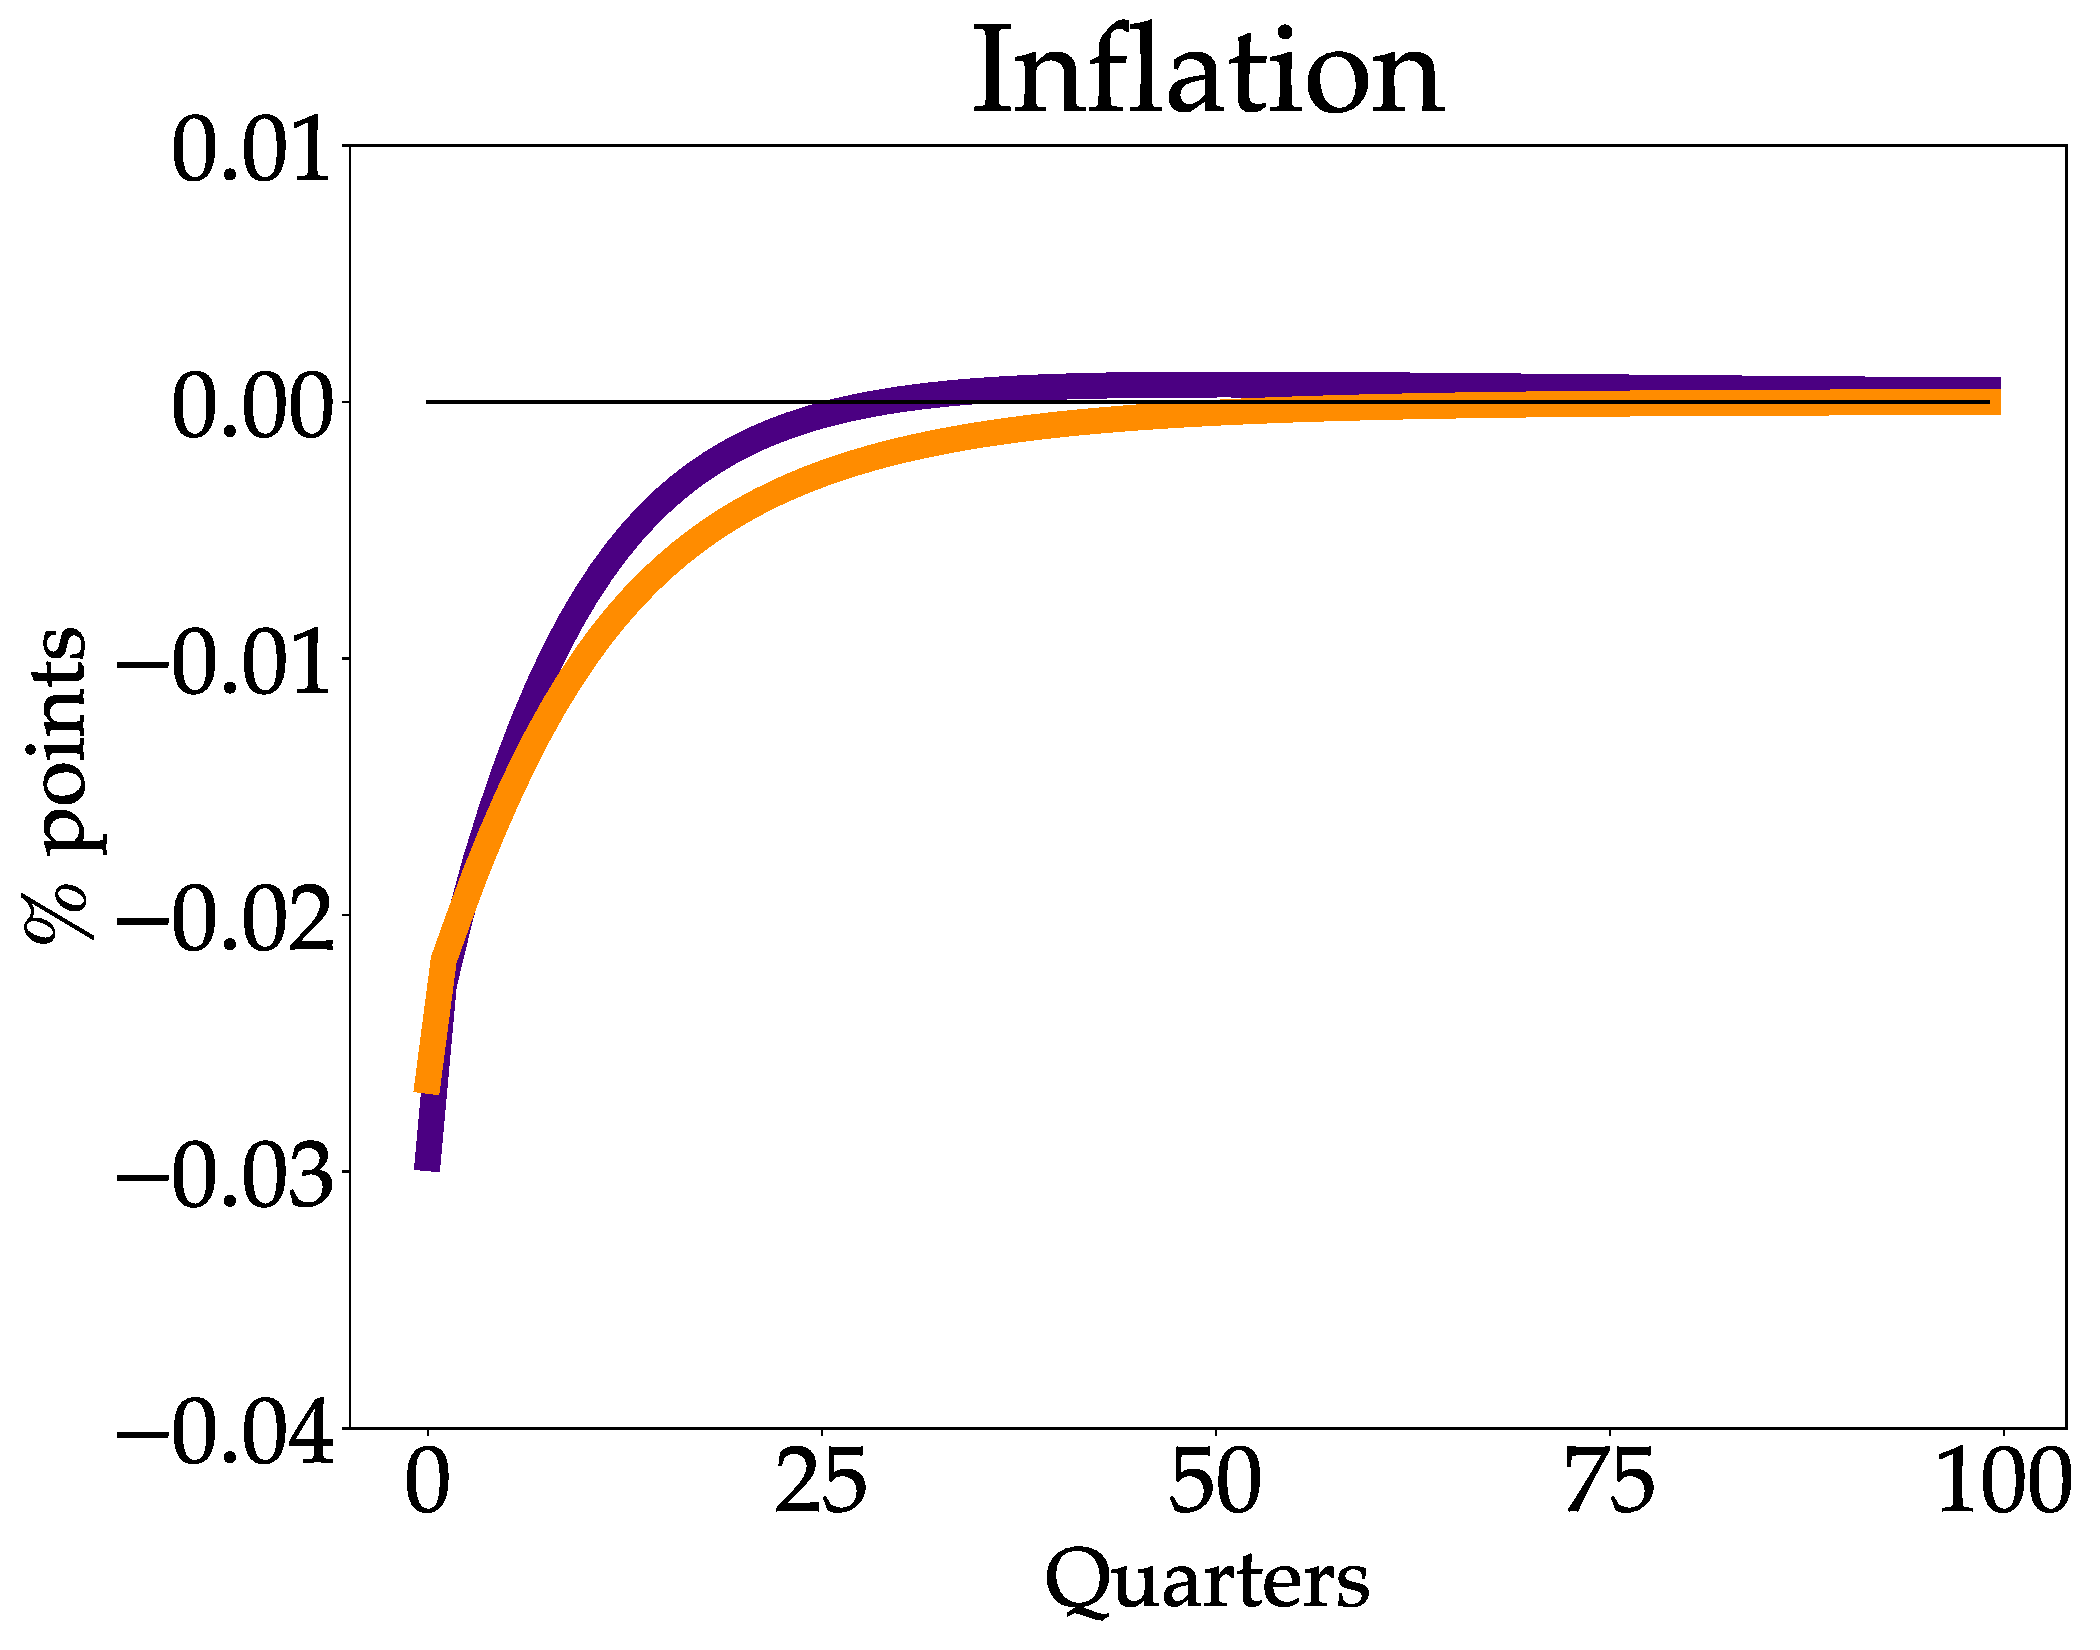
\includegraphics[scale=.14]{text/chapter1/Figures/pi_IPR}
  \label{fig:4}
\end{minipage}
\medskip
\begin{minipage}{0.33\textwidth}
  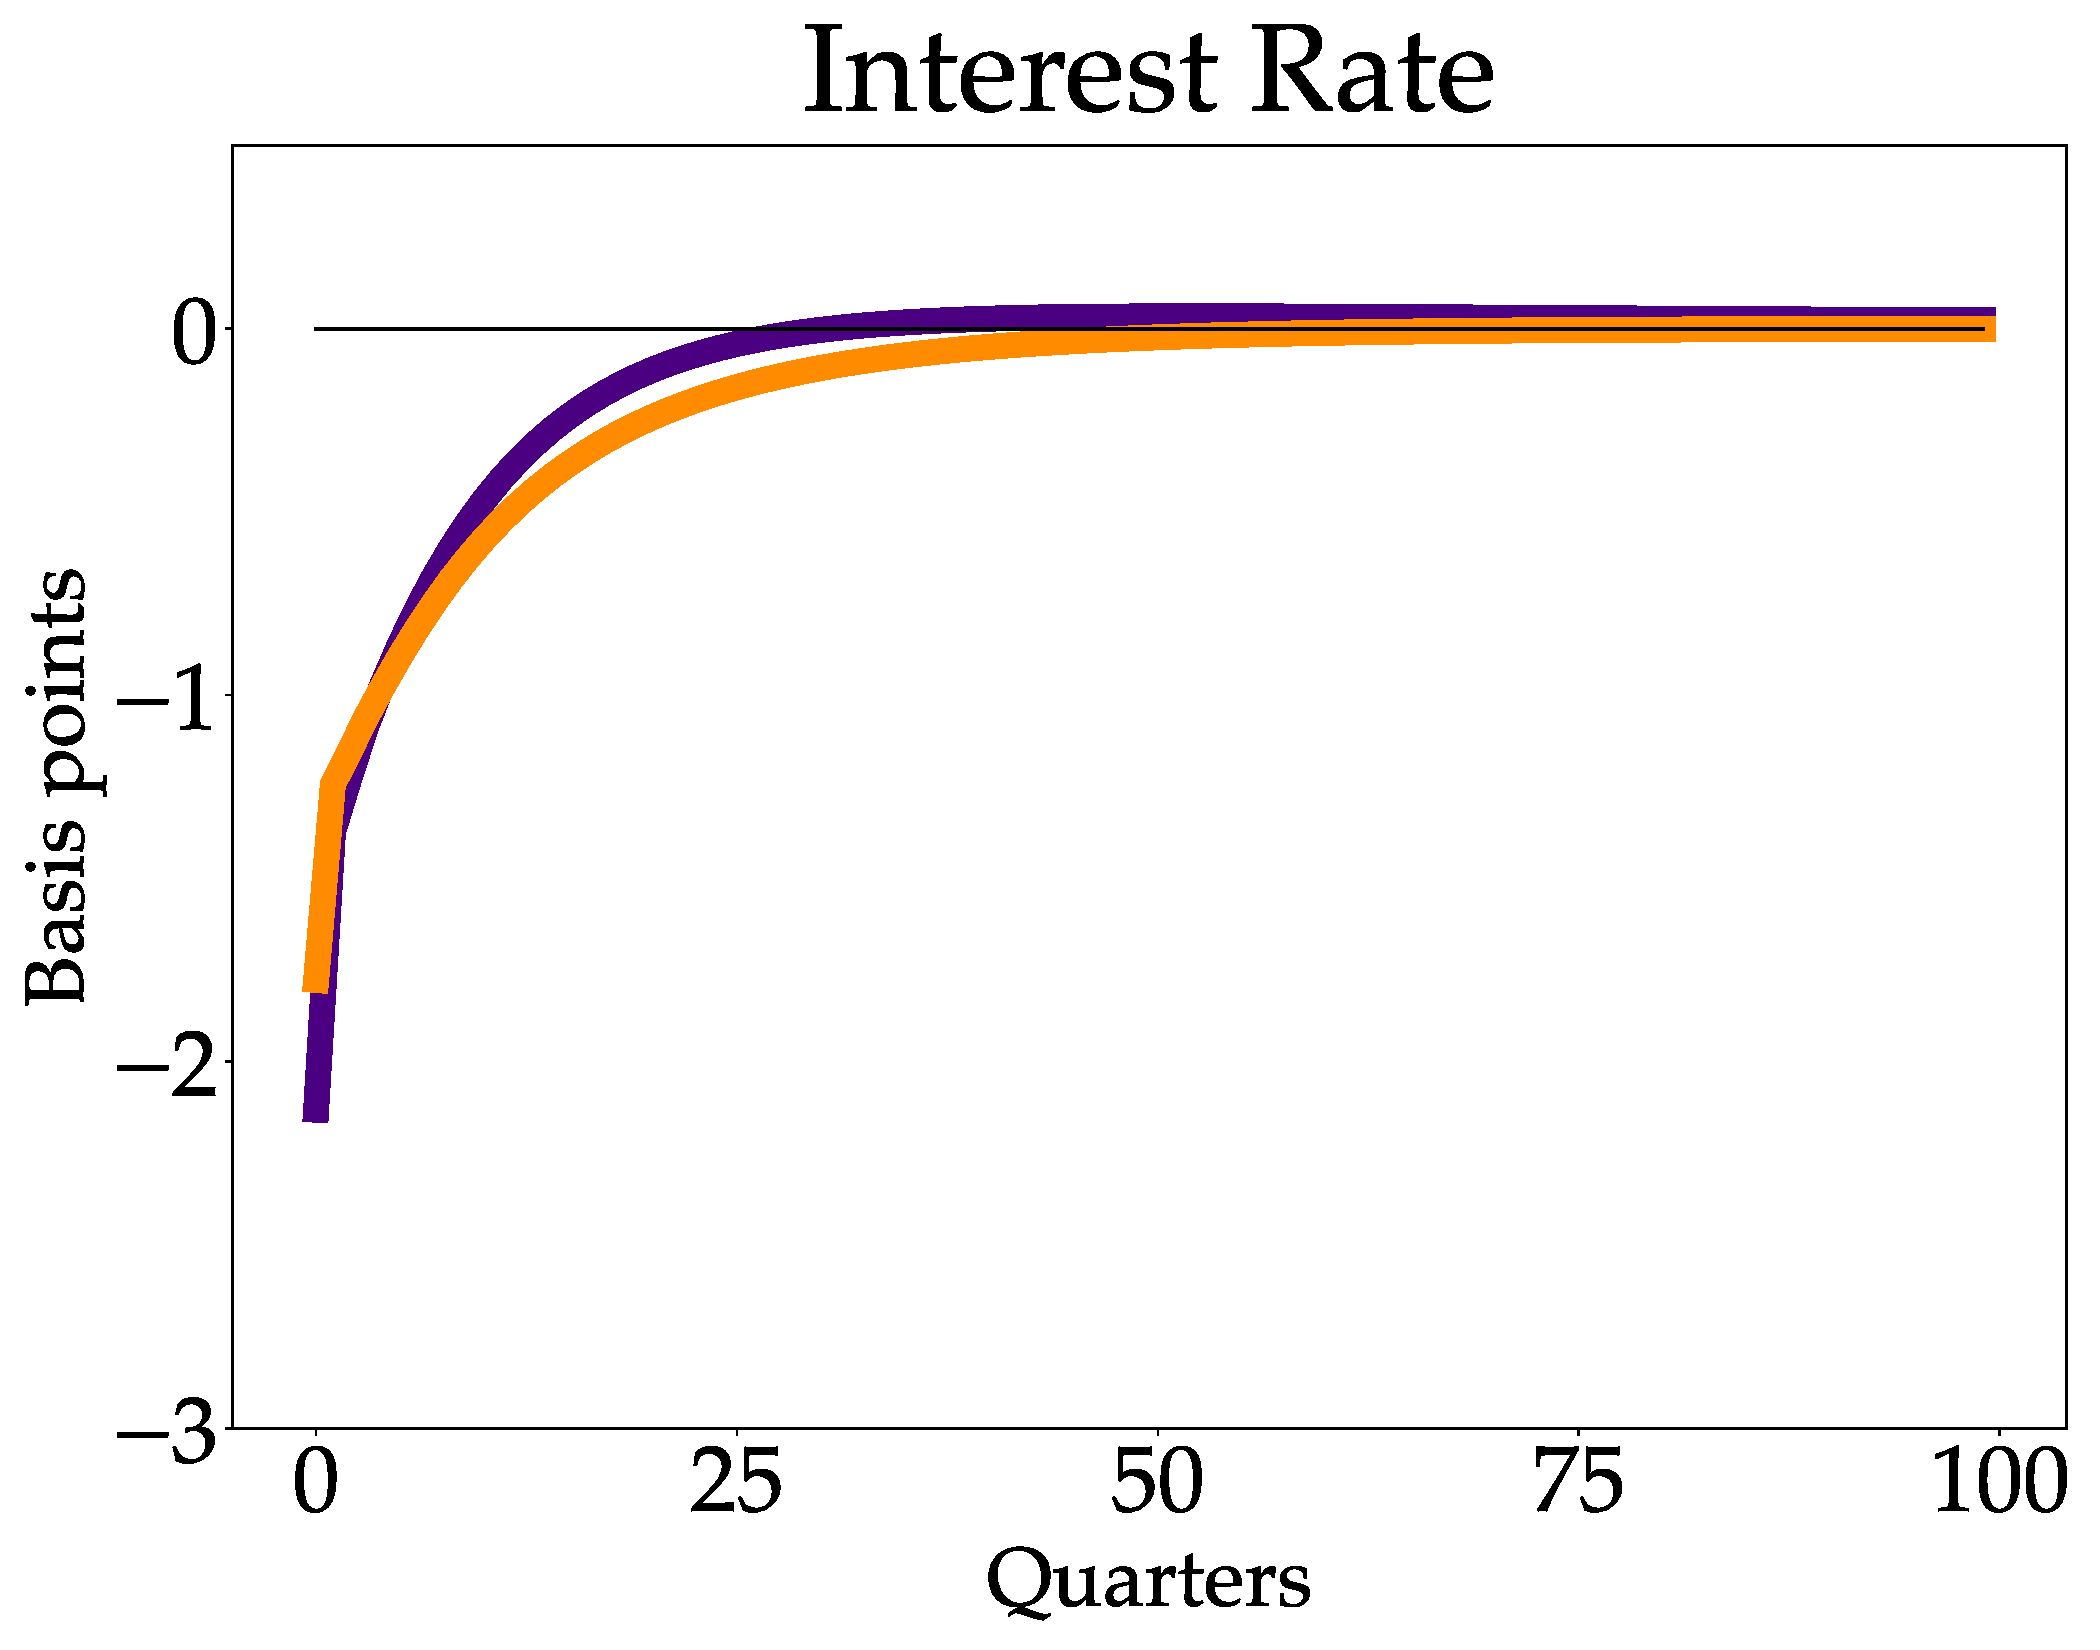
\includegraphics[scale=.14]{text/chapter1/Figures/r_IPR}
  \label{fig:4}
\end{minipage}\hfil % <-- added
\begin{minipage}{0.33\textwidth}
  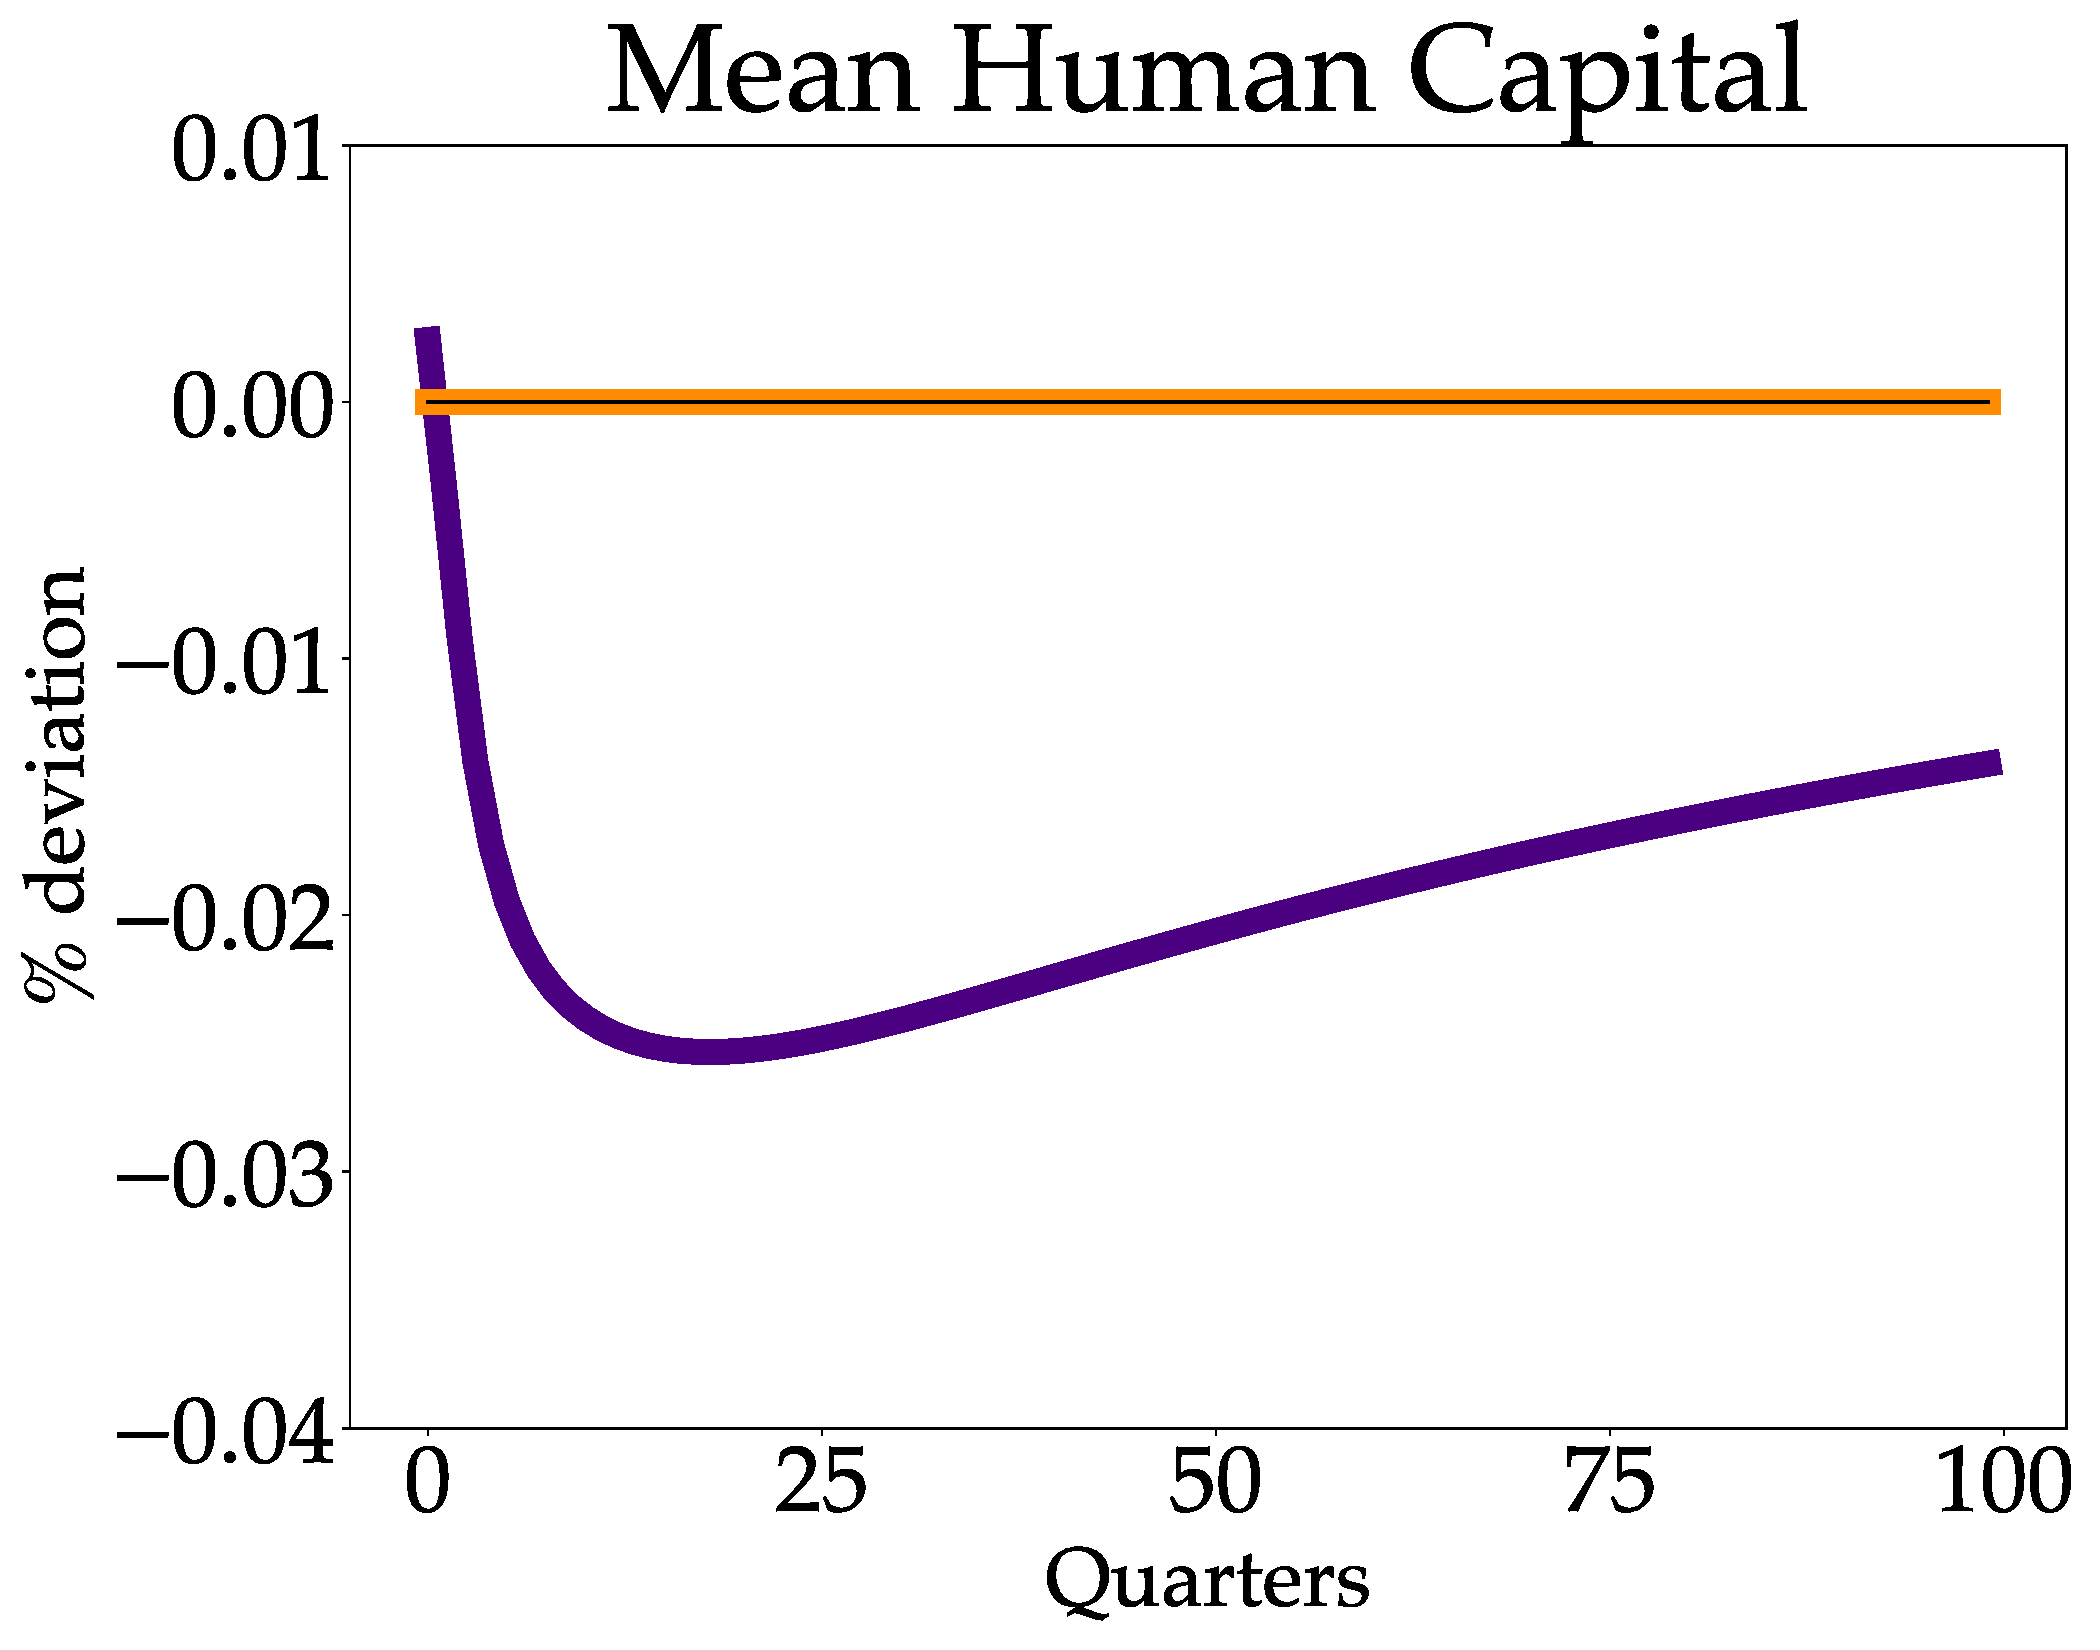
\includegraphics[scale=.14]{text/chapter1/Figures/H_E_IPR}
  \label{fig:5}
\end{minipage}\hfil % <-- added
\caption{Impulse responses to a negative demand shock} 
\floatfoot{Note: The exercise above plots the impulse responses to a positive discount factor shock. The quarterly persistence of the shock is $0.9$ and the size of the shock is then calibrated to generate a 0.1 percentage point increase in the unemployment rate.}
\label{IPR_demand}
\end{figure}


\subsection{Unemployment Scarring and Inequality}

With unemployment scarring, an increase in unemployment leads to a persistent rise in income inequality. Figure \ref{Gini_IPR} plots the impulse response of the labor income gini index across households to the negative demand shock under the baseline model and under the model without scarring. In the baseline model, the initial increase in the gini index is attributed to the rise in unemployment and the decline in the aggregate wage. The persistence of the gini index response is due to the recomposition of the distribution of human capital of employed households. In particular, as unemployed households find reemployment at lower levels of human capital. Since the human capital of newly employed households accumulates slowly, this causes hysteresis in the gini index. In the model without scarring, the increase in income inequality is transitory as it is only affected by transitory changes in the unemployment rate and the aggregate wage.

\begin{figure}[!h]
   \begin{center}
   \begin{minipage}{0.7\textwidth}
        \centering
        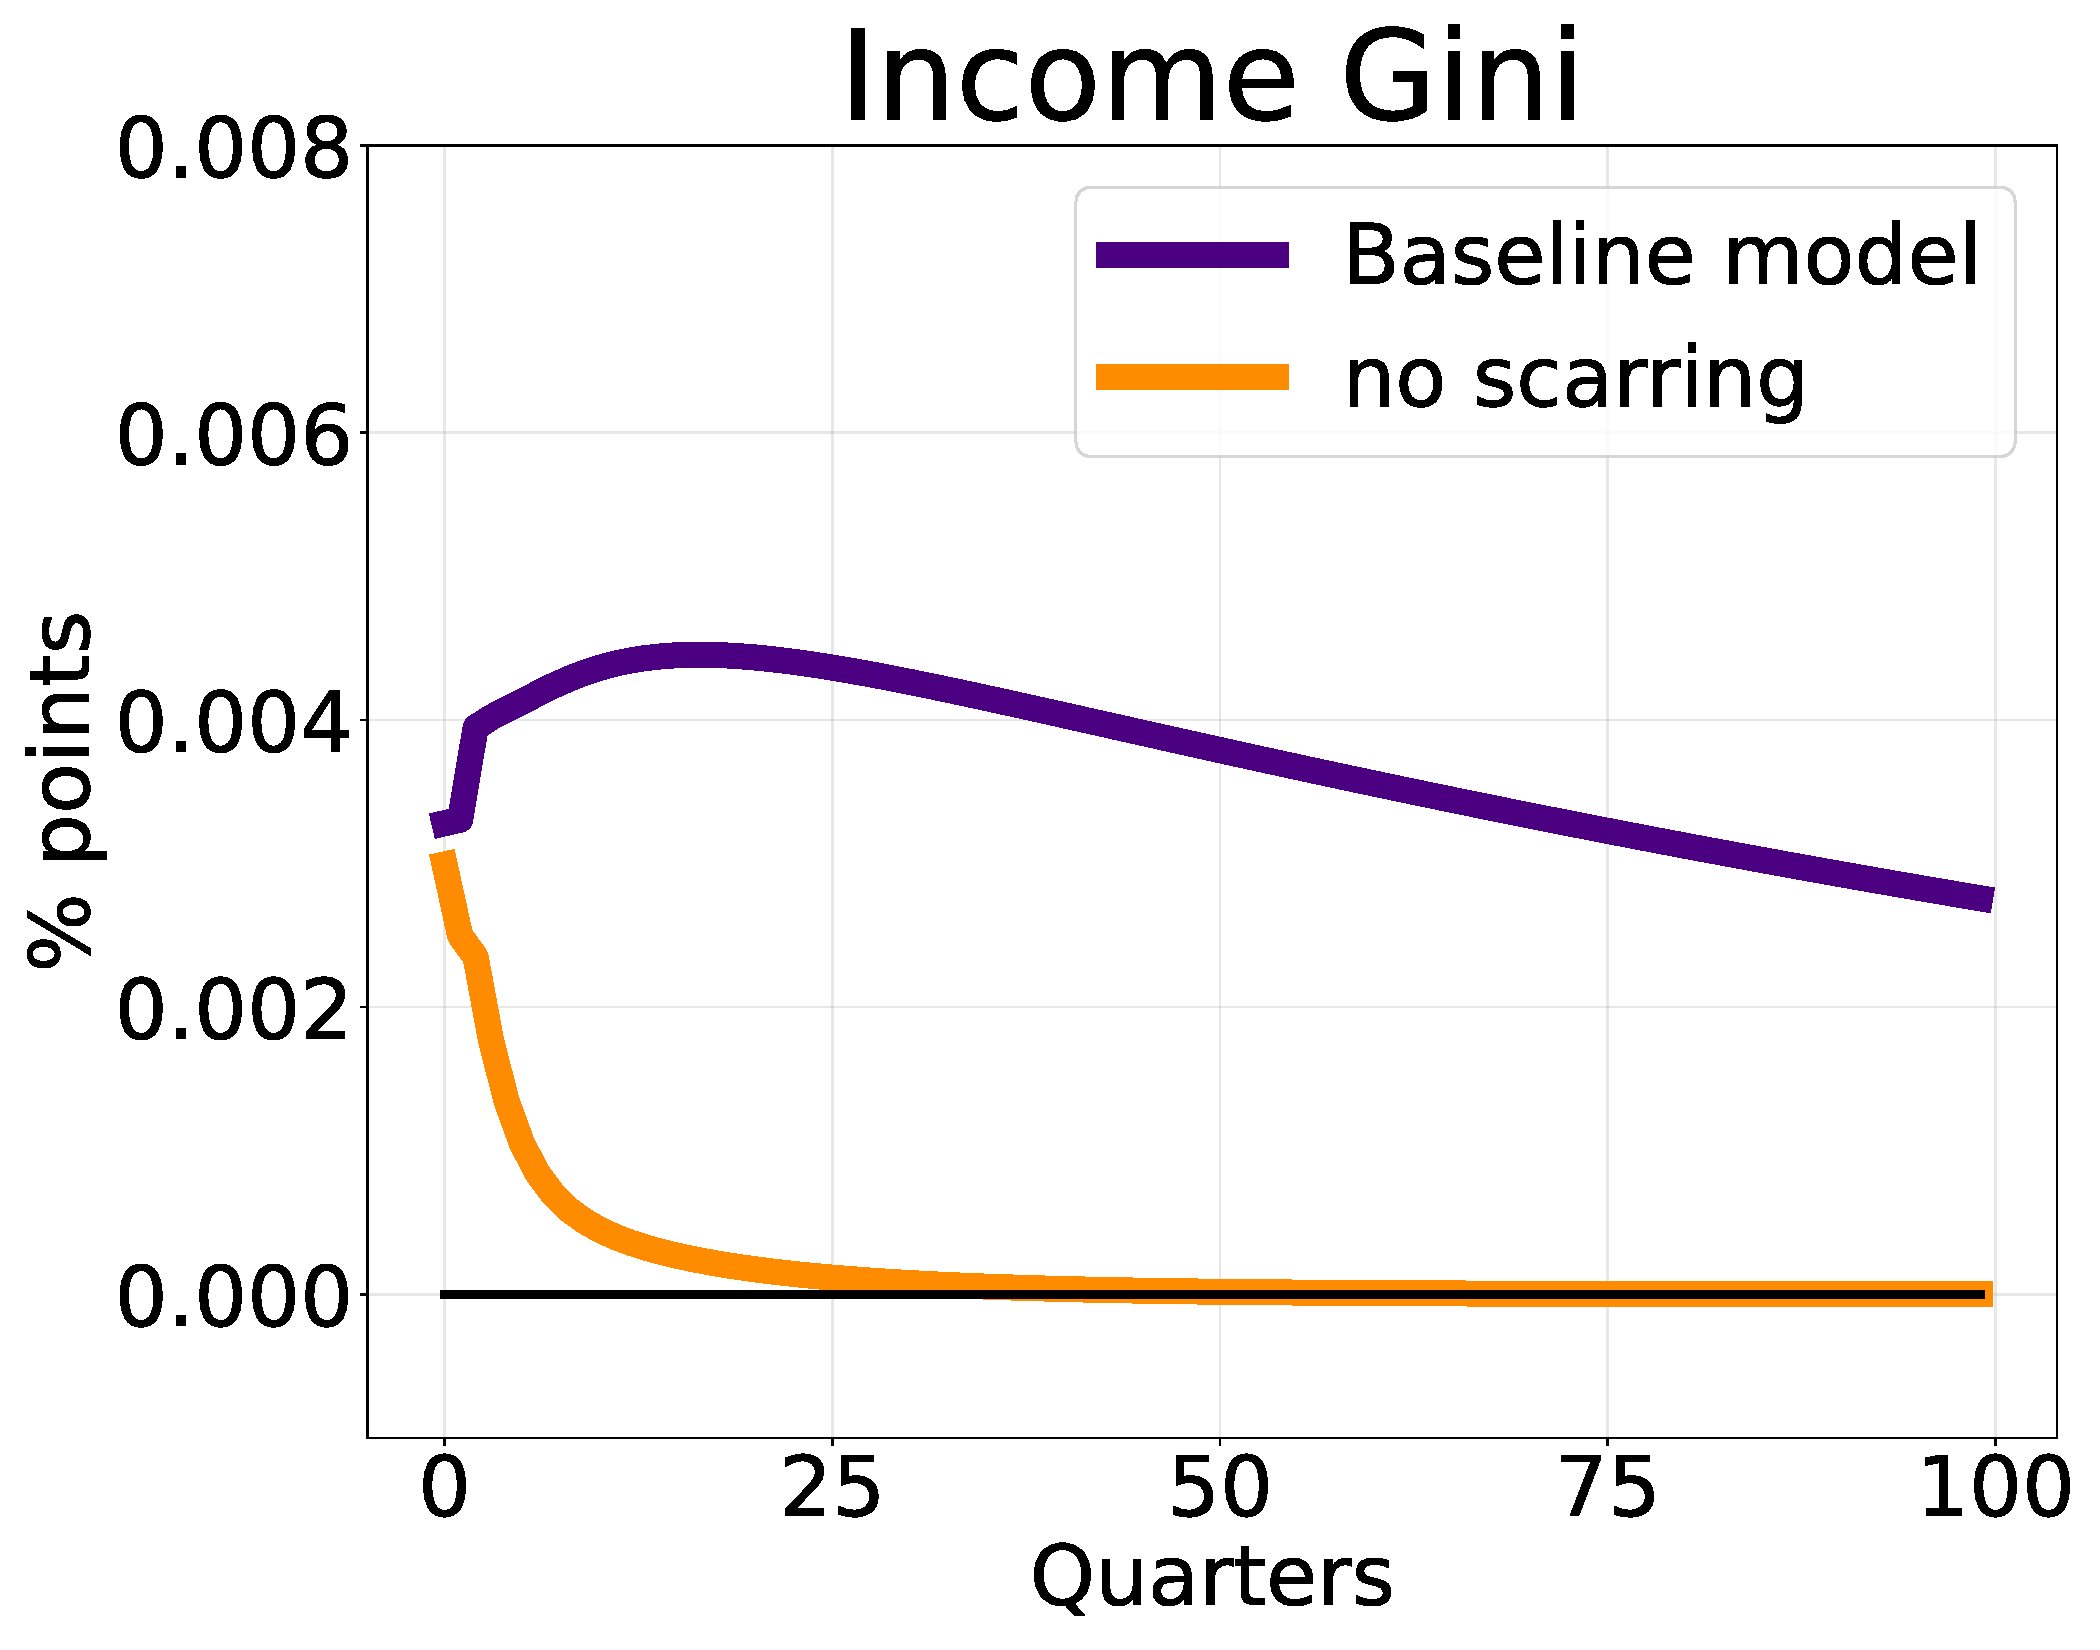
\includegraphics[scale=.3]{text/chapter1/Figures/gini_IPR} % first figure itself
    \end{minipage}
        \caption{Response of income Gini index to negative demand shock.}
        \floatfoot{Note: This exercise plots the impulse response of the Gini index from the negative demand shock in \ref{IPR_demand}.}
    \label{Gini_IPR}
    \end{center}
  \end{figure}




\subsection{Scarring and Debt to GDP}

Unemployment scarring increases the pressure that recessions place on national debt. Figure \ref{debt_to_GDP} plots the responses of debt to GDP and debt to the demand shock from previous section. The figure demonstrates that the debt to GDP and debt increase much more persistently in the presence of scarring. This is due to the pressure that scarring places on tax revenues. As households lose their jobs and find reemployment at a lower effective wage, the tax base is scarred. This persistent decline in tax revenues require the government to borrow substantially more to maintain their expenditures.


\begin{figure}[!h]
    \centering
   \begin{minipage}{0.47\textwidth}
        \centering
        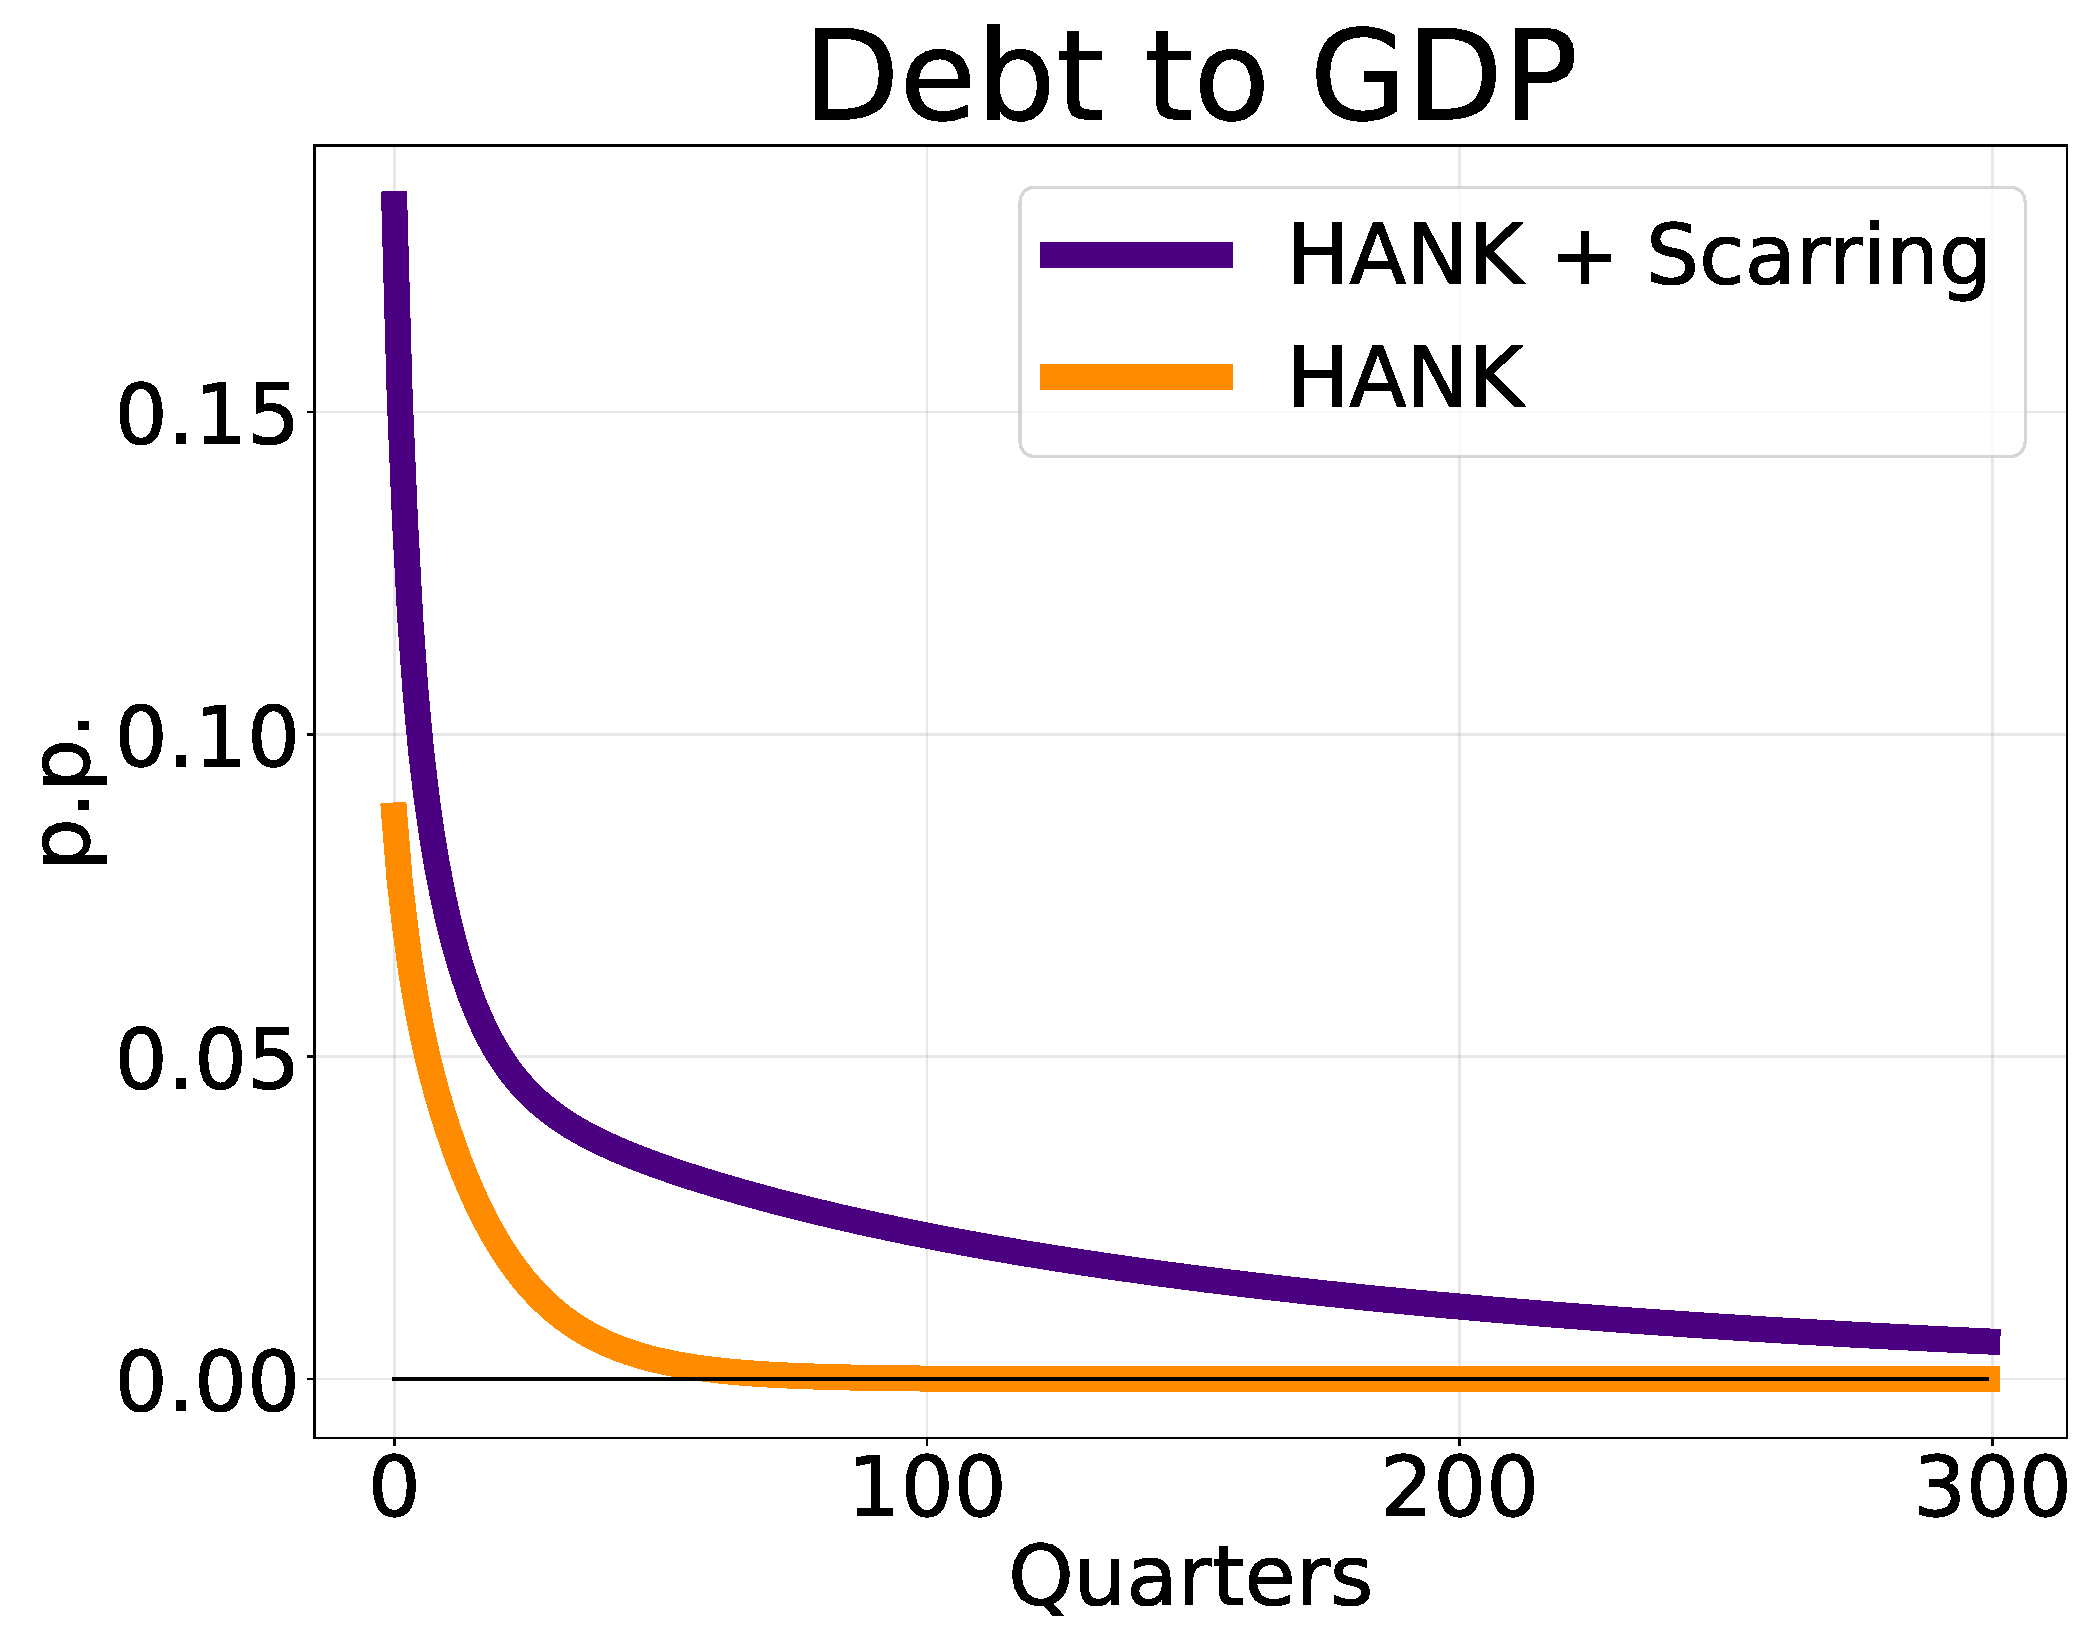
\includegraphics[scale=.2]{text/chapter1/Figures/debt_to_GDP_IPR} % first figure itself
    \end{minipage}\hfill
    \begin{minipage}{0.47\textwidth}
        \centering
        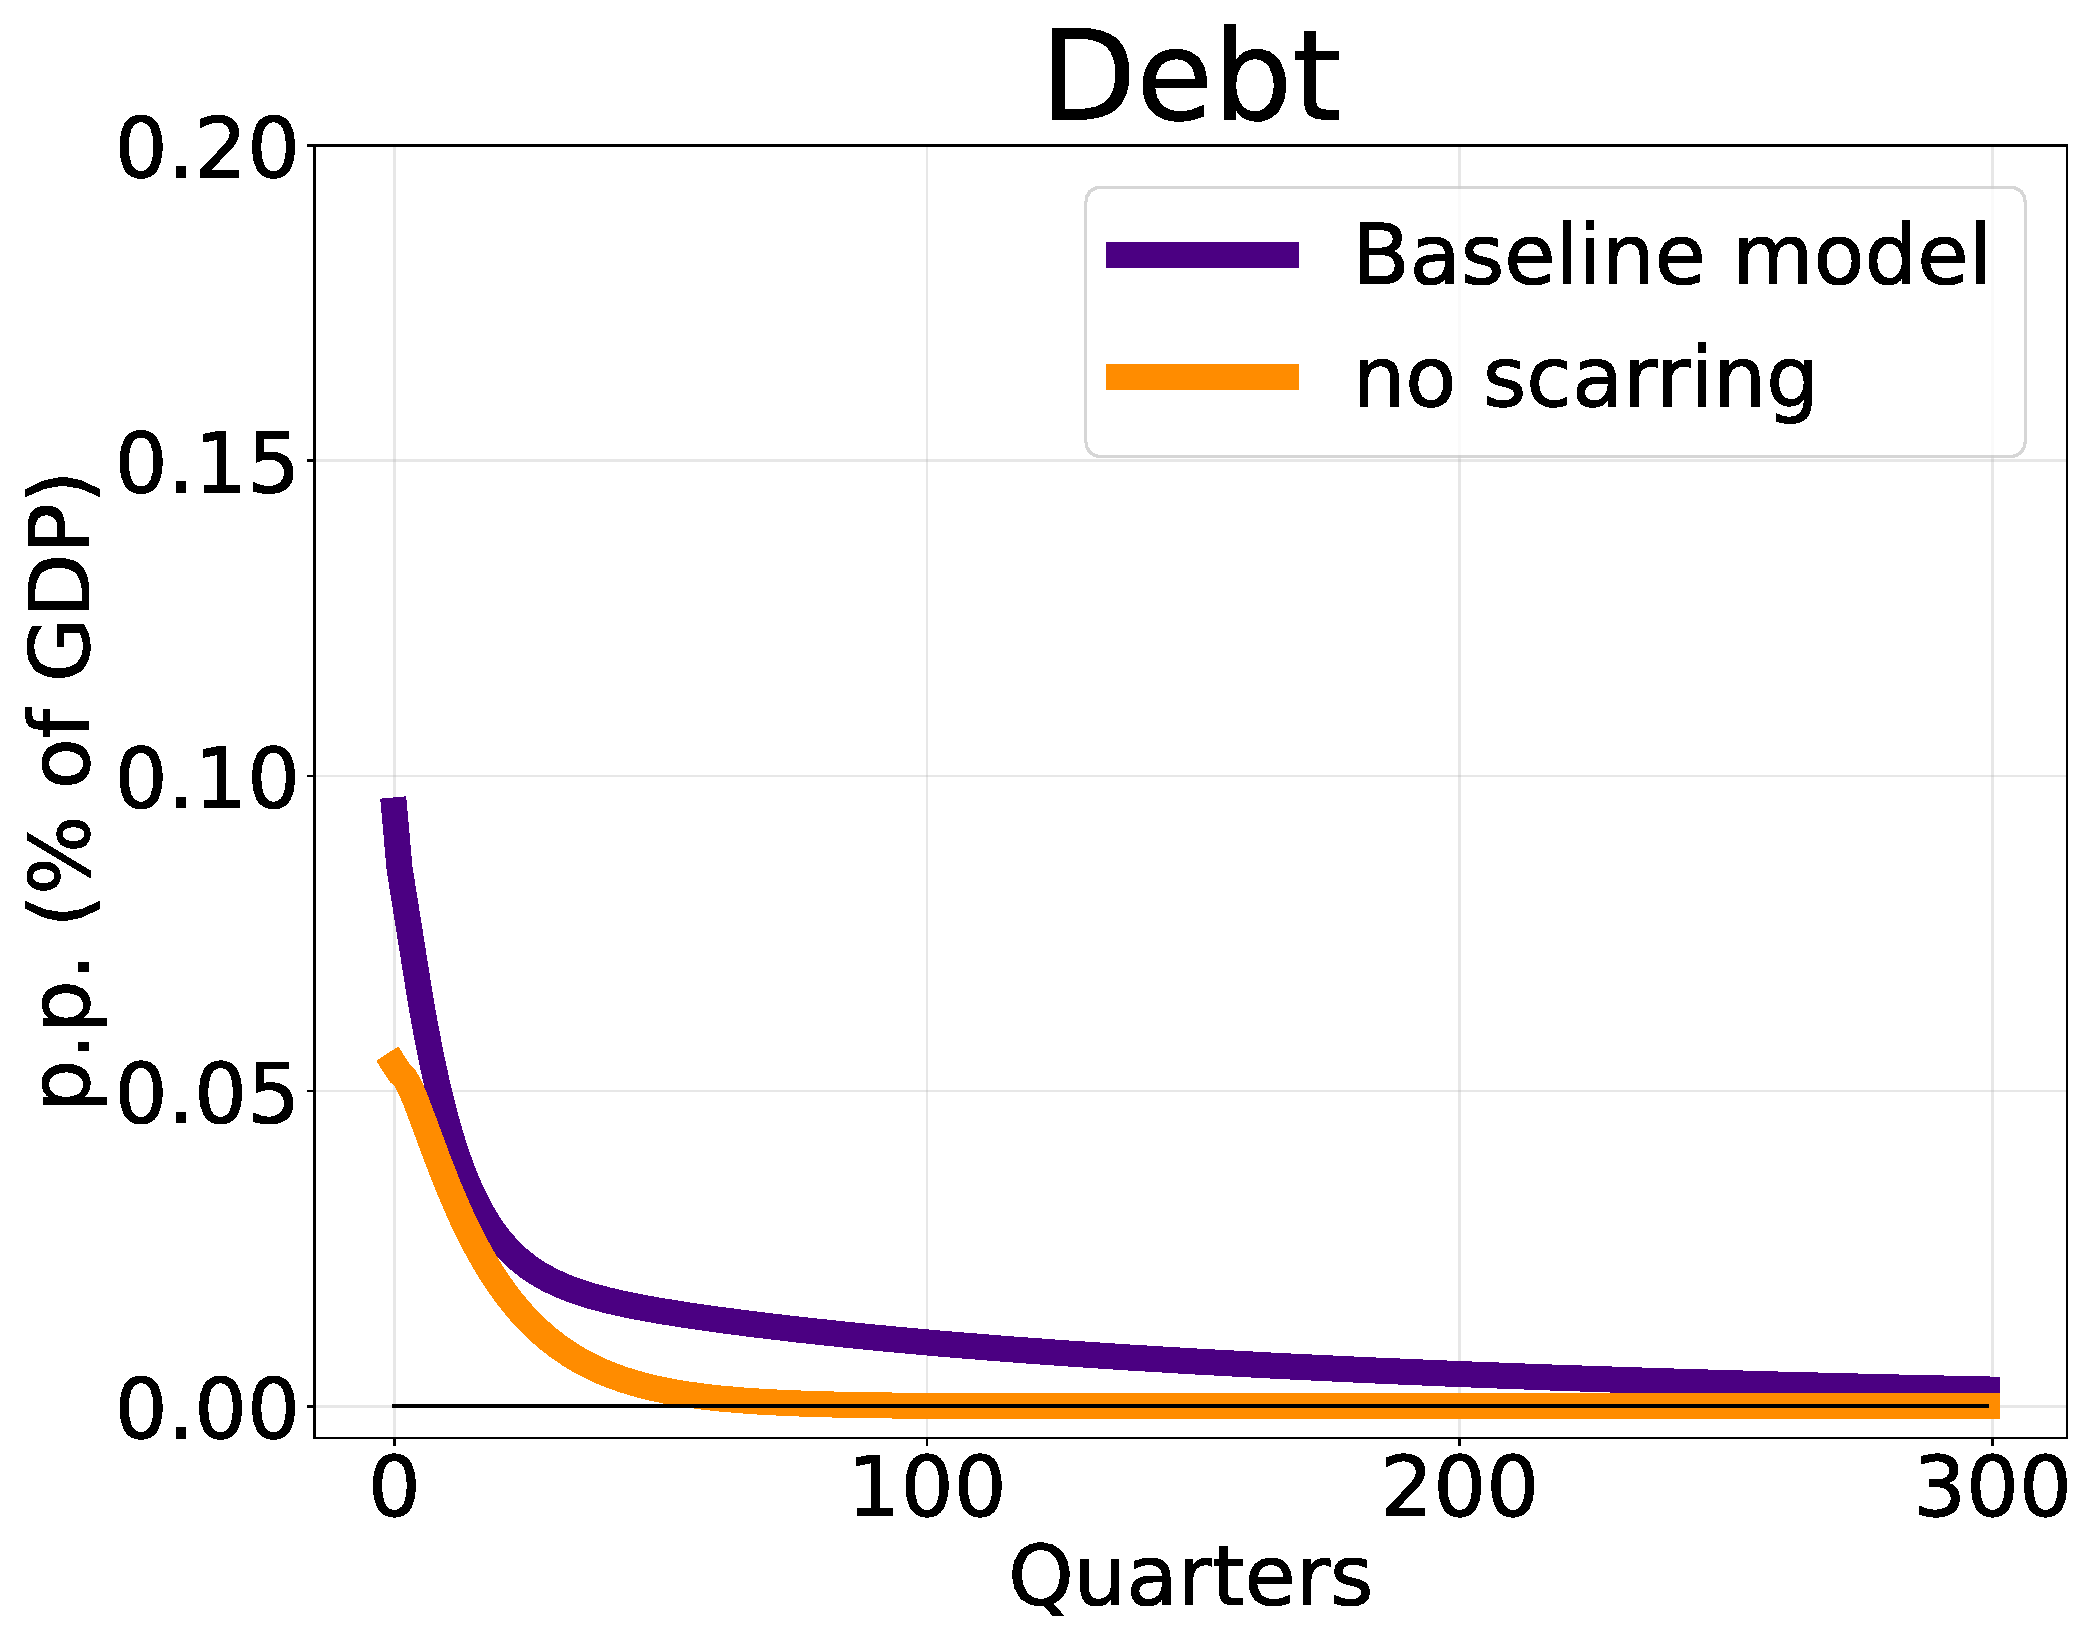
\includegraphics[scale=.2]{text/chapter1/Figures/debt_IPR} % second figure itself
    \end{minipage}
    \caption{Responses of debt and debt to GDP to negative demand shock}
     \floatfoot{Note: This exercise plots response of the debt-to-GDP and debt from the negative demand shock in \ref{IPR_demand}.}
    \label{debt_to_GDP}
\end{figure}


\section{Scarring and the Transmission of Fiscal Policy}

Having established that in the presence of unemployment scarring, aggregate shocks lead to persistent responses in output. In this section, I show that fiscal multipliers are substantially larger and rise with the horizon because of unemployment scarring. To do so, I consider a negative government spending shock in the baseline model and the model without scarring and compute the multipliers across the horizon. In particular the multiplier is defined as:



$$ \text{Multiplier} = \frac{\Sigma_{t=0}^{H}  \frac{1}{R^{t}}\Delta Y_{t}}{ \Sigma_{t=0}^{H}  \frac{1}{R^{t}}\Delta{G_{t}}}$$ 

where $H$ is the horizon of the mulitplier. \\

Figure \ref{Fiscal_multipliers} plots the fiscal multipliers to a contractionary government spending shock across the horizon of the multiplier under the baseline model and model without scarring.


\begin{figure}[!h]
    \centering
   \begin{minipage}{0.68\textwidth}
        \centering
        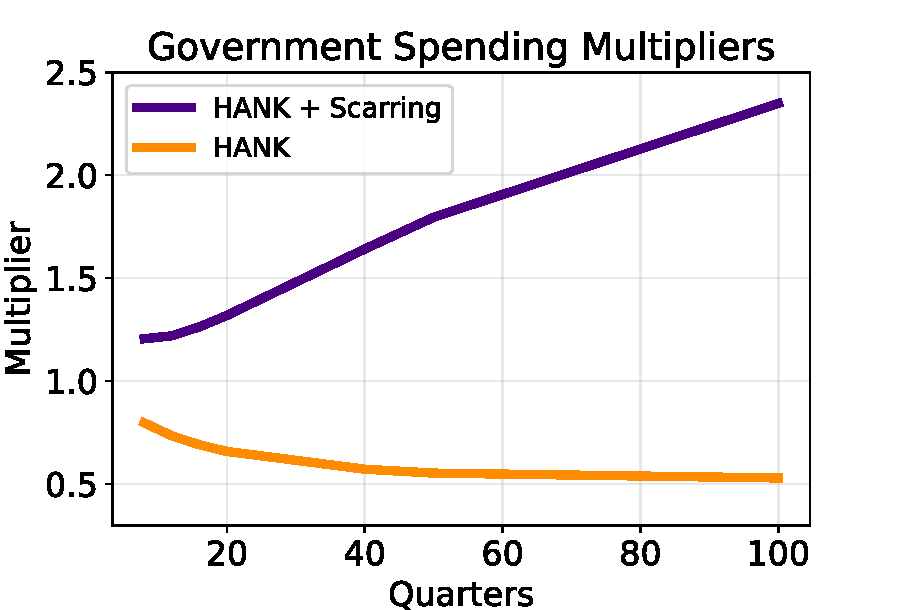
\includegraphics[scale=.7]{text/chapter1/Figures/multipliers} % first figure itself
    \end{minipage}
        \caption{Fiscal Multipliers to a negative government spending shock.}
    \label{Fiscal_multipliers}
    \floatfoot{Note: This figure plots the multiplier out of negative government spending shock with a quarterly AR(1) persistence of 0.933 across the horizon $H$ of the multiplier. For example, a point on the purple line at quarters = 20 represents the fiscal multiplier: $ \frac{\Sigma_{t=0}^{20}  \frac{1}{R^{t}}\Delta Y_{t}}{ \Sigma_{t=0}^{20}  \frac{1}{R^{t}}\Delta{G_{t}}}$. }
\end{figure}


The multipliers under the baseline model rise sharply with the horizon while the multipliers in the model without scarring falls gradually with the horizon. This is because unemployment scarring leads the decline in output in response to the fall in government spending to persist long after the government spending shock recovers.
















\section{Simulating The Great Recession}


\subsection{Model vs Data}

%This section demonstrates that unemployment scarring can reconcile the sluggish recovery from The Great Recession. 
In this section, I quantify the extent to which unemployment scarring explains the sluggish recovery from the Great Recession. In particular, I demonstrate that unemployment scarring explains a large share of the sluggish recovery from the Great Recession. To illustrate this, I simulate consumption and output during and after The Great Recession by estimating a sequence of negative demand shocks that allows the model to match the path of unemployment from 2008 to 2018. I perform this exercise in both the baseline HANK model with scarring and the HANK model without scarring. I then compare the untargeted paths of consumption and output to their empirical counterparts. I use data on consumption (real PCE), output (Real GDP), prices (PCE deflator), nominal wages (average earnings of private production employees), real hourly and real aggregate labor compensation (labor compensation from wages and salaries). I de-trend each series from the first quarter of 1990 to the last quarter of 2019 and then scale them down such that they represent deviations from the first quarter of 2008. 


\begin{figure}[H]
\begin{center}
\begin{minipage}{0.5\textwidth}
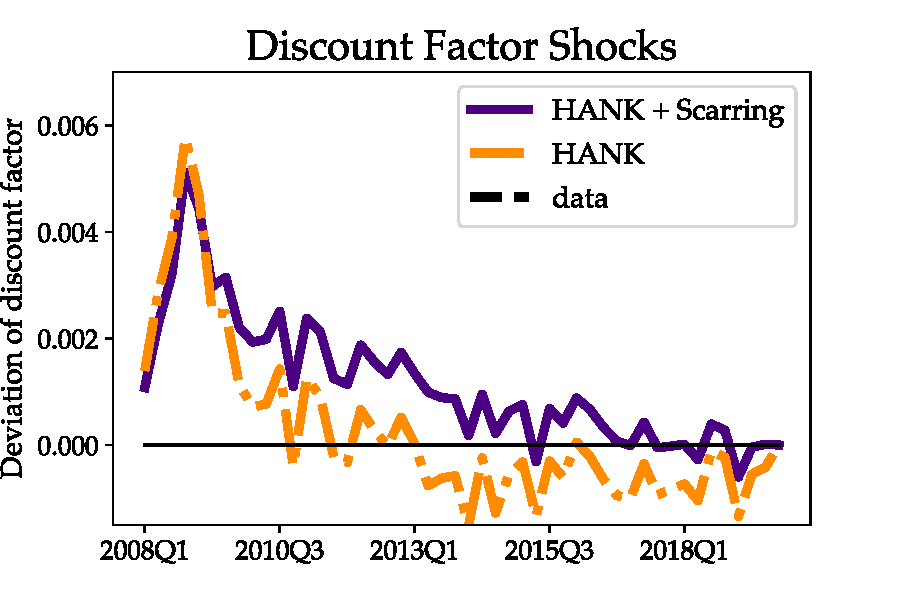
\includegraphics[scale=.5]{text/chapter1/Figures/GR_sim/DiscFacShks}
\end{minipage}\hspace*{\fill}
\begin{minipage}{0.5\textwidth}
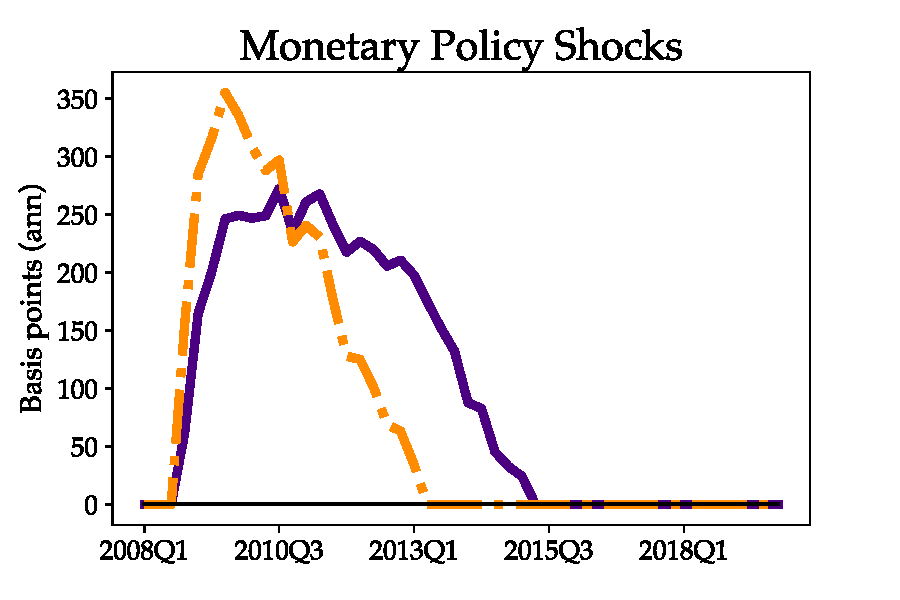
\includegraphics[scale=.5]{text/chapter1/Figures/GR_sim/EVShocks}
\end{minipage}
\medskip
\begin{minipage}{0.5\textwidth}
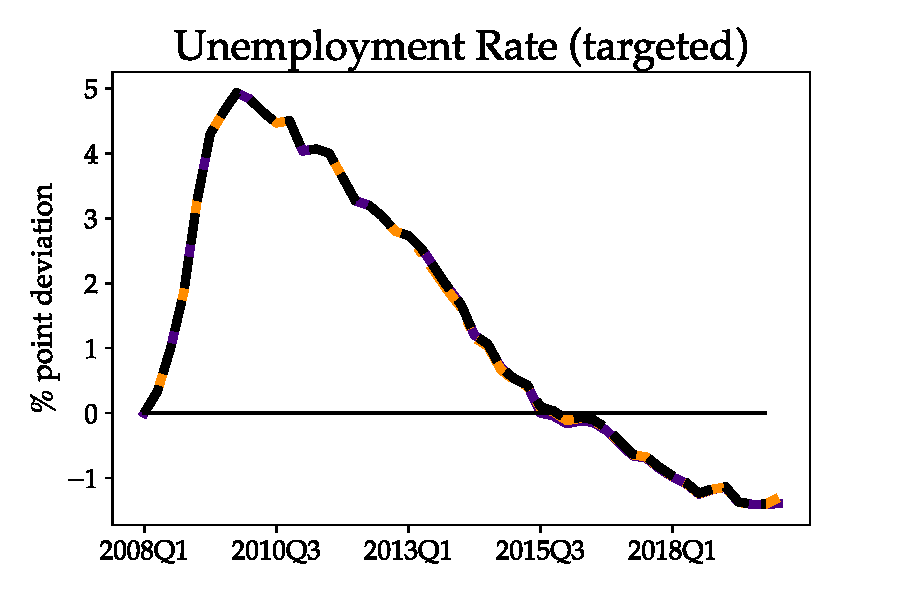
\includegraphics[scale=.5]{text/chapter1/Figures/GR_sim/Urate_}
\end{minipage}\hspace*{\fill}
\begin{minipage}{0.5\textwidth}
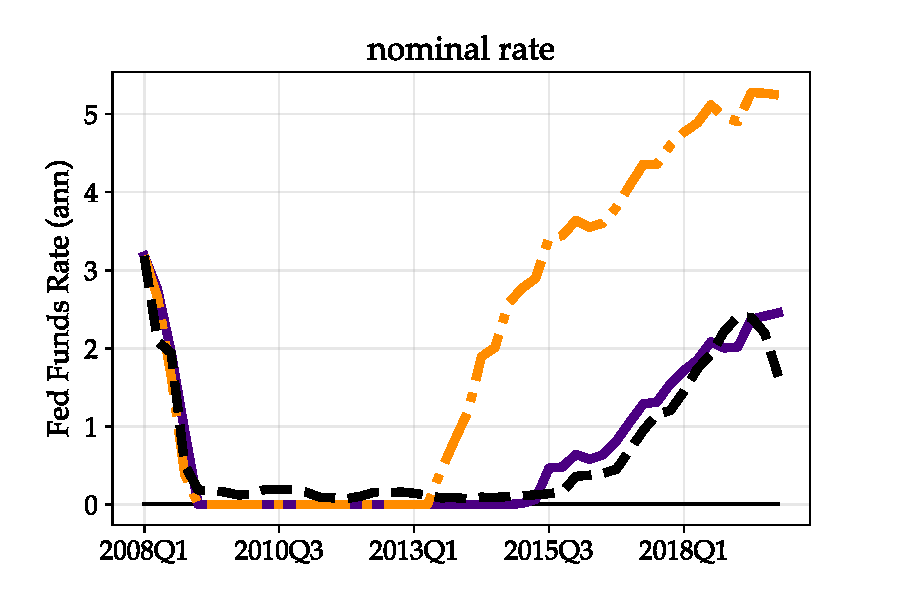
\includegraphics[scale=.5]{text/chapter1/Figures/GR_sim/FedFunds}
\end{minipage}
\caption{Estimated shocks to discount factor and nominal rate} 
\label{Estimatedshks}
\end{center}
\end{figure}


For the estimation, I follow \cite{kekre2023} and jointly estimate a sequence of discount factor shocks to match the path of unemployment from 2008 to 2018 monetary policy shocks to account for the zero lower bound. I use discount factor shocks for parsimony as the goal of this exercise is not to answer what caused The Great Recession but to answer why did The Great Recession lead to such a slow recovery\footnote{The same simulation exercise can be reproduced with shocks to the household borrowing limit or to the job separation rate and would not affect the results below as unemployment scarring is present in the responses to all aggregate shocks in the model.}. For these discount factor shocks, I set the fiscal adjustment parameter to $\phi_{b} = 0.015$, the lower bound of the estimates documented by  \cite{AuclertMicroJumpsMacroHumps}, and assume that the government cannot adjust taxes for 40 quarters to obtain a more accurate assessment of the effects of the Great Recession on debt. When estimating these discount factor shocks, I assume all discount factors follow an AR(1) with quarterly persistence 0.95. As noted in \cite{kekre2023}, the chosen AR(1) persistence does not alter the results as a different persistence will alter the estimated sequences of shocks but not the path of unemployment as that is what is targeted. The monetary policy shocks are assumed to have no persistence. I repeat this procedure over a grid of different wage rigidities $\phi_{w}$ and choose the wage rigidity parameter that minimizes the squared distance between the response of price index and its counterpart in the data. To capture the effects of unemployment scarring, I repeat this procedure for the version of the model where unemployment scarring is turned off in the same manner as in section 6. 


\begin{figure}[H] % "[t!]" placement specifier just for this example
\centering
\begin{minipage}{0.51\textwidth}
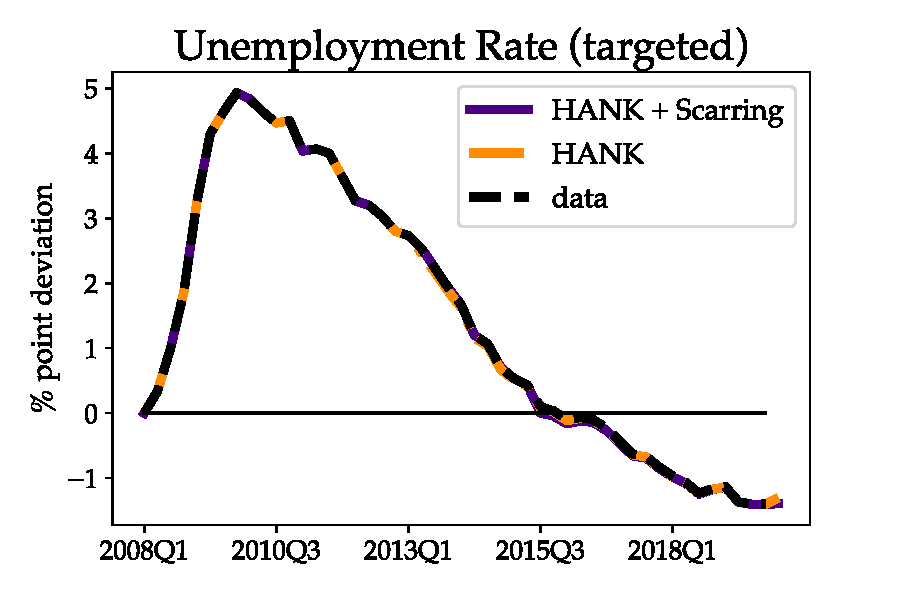
\includegraphics[scale=.55]{text/chapter1/Figures/GR_sim/Urate}
 \label{fig:a}
\end{minipage}\hspace*{\fill}
\begin{minipage}{0.51\textwidth}
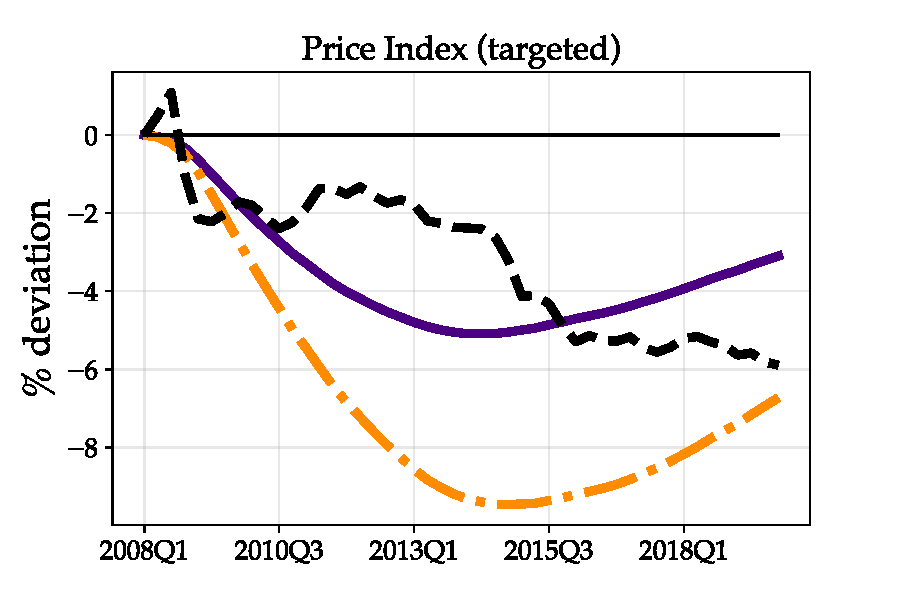
\includegraphics[scale=.55]{text/chapter1/Figures/GR_sim/PCE_defl}
 \label{fig:b}
\end{minipage}

\medskip
\begin{minipage}{0.51\textwidth}
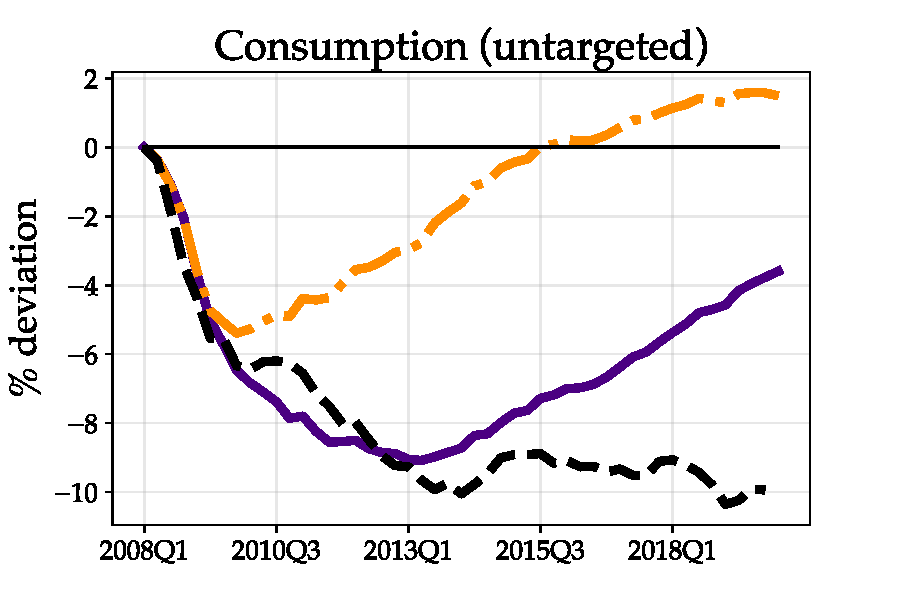
\includegraphics[scale=.55]{text/chapter1/Figures/GR_sim/PCE_IPR}
\label{fig:c}
\end{minipage}\hspace*{\fill}
\begin{minipage}{0.51\textwidth}
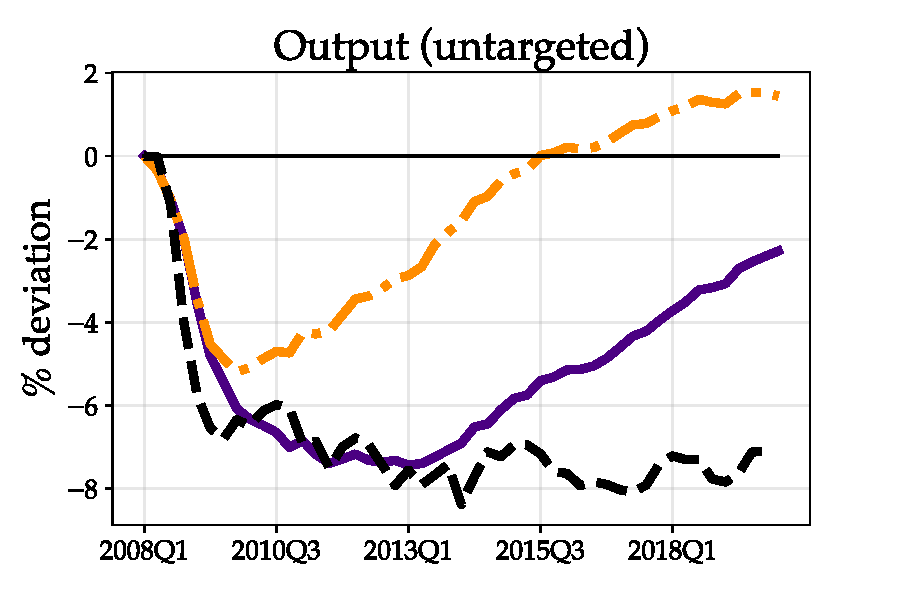
\includegraphics[scale=.55]{text/chapter1/Figures/GR_sim/GDP}
 \label{fig:d}
\end{minipage}

\medskip
\begin{minipage}{0.51\textwidth}
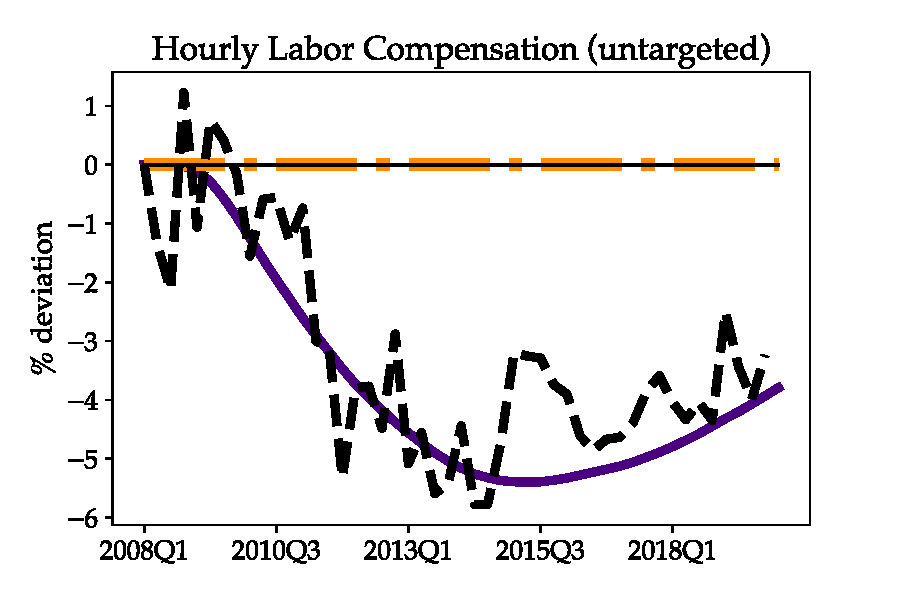
\includegraphics[scale=.55]{text/chapter1/Figures/GR_sim/Real_hourly_comp}
 \label{fig:e}
\end{minipage}\hspace*{\fill}
\begin{minipage}{0.51\textwidth}
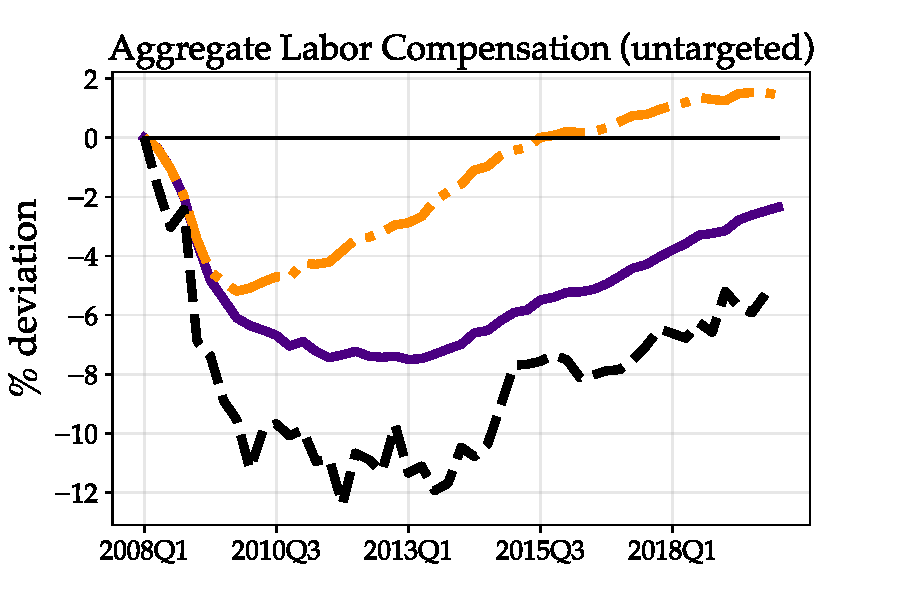
\includegraphics[scale=.55]{text/chapter1/Figures/GR_sim/labor_compensation}
 \label{fig:f}
\end{minipage}
\caption{Great Recession: Model vs Data (detrended)}
\floatfoot{Note: This figure compares the paths of various aggregates in the model with and without unemployment scarring to the data. The series display deviation from steady state for the model and from 2008Q1 for the data. In the data, real PCE, PCE deflator, real GDP, real hourly labor compensation, aggregate labor compensation are detrended from 1990Q1 to 2019Q4 and then rescaled such that the data represent deviation from 2008Q1.}
\label{NonTarget}
\end{figure}



\begin{figure}[H] % "[t!]" placement specifier just for this example
\centering
\begin{minipage}{0.51\textwidth}
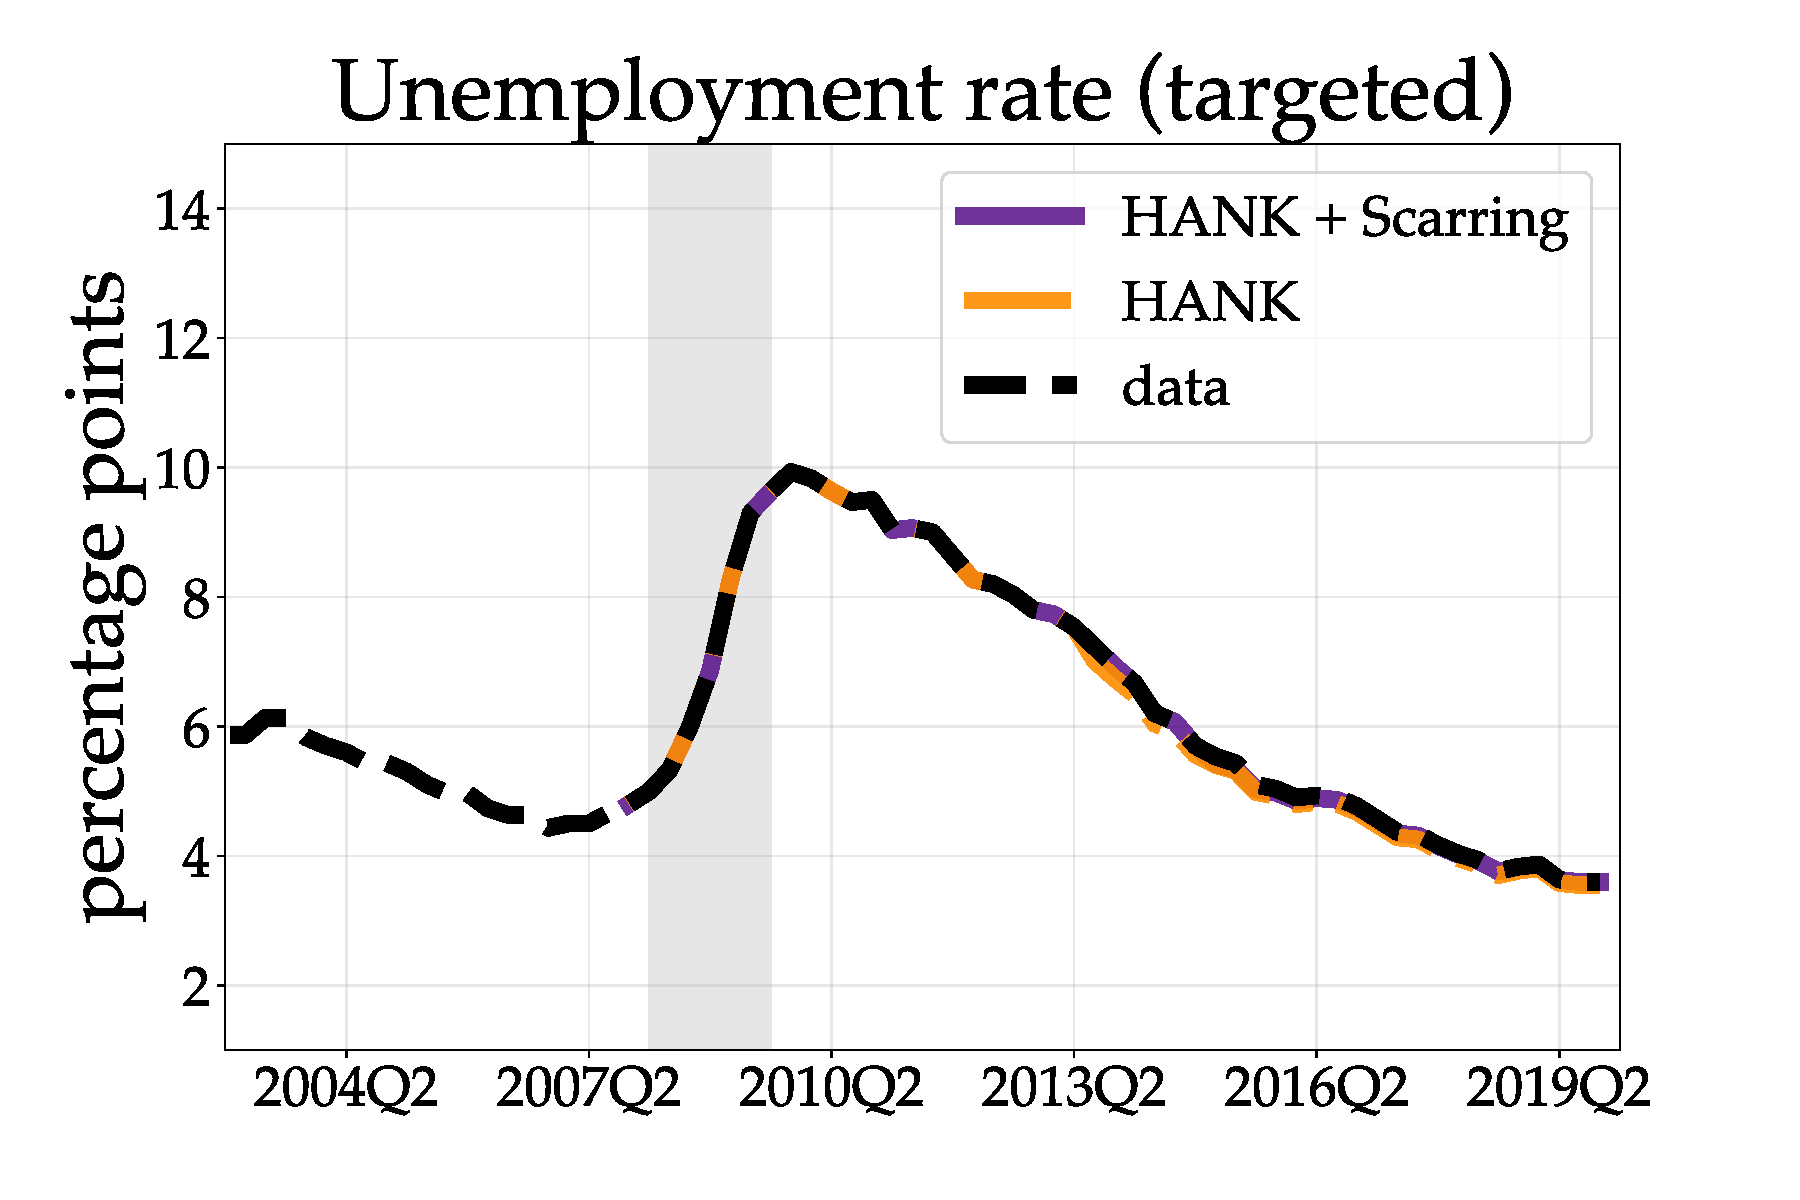
\includegraphics[scale=.29]{text/chapter1/Figures/GR_sim/Cleaner/Urate_vs_data_large_new}
 \label{fig:a}
\end{minipage}\hspace*{\fill}
\begin{minipage}{0.51\textwidth}
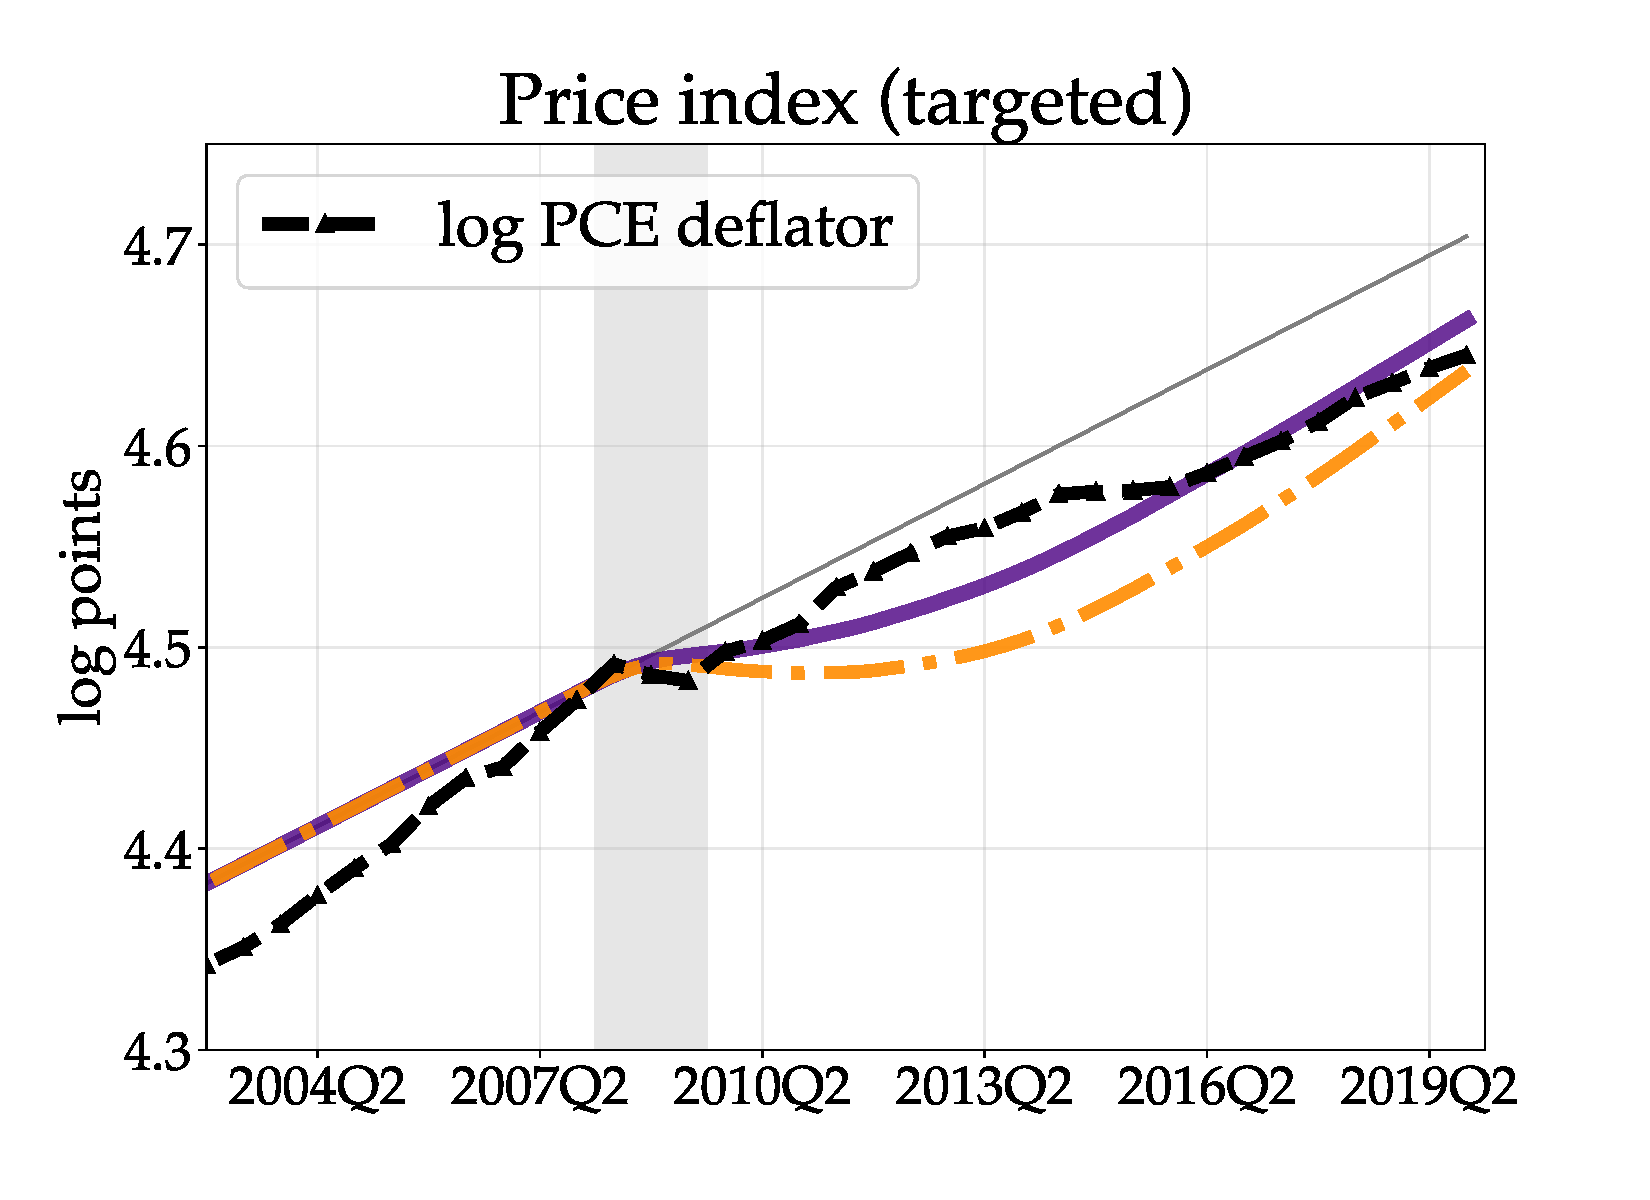
\includegraphics[scale=.29]{text/chapter1/Figures/GR_sim/Cleaner/price_vs_data_large_new}
 \label{fig:b}
\end{minipage}
\medskip
\begin{minipage}{0.51\textwidth}
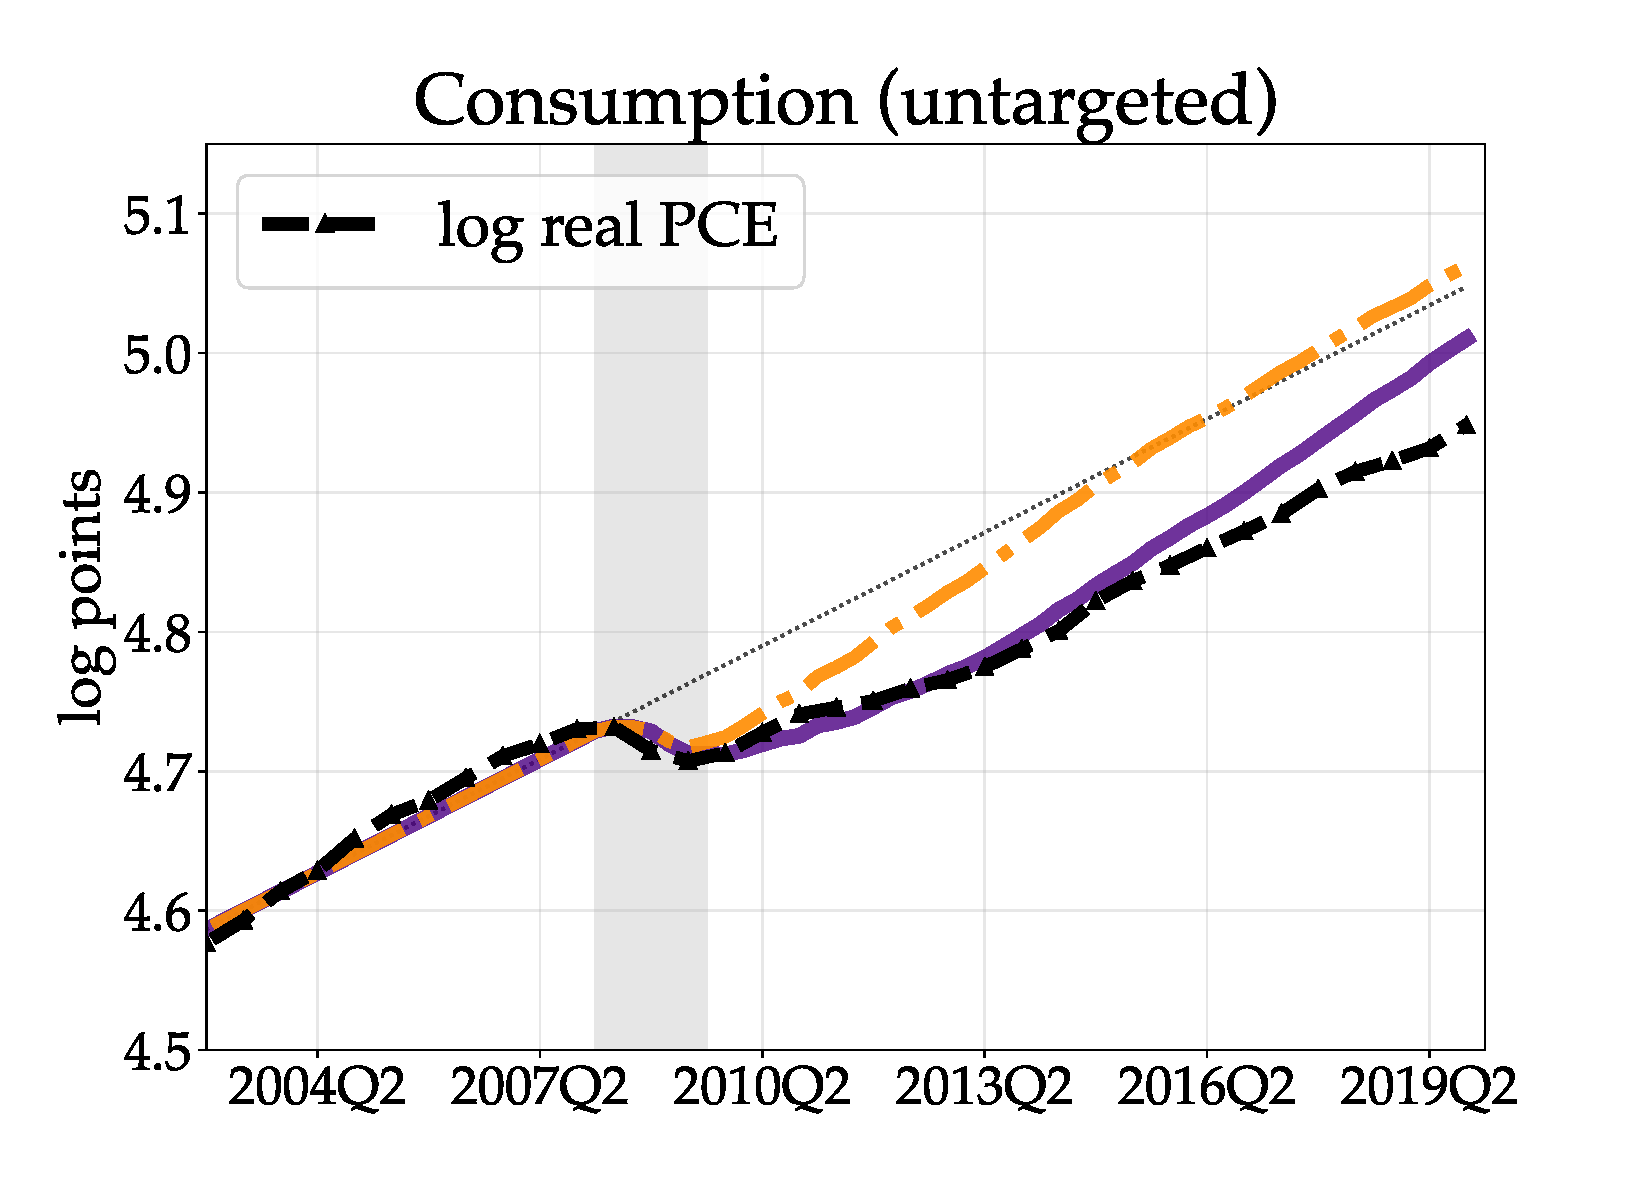
\includegraphics[scale=.29]{text/chapter1/Figures/GR_sim/Cleaner/Consumption_vs_data_large_new}
\label{fig:c}
\end{minipage}\hspace*{\fill}
\begin{minipage}{0.51\textwidth}
\includegraphics[scale=.29]{text/chapter1/Figures/GR_sim/Cleaner/Output_vs_data_large_new}
 \label{fig:d}
\end{minipage}
\medskip
\begin{minipage}{0.51\textwidth}
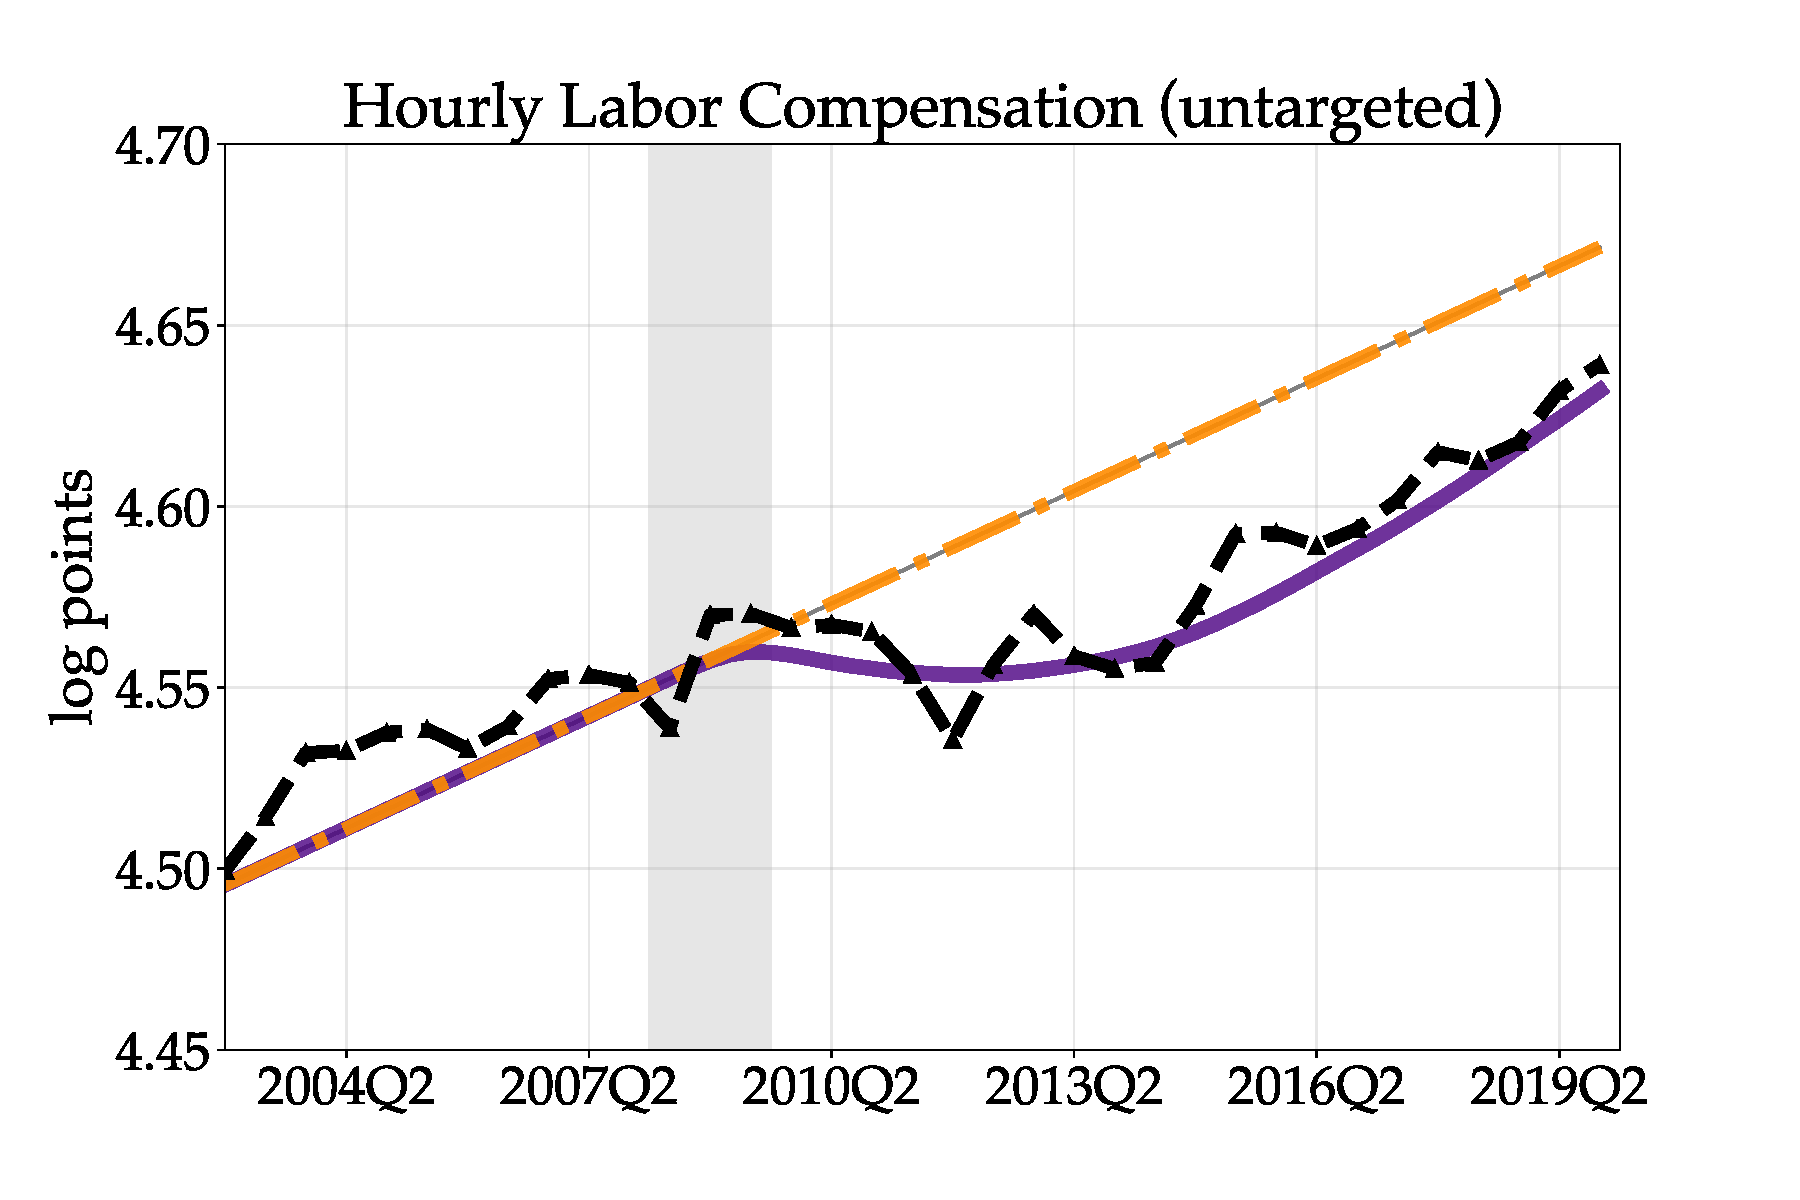
\includegraphics[scale=.29]{text/chapter1/Figures/GR_sim/Cleaner/hourly_comp_vs_data_large_new}
 \label{fig:e}
\end{minipage}\hspace*{\fill}
\begin{minipage}{0.51\textwidth}
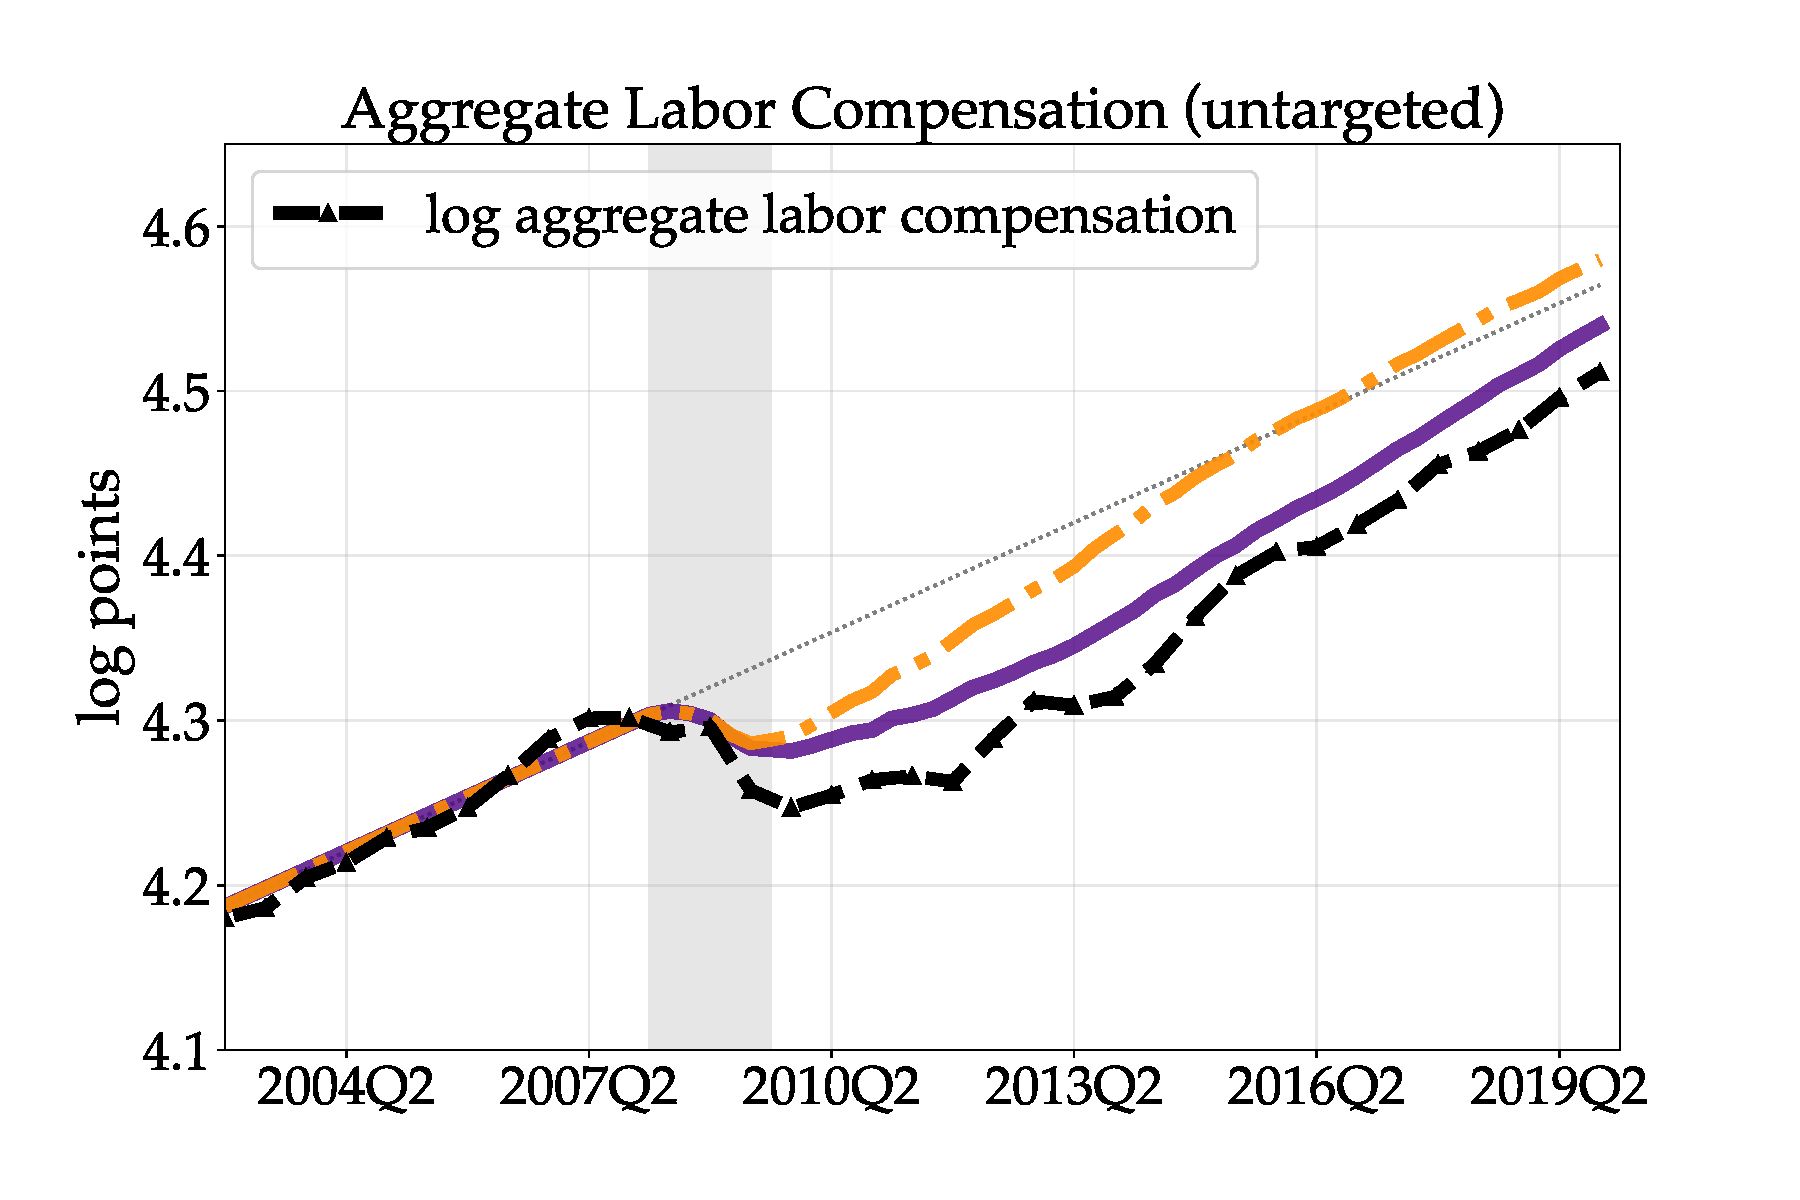
\includegraphics[scale=.29]{text/chapter1/Figures/GR_sim/Cleaner/labor_comp_vs_data_large_new}
 \label{fig:f}
\end{minipage}
\caption{Great Recession: Model vs Data (with trend)}
\floatfoot{Note: This figure plots the responses from figure \ref{NonTarget} with the trend.}
\label{NonTarget_with_trend}
\end{figure}


Figure \ref{Estimatedshks} plots the estimated shocks, the unemployment rate, and the nominal rate against the data under the baseline model and the model without scarring. Figure \ref{NonTarget} plots the key aggregate variables against their detrended observed counterpart in the data and \ref{NonTarget_with_trend} plots the model responses against the data without detrending. Only the unemployment rate and price index are targeted. 

Overall, unemployment scarring explains a substantial share of slow recovery following the Great Recession. In particular, scarring allows the model to match the path of the PCE and GDP until the beginning of 2015. Furthermore, the model under predicts the response of aggregate labor compensation likely due to the absence of labor force participation in the model. The path of hour labor compensation is matched especially well and provides macroeconomic validation that for unemployment scarring. Without unemployment scarring, the response of PCE, GDP, and aggregate labor compensation exhibit a 'V' shaped recovery as it mirrors the response of the unemployment rate. Unemployment scarring generates a persistent decline in labor productivity without a prolonged increase in the unemployment rate. This allows model to produce an income response that is significantly more persistent than the response of unemployment. 





\subsection{Debt to GDP during the Great Recession}


Having shown that the model can replicate the sluggish recovery from The Great Recession, in this section I evaluate the extent to which human capital losses increased debt to GDP during and after the Great Recession. Figure \ref{DebtGDP_sim} plots the simulated path of debt to GDP and tax revenues under the baseline model and the model without scarring. The model suggests that, by 2019, unemployment scarring increased debt to GDP by 5.5 $\%$ points. Human capital losses cause persistent losses in GDP as well as tax revenues which in turn increases debt.

\begin{figure}[!ht]
    \centering
   \begin{minipage}{0.48\textwidth}
        \centering
        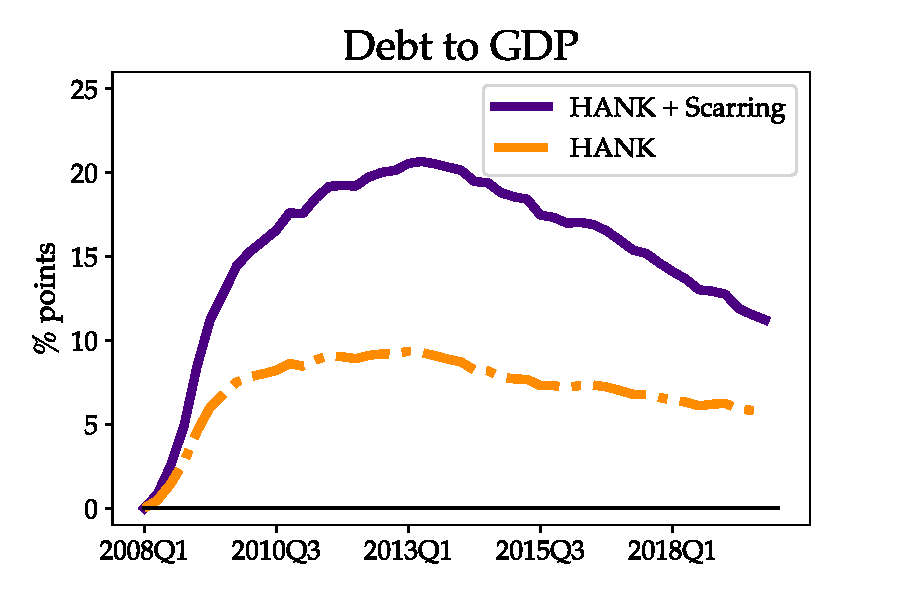
\includegraphics[scale=.57]{text/chapter1/Figures/GR_sim/debt2GDP_GR} % first figure itself
    \end{minipage}\hfill
    \begin{minipage}{0.48\textwidth}
        \centering
        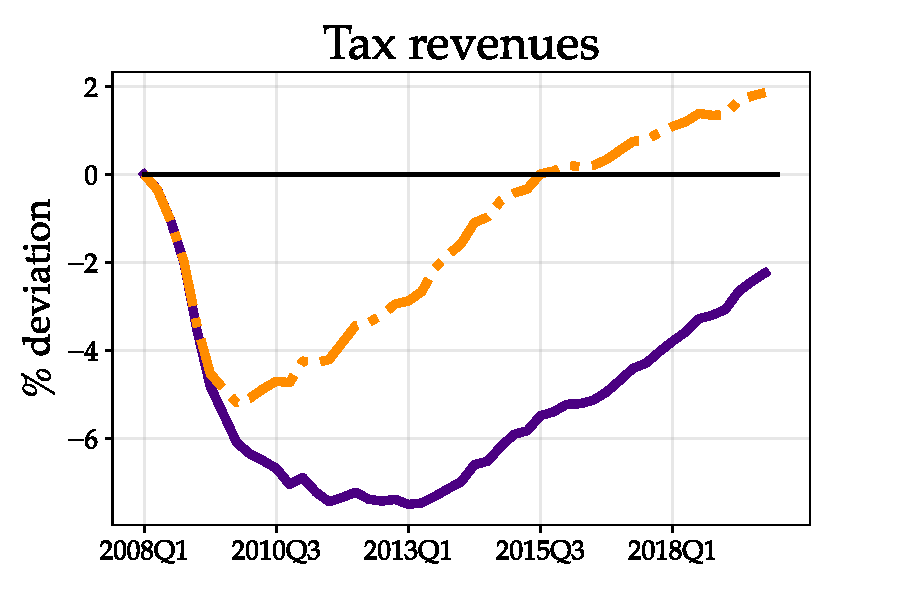
\includegraphics[scale=.57]{text/chapter1/Figures/GR_sim/tax_rev} % second figure itself
    \end{minipage}
    \caption{The response of debt to GDP and tax revenues}
    \label{DebtGDP_sim}
\end{figure}




\subsection{Income Inequality during the Great Recession}

Unemployment scarring increases the dispersion in human capital during a recession. As households become unemployment and later find reemployment at a lower wage, the variance of the distribution of wages increases persistently as the re-accumulation of human capital is slow.  Figure \ref{Gini_GR} shows that unemployment scarring allows the model to generate a near-permanent response in the Gini index of income that is consistent with the data. 


\begin{figure}[!ht!]
\begin{center}
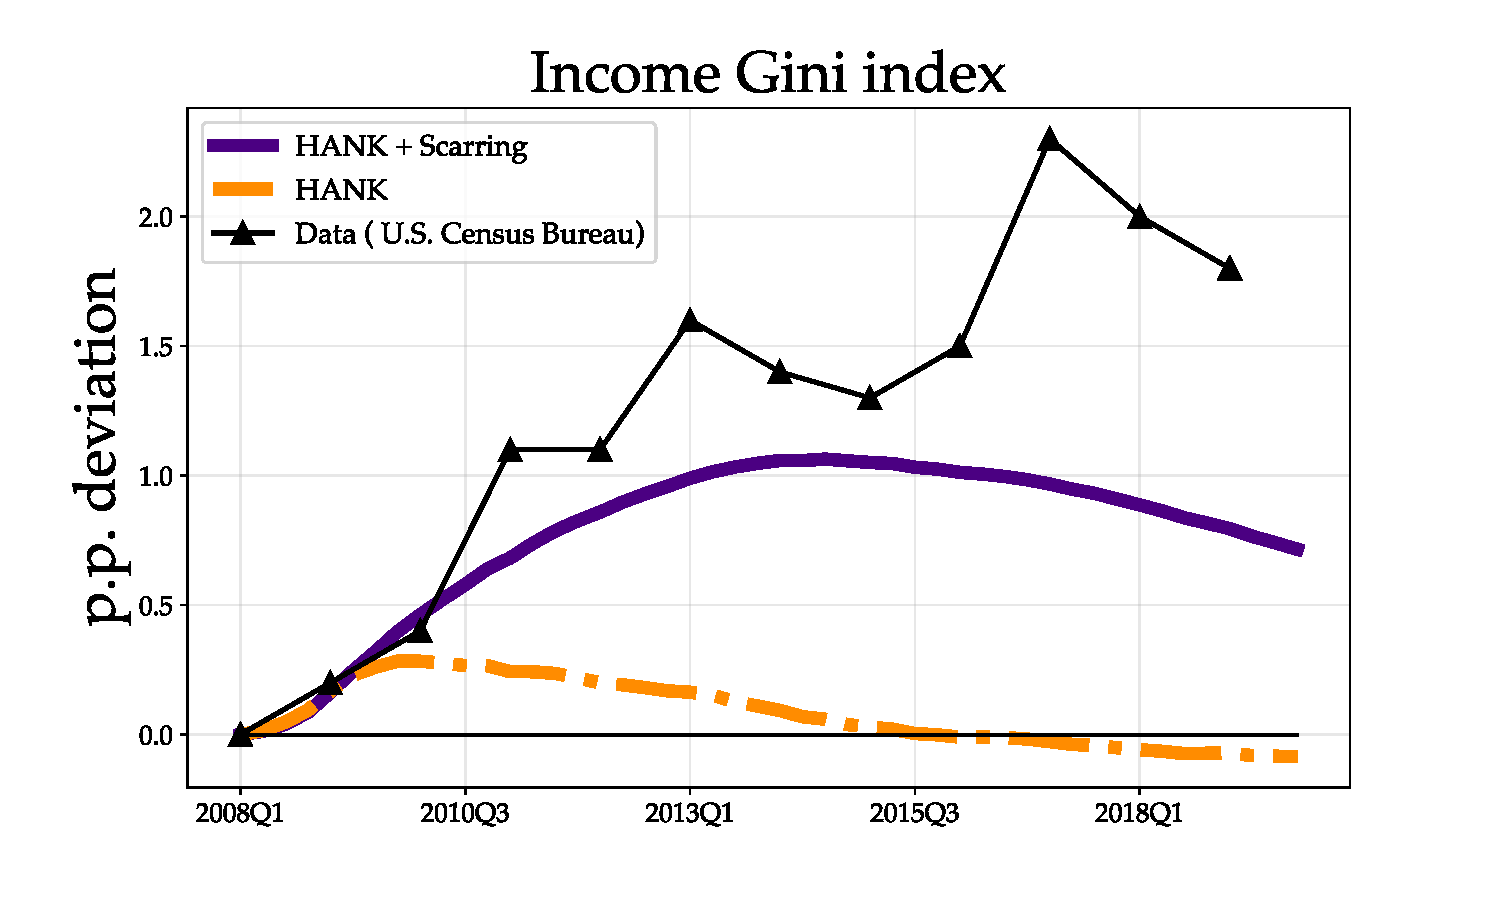
\includegraphics[scale=0.5]{text/chapter1/Figures/GR_sim/income_gini}
\end{center}
\caption{Gini Coefficient: Model vs Data}
 \label{Gini_GR}
\end{figure}






\section{The COVID Recession and Temporary Layoffs}


\subsection{The COVID Recession and the Absence of Scarring}

The behavior of unemployment during the COVID recession was unprecedented due to various reasons. One of these reasons is that 97.7$\%$ of the increase in the unemployment rate was attributed to temporary layoffs \citep{Gertler2022}. In this section, I show that, during the COVID recession, unemployment scarring did not translate to macro scarring because of the unprecedented fraction of temporary layoffs . Further, this section also shows that the model can explain both recessions with sluggish recoveries as well as recessions with quick recoveries. I repeat the estimation procedure of the previous section and recalibrate $\zeta^{X}$ for each unemployment state X to maximize the proportion of temporary layoffs that is attributed to a change in the unemployment rate. Further I assume that temporary layoffs cannot transition to a permanent layoff by setting $P_{TLPL} = 0$.\footnote{\cite{Gertler2022} note that 98$\%$ of these temporary layoffs do not transition to a permanent layoff.} At best, the model can attribute 78.5$\%$ of an increase in the unemployment rate to temporary layoffs.  Figure \ref{COVID_recession} plots the responses of unemployment rate, Gini index for income, consumption, output under the model with scarring calibrated to maximize the proportion of temporary layoffs (purple), and the version of the model without scarring (orange). With a large mass of temporary layoffs, the effects of unemployment scarring are effectively eliminated as temporary layoffs are reemployed at their pre-job layoff wage. The effective absence of unemployment scarring reduces the persistence of the responses of consumption and output in the baseline model leading leading the model to be consistent with the empirical paths of consumption and GDP. Further, the response of the Gini index is transitory, similar to the data. 

 

\begin{figure}[t!] % "[t!]" placement specifier just for this example
\centering
\begin{minipage}{0.51\textwidth}
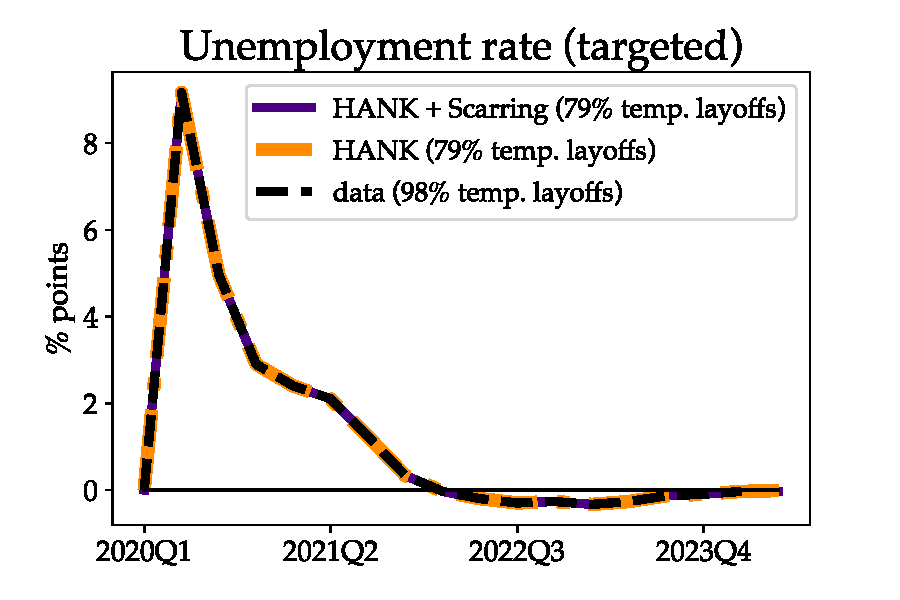
\includegraphics[scale=.57]{text/chapter1/Figures/pandemic_sim/Urate_pandemic}
 \label{fig:a}
\end{minipage}\hspace*{\fill}
\begin{minipage}{0.51\textwidth}
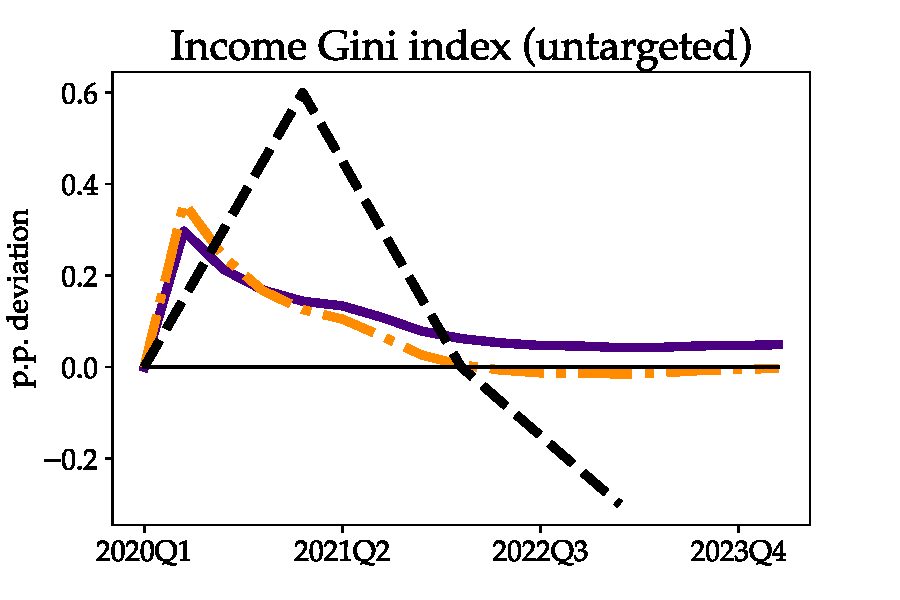
\includegraphics[scale=.57]{text/chapter1/Figures/pandemic_sim/income_gini_pandemic}
 \label{fig:b}
\end{minipage}




\medskip
\begin{minipage}{0.51\textwidth}
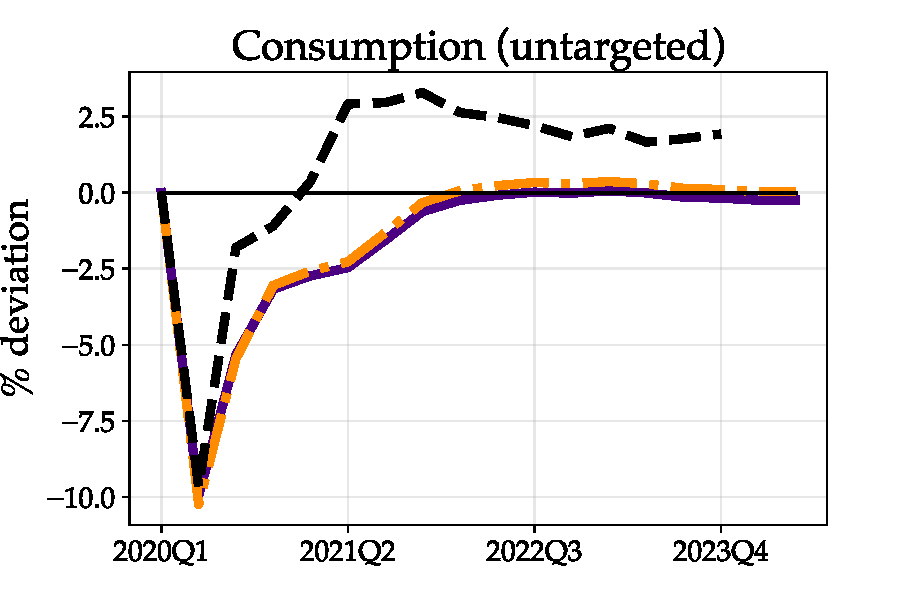
\includegraphics[scale=.57]{text/chapter1/Figures/pandemic_sim/C_pandemic}
\label{fig:c}
\end{minipage}\hspace*{\fill}
\begin{minipage}{0.51\textwidth}
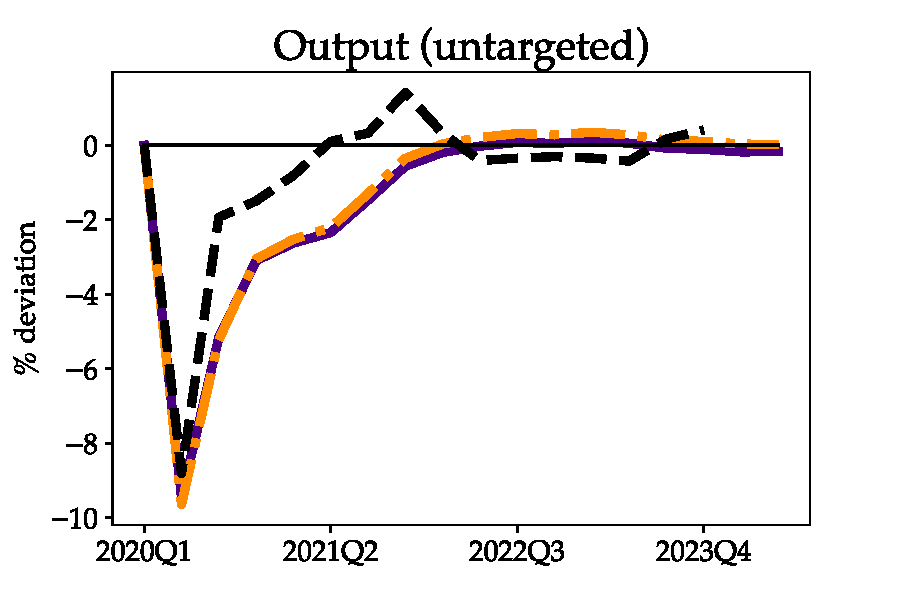
\includegraphics[scale=.57]{text/chapter1/Figures/pandemic_sim/GDP_pandemic}
 \label{fig:d}
\end{minipage}
\caption{Model vs data: The COVID Recession}
\floatfoot{Note: In this exercise, the effects unemployment scarring are eliminate when the model is recalibrated to match the large proportion of temporary layoffs that explain the rise in unemployment. In particular, for this calibration, 78.5 $\%$ of the increase in the unemployment rate is attributed to temporary layoffs. Empirically, $97.7 \%$ of the increase in the unemployment rate is due to temporary layoffs. The model is unable to account for such a large proportion of temporary layoffs because the fall in labor market tightness during the simulation lowers the job finding probability of those who were already in a  permanently layoff prior to the recession. Thus, the duration of those permanent layoffs rises.}

\label{COVID_recession}

\end{figure}



\subsection{Temporary Layoffs and Swift Recoveries}


In this section, I demonstrate that temporary layoffs,  following the COVID recession,  were instrumental in both accelerating the swift recovery of GDP and in preventing a permanent rise in income inequality. To show this, I repeat the estimation procedure of matching the unemployment rate during the COVID Recession but recalibrate the model to maximize the fraction of permanent layoffs that can be attributed to an increase in the unemployment rate. Because the job probabilities of workers who are in temporary layoff falls endogenously with the unemployment rate, the duration of a temporary layoff rises therefore preventing the model from producing an increase in an unemployment rate that is entirely explained by permanent layoff.\footnote{In other words, even if the increase in the EU probability in this simulation is completely captured by permanent layoffs, the UE probability of workers who were in temporary layoff prior to the recession must also fall.}

Figure \ref{COVID_Counterfactual_GDP} and figure \ref{COVID_Counterfactual_gini} compares the path of output and income Gini, respectively, under the original calibration (from section 9.1) against the counterfactual scenario with a large fraction of permanent layoffs. In all lines in each figure, the path of unemployment remains identical and instead only differs in the composition of the unemployment rate between permanent and temporary layoffs. Figure \ref{COVID_Counterfactual_GDP} demonstrates that if the rise in unemployment has been primarily due to permanent layoffs, GDP would not have returned to its pre-recessionary trend. Although the long run difference between the counterfactual and the data may appear small ---due to the sharp initial contraction in GDP--- the percentage deviation of the counterfactual from the trend reaches 2 $\%$ by the second quarter of 2023. This magnitude is within range of long run output deviations observed after the 1990-1991 and 2000s recessions. Moreover, emphasizing the role of temporary layoffs does not diminish the significance of fiscal policy in shaping the recovery from the pandemic. Fiscal measures may have contributed to the large proportion of temporary layoffs during the COVID Recession. Overall, temporary layoffs were a key factor in enabling GDP to return to its pre-recessionary trend and likely complemented the effectiveness of fiscal stimulus during this period. Similarly, Figure \ref{COVID_Counterfactual_gini} illustrates that temporary layoffs prevented the permanent rise in the Gini index for income. Notably, the red line demonstrates that if the majority of the increase in the unemployment rate was due to permanent layoffs, then the Gini index for income would have permanently risen.  




\begin{figure}[!ht!]
\begin{center}
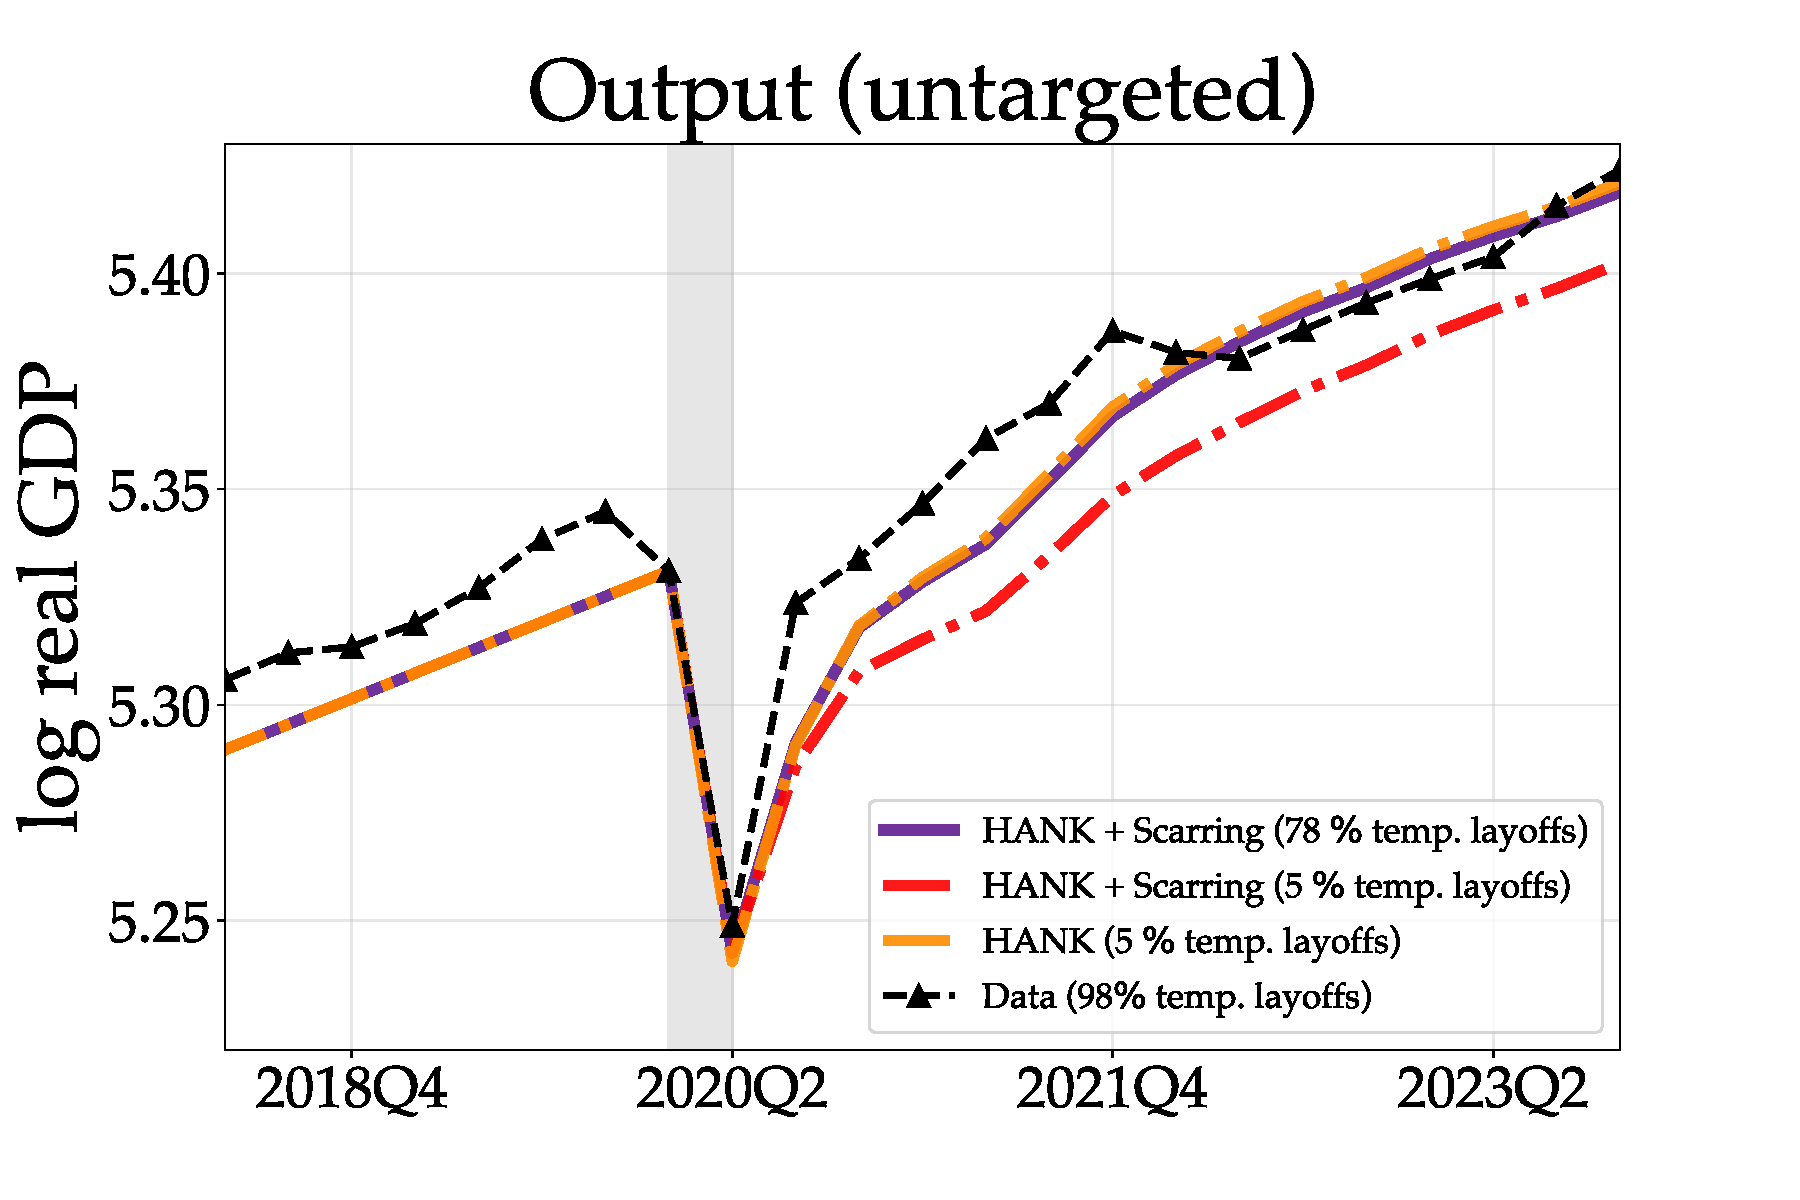
\includegraphics[scale=.53]{text/chapter1/Figures/pandemic_counterfactual/output_vs_data_jam_COVID_counterfactual}
\end{center}
\caption{Counterfactual for GDP: What if the rise in unemployment during the pandemic was due to permanent layoffs? }
\floatfoot{This figure plots the paths of output with trend from the HANK + Scarring model (purple) under the baseline COVID calibration (with 78$\%$ temporary layoffs) against a counterfactual (red) where the rise in unemployment during COVID is largely explained by permanent layoffs. Note that for both paths of output, the unemployment rate is identical. Only the composition of the unemployment rate differs. }
\label{COVID_Counterfactual_GDP}
\end{figure}



\begin{figure}[!ht!]
\begin{center}
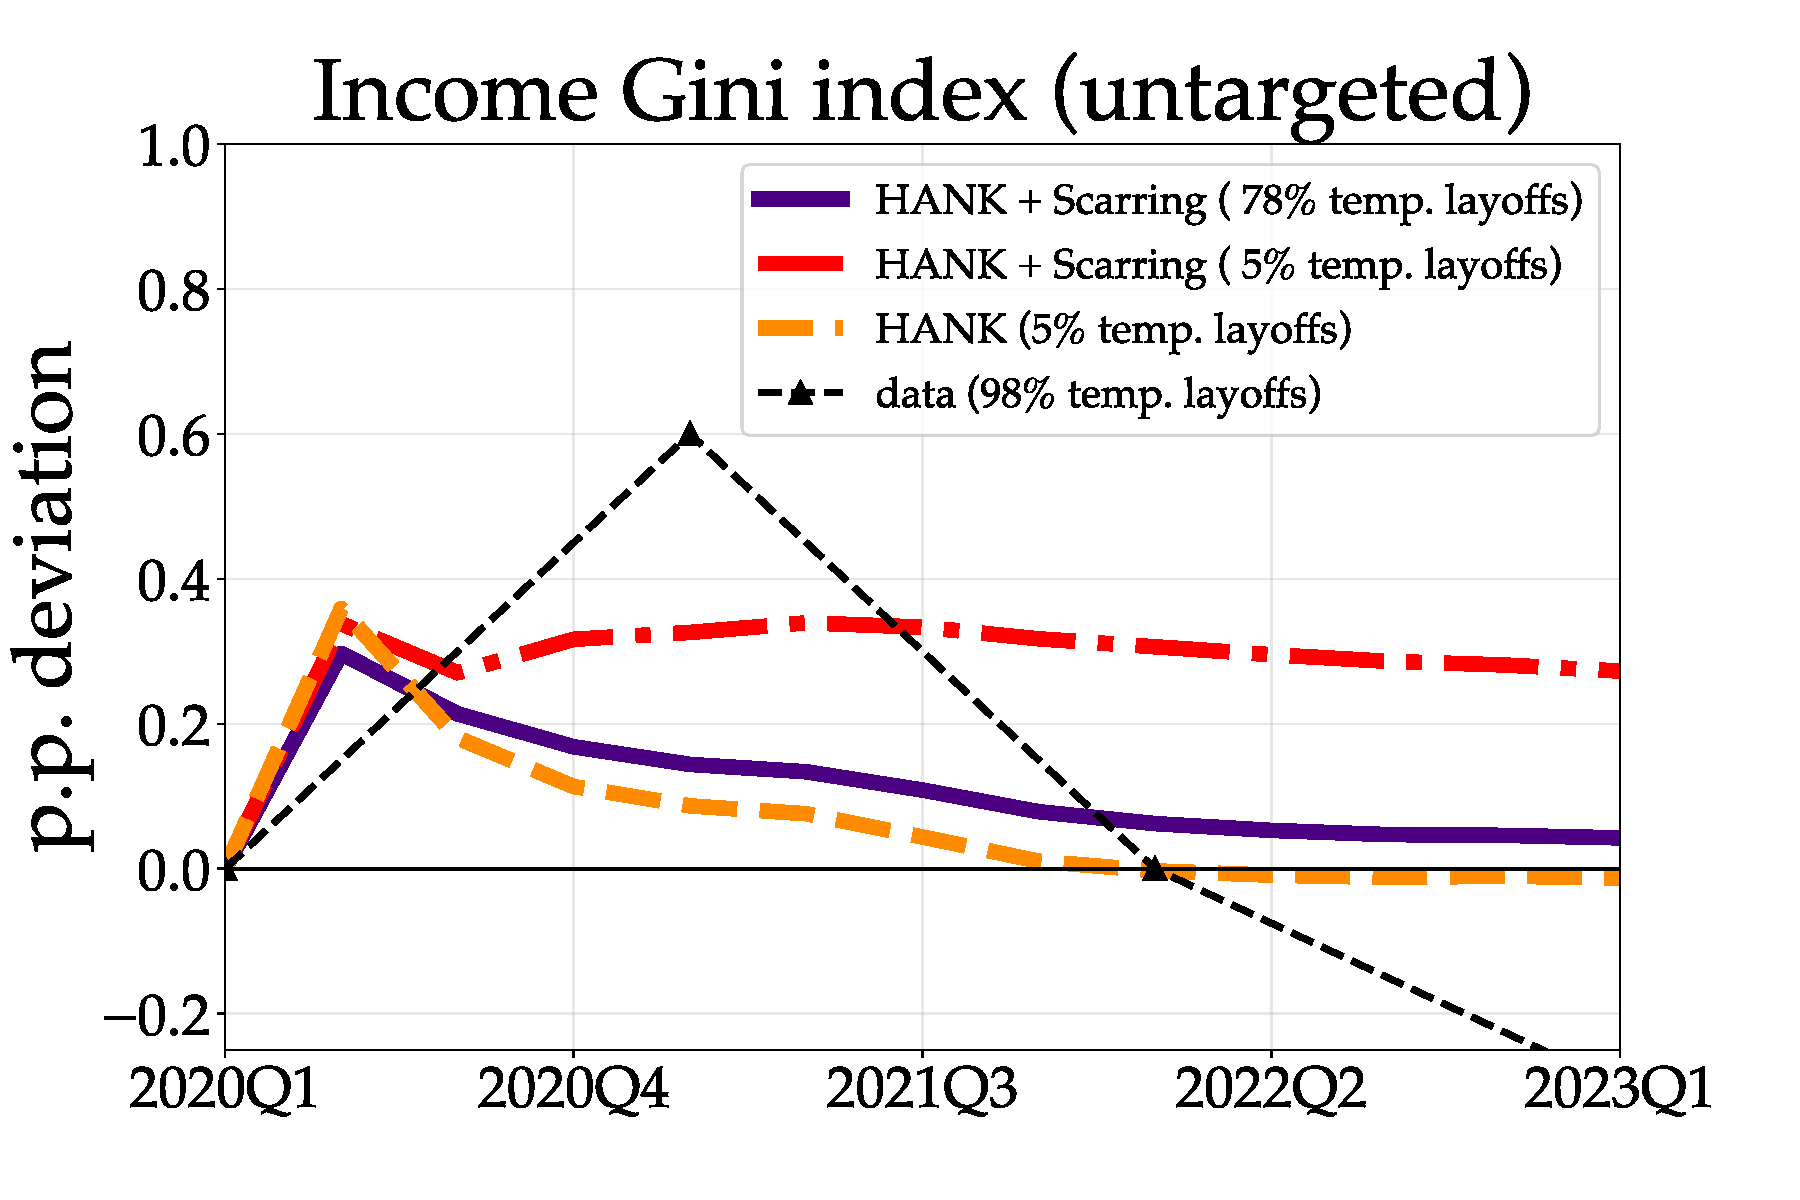
\includegraphics[scale=.53]{text/chapter1/Figures/pandemic_counterfactual/income_gini_pandemic_counterfactual_perm_only}
\end{center}
\caption{Counterfactual for Gini index: What if the rise in unemployment during the pandemic was due to permanent layoffs?}
\floatfoot{This figure plots the paths of the income Gini index from the HANK + Scarring model (purple) under the baseline COVID calibration (with 78$\%$ temporary layoffs) against a counterfactual (red) where the rise in unemployment during COVID is largely explained by permanent layoffs. Note that for both paths of the income Gini index, the unemployment rate is identical. Only the composition of the unemployment rate differs. }
\label{COVID_Counterfactual_gini}
\end{figure}




\section{What if the US had pursued fiscal consolidation during the Great Recession?}


\subsection{A Reductions in Government Transfers in 2010}

During The Great Recession, while the US pursued fiscal stimulus, European countries engaged in large fiscal consolidations. These austerity measures led to large contractions in GDP \citep{Jorda2016,FATAS2018,House2020}. Further, unemployment scarring has been shown to be very much present, and slightly worse, in Europe.\footnote{\cite{Bertheau2023} } In this section, I consider the path of the US economy had it engaged in similar austerity measures. I augment the simulation in the previous section by simulating a counterfactual where the US reduces government spending by $2\%$ of GDP at the beginning of 2010. I assume the shock has a quarterly persistence of 0.9 such that its path fades by 2016. As in the Great Recession simulation, the tax rate cannot adjust for 10 years and set $\phi_{b}=0.015$. To account for the zero lower bound, I set the the coefficients of the Taylor rule on output, $\phi_{Y}$, and inflation, $\phi_{\pi}$, to zero such that the central bank fixes the nominal rate in response to this shock. I augment the estimated demand and monetary policy shocks from the previous section with this fiscal consolidation shock and simulate the path of the economy. Figure \ref{FC_US} plots the deviation in government spending, GDP, debt to GDP, and debt in the baseline simulation (purple), the simulation with fiscal consolidation (red), and the path of these aggregates without human capital losses (green dashed). In figure \ref{FC_US}, fiscal consolidation causes a persistent decline in GDP while only generating a slight decline a debt and debt to GDP. In particular, the decrease in government spending of  $2\%$ of GDP only decreases debt to GDP by $1.23$ percentage points. In the absence of human capital losses from scarring, the green dashed line demonstrates that debt to GDP would have fallen by $4.75$ percentage points. Overall, fiscal consolidation during the Great Recession would have generated a large and persistent decline in GDP while being ineffective at reducing debt to GDP.


\begin{figure}[t!] % "[t!]" placement specifier just for this example
\centering
\begin{minipage}{0.51\textwidth}
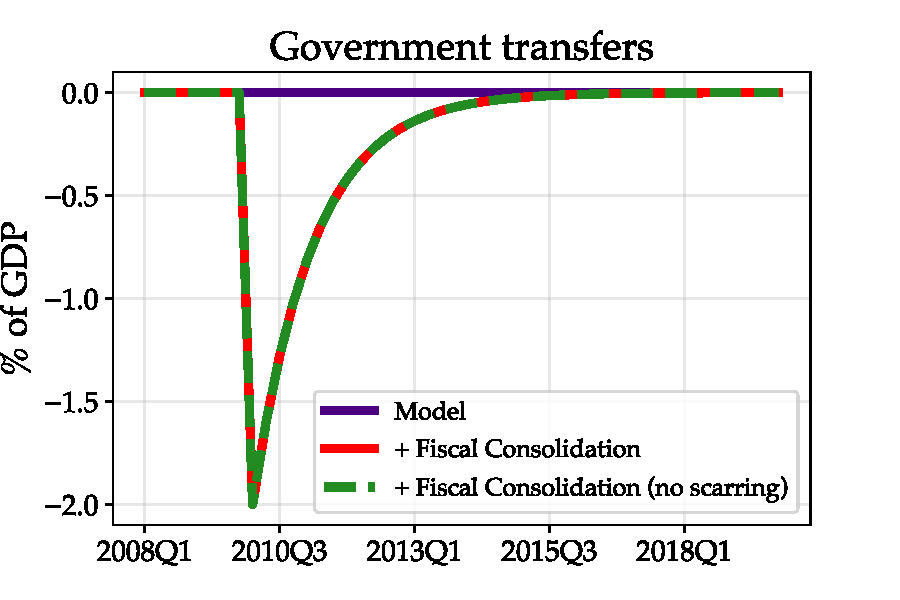
\includegraphics[scale=.57]{text/chapter1/Figures/Fiscal_Consolidation_CounterFactual/transfer_shocks_fiscal_consolidation}
 \label{fig:a}
\end{minipage}\hspace*{\fill}
\begin{minipage}{0.51\textwidth}
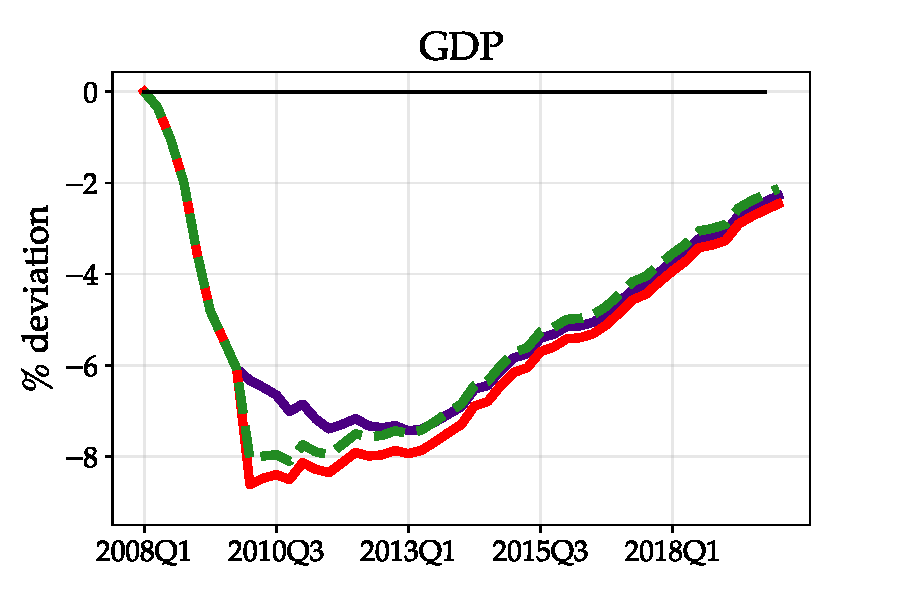
\includegraphics[scale=.57]{text/chapter1/Figures/Fiscal_Consolidation_CounterFactual/GDP_CounterFactual_Fiscal_Consolidation}
 \label{fig:b}
\end{minipage}

\medskip
\begin{minipage}{0.51\textwidth}
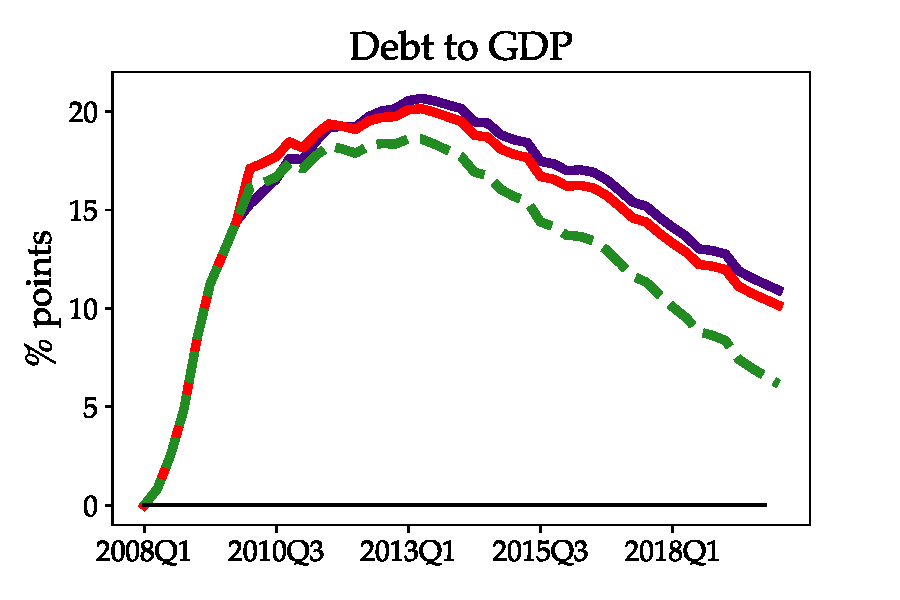
\includegraphics[scale=.57]{text/chapter1/Figures/Fiscal_Consolidation_CounterFactual/debt2GDP_CounterFactual_Fiscal_Consolidation}
\label{fig:c}
\end{minipage}\hspace*{\fill}
\begin{minipage}{0.51\textwidth}
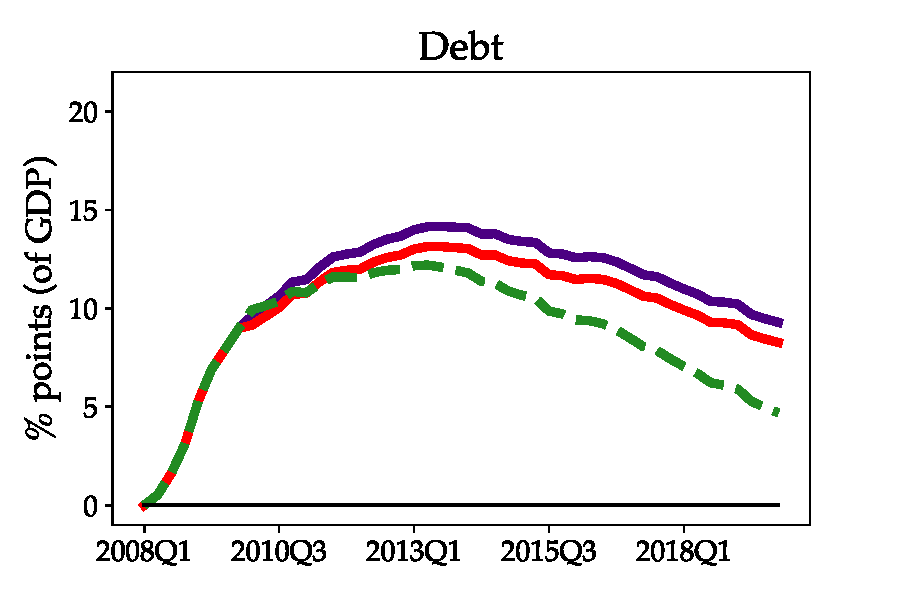
\includegraphics[scale=.57]{text/chapter1/Figures/Fiscal_Consolidation_CounterFactual/debt_CounterFactual_Fiscal_Consolidation}
 \label{fig:d}
\end{minipage}
\medskip
\begin{minipage}{0.51\textwidth}
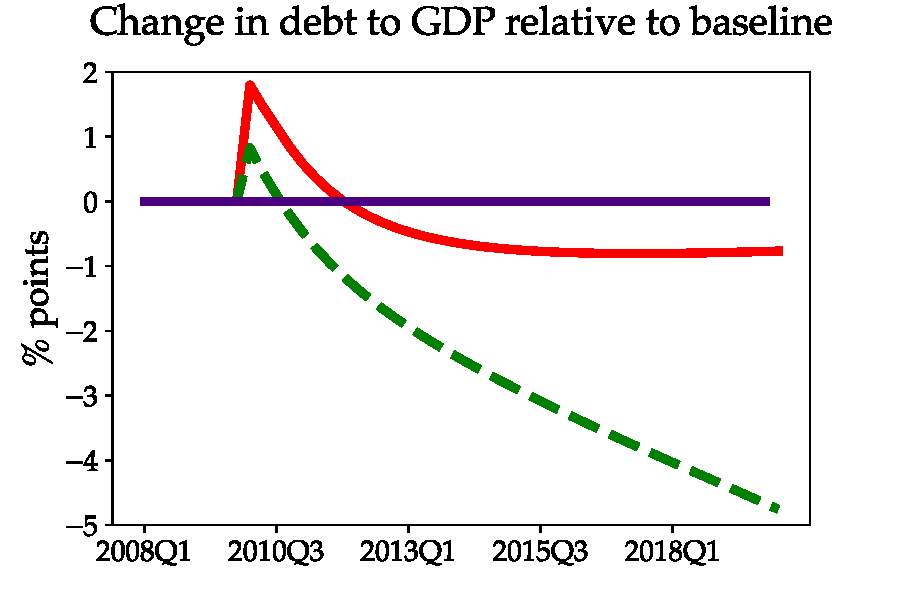
\includegraphics[scale=.57]{text/chapter1/Figures/Fiscal_Consolidation_CounterFactual/change_in_debt2GDP_CounterFactual_Fiscal_Consolidation}
\label{fig:c}
\end{minipage}\hspace*{\fill}
\begin{minipage}{0.51\textwidth}
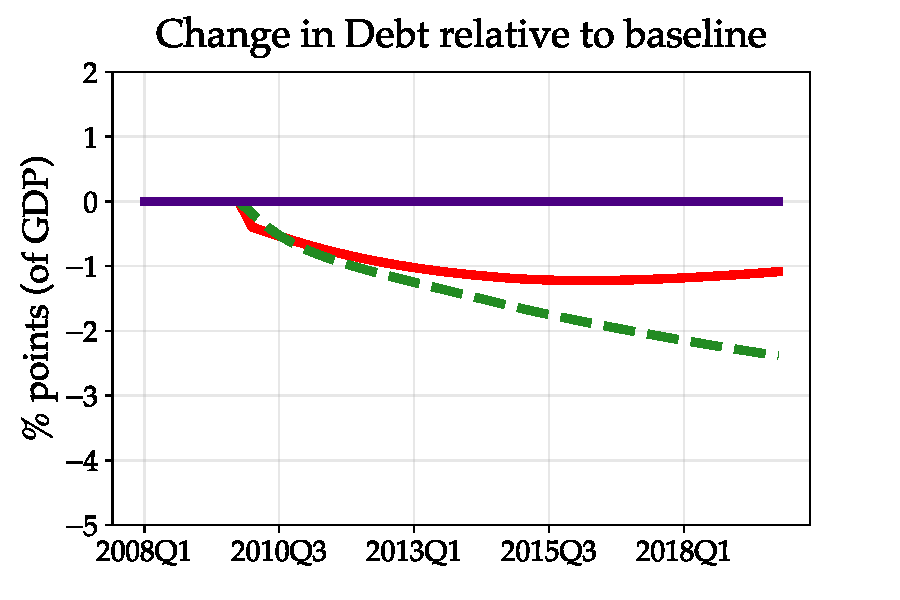
\includegraphics[scale=.57]{text/chapter1/Figures/Fiscal_Consolidation_CounterFactual/change_in_debt_CounterFactual_Fiscal_Consolidation}
 \label{fig:d}
\end{minipage}

\caption{Counterfactual: Fiscal Consolidation in the US}
\floatfoot{Note: This exercise plots the simulated paths of of macro aggregates during the Great Recession from figure \ref{NonTarget} with a fiscal consolidation shock that begins in 2010Q1 under the baseline model and the model without scarring.}

\label{FC_US}
\end{figure}


\hypertarget{Fiscal Consolidation and the Zero Lower Bound}{}
\subsection{Fiscal Consolidation and the Zero Lower Bound}

What are the effects of the zero lower bound on the counterfactual fiscal consolidation in section 7.3? To do so, I redo the experiment in section 7.3 but allow for an active Taylor rule. In particular, I set the Taylor rule coefficient on output, $\phi_{Y}$, to $1/12$ and the Taylor rule coefficient on inflation, $\phi_{\pi}$, to $1.5$.  Further, to illustrate the effect of an aggressive monetary authority, I also perform this experiment again with $\phi_{Y} = 0.2$ Figure \ref{FC_US_no_ZLB} plots the fiscal consolidation exercise with and without the zero lower bound under the baseline Taylor rule and the more aggressive Taylor rule. Without the zero lower bound, fiscal consolidation becomes significantly more effective at reducing debt to GDP. The dashed blue and orange lines demonstrates that the decline in debt to GDP is substantially larger without the zero lower bound. The increased effectiveness of fiscal consolidation in reducing debt to GDP in the absence of the zero lower bound stems from decreasing the cost of debt. Decreasing the interest rate alleviates the fiscal authority's cost of borrowing, and therefore decreases the upward pressure that lost tax revenues place on debt. 


\begin{figure}[t!] % "[t!]" placement specifier just for this example
\centering
\begin{minipage}{0.51\textwidth}
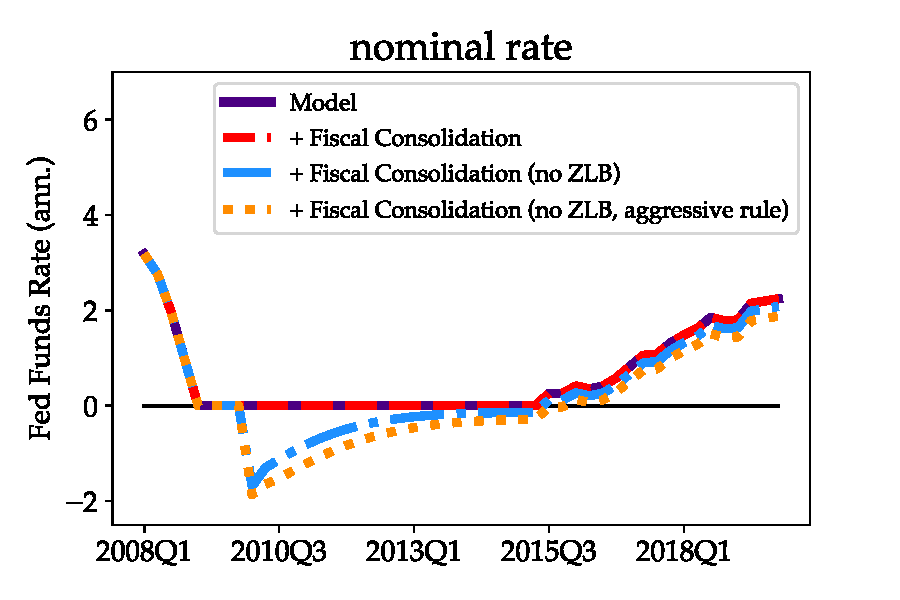
\includegraphics[scale=.57]{text/chapter1/Figures/Fiscal_Consolidation_CounterFactual/FedFunds_FC_no_ZLB_lower}
 \label{fig:a}
\end{minipage}\hspace*{\fill}
\begin{minipage}{0.51\textwidth}
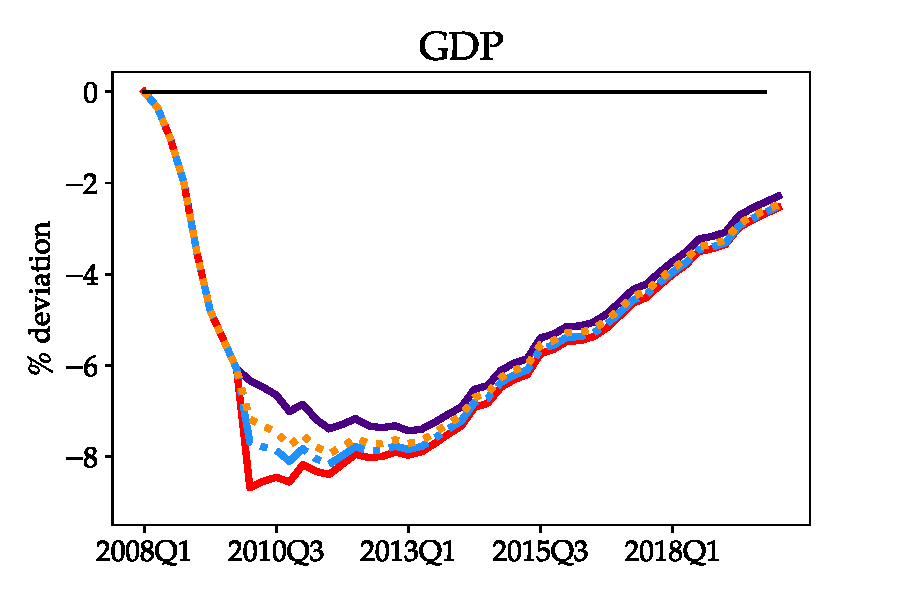
\includegraphics[scale=.57]{text/chapter1/Figures/Fiscal_Consolidation_CounterFactual/GDP_CounterFactual_Fiscal_Consolidation_no_ZLB_lower}
 \label{fig:b}
\end{minipage}

\medskip
\begin{minipage}{0.51\textwidth}
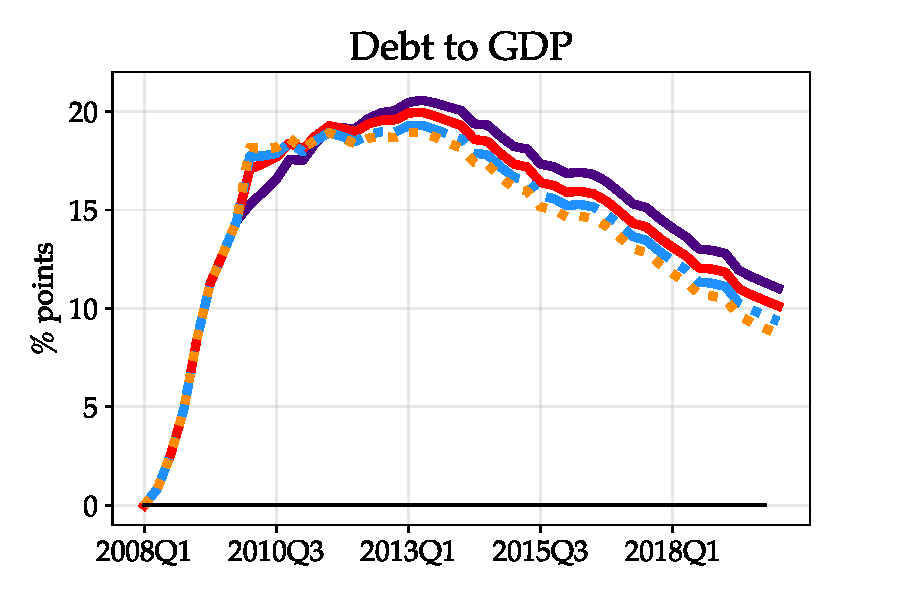
\includegraphics[scale=.57]{text/chapter1/Figures/Fiscal_Consolidation_CounterFactual/debt2GDP_CounterFactual_Fiscal_Consolidation_no_ZLB_lower}
\label{fig:c}
\end{minipage}\hspace*{\fill}
\begin{minipage}{0.51\textwidth}
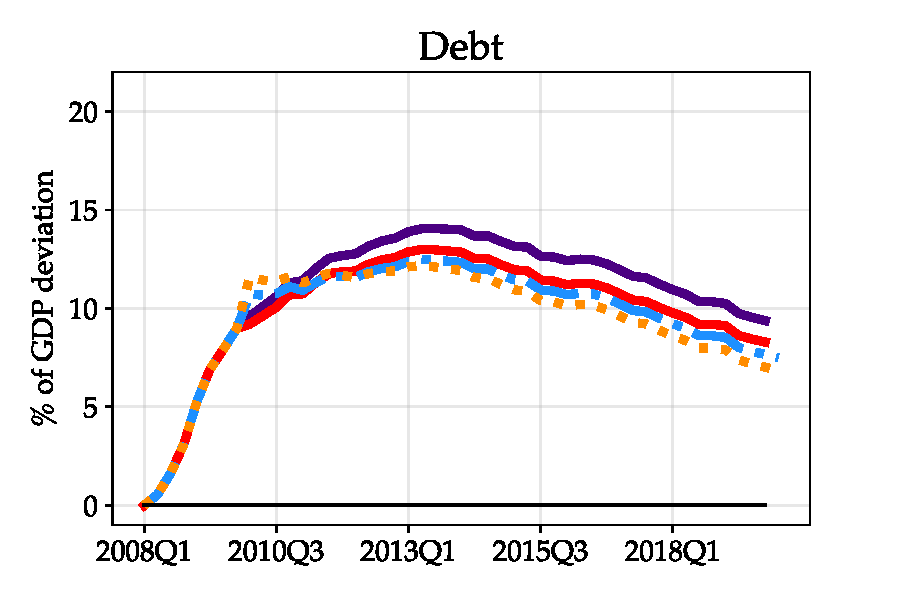
\includegraphics[scale=.57]{text/chapter1/Figures/Fiscal_Consolidation_CounterFactual/debt_CounterFactual_Fiscal_Consolidation_no_ZLB_lower}
 \label{fig:d}
\end{minipage}

\medskip
\begin{minipage}{0.51\textwidth}
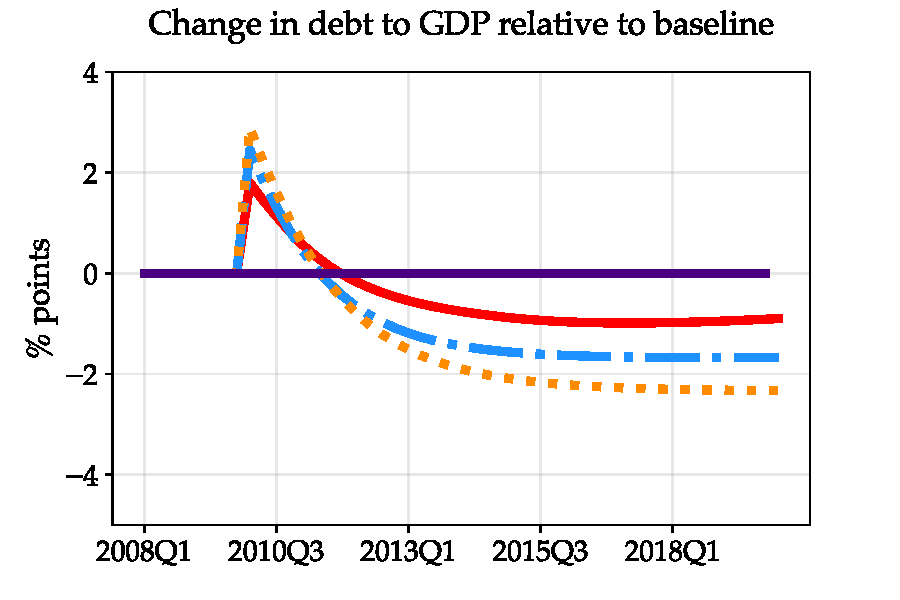
\includegraphics[scale=.57]{text/chapter1/Figures/Fiscal_Consolidation_CounterFactual/change_in_debt2GDP_CounterFactual_Fiscal_Consolidation_no_ZLB}
\label{fig:c}
\end{minipage}\hspace*{\fill}
\begin{minipage}{0.51\textwidth}
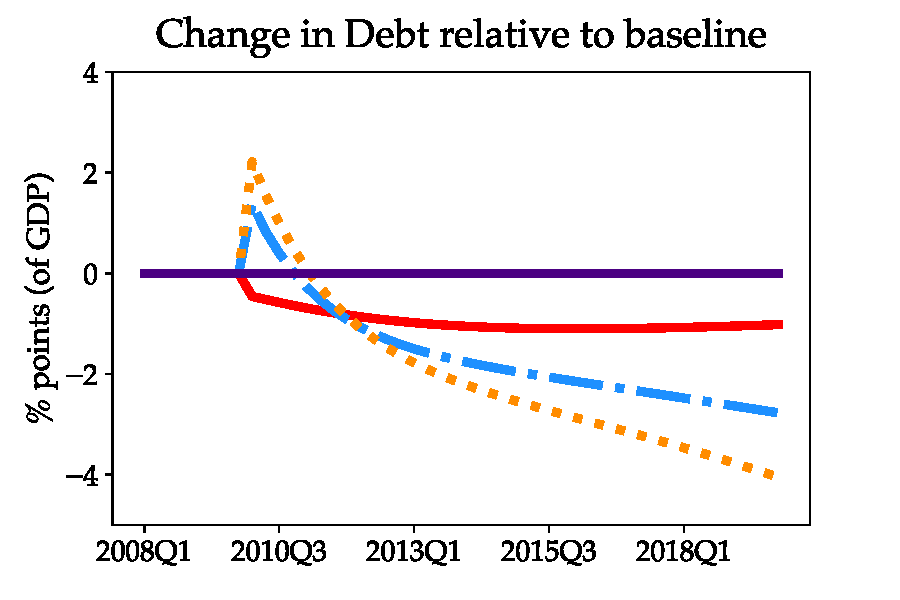
\includegraphics[scale=.57]{text/chapter1/Figures/Fiscal_Consolidation_CounterFactual/change_in_debt_CounterFactual_Fiscal_Consolidation_no_ZLB}
 \label{fig:d}
\end{minipage}


\caption{Counterfactual: Fiscal Consolidation in the US and the effects of the zero lower bound}
\label{FC_US_no_ZLB}
\end{figure}








% ----------------------------------------------------------------
\section{Conclusion}
% ----------------------------------------------------------------

This paper quantifies the macroeconomic role of a well-documented microeconomic fact, that job loss leads to scars on wages. Incorporating these microeconomic scars into a heterogeneous agent New Keynesian model with search and matching frictions introduces a novel channel that emerges as a key determinant of the speed of macroeconomic recovery from a recession. When estimated to match the microeconomic estimates on scarring, and calibrated to match the fraction of temporary layoffs in each recession, the model is able to quantitatively capture \textit{both} the sluggish recovery from the Great Recession and the swift rebound from the COVID Recession. During a recession, the extent to which micro unemployment scarring translates to macro scarring hinges on the share of temporary layoffs driving the rise in the unemployment rate. In particular, had the majority of layoffs during the COVID Recession been permanent rather than temporary, GDP would not have returned to its pre-2020 trend, even when accounting for the large fiscal response during the pandemic.

In addition, the transmission of fiscal austerity changes considerably in the presence of these scars. Given a reduction in government spending, scarring erodes future tax revenues, increasing pressure on the fiscal deficit. Quantitatively, the decline in debt to GDP from a fiscal consolidation is four times smaller because of unemployment scarring and leads to a near permanent rise in income inequality as scarring increases the dispersion in wages. 


The role of unemployment scarring in business cycle dynamics and macroeconomic policy presents many promising avenues for future research. First, the root causes of these scars remain an active area of research. Incorporating the origins of this microeconomic phenomenon into macroeconomic analysis could offer clearer guidance for designing policies to mitigate scarring. Additionally, the connection between unemployment scarring and sluggish recoveries highlights the potential of job retention schemes, like those implemented in Europe during the COVID recession, as an area for future research. As emphasized by \cite{Lachowska2020} and \cite{Jacobson1993}, "something intrinsic to the employment relationship itself... is lost when workers are displaced." Job retention policies may serve as the most effective hedge against scarring, given the inherent challenges of finding a strong employer-employee match. I leave these important questions for future research.





%\pagebreak 

% ----------------------------------------------------------------
\appendix
\setcounter{figure}{0} \renewcommand{\thefigure}{A.\arabic{figure}}
\setcounter{table}{0} \renewcommand{\thetable}{A.\arabic{table}}
\section{Additional Empirical Results}
\label{sec:appendix}
% ----------------------------------------------------------------


\subsection{Additional results with real-time forecasting of job risks}
\label{appendix:real_time_results_more}


Figure \ref{fig:real_time_ar} compares the real-time machine-efficient forecasts of job risks based on the Lasso with one from an AR(1) model using only the 3-month lag of the realized job flow rate. The two closely move with each other. The mean square errors (MSE) from the two are almost equal for both job finding and separation. This indicates that near-term job risks are highly predictable, especially in normal times. The major exceptions were during the Covid era. 

 \begin{figure}[ht]
    	\caption{Real-time Machine-efficient Risks from Lasso and AR(1)}
    	\label{fig:real_time_ar}
    	\begin{center}
	\adjustimage{max size={0.48\linewidth}}{Figures/predicted_comparison_JF_real_time_ar1.pdf} 
 	\adjustimage{max size={0.48\linewidth}}{Figures/predicted_comparison_JS_real_time_ar1.pdf} 
    	\end{center}
    	
    	\begin{flushleft}\footnotesize{Note: Multi-variate Lasso real-time forecasts versus one from AR(1) model.}\end{flushleft}
    \end{figure}


\subsection{Additional results with imputation of perceived job risks}



\subsubsection{Cross-validation of the imputing methodology}

We evaluate the performance of imputing methods used to backcast SCE job beliefs by examining if the imputed beliefs based on the 2013-2022 in-sample can successfully generate belief backcasts that match the observed expectations in MSC. In particular, Figure \ref{fig:impute_cv_with_msc_separation_inflation} plots the imputed beliefs for two series of expectations on median inflation expectations and 5-year-ahead job separation expectations in MSC based on 2013-2022 in-sample. They have an impressively large degree of comovement with the observed data. We are particularly careful to exclude any indices in MSC that are directly correlated to the target expectation series. They provide a strong external validation of our belief imputation methods. 

 \begin{figure}[ht]
    	\caption{Imputed Beliefs versus Observed Expectations in MSC}
    	\label{fig:impute_cv_with_msc_separation_inflation}
    	\begin{center}
\includegraphics[width=0.49\linewidth]{Figures/imputed_comparison_separation_5y_prob_msc_1step.pdf}  \includegraphics[width=0.49\linewidth]{Figures/imputed_comparison_inflation_msc_1step.pdf}  
    	\end{center}
    	
    	\begin{flushleft}Note: the figure plots the imputed beliefs from SCE regarding the percent chance the nationwide unemployment rate will be higher in the next year relative to the unemployment expectation index in MSC.\end{flushleft}
    \end{figure}



As a further validation of the imputation methodology across surveys, Figure \ref{fig:impute_cv_with_msc_ue} plots the imputed expectations in SCE regarding the median percent probability of nationwide unemployment rate to be higher, against the series of Michigan index regarding the direction of unemployment rate, which was observed for a much longer period. Again, in our in-sample Lasso imputation, we particularly exclude all Michigan indices regarding unemployment expectations to make it a fair test of the validity of our imputation methods. Because the SCE unemployment expectations are expressed as a percent probability while the MSC index is measured as the share of respondents expecting higher unemployment rates minus those expecting lower, we can not directly compare the imputation errors out-of-sample. We nevertheless show that the correlation between imputed expectations and the observed index in MSC is as high as 0.99. This suggests that our imputation method is able to do a great job of backcasting beliefs.   

 \begin{figure}[pt]
    	\caption{Imputed SCE versus Observed UE Expectations in MSC}
    	\label{fig:impute_cv_with_msc_ue}
    	\begin{center}
	\includegraphics[width=0.6\linewidth]{Figures/imputed_comparison_ue_prob_msc_1step.pdf} 
    	\end{center}
    	
    	\begin{flushleft}Note: the figure plots the imputed beliefs from SCE regarding the percent chance the nationwide unemployment rate will be higher in the next year relative to the unemployment expectation index in MSC.\end{flushleft}
    \end{figure}

\subsubsection{Hyper-parameter tuning of the Lasso model using cross-validation}

 Figure \ref{fig:impute_cv} plots the model score, i.e. out-of-sample average MSE from k-fold samples, under various values of $\alpha$. 

      \begin{figure}[ht]
    	\caption{Model Selection using Cross-Validation}
    	\label{fig:impute_cv}
    	\begin{center}
	\includegraphics[width=0.48\linewidth]{Figures/unbounded_imputing_job_finding_cv.pdf} 
\includegraphics[width=0.48\linewidth]{Figures/unbounded_imputing_job_separation_cv.pdf} 
    	\end{center}
    
    	\begin{flushleft}Note: mean square error scores under different penalization parameter $\alpha$ of the Lasso model.\end{flushleft}
    \end{figure}
    
\subsubsection{Inclusion of the pandemic era}
\label{appendix:sensitivity_imputation}

Figure \ref{fig:imputed_JF_comparison_covid} compares the imputed job risk belief relied upon pre-2020 sample as the in-sample of Lasso model with one relied on an extended sample covering the Covid era (2020-2022). The gap between the two series reveals a possible structural break in the relationship between job perceptions and other household expectations and macroeconomic conditions. However, such a different choice of in-sample period of the belief imputation does not significantly alter the patterns of the imputed out-of-sample job beliefs. The major exception was the job separation perceptions in the early 1980s.  

\begin{figure}[pt]
    \centering
    \caption{Imputing Beliefs Including or Excluding Covid Era}\label{fig:imputed_JF_comparison_covid}
\includegraphics[width=0.7\linewidth]{Figures/imputed_JF_comparison_covid.pdf} 
\includegraphics[width=0.7\linewidth]{Figures/imputed_JS_comparison_covid.pdf} 
\end{figure}

\subsubsection{Selected covariates of perceived risks}
\label{appendix: covariates_perceived_risks}

Figure \ref{fig:vars_rank} report the 10 most important variables selected from the Lasso model of imputation of perceived job risks, ranked by the absolute value of their estimated coefficients associated with the normalized value of each variable.  

    \begin{figure}[ht]
    	\caption{Selected variables of Lasso model of perceived job risks}
    	\label{fig:vars_rank}
    	\begin{center}
	\adjustimage{max size={0.48\linewidth}}{Figures/covariates_rank_job_finding.pdf} 
 	\adjustimage{max size={0.48\linewidth}}{Figures/covariates_rank_job_separation.pdf} 

    	\end{center}
    	
    	\begin{flushleft}\footnotesize{Note: selected variables ranked by the absolute value of their estimated coefficients in the Lasso imputation model for perceived job finding (left) and separation (right). The in-sample is between 2013-2020. UERate: real-time unemployment rate. Durrn\_gt\_all: good time to buy durables. Pexp\_f\_all: expecting better personal finance one year from now. Bus12\_f\_all: better nationwide business conditions a year from now. Px1\_15p\_all: expected inflation above 15 percent. Vehrn\_gt\_all: good time to buy vehicles. ptrd\_bb\_all: better off financially a year ago and better off a year from now. bago\_s\_all: same business conditions compared to a year ago. Pagorn\_hp\_all: worse financial situation than a year ago due to higher prices. Ptrd\_ss\_all: same personal finance compared to a year ago and will be the same a year from now. Pexp\_u\_all: worse personal finance one year from now. Newsrn\_u\_eng\_all: heard unfavorable news about the energy crisis. Newsrn\_u\_stk\_all: heard about unfavorable news regarding the stock market. Vehrn\_fb\_all: a bad time to buy vehicles due to uncertain future. Px1\_dkup\_all: do not know about future inflation. Newsrn\_u\_dem\_all: heard unfavorable news about lower consumer demand. INF\_Y2Y: real-time annual realized inflation rate. Bago\_f\_all: better business conditions compared to a year ago. Pagorn\_hd\_all: worse personal finance due to higher debt.}  \end{flushleft}
    \end{figure}

   \begin{figure}[ht]
    	\caption{Imputed job finding rate and realizations}
    	\label{fig:impute_comparison_1step}
    	\begin{center}
	\adjustimage{max size={0.7\linewidth}}{Figures/unbounded_imputed_comparison_1step_job_finding.pdf} \\
 	\adjustimage{max size={0.7\linewidth}}{Figures/unbounded_imputed_comparison_1step_job_separation.pdf}
    	\end{center}
    	\begin{flushleft}\footnotesize{Note: imputed perceived risks in the sample (2013-2022) and out-of-sample (1980-2013) compared to realized job flow rates.} \end{flushleft}
    \end{figure}


\subsubsection{Imputed beliefs by education group}

Figure \ref{fig:impute_by_education} plots the in-sample fitted and out-of-sample imputed perceptions of the job finding and separations rates for low, middle, and high education groups, versus the realized rates for each group. 

 \begin{figure}[pt]
    	\caption{Imputed beliefs by education}
    	\label{fig:impute_by_education}
    	\begin{center}
	\adjustimage{max size={0.43\linewidth}}{Figures/imputed_comparison_JF_LowEdu_1step.pdf}  
 	\adjustimage{max size={0.43\linewidth}}{Figures/imputed_comparison_JS_LowEdu_1step.pdf}  \\
 	\adjustimage{max size={0.43\linewidth}}{Figures/imputed_comparison_JF_MidEdu_1step.pdf} 	\adjustimage{max size={0.43\linewidth}}{Figures/imputed_comparison_JS_MidEdu_1step.pdf} \\
  	\adjustimage{max size={0.43\linewidth}}{Figures/imputed_comparison_JF_HighEdu_1step.pdf} 
    	\adjustimage{max size={0.43\linewidth}}{Figures/imputed_comparison_JS_HighEdu_1step.pdf} 
    	\end{center}
    	
    	\begin{flushleft}\footnotesize {Note: these figures plot the imputed perceived job separation and finding rates by low, middle and high educations, respectively, using the same methodology and the education-specific expectations in MSC.}\end{flushleft}
    \end{figure}

   

\subsection{Additional results with forecast errors}
\label{appendix:fe_results_more}

    The upper panel in Figure \ref{fig:forecast_errors} plots the FEs using two alternative series as realizations of job findings. During the majority of times in the sample, FEs lie in the negative domains, suggesting that on average, household beliefs underpredicted the realization of job-findings. This is consistent with the observation in Figure \ref{fig:impute_comparison_1step} that the imputed beliefs are below the realization most of the time. The periods with notable exceptions were the 1981-1982 recession and the Great Recession.
    
   
\begin{figure}[ht]
\caption{Forecast errors of job-finding and separation expectations}
\label{fig:forecast_errors}    
     	\begin{center}
 		%\adjustimage{max size={0.68\linewidth}}{Figures/forecast_errors.pdf} \\
 			\adjustimage{max size={0.8\linewidth}}{Figures/forecast_errors_size.pdf} %\\
    	\adjustimage{max size={0.8\linewidth}}{Figures/forecast_errors_size_job_separation.pdf} \\
 \end{center}
 \begin{flushleft}\footnotesize{Note: the absolute value of forecast errors of job finding and separation rates, defined as the difference both imputed/or observed perceived risk and the realized job transition rates.} \end{flushleft}
\end{figure}
    
    The lower panel plots the size of (absolute values) of the FEs. The size of FEs seemed to dramatically drop during recessions, compared to normal times. Some research has found that information-rigidity is counter-cyclical.\footnote{See \cite{coibion2015information} for the evidence with inflation expectations.}


\subsection{Additional evidence for the belief distortions over business cycles}

Instead of calculating peak-to-trough values of job risks as in Figure \ref{fig:bus_cycle_stats},  Figure \ref{fig:bus_cycle_stats_av} plots the average job finding/separation rates in normal times versus recessions and their average ratios, which show largely similar business cycle patterns of realized transition rates, risk forecasts and perceived job risks. 

\begin{figure}[pt] 
\centering 
	\caption{Business Cycle Patterns of Risks and Perceptions: Normal Times versus Recessions} 
	\label{fig:bus_cycle_stats_av}
\includegraphics[width=0.8\linewidth]{Figures/business_cycle_JF_stats.pdf} \\
\includegraphics[width=0.8\linewidth]{Figures/business_cycle_JS_stats.pdf} \\
    	\begin{flushleft}\footnotesize {Note: The left tables report the average perceived job risks, perceived job risks at different quantiles, real-time job risks, and realized job transition rates in normal times and NBER-labeled recessions. The right figures plot the ratio of these rates between recessions and normal times. The sample period is 1990-2024.} \end{flushleft}
\end{figure}



\section{Additional Model Results}
\label{appendix:model_results}

\input{model.tex}


\subsection{Details of the model experiments}

\subsubsection{Baseline model at the quarterly frequency}

The model experiments in Figure \ref{fig:pe_decompose_sub_obj} are based on directly estimated shocks to $JF$/$JS$, $\widetilde{JF}/\widetilde{JS}$ and ${JF}^*/{JS}^*$. To obtain such shocks, we estimate, respectively, a quarterly AR(1) model of each one of these sequences in the sample period up to the 2020 Q1. The predicted residuals are the estimated shocks to realized rates, beliefs, and rational job risk, which are plotted in Figure \ref{fig:shocks_from_data}. 

\begin{figure}[pt]
    \centering
    \caption{Shocks to realized job transitions, perceptions and rational forecasts}
    \label{fig:shocks_from_data} \includegraphics[width=0.45\linewidth]{Figures/estimated_shocks_job_finding.pdf}
    \includegraphics[width=0.45\linewidth]{Figures/estimated_shocks_job_separation.pdf}
\begin{flushleft}\footnotesize {Note: The figure plots the estimated shocks used for the experiments in Figure \ref{fig:pe_decompose_sub_obj}, based on an estimation of a quarterly AR(1) model on demeaned $JS_{t}\& JF_t$, $\widetilde{JS}_t \& \widetilde{JF}_t$, and $JS^{*}_t \& JF^{*}_t$. The sample period is between 1987 and 2020.} \end{flushleft}
\end{figure}


%\begin{figure}[pt]
%    \centering
%    \caption{Unemployment rate dynamics implied by the time paths of job finding and separation rates}
    %\label{fig:urate_model_data} \includegraphics[width=0.6\linewidth]{Figures/unemployment_rate_model_data.pdf}
%\begin{flushleft}\footnotesize {Note: The figure plots the simulated unemployment rate path based on the estimated shocks to realized $JS$ and $JF$ rates for the period 1988-2020. They are used for the experiments in Figure \ref{fig:pe_decompose_sub_obj}.} \end{flushleft}
%\end{figure}

Figure \ref{appendix_pe_decompose_sub_obj_educ} complements Figure \ref{fig:pe_decompose_sub_obj_educ} by showing the education-specific consumption aggregation fluctuations due to job separation and finding risks, separately. 

  \begin{figure}
        \centering
          \caption{Consumption Fluctuations due to JS and JF Risks: by Education}
\label{appendix_pe_decompose_sub_obj_educ}
\includegraphics[width=0.4\linewidth]{Figures/consumption_pe_JS_deviation_machine_as_rational_LowEdu.pdf}
\includegraphics[width=0.4\linewidth]{Figures/consumption_pe_JF_deviation_machine_as_rational_LowEdu.pdf}
%\includegraphics[width=0.6\linewidth]{Figures/consumption_pe_JS_JF_deviation_machine_as_rational_LowEdu.pdf} 
\\
\includegraphics[width=0.4\linewidth]{Figures/consumption_pe_JS_deviation_machine_as_rational_MidEdu.pdf}
\includegraphics[width=0.4\linewidth]{Figures/consumption_pe_JF_deviation_machine_as_rational_MidEdu.pdf}
%\includegraphics[width=0.6\linewidth]{Figures/consumption_pe_JS_JF_deviation_machine_as_rational_MidEdu.pdf}
\\

\includegraphics[width=0.4\linewidth]{Figures/consumption_pe_JS_deviation_machine_as_rational_HighEdu.pdf}
\includegraphics[width=0.4\linewidth]{Figures/consumption_pe_JF_deviation_machine_as_rational_HighEdu.pdf}
%\includegraphics[width=0.6\linewidth]{Figures/consumption_pe_JS_JF_deviation_machine_as_rational_HighEdu.pdf}
      \begin{flushleft}\footnotesize {Note: The figure compares for each education group their partial-equilibrium aggregate consumption deviations from its steady state simulated based on empirically estimated shocks to perceived job risk (subjective) and the real-time forecast risk (objective), in addition to the ex-post response to shocks to the realized job transition rates.} \end{flushleft}
    \end{figure}


\begin{center}\renewcommand{\arraystretch}{1.5}
\begin{table}
\centering
\caption{Household Calibration}\label{table:Calibration}
\makebox[\textwidth]{\begin{tabular}{|c|ccl|c|}
\hline
Description                     & \multicolumn{1}{c}{Parameter} & Value & \multicolumn{2}{c|}{Source/Target }\\ \hline
CRRA & \multicolumn{1}{c}{CRRA} & 2 & \multicolumn{2}{c|}{Standard} \\
Real Interest Rate                 & \multicolumn{1}{c}{$r$} & $1.03^{.25} - 1$ & \multicolumn{2}{c|}{ 3\% annualized real rate} \\
Probability of Death       & \multicolumn{1}{c}{$D$} & 0.00625 & \multicolumn{2}{c|}{\cite{carroll2017distribution}} \\
 \hline


UI replacement rate& \multicolumn{1}{c}{$\gamma$} & 0.5 & \multicolumn{2}{c|}{ 50$\%$ income drop at unemployment} \\
%Non UI income parameter 1 &  \multicolumn{1}{c}{$\gamma_{1}$} & 0.76 & \multicolumn{2}{c|}{ \cite{kekre2023unemployment} }\\
%Non UI income parameter 2 &  \multicolumn{1}{c}{$\gamma_{2}$} & 0.55 & \multicolumn{2}{c|}{\cite{kekre2023unemployment}} \\
%Gov. transfers &  \multicolumn{1}{c}{$T_{s}$} & 0.091 & \multicolumn{2}{c|}{\begin{footnotesize} $\frac{\text{SNAPS and Soc. Security Inc}}{\text{Pre Job Loss Income}} = .13$ \end{footnotesize}} \\
Std Dev of Log Permanent Shock  & \multicolumn{1}{c}{$\sigma_{\psi}$} & 0.06 & \multicolumn{2}{c|}{\cite{carroll2017distribution}} \\
Std Dev of Log Transitory Shock & \multicolumn{1}{c}{$\sigma_{\theta}$} & 0.2 & \multicolumn{2}{c|}{\cite{carroll2017distribution}} \\  \hline

Steady state Job Finding Rate & \multicolumn{1}{c}{$JF$} & 0.58 & \multicolumn{2}{c|}{CPS} \\ 
Steady state Job Separation Rate& \multicolumn{1}{c}{$JS$} & 0.070 & \multicolumn{2}{c|}{steady state unemployment rate=0.05} \\  \hline
Discount Factor & \multicolumn{1}{c}{$\beta$} &  0.976 & \multicolumn{2}{c|}{Quarterly MPC = 0.16} \\  \hline
\end{tabular}}
\end{table}
\end{center}



\subsubsection{Alternative model experiment at monthly frequency}

In this section, we report results from the baseline model experiments with a monthly version of the model with several modifications, which is calibrated similarly to \cite{kekre2023unemployment}. Since working with a quarterly model inevitably involves time-aggregation of monthly job flow rates and their belief counterparts, we see a monthly model as more robust to our assumptions on the time-aggregation. In particular, we replace the permanent wage component with a persistent component with a monthly AR(1) coefficient of 0.997, and a standard deviation of the shock of 0.057. We use steady-state monthly job finding rate to be 0.2517, the sample average from CPS before Covid era. 

Modifying the quarterly model assumption, we also assume that employment-to-unemployment transition is entirely driven by job separations, e.g.  $p(n_{i,t+1}=u|n_{i,t}=e) = JS_{t})$. We set its average to be 0.017. The discount factor beta is estimated to yield a quarterly MPC of 0.21, a la \cite{kekre2023unemployment}.  Figure \ref{fig:pe_decompose_sub_obj_monthly} shows the results with homogeneous workers, and Figure \ref{fig:pe_decompose_sub_obj_educ_monthly} shows that with heterogeneous risks by education.

\begin{figure}[ht]
    \centering
    \caption{\textbf{Monthly} Consumption Fluctuations due to Unemployment Risks}
    \label{fig:pe_decompose_sub_obj_monthly}

    \begin{subfigure}{0.32\linewidth}
         \caption*{Job separation}
        \includegraphics[width=\linewidth]{Figures/consumption_pe_JS_deviation_machine_as_rational_monthly.pdf}
   
    \end{subfigure}
    \hfill
    \begin{subfigure}{0.32\linewidth}
         \caption*{Job finding}
        \includegraphics[width=\linewidth]{Figures/consumption_pe_JF_deviation_machine_as_rational_monthly.pdf}
   
    \end{subfigure}
    \hfill
    \begin{subfigure}{0.32\linewidth}
         \caption*{Combined}
        \includegraphics[width=\linewidth]{Figures/consumption_pe_JS_JF_deviation_machine_as_rational_monthly.pdf}
   
    \end{subfigure}

    \begin{flushleft}
        \footnotesize 
        Note: The figure compares the partial-equilibrium aggregate consumption deviations from its steady state simulated based on empirically estimated shocks to perceived job risk (subjective) and the real-time forecast risk (objective), in addition to the ex-post response to shocks to the realized job transition rates. The results are from a monthly variation of the baseline model set at the quarterly frequency.
    \end{flushleft}
\end{figure}

  \begin{figure}[ht]
    \centering
    \caption{\textbf{Monthly} Consumption Fluctuations due to Unemployment Risks: by Education}
    \label{fig:pe_decompose_sub_obj_educ_monthly}

    \begin{subfigure}{0.32\linewidth}
     \caption*{Low Education}
        \includegraphics[width=\linewidth]{Figures/consumption_pe_JS_JF_deviation_machine_as_rational_LowEdu_monthly.pdf}
       
    \end{subfigure}
    \hfill
    \begin{subfigure}{0.32\linewidth}
     \caption*{Middle Education}
        \includegraphics[width=\linewidth]{Figures/consumption_pe_JS_JF_deviation_machine_as_rational_MidEdu_monthly.pdf}
       
    \end{subfigure}
    \hfill
    \begin{subfigure}{0.32\linewidth}
      \caption*{High Education}
        \includegraphics[width=\linewidth]{Figures/consumption_pe_JS_JF_deviation_machine_as_rational_HighEdu_monthly.pdf}
      
    \end{subfigure}

    \begin{flushleft}
        \footnotesize 
        Note: The figure compares for each education group their partial-equilibrium aggregate consumption deviations from its steady state simulated based on empirically estimated shocks to perceived job risk (subjective) and the real-time forecast risk (objective), in addition to the ex-post response to shocks to the realized job transition rates. The results are from the monthly version of the baseline model with modified assumptions.
    \end{flushleft}
\end{figure}

%\bibliography{PIR.bib}
%\bibliographystyle{apalike}

%\pagebreak 

% ----------------------------------------------------------------
\appendix
\setcounter{figure}{0} \renewcommand{\thefigure}{A.\arabic{figure}}
\setcounter{table}{0} \renewcommand{\thetable}{A.\arabic{table}}
\section{Additional Empirical Results}
\label{sec:appendix}
% ----------------------------------------------------------------


\subsection{Additional results with real-time forecasting of job risks}
\label{appendix:real_time_results_more}


Figure \ref{fig:real_time_ar} compares the real-time machine-efficient forecasts of job risks based on the Lasso with one from an AR(1) model using only the 3-month lag of the realized job flow rate. The two closely move with each other. The mean square errors (MSE) from the two are almost equal for both job finding and separation. This indicates that near-term job risks are highly predictable, especially in normal times. The major exceptions were during the Covid era. 

 \begin{figure}[ht]
    	\caption{Real-time Machine-efficient Risks from Lasso and AR(1)}
    	\label{fig:real_time_ar}
    	\begin{center}
	\adjustimage{max size={0.48\linewidth}}{Figures/predicted_comparison_JF_real_time_ar1.pdf} 
 	\adjustimage{max size={0.48\linewidth}}{Figures/predicted_comparison_JS_real_time_ar1.pdf} 
    	\end{center}
    	
    	\begin{flushleft}\footnotesize{Note: Multi-variate Lasso real-time forecasts versus one from AR(1) model.}\end{flushleft}
    \end{figure}


\subsection{Additional results with imputation of perceived job risks}



\subsubsection{Cross-validation of the imputing methodology}

We evaluate the performance of imputing methods used to backcast SCE job beliefs by examining if the imputed beliefs based on the 2013-2022 in-sample can successfully generate belief backcasts that match the observed expectations in MSC. In particular, Figure \ref{fig:impute_cv_with_msc_separation_inflation} plots the imputed beliefs for two series of expectations on median inflation expectations and 5-year-ahead job separation expectations in MSC based on 2013-2022 in-sample. They have an impressively large degree of comovement with the observed data. We are particularly careful to exclude any indices in MSC that are directly correlated to the target expectation series. They provide a strong external validation of our belief imputation methods. 

 \begin{figure}[ht]
    	\caption{Imputed Beliefs versus Observed Expectations in MSC}
    	\label{fig:impute_cv_with_msc_separation_inflation}
    	\begin{center}
\includegraphics[width=0.49\linewidth]{Figures/imputed_comparison_separation_5y_prob_msc_1step.pdf}  \includegraphics[width=0.49\linewidth]{Figures/imputed_comparison_inflation_msc_1step.pdf}  
    	\end{center}
    	
    	\begin{flushleft}Note: the figure plots the imputed beliefs from SCE regarding the percent chance the nationwide unemployment rate will be higher in the next year relative to the unemployment expectation index in MSC.\end{flushleft}
    \end{figure}



As a further validation of the imputation methodology across surveys, Figure \ref{fig:impute_cv_with_msc_ue} plots the imputed expectations in SCE regarding the median percent probability of nationwide unemployment rate to be higher, against the series of Michigan index regarding the direction of unemployment rate, which was observed for a much longer period. Again, in our in-sample Lasso imputation, we particularly exclude all Michigan indices regarding unemployment expectations to make it a fair test of the validity of our imputation methods. Because the SCE unemployment expectations are expressed as a percent probability while the MSC index is measured as the share of respondents expecting higher unemployment rates minus those expecting lower, we can not directly compare the imputation errors out-of-sample. We nevertheless show that the correlation between imputed expectations and the observed index in MSC is as high as 0.99. This suggests that our imputation method is able to do a great job of backcasting beliefs.   

 \begin{figure}[pt]
    	\caption{Imputed SCE versus Observed UE Expectations in MSC}
    	\label{fig:impute_cv_with_msc_ue}
    	\begin{center}
	\includegraphics[width=0.6\linewidth]{Figures/imputed_comparison_ue_prob_msc_1step.pdf} 
    	\end{center}
    	
    	\begin{flushleft}Note: the figure plots the imputed beliefs from SCE regarding the percent chance the nationwide unemployment rate will be higher in the next year relative to the unemployment expectation index in MSC.\end{flushleft}
    \end{figure}

\subsubsection{Hyper-parameter tuning of the Lasso model using cross-validation}

 Figure \ref{fig:impute_cv} plots the model score, i.e. out-of-sample average MSE from k-fold samples, under various values of $\alpha$. 

      \begin{figure}[ht]
    	\caption{Model Selection using Cross-Validation}
    	\label{fig:impute_cv}
    	\begin{center}
	\includegraphics[width=0.48\linewidth]{Figures/unbounded_imputing_job_finding_cv.pdf} 
\includegraphics[width=0.48\linewidth]{Figures/unbounded_imputing_job_separation_cv.pdf} 
    	\end{center}
    
    	\begin{flushleft}Note: mean square error scores under different penalization parameter $\alpha$ of the Lasso model.\end{flushleft}
    \end{figure}
    
\subsubsection{Inclusion of the pandemic era}
\label{appendix:sensitivity_imputation}

Figure \ref{fig:imputed_JF_comparison_covid} compares the imputed job risk belief relied upon pre-2020 sample as the in-sample of Lasso model with one relied on an extended sample covering the Covid era (2020-2022). The gap between the two series reveals a possible structural break in the relationship between job perceptions and other household expectations and macroeconomic conditions. However, such a different choice of in-sample period of the belief imputation does not significantly alter the patterns of the imputed out-of-sample job beliefs. The major exception was the job separation perceptions in the early 1980s.  

\begin{figure}[pt]
    \centering
    \caption{Imputing Beliefs Including or Excluding Covid Era}\label{fig:imputed_JF_comparison_covid}
\includegraphics[width=0.7\linewidth]{Figures/imputed_JF_comparison_covid.pdf} 
\includegraphics[width=0.7\linewidth]{Figures/imputed_JS_comparison_covid.pdf} 
\end{figure}

\subsubsection{Selected covariates of perceived risks}
\label{appendix: covariates_perceived_risks}

Figure \ref{fig:vars_rank} report the 10 most important variables selected from the Lasso model of imputation of perceived job risks, ranked by the absolute value of their estimated coefficients associated with the normalized value of each variable.  

    \begin{figure}[ht]
    	\caption{Selected variables of Lasso model of perceived job risks}
    	\label{fig:vars_rank}
    	\begin{center}
	\adjustimage{max size={0.48\linewidth}}{Figures/covariates_rank_job_finding.pdf} 
 	\adjustimage{max size={0.48\linewidth}}{Figures/covariates_rank_job_separation.pdf} 

    	\end{center}
    	
    	\begin{flushleft}\footnotesize{Note: selected variables ranked by the absolute value of their estimated coefficients in the Lasso imputation model for perceived job finding (left) and separation (right). The in-sample is between 2013-2020. UERate: real-time unemployment rate. Durrn\_gt\_all: good time to buy durables. Pexp\_f\_all: expecting better personal finance one year from now. Bus12\_f\_all: better nationwide business conditions a year from now. Px1\_15p\_all: expected inflation above 15 percent. Vehrn\_gt\_all: good time to buy vehicles. ptrd\_bb\_all: better off financially a year ago and better off a year from now. bago\_s\_all: same business conditions compared to a year ago. Pagorn\_hp\_all: worse financial situation than a year ago due to higher prices. Ptrd\_ss\_all: same personal finance compared to a year ago and will be the same a year from now. Pexp\_u\_all: worse personal finance one year from now. Newsrn\_u\_eng\_all: heard unfavorable news about the energy crisis. Newsrn\_u\_stk\_all: heard about unfavorable news regarding the stock market. Vehrn\_fb\_all: a bad time to buy vehicles due to uncertain future. Px1\_dkup\_all: do not know about future inflation. Newsrn\_u\_dem\_all: heard unfavorable news about lower consumer demand. INF\_Y2Y: real-time annual realized inflation rate. Bago\_f\_all: better business conditions compared to a year ago. Pagorn\_hd\_all: worse personal finance due to higher debt.}  \end{flushleft}
    \end{figure}

   \begin{figure}[ht]
    	\caption{Imputed job finding rate and realizations}
    	\label{fig:impute_comparison_1step}
    	\begin{center}
	\adjustimage{max size={0.7\linewidth}}{Figures/unbounded_imputed_comparison_1step_job_finding.pdf} \\
 	\adjustimage{max size={0.7\linewidth}}{Figures/unbounded_imputed_comparison_1step_job_separation.pdf}
    	\end{center}
    	\begin{flushleft}\footnotesize{Note: imputed perceived risks in the sample (2013-2022) and out-of-sample (1980-2013) compared to realized job flow rates.} \end{flushleft}
    \end{figure}


\subsubsection{Imputed beliefs by education group}

Figure \ref{fig:impute_by_education} plots the in-sample fitted and out-of-sample imputed perceptions of the job finding and separations rates for low, middle, and high education groups, versus the realized rates for each group. 

 \begin{figure}[pt]
    	\caption{Imputed beliefs by education}
    	\label{fig:impute_by_education}
    	\begin{center}
	\adjustimage{max size={0.43\linewidth}}{Figures/imputed_comparison_JF_LowEdu_1step.pdf}  
 	\adjustimage{max size={0.43\linewidth}}{Figures/imputed_comparison_JS_LowEdu_1step.pdf}  \\
 	\adjustimage{max size={0.43\linewidth}}{Figures/imputed_comparison_JF_MidEdu_1step.pdf} 	\adjustimage{max size={0.43\linewidth}}{Figures/imputed_comparison_JS_MidEdu_1step.pdf} \\
  	\adjustimage{max size={0.43\linewidth}}{Figures/imputed_comparison_JF_HighEdu_1step.pdf} 
    	\adjustimage{max size={0.43\linewidth}}{Figures/imputed_comparison_JS_HighEdu_1step.pdf} 
    	\end{center}
    	
    	\begin{flushleft}\footnotesize {Note: these figures plot the imputed perceived job separation and finding rates by low, middle and high educations, respectively, using the same methodology and the education-specific expectations in MSC.}\end{flushleft}
    \end{figure}

   

\subsection{Additional results with forecast errors}
\label{appendix:fe_results_more}

    The upper panel in Figure \ref{fig:forecast_errors} plots the FEs using two alternative series as realizations of job findings. During the majority of times in the sample, FEs lie in the negative domains, suggesting that on average, household beliefs underpredicted the realization of job-findings. This is consistent with the observation in Figure \ref{fig:impute_comparison_1step} that the imputed beliefs are below the realization most of the time. The periods with notable exceptions were the 1981-1982 recession and the Great Recession.
    
   
\begin{figure}[ht]
\caption{Forecast errors of job-finding and separation expectations}
\label{fig:forecast_errors}    
     	\begin{center}
 		%\adjustimage{max size={0.68\linewidth}}{Figures/forecast_errors.pdf} \\
 			\adjustimage{max size={0.8\linewidth}}{Figures/forecast_errors_size.pdf} %\\
    	\adjustimage{max size={0.8\linewidth}}{Figures/forecast_errors_size_job_separation.pdf} \\
 \end{center}
 \begin{flushleft}\footnotesize{Note: the absolute value of forecast errors of job finding and separation rates, defined as the difference both imputed/or observed perceived risk and the realized job transition rates.} \end{flushleft}
\end{figure}
    
    The lower panel plots the size of (absolute values) of the FEs. The size of FEs seemed to dramatically drop during recessions, compared to normal times. Some research has found that information-rigidity is counter-cyclical.\footnote{See \cite{coibion2015information} for the evidence with inflation expectations.}


\subsection{Additional evidence for the belief distortions over business cycles}

Instead of calculating peak-to-trough values of job risks as in Figure \ref{fig:bus_cycle_stats},  Figure \ref{fig:bus_cycle_stats_av} plots the average job finding/separation rates in normal times versus recessions and their average ratios, which show largely similar business cycle patterns of realized transition rates, risk forecasts and perceived job risks. 

\begin{figure}[pt] 
\centering 
	\caption{Business Cycle Patterns of Risks and Perceptions: Normal Times versus Recessions} 
	\label{fig:bus_cycle_stats_av}
\includegraphics[width=0.8\linewidth]{Figures/business_cycle_JF_stats.pdf} \\
\includegraphics[width=0.8\linewidth]{Figures/business_cycle_JS_stats.pdf} \\
    	\begin{flushleft}\footnotesize {Note: The left tables report the average perceived job risks, perceived job risks at different quantiles, real-time job risks, and realized job transition rates in normal times and NBER-labeled recessions. The right figures plot the ratio of these rates between recessions and normal times. The sample period is 1990-2024.} \end{flushleft}
\end{figure}



\section{Additional Model Results}
\label{appendix:model_results}

\input{model.tex}


\subsection{Details of the model experiments}

\subsubsection{Baseline model at the quarterly frequency}

The model experiments in Figure \ref{fig:pe_decompose_sub_obj} are based on directly estimated shocks to $JF$/$JS$, $\widetilde{JF}/\widetilde{JS}$ and ${JF}^*/{JS}^*$. To obtain such shocks, we estimate, respectively, a quarterly AR(1) model of each one of these sequences in the sample period up to the 2020 Q1. The predicted residuals are the estimated shocks to realized rates, beliefs, and rational job risk, which are plotted in Figure \ref{fig:shocks_from_data}. 

\begin{figure}[pt]
    \centering
    \caption{Shocks to realized job transitions, perceptions and rational forecasts}
    \label{fig:shocks_from_data} \includegraphics[width=0.45\linewidth]{Figures/estimated_shocks_job_finding.pdf}
    \includegraphics[width=0.45\linewidth]{Figures/estimated_shocks_job_separation.pdf}
\begin{flushleft}\footnotesize {Note: The figure plots the estimated shocks used for the experiments in Figure \ref{fig:pe_decompose_sub_obj}, based on an estimation of a quarterly AR(1) model on demeaned $JS_{t}\& JF_t$, $\widetilde{JS}_t \& \widetilde{JF}_t$, and $JS^{*}_t \& JF^{*}_t$. The sample period is between 1987 and 2020.} \end{flushleft}
\end{figure}


%\begin{figure}[pt]
%    \centering
%    \caption{Unemployment rate dynamics implied by the time paths of job finding and separation rates}
    %\label{fig:urate_model_data} \includegraphics[width=0.6\linewidth]{Figures/unemployment_rate_model_data.pdf}
%\begin{flushleft}\footnotesize {Note: The figure plots the simulated unemployment rate path based on the estimated shocks to realized $JS$ and $JF$ rates for the period 1988-2020. They are used for the experiments in Figure \ref{fig:pe_decompose_sub_obj}.} \end{flushleft}
%\end{figure}

Figure \ref{appendix_pe_decompose_sub_obj_educ} complements Figure \ref{fig:pe_decompose_sub_obj_educ} by showing the education-specific consumption aggregation fluctuations due to job separation and finding risks, separately. 

  \begin{figure}
        \centering
          \caption{Consumption Fluctuations due to JS and JF Risks: by Education}
\label{appendix_pe_decompose_sub_obj_educ}
\includegraphics[width=0.4\linewidth]{Figures/consumption_pe_JS_deviation_machine_as_rational_LowEdu.pdf}
\includegraphics[width=0.4\linewidth]{Figures/consumption_pe_JF_deviation_machine_as_rational_LowEdu.pdf}
%\includegraphics[width=0.6\linewidth]{Figures/consumption_pe_JS_JF_deviation_machine_as_rational_LowEdu.pdf} 
\\
\includegraphics[width=0.4\linewidth]{Figures/consumption_pe_JS_deviation_machine_as_rational_MidEdu.pdf}
\includegraphics[width=0.4\linewidth]{Figures/consumption_pe_JF_deviation_machine_as_rational_MidEdu.pdf}
%\includegraphics[width=0.6\linewidth]{Figures/consumption_pe_JS_JF_deviation_machine_as_rational_MidEdu.pdf}
\\

\includegraphics[width=0.4\linewidth]{Figures/consumption_pe_JS_deviation_machine_as_rational_HighEdu.pdf}
\includegraphics[width=0.4\linewidth]{Figures/consumption_pe_JF_deviation_machine_as_rational_HighEdu.pdf}
%\includegraphics[width=0.6\linewidth]{Figures/consumption_pe_JS_JF_deviation_machine_as_rational_HighEdu.pdf}
      \begin{flushleft}\footnotesize {Note: The figure compares for each education group their partial-equilibrium aggregate consumption deviations from its steady state simulated based on empirically estimated shocks to perceived job risk (subjective) and the real-time forecast risk (objective), in addition to the ex-post response to shocks to the realized job transition rates.} \end{flushleft}
    \end{figure}


\begin{center}\renewcommand{\arraystretch}{1.5}
\begin{table}
\centering
\caption{Household Calibration}\label{table:Calibration}
\makebox[\textwidth]{\begin{tabular}{|c|ccl|c|}
\hline
Description                     & \multicolumn{1}{c}{Parameter} & Value & \multicolumn{2}{c|}{Source/Target }\\ \hline
CRRA & \multicolumn{1}{c}{CRRA} & 2 & \multicolumn{2}{c|}{Standard} \\
Real Interest Rate                 & \multicolumn{1}{c}{$r$} & $1.03^{.25} - 1$ & \multicolumn{2}{c|}{ 3\% annualized real rate} \\
Probability of Death       & \multicolumn{1}{c}{$D$} & 0.00625 & \multicolumn{2}{c|}{\cite{carroll2017distribution}} \\
 \hline


UI replacement rate& \multicolumn{1}{c}{$\gamma$} & 0.5 & \multicolumn{2}{c|}{ 50$\%$ income drop at unemployment} \\
%Non UI income parameter 1 &  \multicolumn{1}{c}{$\gamma_{1}$} & 0.76 & \multicolumn{2}{c|}{ \cite{kekre2023unemployment} }\\
%Non UI income parameter 2 &  \multicolumn{1}{c}{$\gamma_{2}$} & 0.55 & \multicolumn{2}{c|}{\cite{kekre2023unemployment}} \\
%Gov. transfers &  \multicolumn{1}{c}{$T_{s}$} & 0.091 & \multicolumn{2}{c|}{\begin{footnotesize} $\frac{\text{SNAPS and Soc. Security Inc}}{\text{Pre Job Loss Income}} = .13$ \end{footnotesize}} \\
Std Dev of Log Permanent Shock  & \multicolumn{1}{c}{$\sigma_{\psi}$} & 0.06 & \multicolumn{2}{c|}{\cite{carroll2017distribution}} \\
Std Dev of Log Transitory Shock & \multicolumn{1}{c}{$\sigma_{\theta}$} & 0.2 & \multicolumn{2}{c|}{\cite{carroll2017distribution}} \\  \hline

Steady state Job Finding Rate & \multicolumn{1}{c}{$JF$} & 0.58 & \multicolumn{2}{c|}{CPS} \\ 
Steady state Job Separation Rate& \multicolumn{1}{c}{$JS$} & 0.070 & \multicolumn{2}{c|}{steady state unemployment rate=0.05} \\  \hline
Discount Factor & \multicolumn{1}{c}{$\beta$} &  0.976 & \multicolumn{2}{c|}{Quarterly MPC = 0.16} \\  \hline
\end{tabular}}
\end{table}
\end{center}



\subsubsection{Alternative model experiment at monthly frequency}

In this section, we report results from the baseline model experiments with a monthly version of the model with several modifications, which is calibrated similarly to \cite{kekre2023unemployment}. Since working with a quarterly model inevitably involves time-aggregation of monthly job flow rates and their belief counterparts, we see a monthly model as more robust to our assumptions on the time-aggregation. In particular, we replace the permanent wage component with a persistent component with a monthly AR(1) coefficient of 0.997, and a standard deviation of the shock of 0.057. We use steady-state monthly job finding rate to be 0.2517, the sample average from CPS before Covid era. 

Modifying the quarterly model assumption, we also assume that employment-to-unemployment transition is entirely driven by job separations, e.g.  $p(n_{i,t+1}=u|n_{i,t}=e) = JS_{t})$. We set its average to be 0.017. The discount factor beta is estimated to yield a quarterly MPC of 0.21, a la \cite{kekre2023unemployment}.  Figure \ref{fig:pe_decompose_sub_obj_monthly} shows the results with homogeneous workers, and Figure \ref{fig:pe_decompose_sub_obj_educ_monthly} shows that with heterogeneous risks by education.

\begin{figure}[ht]
    \centering
    \caption{\textbf{Monthly} Consumption Fluctuations due to Unemployment Risks}
    \label{fig:pe_decompose_sub_obj_monthly}

    \begin{subfigure}{0.32\linewidth}
         \caption*{Job separation}
        \includegraphics[width=\linewidth]{Figures/consumption_pe_JS_deviation_machine_as_rational_monthly.pdf}
   
    \end{subfigure}
    \hfill
    \begin{subfigure}{0.32\linewidth}
         \caption*{Job finding}
        \includegraphics[width=\linewidth]{Figures/consumption_pe_JF_deviation_machine_as_rational_monthly.pdf}
   
    \end{subfigure}
    \hfill
    \begin{subfigure}{0.32\linewidth}
         \caption*{Combined}
        \includegraphics[width=\linewidth]{Figures/consumption_pe_JS_JF_deviation_machine_as_rational_monthly.pdf}
   
    \end{subfigure}

    \begin{flushleft}
        \footnotesize 
        Note: The figure compares the partial-equilibrium aggregate consumption deviations from its steady state simulated based on empirically estimated shocks to perceived job risk (subjective) and the real-time forecast risk (objective), in addition to the ex-post response to shocks to the realized job transition rates. The results are from a monthly variation of the baseline model set at the quarterly frequency.
    \end{flushleft}
\end{figure}

  \begin{figure}[ht]
    \centering
    \caption{\textbf{Monthly} Consumption Fluctuations due to Unemployment Risks: by Education}
    \label{fig:pe_decompose_sub_obj_educ_monthly}

    \begin{subfigure}{0.32\linewidth}
     \caption*{Low Education}
        \includegraphics[width=\linewidth]{Figures/consumption_pe_JS_JF_deviation_machine_as_rational_LowEdu_monthly.pdf}
       
    \end{subfigure}
    \hfill
    \begin{subfigure}{0.32\linewidth}
     \caption*{Middle Education}
        \includegraphics[width=\linewidth]{Figures/consumption_pe_JS_JF_deviation_machine_as_rational_MidEdu_monthly.pdf}
       
    \end{subfigure}
    \hfill
    \begin{subfigure}{0.32\linewidth}
      \caption*{High Education}
        \includegraphics[width=\linewidth]{Figures/consumption_pe_JS_JF_deviation_machine_as_rational_HighEdu_monthly.pdf}
      
    \end{subfigure}

    \begin{flushleft}
        \footnotesize 
        Note: The figure compares for each education group their partial-equilibrium aggregate consumption deviations from its steady state simulated based on empirically estimated shocks to perceived job risk (subjective) and the real-time forecast risk (objective), in addition to the ex-post response to shocks to the realized job transition rates. The results are from the monthly version of the baseline model with modified assumptions.
    \end{flushleft}
\end{figure}

%\end{document}


%\printbibliography[title=References]}
%\end{refsection}
%
%\begin{refsection}[myrefs.bib]
%\chapter[The Macroeconomic Consequences of Unemployment Scarring]
\chapter[Perceived Unemployment Risks over Business Cycles]{Perceived Unemployment Risks over Business Cycles\raisebox{.3\baselineskip}{\normalsize\footnotemark}}
%\footnotetext{}
%\label{chap1}
\begin{flushright}
{\large -- joint with Adrian Monninger, Xincheng Qiu, and Tao Wang}\end{flushright} %


\begin{titlepage}
	\title{\textbf{The Macroeconomic Consequences of Unemployment Scarring}  % \\ \textcolor{red}{PRELIMINARY AND INCOMPLETE}
		\author{
	William Du\thanks{ Johns Hopkins University, Department of Economics, 3100 Wyman Park Drive, Baltimore, MD 21211.
E-mail: \href{wdu9@jhu.edu}{wdu9@jhu.edu}. I am deeply indebted to Christopher Carroll, Jonathan Wright, and Francesco Bianchi for their guidance and support in the development of this paper. For their helpful comments, I thank Mateo Vel\'{a}squez-Giraldo, Wonsik Ko, Bence Bard\'{o}czy, Jeongwon Son, John Green, Tao Wang, Laurence Ball, Greg Duffee, Robert Moffitt, Xincheng Qiu, Yucheng Yang, Jeffrey Sun, Sebastian Graves,  Adrian Monninger, Jamie Lenney, and Kyung Woong Koh. Finally, I thank participants at the 2024 IAAE annual conference and 2024 SCE annual conference. }} \\ \text{\begin{large}Johns Hopkins University \end{large}}}
	\date{\today }
	\maketitle
	\begin{abstract}
	\begin{singlespace}
		\noindent  Job loss leaves scars on wages that persist for more than 20 years. Yet, the importance of this well-documented micro fact for macro dynamics remains largely unexplored. This paper argues that these scars are a key determinant of the speed of macroeconomic recovery following recessions. I incorporate human capital into a heterogeneous agent New Keynesian (HANK) model with search and matching frictions. During unemployment, human capital depreciates, leading to lower wages for reemployed workers. Unemployment scarring, mediated by the fraction of temporary versus permanent layoffs, enables the model to capture \textit{both} the sluggish recovery from the Great Recession and the rapid rebound from the COVID Recession. In particular, the presence of scarring reveals the pivotal role that temporary layoffs fulfilled in supporting the swift post-pandemic recovery and in preventing a subsequent permanent rise in inequality. In a counterfactual analysis of the Great Recession, a U.S. fiscal consolidation would have proven substantially less effective at reducing debt-to-GDP as scarring erodes future tax revenues and therefore increases pressure on the fiscal deficit.

  
\end{singlespace}
\medskip
	
	\end{abstract}

\end{titlepage}




% ----------------------------------------------------------------
\section{Introduction}
% ----------------------------------------------------------------
Since the seminal work of \cite{Jacobson1993}, job loss from stable employment has been understood to cause large and persistent earnings losses.\footnote{In the microeconomic literature, these losses apply to workers who have been employed for 3 to 10 years.} On average, these earnings losses are 15$\%$ after 20 years \citep[e.g.][]{DavisVonWachter2011, Huckfeldt2022}, reflect a permanent loss in wages as opposed to hours \citep[e.g.][]{Moore2019, Lachowska2020,Huckfeldt2022}, worsen in recessions \citep{DavisVonWachter2011, Schmieder2023}, and are concentrated among workers who switch into lower paying occupations \citep{Huckfeldt2022}.\footnote{\cite{Huckfeldt2022} and \cite{Fujita2017} document that over $50\%$ of the unemployed switch occupations. } While a growing \textit{microeconomic} literature seeks to explain the origins of these `scars', few \textit{macroeconomic} papers explore whether these scars matter \textit{quantitatively} for business cycle dynamics, fiscal policy, and monetary policy. The thesis of this paper is that these microeconomic scars are a key determinant of the speed of macroeconomic recovery from recessions.


To quantify the macroeconomic role of microeconomic unemployment scarring, I extend a heterogeneous agent New Keynesian (HANK) model with search and matching (SAM) frictions to include human capital dynamics. In the model, households make a consumption/saving decision in the face of unemployment risk and search frictions in the labor market. To account for the empirical fact that only workers who are permanently laid off suffer from scarring \citep{ Fujita2016}, \footnote{A permanent layoff refers to a worker who has been permanently separated from their previous employer.} the model differentiates between permanent layoffs, temporary layoffs, and other types of unemployment. Temporary layoffs can transition to permanent layoffs and, motivated by recent evidence using U.S. that suggests these scars reflect a loss in productivity \footnote{ The current literature suggests that,in the U.S., the these scars are largely due to losses in firm specific human capital. To begin, \cite{Lachowska2020} find that the decline in wages is largely explained by losses in match specific productivity. \cite{Poletaev2008} find that reemployed workers who suffer large wage losses employ substantially different skills in their new job. \cite{Huckfeldt2022} documents that scarring is concentrated among workers who switch into lower paying occupations.}, only households who find reemployment after a permanent layoff spell \textit{may} experience human capital depreciation.The model does not capture the sources that lead firms to engage in temporary layoffs. Instead, using the estimates from \cite{Gertler2022}, the unemployment process across different layoff states is calibrated to match \textit{how} each state evolves during recessions.%\footnote{ Unsurprisingly, \cite{Fujita2016} documents that temporary layoffs in the Current Population Survey "earn about the same income as before (job loss)". } \cite{Arash2015} document in Austrian Administrative data that workers who are recalled experience a slight increase in wages. Finally, in a sample of UI recipients from Missouri and Pennsylvania in the 1980s, \cite{Katz1990} find that, on average, there is a $1.4\%$ decline in hourly earnings for workers who are recalled to their previous employer.} 

I begin by showing that when the model accounts for the microeconomic estimates of unemployment scarring from \cite{DavisVonWachter2011}, the resulting decline in macroeconomic activity is sufficiently persistent to validate unemployment scarring as a new microfoundation for hysteresis and endogenous growth. In particular, with scarring, recessions induce a near-permanent decline in output, consumption, and aggregate labor productivity. Furthermore, since these scars arise from a loss of human capital that reduces both labor income and productivity, the persistent decline in macroeconomic activity occurs without a sustained rise in the unemployment rate. In addition, unemployment scarring induces a permanent increase in wage dispersion that results in a lasting increase in income inequality, a result supported by the data but unaccounted for in standard models of hysteresis or endogenous growth. Finally, the near-permanent decline in wages caused by scarring reduces future tax revenues, increasing the pressure that recessions place on the fiscal deficit since losses in tax revenues necessitate a larger increase in debt to sustain government expenditures. 


 Having shown that scarring induces large and persistent declines in macroeconomic activity, I then demonstrate that unemployment scarring, when disciplined by the microeconomic evidence, explains a substantial portion of the sluggish recovery from the Great Recession, a challenging feat that can only be accomplished by a model that can generate a decline in income that is more persistent than the increase in the unemployment rate. To do so, I simulate the model to replicate the path of unemployment from 2008 to 2019 and then compare the untargeted paths of consumption and output against the data. The goal of this exercise is to ask, does the model's predicted path of consumption and output, conditional on the unemployment rate, match the data? Without unemployment scarring, the model only accounts for the first year of the sluggish recovery of consumption and output from The Great Recession. With unemployment scarring, the model's untargeted paths of consumption and output replicate the data from 2008 to 2015, highlighting the substantial role of scarring during the Great Recession. In addition, unemployment scarring also allows the model to replicate the untargeted path of hourly labor compensation for the whole simulation period, providing further validation that the role of scarring during and after the Great Recession is being captured. Finally, unemployment scarring enables the model successfully captures the permanent rise in income inequality following the Great Recession ---a result that standard HANK models with search and matching frictions cannot replicate. In those models, income inequality is largely shaped by the path of unemployment, which, during the Great Recession, increased persistently but not permanently. Overall, the model suggests that scarring played a key role in driving the sluggish recovery from the Great Recession, explaining most of the recovery from 2008 to 2015. This result, however, does not rule out other explanations for the slow recovery from the Great Recession. The aim is to emphasize that unemployment scarring was one of the primary channels that drove the sluggish recovery from the Great Recession.

 Although unemployment scarring explains a substantial fraction of the recovery from the Great Recession, it is the model's ability to predict \textit{both} the swift rebound from the COVID Recession and the slow recovery from the Great Recession that validates unemployment scarring as a key determinant of the speed of macroeconomic recovery from recessions. To illustrate this, I repeat the estimation exercise of matching the path of unemployment during and after the COVID recession and then comparing the untargeted paths of consumption, output, and the Gini index for income. I recalibrate the model such that $98.8\%$ of an increase in unemployment is attributed to temporary layoffs, the proportion of the rise in the unemployment rate accounted by temporary layoffs estimated in \cite{Gertler2022}. Naturally, with an enormous proportion of temporary layoffs, micro unemployment scarring does not translate to macro scarring.  As a result, the model is able to replicate the swift rebound in consumption and output observed in the data, along with the transitory increase in the income Gini.\footnote{The simulation exercise implicitly incorporates the macroeconomic impact of the fiscal policy response because the model is made to match the \textit{observed} unemployment rate in the data during and after the pandemic.} 

The model's success in capturing the COVID recession reveals the crucial role that temporary layoffs fulfilled in supporting the swift post-pandemic recovery and in preventing a lasting rise in inequality. Specifically, I show that had the increase in unemployment during the COVID recession been driven primarily by permanent layoffs, GDP would have failed to return to its pre-recession trend and the income Gini index would have exhibited a persistent rise. To illustrate this, I replicate the COVID recession simulation and recalibrate the model to minimize the share of temporary layoffs contributing to the surge in unemployment. In this counterfactual scenario where temporary layoffs account for only $5\%$ of the rise in unemployment, GDP would have settled on a new trend that is a 2$\%$ deviation below the pre-2020 trend and the income Gini index would have permanently increased by 0.2 percentage points. The emphasis on temporary layoffs does not diminish the role of fiscal policy in accelerating the recovery after the Pandemic. In contrast, temporary layoffs likely complemented fiscal policy, supporting the rapid return to the pre-recession trend. In fact, \cite{Gertler2022} find that the \textit{Paycheck Protection Program} increased employment by increasing the likelihood of being recalled during a temporary layoff. Given this paper's insight that temporary layoffs can prevent unemployment scarring from translating into macroeconomic scarring, the \textit{Paycheck Protection Program} likely played a crucial role in supporting a swift recovery through mitigating the effects of unemployment scarring.


The transmission of fiscal policy changes considerably in the presence of unemployment scarring. Contractionary fiscal multipliers are 0.4 to 1.0 larger and rise, instead of fall, with the horizon due to persistent losses in output. Unemployment scarring also shapes the dynamics of debt in response to contractionary fiscal policy. In particular, when the government cuts spending, losses in future tax revenues increase pressure to issue government debt. This increase in debt combined with larger fiscal multipliers can significantly reduce the effectiveness of fiscal policies aimed at sustaining debt. Furthermore, because unemployment scarring induces a near permanent rise in income inequality, this naturally implies that contractionary fiscal policy also leads to a persistent increase in income inequality.

To quantify the effectiveness of fiscal consolidation, I consider a counterfactual where the U.S. engages in a reduction of government transfers during the Great Recession, a policy pursued by a number of European countries during this period. I demonstrate that unemployment scarring leads fiscal consolidation to cause a significant and prolonged contraction in GDP, with only a minimal reduction in debt-to-GDP. In particular, without scars to unemployment, a  $2\%$ of GDP reduction in government transfers lowers debt-to-GDP by $4.75$ percentage points. With scarring, the decline in debt-to-GDP is only $1.23$ percentage points. In addition, the fall in GDP from this consolidation lasts 3 to 4 years longer because of losses to human capital that stem from unemployment scarring.

Fiscal consolidation, however, is not always ineffective at stabilizing debt-to-GDP. The zero lower bound plays a crucial role in the ineffectiveness of a U.S. fiscal consolidation during the Great Recession. Without the zero lower bound, debt to GDP would fall by $5$ percentage points instead of $1.2$ percentage points. The larger decline in debt-to-GDP stems from the monetary authority's ability to lower the cost of debt that the government faces. On the other hand, the effects of a lower interest rate do little to mitigate the scarring effects of unemployment on output unless the nominal interest rate is kept lower for considerably longer. 

\textbf{Literature Review} This paper's contributions lie at the intersection of several strands of literature. 

The first strand is the emerging yet small body of literature on the impact of unemployment scarring on business cycle fluctuations and macroeconomic policy. This literature consists of \cite{AlvesViolante2023} and \cite{AlvesViolante2024}, both of which explore the macroeconomic implications of unemployment scarring in the transmission of monetary policy. To the best of my knowledge, this is the first paper to quantify the macroeconomic role of unemployment scarring in explaining macroeconomic recoveries from past recessions. In particular, this paper demonstrates that unemployment scarring is a key determinant of the speed of recovery following recessions, as it introduces a novel dimension that can quantitatively capture \textit{both} the sluggish recovery from the Great Recession and the rapid rebound following the COVID Recession. Additionally, I quantify the macroeconomic role of temporary layoffs following the pandemic, showing their critical importance in preventing both a sluggish recovery and a permanent increase in income inequality after the COVID Recession. Finally, while this literature focuses on the monetary policy implications of unemployment scarring, my analysis highlights its role in shaping the transmission of fiscal policy.


The second is the theoretical literature on endogenous growth and hysteresis that largely emphasizes the role of endogenous innovation and R$\&$D as a micro foundation that explains the sluggish recovery of productivity from past recessions \citep{Comin2006,Queralto2018,Bianchi2019}.  Although unemployment scarring has long been considered as a potential mechanism for the sluggish recoveries from past recessions \citep{Cerra2023}, there is surprisingly little work that captures unemployment scarring in a macroeconomic model of the business cycle. This paper addresses this gap by quantifying the importance of these unemployment scars across past recessions. More interestingly, I show that unemployment scarring is a mechanism for hysteresis that can also explain the swift recovery from the COVID Recession when accounting for the large fraction of temporary layoffs during the pandemic. Finally, papers in the literature have also documented that contractionary monetary policy can have persistent effects on the economy \citep{Queralto2018, Jorda2023}. I show that unemployment scarring is an alternative theoretical mechanism that can explain their results (see appendix \ref{appendix:MP}). 

This paper also relates to the literature that documents that fiscal consolidation during the Great Recession induced large and persistent contractions in output \citep{Jorda2016,FATAS2018,House2020}. Most closely related is the work of \cite{FATAS2018}, who estimate the impact of fiscal consolidation on output in Europe during the Great Recession. They find that, on average, the austerity measures pursued by European countries were `self-defeating'. had persistent and contractionary effects on GDP that lasted for at least 10 years. Further, the authors consider unemployment scarring as a possible explanation for their empirical findings. Overall, the authors conclude that fiscal consolidation was `self-defeating'. This paper complements their work by assessing their conjecture with a macroeconomic model that accounts for the microeconomic evidence on unemployment scarring. I show that fiscal consolidation is ineffective at stabilizing debt-to-GDP and has both contractionary and persistent effects on GDP. 

With regards to the distributional consequences of fiscal consolidation, using a sample of 17 OECD countries over the period 1978-2009,  \cite{Ball2013} show that fiscal consolidation raises income inequality. This paper provides a rationale for their empirical results by demonstrating that in the presence of scarring, fiscal contractions lead to a substantial and permanent increase in the Gini index for income. 


Finally, this paper also contributes to the literature on heterogeneous agent New Keynesian (HANK) models, in particular those with search and matching (SAM) frictions. This HANK and SAM literatures emphasizes the interaction between nominal rigidities, search and matching frictions, and incomplete markets to generate counter-cyclical unemployment risk that amplify business cycle fluctuations \citep{McKay2016, ravn2017job, den2018unemployment}. The first contribution of this paper to this literature is the construction of a HANK and SAM model that can capture the scarring effect of unemployment with the inclusion of human capital. The second contribution, found in appendix \ref{appendix:Urisk}, is that the role of unemployment risk as an amplifier of business cycles is considerable larger in the presence of scarring.

\textbf{Outline} The rest of the paper is as follows. Section 2 presents the model. Section 3 describes the parameterization of the model. Section 4 shows that the model is consistent with the microeconomic estimates of earnings loss following job displacement, Section 5 through 10 presents the results. Section 11 concludes. \\ 


\section{Perceived job risks predict realized job transitions} 

\subsection{Data}

The data on perceived job risks is derived from the Survey of Consumer Expectations (SCE) by the Federal Reserve Bank of New York. The SCE is a nationally representative online survey conducted with a rotating panel of approximately 1,300 household heads. The specific questions used to elicit perceived job finding and job separation probabilities are as follows: 
\begin{quote}
    \emph{What do you think is the percent chance that you will lose your main (for those with multiple jobs) or current (for those with single job) job during the next 12 months?}
\end{quote}

\begin{quote}
    \emph{Suppose you were to lose your main job this month, what do you think is the percent chance that you will find a job within the following 3 months?}
\end{quote}

The realized rates of job transitions are calculated using data from the Current Population Survey (CPS) \citep[e.g.,][]{fujita2009cyclicality}, which tracks the movement of workers between unemployment, employment, and non-participation statuses based on panel records of individual work histories. The job finding (${JF}_t$) and job separation (${JS}_t$) rates are defined as
\begin{equation*}
\label{eq:flow_rate_eq} 
JF_t=\frac{UE_t}{U_{t-1}}, \quad JS_t=\frac{EU_t}{E_{t-1}},
\end{equation*}
where $UE_t$ is the number of transitions from unemployment to employment in month $t$, $EU_t$ is the number of transitions from employment to unemployment in month $t$, $U_{t-1}$ is the number of individuals unemployed in month $t-1$, and $E_{t-1}$ is the number of individuals employed in month $t-1$. 
%\footnote{See \cite{Shimer:2005AER,fujita2009cyclicality} for the difference between gross-flow-based measures and duration-based measures.} 
We directly obtain the data on realized transition rates across various demographic groups, such as by education and income, from the labor market tracker provided by the Federal Reserve Bank of San Francisco.\footnote{Available at \url{www.frbsf.org/research-and-insights/data-and-indicators/sf-fed-data-explorer/}.} 


\paragraph{Time Aggregation.} The perceived transition probabilities are reported for different horizons from the realized flow rates. For consistency, we convert all these rates into 3-month horizons using the following procedure. Consider the flow rates for three consecutive months, denoted $p_1$, $p_2$, $p_3$. The aggregated flow rate over the 3-month window is then given by $1- (1-p_1)(1-p_2)(1-p_3)$. For the 1-year horizon job separation probability, we first convert it into a continuous-time Poisson rate and then re-convert it into a 3-month horizon. 


\subsection{Perceived risks versus realized outcomes}
\label{subsec:comparison_simple}

Figure \ref{fig:simple_comparison} directly compares perceived risks and realized job transitions for the sample period since 2013. It shows that perceptions predict realizations reasonably well at the aggregate level. This is evident not only in the similarity of the magnitudes of the two series but also in the highly positive correlation coefficients between them. Specifically, the 3-month-ahead perceived job-finding rate accounts for approximately 70\% of realized job transitions, while the perceived job-separation rate accounts for 37\% of its realization. 

\begin{figure}[!ht] \centering  % [h!]
	\caption{Perceived versus realized job transitions} 
	\label{fig:simple_comparison}
\includegraphics[width=0.49\linewidth]{text/chapter2/Figures/expectation_realization_comparison_JF.pdf} 
\includegraphics[width=0.49\linewidth]{text/chapter2/Figures/expectation_realization_comparison_JS.pdf} 
\floatfoot{\footnotesize{This figure plots the perceived job transition probabilities over next three months, $\widetilde{JF}_{t+3|t}$ and $\widetilde{JS}_{t+3|t}$ and the realized job flow rates three months later ${JF}_{t+3}$ and ${JS}_{t+3}$. All rates are in the units of percent chance.}}
\end{figure}


The correlation between perceived risks and realized flow rates would have been even higher without the COVID pandemic crisis, which introduced the most significant deviations of perceived risks from subsequent realizations. At the onset of the pandemic, the perceived job-finding rate dropped sharply, but the actual job-finding rate increased initially. This discrepancy was partly driven by the rehiring of previously laid-off workers through recalls. Similarly, while perceived separation risk spiked at the onset of the crisis, the spike was dwarfed by a much higher increase in the realized job separation rates. Such deviations highlight the unexpected nature of the COVID shock. However, the dynamics of perceived risks and corresponding realizations moved in tandem again within two months following the initial outbreak. The unusual labor market dynamics during the COVID crisis were unprecedented even for professional economists in real-time, and continue to be a subject of current and future studies. Therefore, it is noteworthy that average perceptions of job risks could still partially predict ex-post labor market flow rates, despite the unprecedented crisis.

The fact that perceived risk predicts subsequent changes in the labor market is, on one hand, surprising, and on the other hand, reassuring. Growing survey evidence suggests that households' macroeconomic expectations, especially regarding inflation and unemployment rates, tend to contain systematic forecast errors. However, the average perceived job risks reported based on individuals' situations appear to capture predictable movements in subsequent labor market flows. This is encouraging for our analysis of perceived job risks, as it suggests that these measured beliefs contain meaningful time variations that reflect the underlying state of the economy. On the other hand, the correlation between ex-ante perceived job risks and ex-post realized transitions, while positive, is far from perfect, indicating a deviation from perfect foresight. Regardless of what the ex-ante perceptions are, realized job flow rates inevitably incorporate the realization of ex-ante unexpected macroeconomic shocks or idiosyncratic shocks. 


\paragraph{Within-Group Comparison.} The results presented above are based on average rates across all households in the survey. One potential concern when generalizing these findings is how perceptions and realizations compare within demographic groups. Several studies such as \citet{hall2019job,gregory2021alpha,patterson2023matching} show the importance of heterogeneity in job risks in driving aggregate labor market dynamics, while \citet{broer2021information} provide indicative evidence that information frictions are heterogeneous along the wealth distribution. Therefore, we also calculate both perceptions and realizations separately for low, middle, and high education groups, separately, as plotted in Figure \ref{fig:simple_comparison_by_educ}. The figure reveals that, within each education group, the dynamics of perceived risk and realized rates closely mirror those observed at the aggregate level, exhibiting a high correlation during normal times. There is, however, substantial heterogeneity by education level in the realized rates, both in terms of overall levels and time-series volatility. Not surprisingly, low-education workers face higher job separation and lower job-finding rates than high-education ones. The differences in perceived job risks, especially in job separation rates, are relatively small across education groups. Interestingly, low-education workers appear to particularly underforecast their job separation rates at the onset of the pandemic, with the subsequent increase in separation rates being much larger than for the other two groups. Additionally, while low-education workers were notably more pessimistic about their job-finding prospects, the dynamics of realized job-finding rates were similar across all education groups. These patterns underscore the importance of considering heterogeneity in both the job risks faced by different groups and the perceptions of those risks. We explore these two points in the later part of the paper. 

\begin{figure}[pt] 
    \centering  
    \caption{Perceived versus realized job transitions: by education} 
    \label{fig:simple_comparison_by_educ}

    \begin{subfigure}{0.32\linewidth}
        \centering
        \caption{JF of Low Education}
        \includegraphics[width=\linewidth]{text/chapter2/Figures/expectation_realization_comparison_JF_LowEdu.pdf}  
        \label{fig:subfig1}
    \end{subfigure}
    \begin{subfigure}{0.32\linewidth}
        \centering
        \caption{JF of Middle Education}
        \includegraphics[width=\linewidth]{text/chapter2/Figures/expectation_realization_comparison_JF_MidEdu.pdf} 
        \label{fig:subfig2}
    \end{subfigure}
    \begin{subfigure}{0.32\linewidth}
        \centering
        \caption{JF of High Education}
        \includegraphics[width=\linewidth]{text/chapter2/Figures/expectation_realization_comparison_JF_HighEdu.pdf} 
        \label{fig:subfig3}
    \end{subfigure}

    \begin{subfigure}{0.32\linewidth}
        \centering
        \caption{JS of Low Education}
        \includegraphics[width=\linewidth]{text/chapter2/Figures/expectation_realization_comparison_JS_EduLow.pdf}  
        \label{fig:subfig4}
    \end{subfigure}
    \begin{subfigure}{0.32\linewidth}
        \centering
        \caption{JS of Middle Education}
        \includegraphics[width=\linewidth]{text/chapter2/Figures/expectation_realization_comparison_JS_EduMid.pdf} 
        \label{fig:subfig5}
    \end{subfigure}
    \begin{subfigure}{0.32\linewidth}
        \centering
        \caption{JS of High Education}
        \includegraphics[width=\linewidth]{text/chapter2/Figures/expectation_realization_comparison_JS_EduHigh.pdf} 
        \label{fig:subfig6}
    \end{subfigure}

    \floatfoot{\footnotesize{This figure plots the 3-month-ahead job risk expectations, measured as perceived job finding and separation rates in SCE, by different education groups, $\widetilde{JF}^{Educ}_{t+3|t}$ and $\widetilde{JS}^{Educ}_{t+3|t}$ $\forall {Educ} \in \{High, Mid, Low\}$, along with their respective realization 3 months later obtained from the San Francisco Fed, ${JF}^{Educ}_{t+3}$ and ${JS}^{Educ}_{t+3}$ $\forall{Educ} \in \{High, Mid, Low\}$. All rates are in the units of percent chance.}}
\end{figure}


%Regardless of the differences between the two series of realized job-finding rates, there is one common pattern in the imputed belief series compared to its realizations: the belief is less volatile than realizations throughout the entire period. One obvious interpretation of this pattern is that belief does not react to aggregate labor market changes as much as it turned out to be. This is reminiscent of the underreaction/stubbornness in expectation-formation as modeled in \cite{menzio2022stubborn}.\footnote{Such a mechanism has been modeled and supported by empirical evidence mostly in other  contexts: information rigidity as in \cite{coibion2015information}, or sticky expectation model as in xxx.}

\subsection{Forecast errors of perceived job risks}

To systematically assess the relationship between perceived risks and realized job transitions, we adopt a widely used metric in the literature: forecast errors (FE), defined as the difference between the perceived risk and realized flow rate. 
\begin{equation}
\text{FE}^{JF}_{t,t+3} = \widetilde{\text{JF}}_{t+3|t} - \text{JF}_{t,t+3}  ,
\end{equation}
where the expectation is formed over a 3-month horizon. Here, $\widetilde{\text{JF}}_{t+3|t}$ represents the perceived job-finding rate for 3 months ahead at time $t$ and $\text{JF}_{t,t+3}$ is the realization over the same horizon.

To test the informational efficiency of perceived job risks, we perform a 3-month-apart auto-regression of forecast errors with an intercept term, which is commonly used in the literature on expectation formation, e.g., \cite{coibion2015information}, \cite{fuhrer2018intrinsic}, and \cite{coibion2018firms}.
\begin{equation}
\label{eq:forecast_error_autoreg}
\text{FE}^{JF}_{t,t+3} = \alpha + \beta \text{FE}^{JF}_{t-3,t} + \gamma X_{t-3} +\epsilon_t ,
\end{equation}
where $X_{t-3}$ denotes information available at time $t-3$. A key null hypothesis under FIRE is that agents do not fully react to new shocks to the underlying variable. A significantly positive $\beta$ implies predictable forecast errors based on past forecast errors.\footnote{A related null hypothesis in the same spirit is based on a regression of forecast errors on past information $X_{t-3}$, which states that $\gamma$ being statistically different from zero means information available at $t-3$ predicts future forecast errors, implying that they are not fully utilized when the forecasts are made. We provide additional results of such tests in the Appendix \ref{appendix:fe_results_more}.} In particular, $\beta>0$ suggests that past errors persist into future forecasts in the same direction, reflecting the presence of information rigidity. 

\input{text/chapter2/Tables/FE_regression}

The estimation results for forecast errors in job-finding and separation perceptions are reported in Table \ref{tab:fe_regression}. They overwhelmingly reject the null hypothesis of full efficiency ($\beta=0$). Specifically, the 3-month-apart auto-regression coefficient of average forecast errors in job-finding is 0.256. Education-specific estimates range from 0.183 for the high-education group to 0.535 for the low-education group. For job separation, although the auto-correlation of average forecast errors is not significant, forecast errors of education-specific perceptions all show significantly positive auto-correlations, with regression coefficients ranging from 0.20 for the low-education group to 0.55 for the high-education group. 

These estimates of auto-correlation of non-overlapping forecast errors suggest the presence of information rigidity in perceived job transition risks. However, the fact that the estimates are not close to one indicates that the information rigidity is moderate. This is particularly the case if the shocks to job finding and separation are relatively persistent, which means that only a mild degree of information rigidity sufficiently leads to non-zero auto-correlation of forecast errors. 

Besides a non-zero serial correlation of forecast errors, as revealed in estimated $\beta$, it is worth noting that the constant term $\alpha$ in the auto-regression is also informative. Under FIRE, a positive (negative) $\alpha$ indicates an upward (downward) bias in the average forecasts. Its estimates in Table \ref{tab:fe_regression} are significantly different from zero. Forecast errors of job-finding perceptions are on average positive and that of job separation is negative. At face value, this implies that ex-ante perceptions of job risks underestimates the job finding, and overforecasts the job separation rates. Although it is tempting to conclude that job risk perceptions are biased based on such evidence, as argued in several papers, we only focus in this paper on the dynamic rigidity of risk perceptions instead of its constant bias in levels with a cautionary note that the sign of the latter is sensitive to the exact procedure of aggregation of individual beliefs.\footnote{\cite{arni2013s}, \cite{conlon2018labor}, \cite{mueller2021job}, based on a comparison of average survey perceptions and realization, concluded that workers over perceive job finding probability. Meanwhile, \cite{stephens2004job}, \cite{dickerson2012fears}, \cite{balleer2023biased} found that workers overperceive job separation probabilities relative to their realizations.} 


\section{Measuring subjective versus objective risks}

\subsection{Proxy of objective job risks using real-time machine-learning}

In the previous section, we directly compare perceived risks with the ex-post realization of job transitions. We reject the perfect foresight assumption, as ex-ante perceived risks differ from realized job flow rates. However, this gap cannot be fully interpreted as a deviation from a full-information-rational-expectations benchmark from an ex-ante point of view. Even if perceived job risks are fully rational ex-ante, conditional on real-time economic conditions, newly realized shocks due to changes in the macroeconomy may still induce a gap between them. We would need a proxy for true ex-ante job risks to characterize the deviations of perceived job risks from a FIRE benchmark.

We adopt the methodology of \cite{bianchi2022belief} to use machine-learning efficient forecasts of labor market transition rates to proxy the true ex-ante job transition risks. Specifically, for each month $t$ in our historical sample, we use a Lasso model to select the set of variables that makes the best in-sample prediction of realized flow rates over a 10-year window up to $t$, as defined in Equation \ref{eq:lasso}. Note that the coefficients are time-specific due to the real-time nature of this estimation procedure, i.e., the prediction model is estimated using only historical information up to time $t$. 
\begin{equation}
\begin{split}
\label{eq:lasso}
%    & {JF}_{t,t+3} = \Gamma^t X_{t} + \epsilon_{t} \\
%&    \widehat{JF}^*_{t+3|t}=\widehat \Gamma^{t*}X^*_t
 &   JF_{t+3|t} = \beta_0^t + \sum_{i=1}^{p} \beta_i^t X_{t,i} + \epsilon_t, \\
 &   \text{subject to} \quad \sum_{i=1}^{p} |\beta_i^t| \leq \lambda.
\end{split}
\end{equation}

Next, we generate a 3-month-ahead out-of-sample predicted value, $\widehat{\text{JF}}^*_{t+3|t}$, based on the optimally chosen coefficient estimates, $\beta^{t*}$, obtained through k-fold cross-validation. (Equation \ref{eq:lasso_prediction})
\begin{equation}
    \label{eq:lasso_prediction}
    \widehat{JF}^*_{t+3|t} =  \beta_0^{*t} + \sum_{i=1}^{p} \beta_i^{*t} X_{t,i}
\end{equation}

Approximately 600 time series are considered as candidate predictors of job flow rates. They include not only real-time macroeconomic variables but also forward-looking expectations of households and professional forecasts. Specifically, the following categories of predictors are included:
\begin{itemize}
    \item Real-time macroeconomic data, such as inflation, unemployment rate, GDP growth, etc. We ensure that these series are real-time data rather than retrospectively revised figures.
    \item Household expectations from the Michigan Survey of Consumers (MSC).\footnote{Codebook: \url{https://data.sca.isr.umich.edu/subset/codebook.php}.} We use disaggregated indices instead of composite indices in the survey. These indices contain rich information on how average households perceive the macroeconomy and their personal finances. Notably, we include survey questions that elicit respondents' recent exposure to macroeconomic news, their intentions to purchase durable goods, and the reasoning behind their reported expectations (e.g., ``it is not a good time to buy a car because the price is too high.'').\footnote{Survey questions that ask about not only ``what'' but also ``why'' contain useful information in understanding household expectations \citep{colarieti2024and,haaland2024measuring}.} 
    \item Realized job-finding and separation rates calculated from the Current Population Survey (CPS) \citep{fujita2009cyclicality}. Given the persistence of flow rates, recent job flow realizations may serve as strong predictors of future transitions.  %\item Real-time newspaper topics constructed from LDA models.
    \item Consensus professional forecasts of the macroeconomy from the Survey of Professional Forecasters (SPF). Even professional forecasters have often been shown to deviate from the FIRE benchmark due to information rigidity and overreaction \citep{coibion2015information,bordalo2020overreaction,bianchi2022belief}. Nonetheless, professional forecasts' views reflect one of the most sophisticated and informed perspectives on the macroeconomy in real time. Indeed, \cite{carroll2003macroeconomic} treats professional forecasts as a proxy for real-time rational forecasts. Here, however, we do not make such an assumption, instead recognizing their potential, as part of the broader real-time information set.
 \end{itemize}

In theory, there is no restriction to what series we can use as long as it was measured in real time and could have been, in principle, in the information set of agents making forecasts standing at $t$. In practice, we cannot exhaustively account for all potentially relevant real-time information. However, given the extensive coverage of our selected series, they collectively serve as a reasonable proxy for the hypothetical complete real-time information set.  

One particularly important input in real-time forecasting is the directly reported perceived job risks. A large body of literature has shown that individuals have advance information, or superior information, about their future job changes which economists bystanders might have otherwise attributed to unexpected shocks \citep{hendren2017knowledge}. Using average perceived risks is therefore meant to take care of this fact. If household expectations indeed predict subsequent labor market transition rates, as shown in the previous section, our machine-learning model would identify them as useful predictors. 

In practice, however, we cannot always rely on perceived risks by households, as such data have only been available in SCE since 2013. Instead, we indirectly include all time series on household expectations in MSC, assuming that perceived job risks are ultimately correlated with other household expectations. Alternatively, we also explicitly impute perceived risks using such an assumption in Section \ref{subsec:imputing}. Both approaches yield similar results.   


\paragraph{Real-time job risks.} 
The real-time machine-efficient prediction of job transition rates is plotted in Figure \ref{fig:predictive_regression} against the realized job transition rates. Each point on the real-time forecast risk line corresponds to a forecast generated using only the information up to that point in time, based on a selected set of predictors with the optimally chosen penalization to prevent overfitting. Overall, the machine-efficient forecasts predict subsequent labor market movements with high accuracy, with the notable exception of major recessions, particularly the COVID-19 crisis in the first quarter of 2020. 

This suggests that near-horizon labor market flow rates are highly predictable as long as all the relevant information is used, especially during normal times. When it comes to sudden crisis episodes such as the COVID pandemic outbreak, machine-efficient forecasts fail to anticipate the resulting labor market disruptions, consistent with the unexpected nature of such events. Nonetheless, once the initial shock unfolds, the machine-efficient forecasts are able to predict the subsequent changes in job flows with reasonable accuracy.
\begin{figure}[pt]
    \caption{Machine prediction of labor market outcomes}
    \label{fig:predictive_regression}
    \begin{center}
\adjustimage{max size={0.7\linewidth}}{text/chapter2/Figures/predicted_comparison_1step_JF_realization_real_time.pdf} \\
\vspace{0.4cm}
\adjustimage{max size={0.7\linewidth}}{text/chapter2/Figures/predicted_comparison_1step_JS_realization_real_time.pdf} 
    \end{center}
\floatfoot{\footnotesize{3-mouth-ahead job risks generated from real-time machine-learning forecasts using real-time data for each 10-year rolling window (in scale of 0-100).}}
\end{figure}

Figure \ref{fig:why_real_time} highlights the importance of using real-time forecasts without relying on hindsight. In most of the sample periods, the machine-efficient real-time forecasts of job-finding and separation rates exhibit non-zero forecast errors, implying even the rational ex-ante job risks would not have perfectly anticipated the subsequent realization of macro flow rates. In contrast, one-shot retrospective machine-learning forecasts, by which we mean the forecasts made based on the hindsight of the entire sample period, produce a forecast of job transition rates that have on average zero forecast errors. This was essentially due to overfitting to latter realizations of the history. This suggests that compared to a well-informed benchmark of ex-ante risks, unexpected shocks to realized job flow rates inevitably occur. 

\begin{figure}[!ht] \centering  % [h!]
\caption{Forecast errors of real-time versus retrospective job risks} 
\label{fig:why_real_time}
\includegraphics[width=0.49\linewidth]{text/chapter2/Figures/real_time_one_shot_comparison_1step_JF.pdf} 
\includegraphics[width=0.49\linewidth]{text/chapter2/Figures/real_time_one_shot_comparison_1step_JS.pdf} 
\floatfoot{\footnotesize{This figure compares the forecast errors of the machine-learning predictions of job finding and separation rates generated by two different approaches: real-time versus retrospective forecasting. All rates are in the units of percent chance.}}
\end{figure}

\paragraph{What predicts labor flows?} 
One of the commonly selected predictors in real-time forecasting is the unemployment rate. A higher current unemployment rate predicts a higher separation rate and a lower job-finding rate. This is not surprising, as the unemployment rate reflects the overall state of the labor market and impacts the subsequent transition rates. 

In addition, many forward-looking variables in MSC consistently predict future labor market outcomes. The fact that many expectational variables can predict labor transitions suggests that households possess meaningful forward-looking views on job risks. It is worth noting that such predictability should not be interpreted as causal. We take it as evidence that information available ex-ante and predictable for macroeconomic outcomes is indeed incorporated into households' expectations about their future employment prospects.   

In particular, three types of household expectations commonly show up in the Lasso model selections. The first set of variables directly relates to the self-reported exposure to labor market news. In particular, we find that when households report having heard favorable (unfavorable) news about the labor market, it predicts subsequent increases (decreases) in job finding and decreases (increases) in job separation. The second group of expectational variables is broadly about future personal finance and its recent realizations. The third set of predictors that are constantly selected across real-time forecasting samples is forward-looking actions by households, the most notable of which is the durable goods purchase intentions. Several papers \citep{carroll1997unemployment,harmenberg2021consumption} have empirically established the negative relationship between job risk and the propensity to purchase durable goods, consistent with structural models predicting that costly adjustments in durable goods are highly sensitive to income uncertainty, due to both precautionary saving motives and ``wait-and-see'' mechanisms. Therefore, the correlation between intentions of future durable purchasing and subsequent labor market movements is likely driven by their respective correlation with ex-ante perceived job risks. In addition, durable goods demand plays a crucial role in aggregate fluctuations through general-equilibrium forces, as shown in \citet{mckay2021lumpy}.Interestingly, survey questions that directly elicit rationales by households on their expectations, such as ``not buying a durable due to high uncertainty'', also help predict future job transition rates. This confirms the finding by \cite{leduc2016uncertainty} also based on the uncertainty question elicited in the MSC. 

\paragraph{Comparing Machine-Learning Forecasts with Simple Time Series Models.}
Are these predictions as good as simply one univariate time series prediction? Given the persistence and time-series correlation of flow rates, the answer is not necessarily yes. We therefore compare the mean squared errors (MSE) of real-time forecasts using all datasets with a real-time forecast that is only using an AR(1) model. We show that the Lasso prediction based on a large time series dataset slightly outperforms the AR(1) model in terms of MSEs. Figure \ref{fig:real_time_ar} in the Appendix compares the risk forecast based on Lasso and AR(1). In most of the sample period, the two track each other quite well. The most noticeable divergence occurred during the pandemic where AR(1) forecast overforecast job separations due to the historical persistence of separation rate while Lasso model-based separation risk is predicted to have a more temporary reversal following the initial dramatic spike.


%XQ: I stopped here last time. 
\subsection{Backcasting perceptions: what were people thinking then?}
\label{subsec:imputing}

Directly observed perceived risks have only been available in SCE since 2013. Meanwhile, a wide range of expectations have been surveyed in MSC for a much longer time span, some of which go back to as early as the 1960s. Under the assumption that the correlations between different expectations have been stable\footnote{We reject the null hypothesis of a structural break based on the test by \citet{andrews1993tests}.}, we can utilize the estimated correlation between perceived job risks in SCE and other expectations in MSC in the overlapping sample period to impute the out-of-sample perceived risks back in earlier history. We use a Lasso model to select among many contemporaneous variables that best predict the measured perceived job risks, as specified below. 
\begin{equation}
\begin{split}
    & \widetilde{\text{JF}}_{t+3|t} = \gamma_0^t + \sum_{i=1}^{p} \gamma_i^t X_{t,i} + \epsilon_t, \\
    &  \text{subject to} \quad \sum_{i=1}^{p} |\gamma_i^t| \leq \lambda.
\end{split}
\end{equation}

where $\widetilde{JF}_t$ is the average 3-month job-finding expectations at month $t$. The regressor vector $X_t$ includes both $\text{EXP}_t$,  a vector of contemporaneous belief variables, and $\text{REAL}_t$, a vector of real-time macro aggregates. The reason why we also include real-time aggregate realizations, not just expectational variables, is that in theory, this information may have been in the information set of the agents forming expectations. We again use cross-validation to determine the optimal degree of regularization of the Lasso model and obtain the optimal model coefficients of the selected list of predictors, we denote as $\gamma^{*t}_i\forall i=1,2...p$. 

We externally validate our imputation methodology utilizing the fact that the expectations about 1-year-ahead inflation, and 5-year horizon job separation probability are measured in MSC for a much longer period. Figure \ref{fig:impute_cv_with_msc_separation_inflation} in the Appendix suggests that the imputation based on only 2013-2022 in-sample can generate out-of-sample backcasts of these two expectations that almost mimic the observed data by a correlation of 80\%-99\%. \footnote{Figure \ref{fig:impute_cv_with_msc_ue} further validates that the imputed unemployment rate expectation in SCE almost perfectly correlates with the unemployment rate expectation index in MSC, although the two are not measured in the same way. This suggests that even across the two surveys the imputation methods yield valid backcasts of beliefs.} 

%In the Appendix \ref{appendix:sensitivity_imputation}, we compare the sensitivity of the imputed series regarding the inclusion of the pandemic period, the inclusion of realized macroeconomic variables, and the use of other machine learning models. The imputed series remains very similar. 

What are the most important covariates of the perceived risks? It turns out that numerous expectation variables in MSC, such as durable purchase, news heard about economic conditions, recent experience, and future expectations of personal finance. In Figure \ref{fig:vars_rank} in the Appendix, we list the top predictors of perceived finding and separation rates, respectively. The directions of these correlations all have sensible and intuitive interpretations.  

In addition to expectations, real-time macroeconomic realizations are also found to be important covariates of perceived job risks. In particular, the recent unemployment rate stands out as the most important variable that comoves with the contemporaneous perceived separation rate. The role of inflation and inflation expectations also deserves a special discussion. For instance, a higher recent realization of inflation is positively associated with a higher perceived separation rate. Meanwhile, higher inflation expectations, as measured by the share of those who expect higher inflation above 15\%, are also associated with lower job finding perceptions. The positive association of inflation (and inflation expectations) with job risks is consistent with the finding by \cite{hou2024subjective}.  

Figure \ref{fig:impute_2step} plots the in-sample and out-of-sample imputation model fit from the optimal Lasso model selected from such a procedure. One of the advantages of a Lasso model is that it optimally penalizes the over-fitting in the sample, as indicated by the difference between the in-sample prediction of the belief and the actual belief. We favor this approach over traditionally used linear models such as OLS because of our primary focus on achieving a great prediction of the beliefs even out of the sample. The backcast of perceived risks before 2013 exhibits reasonable cyclical movements. Throughout most of the five recessions since the 1980s, the imputed perceived job finding rate dropped significantly compared to normal times, and the perceived job separation rate significantly increased. 

With the imputed belief, we confirm the findings in  Section \ref{subsec:comparison_simple} based on directly observed beliefs that job findings perceptions predict job finding outcomes quite well, while the job separation expectations are much less predictive of realized outcomes. The imputed belief on job finding and separation have a correlation coefficient of 0.81 and 0.16, respectively, with their realization 3 months later. 

Our benchmark imputation in-sample includes the 2013-2022 period, which witnessed drastic movements in the labor markets. In Appendix \ref{appendix:sensitivity_imputation}, we examine if the choice of including the Covid era has significant impacts on the dynamics of the imputed beliefs. In particular, we show that the belief imputation based on pre-Covid sample would have implied a much more dramatic drop in the job-finding perceptions than the actual perceptions observed in SCE during this period, and the imputed job-separation perceptions turned out to be overly optimistic than the actual perceptions. Since our final goal in this exercise is to produce the best backcast of the belief to an earlier period in which such beliefs are not observed, we decide to maximize the in-sample size to include the variations in beliefs during this period, despite its possible peculiarity.  

      \begin{figure}[pt]
    	\caption{Imputed Perceived Job Risks}
    	\label{fig:impute_2step}
    	\begin{center}
	\adjustimage{max size={0.7\linewidth}}{text/chapter2/Figures/unbounded_imputed_in_out_sample_job_finding.pdf} \\
 \adjustimage{max size={0.7\linewidth}}{text/chapter2/Figures/unbounded_imputed_in_out_sample_job_separation.pdf} \\
 % \adjustimage{max size={0.7\linewidth}}{Figures/imputed_comparison_2step_wage_growth.pdf} \\
    	\end{center}
    \floatfoot{\footnotesize{the two charts plot imputed perceived job risks (in scale of 0-100) that are predicted using the selected Lasso model based on in-sample cross-validation.}}
    \end{figure}



    


\section{Consumption Response to an Increase in Unemployment in Partial Equilibrium}

In this section, I show in partial equilibrium that the aggregate consumption response to a transitory increase in the unemployment rate is deeply persistent in the presence of scarring. I simulate the consumption response to a transitory $1\%$ increase in the unemployment rate in $t=0$. To capture the effects of scarring on consumption, I compare the simulated path of consumption in the baseline model to the simulated path of consumption to a version of the model where scarring is eliminated. I eliminate scarring by setting the probability of human capital accumulation $\pi_{L}$ and the probability of human capital erosion $\pi_{U}$ to zero. Figure \ref{Micro_results} plots the simulated path of consumption to this experiment with and without scarring. Even with $55\%$ of the increase in unemployment rate accounted for by permanent layoffs who are subject to scarring, the response of consumption is significantly more persistent than the response of the unemployment rate. 



\begin{figure}[H]
    \centering
   \begin{minipage}{0.49\textwidth}
        \centering
        \includegraphics[width=1.1\textwidth]{text/chapter1/Figures/CJAC_JF_real_comparison} 
    \end{minipage}\hfill
    \begin{minipage}{0.49\textwidth}
        \centering
        \includegraphics[width=1.1\textwidth]{text/chapter1/Figures/Urate_response_PE}
    \end{minipage}
    \caption{Consumption response to a transitory increase in the unemployment rate}
        \floatfoot{Note: The exercise above plots the consumption response to a one time negative shock to the job finding probability in $t=0$. The size of the one time shock is calibrated to increase the unemployment rate by one percentage point on impact.}
    \label{Micro_results}
\end{figure}





\section{Business Cycle Implications}


\subsection{Macroeconomic Hysteresis}

In this section, I show that unemployment scarring generates hysteresis in macroeconomic fluctuations. To illustrate this, I solve for the impulse responses to a negative demand shock, modeled as a positive discount factor shock. For simplicity, the size of the shock is the same for all ex-ante discount factor groups. The impulse responses to key aggregate variables is plotted in figure \ref{IPR_demand}. In response to this demand shock, increased patience reduces aggregate consumption leading to decreases in output and labor demand. As a result, firms post less vacancies lowering the job finding probability and raising the unemployment rate. As households lose their jobs, on average, they find jobs at a lower wage leading to persistent losses in mean human capital. This causes consumption, output, and labor income to exhibit hysteresis while the unemployment rate recovers with the demand shock. Notably, the responses to consumption, output, debt, and mean human capital still do not recover after 100 quarters, long after the recovery in the unemployment rate. Since unemployment does not exhibit hysteresis, wages nor the vacancy filling rate will either. As a result marginal costs, and therefore inflation, do not exhibit any persistence. 


\begin{figure}[!h]
    \centering % <-- added
\begin{minipage}{0.33\textwidth}
  \includegraphics[scale=.14]{text/chapter1/Figures/DiscFac_IPR}
  \label{fig:1}
\end{minipage}\hfil % <-- added
\begin{minipage}{0.33\textwidth}
  \includegraphics[scale=.14]{text/chapter1/Figures/U_IPR}
  \label{fig:2}
\end{minipage}\hfil % <-- added
\begin{minipage}{0.33\textwidth}
  \includegraphics[scale=.14]{text/chapter1/Figures/Y_IPR}
  \label{fig:3}
\end{minipage}
\begin{minipage}{0.33\textwidth}
  \includegraphics[scale=.14]{text/chapter1/Figures/pi_IPR}
  \label{fig:4}
\end{minipage}
\medskip
\begin{minipage}{0.33\textwidth}
  \includegraphics[scale=.14]{text/chapter1/Figures/r_IPR}
  \label{fig:4}
\end{minipage}\hfil % <-- added
\begin{minipage}{0.33\textwidth}
  \includegraphics[scale=.14]{text/chapter1/Figures/H_E_IPR}
  \label{fig:5}
\end{minipage}\hfil % <-- added
\caption{Impulse responses to a negative demand shock} 
\floatfoot{Note: The exercise above plots the impulse responses to a positive discount factor shock. The quarterly persistence of the shock is $0.9$ and the size of the shock is then calibrated to generate a 0.1 percentage point increase in the unemployment rate.}
\label{IPR_demand}
\end{figure}


\subsection{Unemployment Scarring and Inequality}

With unemployment scarring, an increase in unemployment leads to a persistent rise in income inequality. Figure \ref{Gini_IPR} plots the impulse response of the labor income gini index across households to the negative demand shock under the baseline model and under the model without scarring. In the baseline model, the initial increase in the gini index is attributed to the rise in unemployment and the decline in the aggregate wage. The persistence of the gini index response is due to the recomposition of the distribution of human capital of employed households. In particular, as unemployed households find reemployment at lower levels of human capital. Since the human capital of newly employed households accumulates slowly, this causes hysteresis in the gini index. In the model without scarring, the increase in income inequality is transitory as it is only affected by transitory changes in the unemployment rate and the aggregate wage.

\begin{figure}[!h]
   \begin{center}
   \begin{minipage}{0.7\textwidth}
        \centering
        \includegraphics[scale=.3]{text/chapter1/Figures/gini_IPR} % first figure itself
    \end{minipage}
        \caption{Response of income Gini index to negative demand shock.}
        \floatfoot{Note: This exercise plots the impulse response of the Gini index from the negative demand shock in \ref{IPR_demand}.}
    \label{Gini_IPR}
    \end{center}
  \end{figure}




\subsection{Scarring and Debt to GDP}

Unemployment scarring increases the pressure that recessions place on national debt. Figure \ref{debt_to_GDP} plots the responses of debt to GDP and debt to the demand shock from previous section. The figure demonstrates that the debt to GDP and debt increase much more persistently in the presence of scarring. This is due to the pressure that scarring places on tax revenues. As households lose their jobs and find reemployment at a lower effective wage, the tax base is scarred. This persistent decline in tax revenues require the government to borrow substantially more to maintain their expenditures.


\begin{figure}[!h]
    \centering
   \begin{minipage}{0.47\textwidth}
        \centering
        \includegraphics[scale=.2]{text/chapter1/Figures/debt_to_GDP_IPR} % first figure itself
    \end{minipage}\hfill
    \begin{minipage}{0.47\textwidth}
        \centering
        \includegraphics[scale=.2]{text/chapter1/Figures/debt_IPR} % second figure itself
    \end{minipage}
    \caption{Responses of debt and debt to GDP to negative demand shock}
     \floatfoot{Note: This exercise plots response of the debt-to-GDP and debt from the negative demand shock in \ref{IPR_demand}.}
    \label{debt_to_GDP}
\end{figure}


\section{Scarring and the Transmission of Fiscal Policy}

Having established that in the presence of unemployment scarring, aggregate shocks lead to persistent responses in output. In this section, I show that fiscal multipliers are substantially larger and rise with the horizon because of unemployment scarring. To do so, I consider a negative government spending shock in the baseline model and the model without scarring and compute the multipliers across the horizon. In particular the multiplier is defined as:



$$ \text{Multiplier} = \frac{\Sigma_{t=0}^{H}  \frac{1}{R^{t}}\Delta Y_{t}}{ \Sigma_{t=0}^{H}  \frac{1}{R^{t}}\Delta{G_{t}}}$$ 

where $H$ is the horizon of the mulitplier. \\

Figure \ref{Fiscal_multipliers} plots the fiscal multipliers to a contractionary government spending shock across the horizon of the multiplier under the baseline model and model without scarring.


\begin{figure}[!h]
    \centering
   \begin{minipage}{0.68\textwidth}
        \centering
        \includegraphics[scale=.7]{text/chapter1/Figures/multipliers} % first figure itself
    \end{minipage}
        \caption{Fiscal Multipliers to a negative government spending shock.}
    \label{Fiscal_multipliers}
    \floatfoot{Note: This figure plots the multiplier out of negative government spending shock with a quarterly AR(1) persistence of 0.933 across the horizon $H$ of the multiplier. For example, a point on the purple line at quarters = 20 represents the fiscal multiplier: $ \frac{\Sigma_{t=0}^{20}  \frac{1}{R^{t}}\Delta Y_{t}}{ \Sigma_{t=0}^{20}  \frac{1}{R^{t}}\Delta{G_{t}}}$. }
\end{figure}


The multipliers under the baseline model rise sharply with the horizon while the multipliers in the model without scarring falls gradually with the horizon. This is because unemployment scarring leads the decline in output in response to the fall in government spending to persist long after the government spending shock recovers.
















\section{Macro implications of perceived job risks}

\subsection{Shocks or risks?}

In the previous sections, with the three measures in hand, namely (a) perceived risks, $\widehat{JF}$/$\widetilde{JS}$, (b) objective risks $\widehat{JF}^*$/$\widehat {JS}^*$, and (c) realization of job flow rates $JF$/$JS$, we have established two major findings. The first is a rejection of perfect foresight, in that even ex-ante rational and fully informed forecasts of risks don't fully predict ex-post realizations.  This is indicated by the gap between (b) and (c). The second is the deviation of ex-ante perceived job risks from its true ex-ante counterpart, at least partially due to information rigidity.  

But do the distinctions between (a), (b), and (c) matter for aggregate fluctuations? We can assess empirically the relative importance of ex-ante precautionary saving motives resulting from perceived job risks (a), responses due to misperceived risk ((a)- (b)), and ex-post responses due to truly unexpected income shocks ((b)-(c)), by comparing the cyclical properties of (a), (b) and (c) across business cycles. 

We use two sets of metrics to evaluate the relative importance of the three channels. The first one is the unconditional standard deviation of (a), (b), and (c). The second metric is the ratio between the onset and the end of each recession in our sample. More intuitively, they reflect the changes in these rates from the peak to the trough of each cycle. 

Throughout our data sample 1990-2024 which covered four recessions and experienced sizable cyclical movements of unemployment risks, the unconditional standard deviation of realized job-finding rates is approximately 7.2 percentage points. Most of these variations are reflected in real-time finding probabilities, whose standard deviation was about 6.9 percentage points. In contrast to these cyclical movements of realized job finding rates, the perceived finding rates exhibit milder fluctuations and have a standard deviation of 4 percentage points. In the domain of job separation, the unconditional standard deviations of perceptions, risk forecast, and realizations are 1.0, 0.9, and 0.3 percentage points, respectively. Both finding and separation perceptions move significantly less than the realized job risks. 

Such rankings of the relative volatility of perceptions and realizations also can be seen in Figure \ref{fig:bus_cycle_stats} which reports the peak and trough rates in each of the four recessions in the sample period. From the onset of each recession to its end month, the real-time job finding drops by 25\%, while the perceptions of job finding only decrease by 15\%. 

Meanwhile, average job separation perceptions are much more sluggish than job finding expectations, which is again confirmed by on average a 16\% increase from the start to the end of each recession, as opposed to a 50\% average increase in job separation risk forecast and 150\% in realized job separation rates. The increase in realized job separation rates remains high with the pandemic recession excluded, which was not reflected in the change in perceptions.  

\begin{figure}[pt] 
\centering 
	\caption{Business Cycle Patterns of Risks and Perceptions: Start versus End of Recessions} 
	\label{fig:bus_cycle_stats}
\includegraphics[width=0.99\linewidth]{text/chapter2/Figures/business_cycle_JF_peak_trough.pdf} \\
\includegraphics[width=0.99\linewidth]{text/chapter2/Figures/business_cycle_JS_peak_trough.pdf} \\
 	
    	\begin{flushleft}\footnotesize {Note: The left tables report the perceived job risks, perceived job risks at different quantiles, real-time job risks, and realized job transition rates at the beginning and the end month of each one of the four recessions. The bar chart on the right plots the peak-to-trough ratios of these rates. The sample period is 1990-2024.} \end{flushleft}
\end{figure}

Such average patterns mask substantial heterogeneity in job risks and perceptions. Figure \ref{fig:bus_cycle_stats} also plots the movements of perceptions over business cycles by agents at different percentiles of perceived job risks. In terms of job-finding, although an average worker's perceived job finding probability drops by 15\% from the peak to trough of a recession, more or less comparable to the realized job finding, it is the low-finding rate worker, at 25 percentile who perceive a much sharper drop by about 25\%, compared to a drop of 10\% for the worker at the 75th percentile. In terms of job separation, although an average worker's job loss perceptions only increase by 15 percentage points in recessions, the \emph{median} worker's perceptions increased much more sharply by about 35 percentage points. Recessions hit agents in the economy unevenly in terms of their job risks. Such heterogeneity in perceptions reveals the uneven footprints of business cycle fluctuations via job risk changes. Heterogeneity in risk exposure implies different degrees of ex-ante precautionary saving behaviors and their consequent ex-post shock responses, a topic we turn to in the next section. 


%Using perceived risk and realized flow rates, we can also construct true unexpected shocks to job risks in business cycles and see their effects on consumption spending. 

%Our estimated heterogeneity in job risks the distribution of $\eta_{i,t}$ and the average information rigidity $\lambda$ for each group can be used to calibrate HANK models featuring belief distortions and heterogeneous job risks.

\subsection{Quantifying the aggregate consumption impacts of unemployment risks}

Despite its debatable quantitative importance, an expanding literature has demonstrated that counter-cyclical unemployment risk is an important mechanism that amplifies business cycle fluctuations.\footnote{\cite{challe2016precautionary}, \cite{mckay2017time}, \cite{bayer2019precautionary}, \cite{ravn2021macroeconomic}.} Almost all of these models, however, assume perfect foresight and full-information-rational expectations. That is, (a), (b), and (c) are assumed to be the same object.\footnote{\cite{bardoczy2023unemployment} is an exception, which incorporates deviation in perceived job risks in an otherwise standard HANK model.} Unlike them, we pay special attention to implications of the fact that it is subjectively perceived job risks, as we measured separately, that effectively govern ex-ante precautionary saving behaviors. We show in this section that the quantitative importance of the unemployment risk channel crucially depends on how such risks are perceived by the households. 

\subsubsection*{Decomposition of consumption Jacobians}

 The overall impacts of unemployment risks on consumption not only depend on how big the fluctuation of the actual and perceived risks is, which is the primary focus of the paper but also the sensitivity of the aggregate consumption response to changes in unemployment risks. We discipline such sensitivity with a heterogeneous-agent consumption-saving model featuring persistent unemployment under a set of standard calibrations commonly seen in the literature. In our model, households make a consumption-saving decision in the face of both productivity shocks and unemployment risk. Unemployment risk is dictated by the job separation and job finding probability. Self-insurance is achieved by saving money on a risk-free bond. Figure \ref{fig:model_timeline} illustrates the timeline of the model and we document other model specifications in the Appendix \ref{appendix:model}. Table \ref{table:Calibration} reports all the parameter calibrations. What's particularly important is the unemployment insurance replacement ratio, which we set to be 0.5. We indirectly infer the discount factor $\beta$ to be 0.97 to match a steady state quarterly MPC of 0.16, which falls well in the median range of the estimates seen in the literature. The model is set at a quarterly frequency. \ footnote \footnote{In the Appendix, we reproduce our experiments with a monthly model with several modifications. The main messengers to be conveyed in the following discussions remain intact.} 


\begin{figure}[pt]
    \centering
    \caption{Timeline of the Model}
    \label{fig:model_timeline}
\begin{tikzpicture}[thick,scale=1.5, every node/.style={scale=.9}]
  % Set the timeline's limits
  \draw[->] (0,0) -- (11,0);
  \draw (11,-.3) node[below] {\Large $t+1$};
  \draw (0,-.3) node[below] {\Large $t$};
  % Add events
  \draw (1.,-.08) node[above=10pt,align=center] {Aggregate Shocks are\\realized} -- (1.,0.2);
  \draw (3.2,-.08) node[below=10pt,align=center] {Employed ($n_{it}=e$) separate\\from jobs with probability $JS_{i,t}$} -- (3.2,.2);
  \draw (5.5,-.08) node[above=10pt,align=center] {Unemployed ($n_{it}=u$)  find jobs\\with probability $JF_{i,t}$} -- (5.5,0.2);
  \draw (7.5,-.08) node[below=10pt,align=center] {Income shocks $\psi_{it}$, $\theta_{it}$ \\are realized} -- (7.5,0.2);
  \draw (9.5,-.08) node[above=10pt,align=center] {Consumption saving\\decisions are made} -- (9.5,0.2);

\end{tikzpicture}
\end{figure}

 %that the dynamic response of aggregate consumption to job risks can be characterized by multiplying the time paths of the job risks and the Jacobians that measure the elasticity of total consumption toward per unit change in job risks at future different horizons. %The empirical size of the changes in job risk perceptions and realizations are obtained from our empirical measures (a), (b), and (c). The Jacobians come from solving the heterogeneous-agent model's forward-looking optimization problem given the anticipated shock and obtaining aggregate responses relative to its steady state resulting from the change in consumption policies and realized income shocks.
 
In the model, the dynamic aggregate consumption response comes from both the optimally chosen consumption policies of heterogeneous households given their perceived risks and the resulting changes in the wealth distribution, which come from both choices and the realized unemployment shocks. We summarize such responses using the Sequence Space Jacobian method by \cite{auclert2021using}. 

As an illustration, the consumption Jacobians concerning a future positive shock to job separation rate at a given horizon are shown in Figure \ref{fig:jac_decompose} under the standard perfect foresight assumption, in that the shock to future job risks at $t+h$ ($h$=10 here) is perfectly anticipated by agents at the time $t$. The ex-ante component Jacobians include both the consumption response between $t$ and $t+h$ and the subsequent impacts of such self-insurance behaviors on the consumption response after the shock realization. The ex-post Jacobians capture the consumption impacts in effect from $t+h$ when the shock happens. It is calculated by fixing the consumption policy of the agents but unexpectedly increasing the job risks at $t+h$. Essentially, it measures the aggregate consumption impacts of a higher share of people who unexpectedly find or lose their jobs. The total Jacobians consist of both the ex-ante and ex-post responses. Intuitively, because of the ex-ante responses before the realization of the shock, the hypothetical ex-post responses to the realized shock at $t+h$ are partially insured, resulting in a more moderate total response at the moment of the shock.  

\begin{figure}[pt]
    \centering
    \caption{Consumption Jacobian to an anticipated 10-period-ahead shock to the job separation}
    \label{fig:jac_decompose}
%\includegraphics[width=0.9\textwidth]{Figures/JF_decomposition.pdf} 
\includegraphics[width=0.8\textwidth]{text/chapter2/Figures/JS_decomposition.pdf} 
\floatfoot{\footnotesize{This figure plots the total and decomposed Jacobians of the aggregate consumption with respect to an anticipated shock to job separation probability at $t+10$. The Jacobian is defined exactly as in \cite{auclert2021using}. }}
\end{figure}

With the same logic, we can decompose the aggregate consumption Jacobians into ex-ante and ex-post responses under subjective perceptions of job risks, as shown in Figure \ref{fig:jac_decompose_sub}. The total response with belief rigidity differs from its objective benchmark, which ultimately comes from a different ex-ante response. In particular, the ex-ante subjective response is entirely based on how the imagined shock at $t+h$ is perceived by the agent at time $t$. Because of belief stickiness, subjective ex-ante Jacobian jumps downward less than the full-information one. This also results in a more drastic drop in consumption following the shock at $t+h$ than in the full-information case (``Subjective (Total)"), simply because the consumption insurance induced by ex-ante response was more limited (``Subjective ex-ante") to counteract the impacts of uninsured ex-post shock (``ex-post").


What is more interesting is that we can understand the difference between the objective and subjective perceptions of job risks through the lens of ex-ante/ex-post decomposition. In particular, the total subjective responses (``Subjective (Total)") can be further thought of as a combination of the contributions from the ex-ante response under sticky expectations (``Subjective ex-ante"), underinsurance due to misperceived risks due to stickiness (the area between ``Subjective ex-ante" and "Objective ex-ante"), and the responses under full-information (``Objective (Total)"). Due to the under-insurance toward the increased job separation risk, the consumption drop following the shock is bigger than that under full information.  


\begin{figure}[pt]
    \centering
    \caption{Subjective Consumption Jacobians with Sticky Expectations}
    \label{fig:jac_decompose_sub}
%\includegraphics[width=0.8\textwidth]{Figures/JF_decomposition_subjective.pdf} \\
\includegraphics[width=0.8\textwidth]{text/chapter2/Figures/JS_decomposition_subjective.pdf} 
\begin{flushleft}\footnotesize {Note: The figure shows the aggregate consumption Jacobian concerning a future shock to job-separation rate that is broken down into those driven by ex-ante perceived risk and that is caused by ex-post shock response in full-information versus subjective/sticky perceptions of job separation risk.} \end{flushleft}
\end{figure}


\subsubsection*{Quantification of consumption impacts}

With the decomposed Jacobians, we simulate the path of aggregate consumption from 1988 to 2020 due to unemployment and unemployment risk fluctuations. For this simulation, expectations are disciplined by the beliefs series we have estimated, and the unemployment rate is disciplined by the realized path of job transition rates. 

In particular, we empirically estimate the persistence and realized shocks to job flow rates $JS_{t}$ and $JF_{t}$ using an AR(1) model. We confirm that the unemployment rate dynamics implied by such an estimated law of motion and shocks to separation and finding match the empirical patterns of the realized unemployment rate reasonably well. Such shocks, combined with the ex-post Jacobians in Figure \ref{fig:jac_decompose_sub} yield the consumption deviations that only come from ex-post shock responses. 

Next, respectively, we add to the ex-post response the ex-ante precautionary response stemming from either objective job risks according to rational expectation as measured by real-time risk forecast or measured subjective perceptions to obtain the total simulated path of consumption deviation from its steady state. We combine the estimated perceived law of motion and the realized shocks to the perceived job finding and separation rates ($\widetilde{JF}_t$/$\widetilde{JS}_t$), and $\widehat{JF}^*_t$/$ \widehat{JS}^*_t$.) with the ex-ante Jacobians to obtain such responses.   

Figure \ref{fig:pe_decompose_sub_obj} plots the results from such comparisons based on only job separation, job finding, and the combined impacts of both. Three findings are worth discussing. First, with only a separation rate, the stickiness in job separation beliefs induces a very limited degree of ex-ante precautionary saving responses during each recession. This explains why the total consumption fluctuations according to subjective perceptions fall short of objective perceptions and are very close to the ex-post impacts. Intuitively, consumption drops mostly due to the realized job losses, instead of precautionary responses. 

Second, with job-finding beliefs, however, the subjective total response indeed largely precedes that of ex-post shock response, suggesting an important role of precautionary saving behaviors. Take the Great Recession as an example, such precautionary responses imply an additional 1.5-2 percentage point drop in aggregate consumption at the onset of the crisis compared to the drop that solely stems from realized lower job-finding rates. Furthermore, because of the partial response in job finding beliefs to true finding risk, there is also a sizable gap between subjective and objective responses throughout the sample. During the Great Recession, for instance, the objective response implies an even sharper drop in consumption by an additional 1 percentage point. Meanwhile, the slowly reacting job beliefs induce a slower recovery from the recession, a defending feature of the post-crisis consumption patterns.   

Lastly, the combined impacts of job finding and separation, shown at the bottom of Figure \ref{fig:pe_decompose_sub_obj}, are primarily driven by the impacts of job finding. This is due to two reasons. First, as established by \cite{fujita2009cyclicality} and a few follow-up studies, job finding overall contributes more than job separation to the business cycle fluctuations of the unemployment rate, although the exact relative importance is debated in the literature. For instance, \cite{broer2021unemployment} argue that job separations are important for the immediate impact and job finding rates have a long lasting effect. Second, our model assumes that job finding affects not only people currently unemployed but also those currently employed. The unemployment risk a worker faces stems from the possibility of losing their current job and being unable to find a new job. In addition, the importance of job finding also comes from a higher sensitivity in perceptions in the former than that in separation. This makes the precautionary saving behaviors due to unemployment risk quantitatively significant. Note that this model focuses on non-durable consumption. As \cite{carroll1997unemployment} and \cite{harmenberg2021consumption} argue that the unemployment risk channel for durable goods is much stronger than for non-durables, our estimates provide rather a lower bound.

%Ex-post shock alone can only account for a milder dip in total consumption of about 1\%. While with precautionary responses, as disciplined by perceptions, the consumption saw a much bigger and sharper drop, in a better alignment with the empirical patterns. There is no doubt that many other factors contributed to the drop in aggregate consumption. However, our quantified size of precautionary responses shed light on one of the potentially important channels proposed in this literature. 

\begin{figure}[ht]
    \centering
    \caption{Consumption Fluctuations due to Unemployment Risks}
    \label{fig:pe_decompose_sub_obj}
\includegraphics[width=0.6\linewidth]{text/chapter2/Figures/consumption_pe_JS_deviation_machine_as_rational.pdf} \\
\vspace{-2em}
\includegraphics[width=0.6\linewidth]{text/chapter2/Figures/consumption_pe_JF_deviation_machine_as_rational.pdf} \\
\vspace{-2em}
\includegraphics[width=0.6\linewidth]{text/chapter2/Figures/consumption_pe_JS_JF_deviation_machine_as_rational.pdf} \\
	\begin{flushleft}\footnotesize {Note: The figure compares the partial-equilibrium aggregate consumption deviations from its steady state simulated based on empirically estimated shocks to perceived job risk (subjective) and the real-time forecast risk (objective), in addition to the ex-post response to shocks to the realized job transition rates.} \end{flushleft}
\end{figure}


\textbf{Allowing for heterogeneous risks and beliefs} 

Figure \ref{fig:pe_decompose_sub_obj_educ} simulates consumption fluctuations for each education group, separately, under the alternative assumption of ex-ante heterogeneity in job risks along education level. This is motivated by the results in section \ref{subsec:hetero_beliefs}, which suggests that compared to the higher separation risk fluctuations than the others, the low education groups' perceptions are particularly sluggish in reacting to such changes. Meanwhile, it is the middle-education group whose beliefs on job finding are the most underreactive to real-time changes. We quantify the importance of misperceived risks and overall precautionary saving motives for each group, respectively.  It should be noted that the Jacobians we used to calculate such responses are identical for all groups. This means that we do not assume any other heterogeneity by education besides the one on the objective risks they face and on those as perceived. 

Two findings emerge. First, not surprisingly, the ex-post shock response by the low education group was the biggest in recessions, which is attributable to an overall higher volatility of realized job transitions of this group. Second, because the group with the highest education also has the highest sensitivity of the beliefs, they overall have a larger precautionary response. This is indicated by a smaller gap between the subjective and objective response and a larger gap between the subjective and ex-post response for the high-education group. 

Our group-specific anatomy bears aggregate implications. To the extent that the most cyclically exposed groups in job risks are also the ones that have the least sensitivity in reacting to their beliefs and carrying out self-insurance behaviors, which means a larger cut in spending at the moments of the shock, this introduces a potentially important amplification mechanism in the aggregate consumption that is not via its counter-cyclicality per se, but via its heterogeneous footprints. Although heterogeneous risk exposures do not, in general necessarily amplify job risks' impacts on aggregate consumption, they could do so when the heterogeneous workers' risk exposures are positively correlated with their degree of underinsurance. Our results seem to suggest this mechanism is empirically feasible, particularly because workers facing more cyclical risks tend to underreact to such movements in job risks. 

    \begin{figure}
        \centering
          \caption{Consumption Fluctuations due to Unemployment Risks: by Education}
\label{fig:pe_decompose_sub_obj_educ}
%\includegraphics[width=0.325\linewidth]{Figures/consumption_pe_JS_deviation_machine_as_rational_LowEdu.pdf}
%\includegraphics[width=0.325\linewidth]{Figures/consumption_pe_JF_deviation_machine_as_rational_LowEdu.pdf}
\includegraphics[width=0.6\linewidth]{text/chapter2/Figures/consumption_pe_JS_JF_deviation_machine_as_rational_LowEdu.pdf} \\
\vspace{-2em}
%\includegraphics[width=0.325\linewidth]{Figures/consumption_pe_JS_deviation_machine_as_rational_MidEdu.pdf}
%\includegraphics[width=0.325\linewidth]{Figures/consumption_pe_JF_deviation_machine_as_rational_MidEdu.pdf}
\includegraphics[width=0.6\linewidth]{text/chapter2/Figures/consumption_pe_JS_JF_deviation_machine_as_rational_MidEdu.pdf}\\

%\includegraphics[width=0.325\linewidth]{Figures/consumption_pe_JS_deviation_machine_as_rational_HighEdu.pdf}
%\includegraphics[width=0.325\linewidth]{Figures/consumption_pe_JF_deviation_machine_as_rational_HighEdu.pdf}
\vspace{-2em}
\includegraphics[width=0.6\linewidth]{text/chapter2/Figures/consumption_pe_JS_JF_deviation_machine_as_rational_HighEdu.pdf}
      \begin{flushleft}\footnotesize {Note: The figure compares for each education group their partial-equilibrium aggregate consumption deviations from its steady state simulated based on empirically estimated shocks to perceived job risk (subjective) and the real-time forecast risk (objective), in addition to the ex-post response to shocks to the realized job transition rates.} \end{flushleft}
    \end{figure}


% ----------------------------------------------------------------
\section{Conclusion}
% ----------------------------------------------------------------
More people lose jobs and fewer people find jobs in recessions than in normal times. But do people see these changes coming? This paper asks if business cycle movements in job risks are perceived by the average and heterogeneous households who are exposed to different degrees of job risks. The answer to such a question matters because it affects the relative importance of consumption slump in recessions due to ex-ante heightened risks or unexpected ex-post shocks. This paper finds that the average risk perceptions, primarily those regarding job loss, are slow to reflect the unfolding job risk movements along business cycles, therefore limiting the ex-ante channel in driving consumption response and the degree of self-insurance, resulting in a larger impact by ex-post shock response. Meanwhile, job finding beliefs are less rigid and even overreactive, inducing sizable precautionary saving responses. In addition, the footprints of aggregate market labor conditions are widely heterogeneous, as revealed by substantial heterogeneity in perceived job risks. It is not the average worker, but the marginal one who is particularly exposed to business cycle fluctuations that matter for aggregate demand fluctuations due to counter-cyclical job risks. We show the quantitative importance of aggregate and distributional consumption drop due to precautionary savings, misperceived risks, and unexpected income shock response. 




%\pagebreak 

% ----------------------------------------------------------------
\appendix
\setcounter{figure}{0} \renewcommand{\thefigure}{A.\arabic{figure}}
\setcounter{table}{0} \renewcommand{\thetable}{A.\arabic{table}}
\section{Additional Empirical Results}
\label{sec:appendix}
% ----------------------------------------------------------------


\subsection{Additional results with real-time forecasting of job risks}
\label{appendix:real_time_results_more}


Figure \ref{fig:real_time_ar} compares the real-time machine-efficient forecasts of job risks based on the Lasso with one from an AR(1) model using only the 3-month lag of the realized job flow rate. The two closely move with each other. The mean square errors (MSE) from the two are almost equal for both job finding and separation. This indicates that near-term job risks are highly predictable, especially in normal times. The major exceptions were during the Covid era. 

 \begin{figure}[ht]
    	\caption{Real-time Machine-efficient Risks from Lasso and AR(1)}
    	\label{fig:real_time_ar}
    	\begin{center}
	\adjustimage{max size={0.48\linewidth}}{Figures/predicted_comparison_JF_real_time_ar1.pdf} 
 	\adjustimage{max size={0.48\linewidth}}{Figures/predicted_comparison_JS_real_time_ar1.pdf} 
    	\end{center}
    	
    	\begin{flushleft}\footnotesize{Note: Multi-variate Lasso real-time forecasts versus one from AR(1) model.}\end{flushleft}
    \end{figure}


\subsection{Additional results with imputation of perceived job risks}



\subsubsection{Cross-validation of the imputing methodology}

We evaluate the performance of imputing methods used to backcast SCE job beliefs by examining if the imputed beliefs based on the 2013-2022 in-sample can successfully generate belief backcasts that match the observed expectations in MSC. In particular, Figure \ref{fig:impute_cv_with_msc_separation_inflation} plots the imputed beliefs for two series of expectations on median inflation expectations and 5-year-ahead job separation expectations in MSC based on 2013-2022 in-sample. They have an impressively large degree of comovement with the observed data. We are particularly careful to exclude any indices in MSC that are directly correlated to the target expectation series. They provide a strong external validation of our belief imputation methods. 

 \begin{figure}[ht]
    	\caption{Imputed Beliefs versus Observed Expectations in MSC}
    	\label{fig:impute_cv_with_msc_separation_inflation}
    	\begin{center}
\includegraphics[width=0.49\linewidth]{Figures/imputed_comparison_separation_5y_prob_msc_1step.pdf}  \includegraphics[width=0.49\linewidth]{Figures/imputed_comparison_inflation_msc_1step.pdf}  
    	\end{center}
    	
    	\begin{flushleft}Note: the figure plots the imputed beliefs from SCE regarding the percent chance the nationwide unemployment rate will be higher in the next year relative to the unemployment expectation index in MSC.\end{flushleft}
    \end{figure}



As a further validation of the imputation methodology across surveys, Figure \ref{fig:impute_cv_with_msc_ue} plots the imputed expectations in SCE regarding the median percent probability of nationwide unemployment rate to be higher, against the series of Michigan index regarding the direction of unemployment rate, which was observed for a much longer period. Again, in our in-sample Lasso imputation, we particularly exclude all Michigan indices regarding unemployment expectations to make it a fair test of the validity of our imputation methods. Because the SCE unemployment expectations are expressed as a percent probability while the MSC index is measured as the share of respondents expecting higher unemployment rates minus those expecting lower, we can not directly compare the imputation errors out-of-sample. We nevertheless show that the correlation between imputed expectations and the observed index in MSC is as high as 0.99. This suggests that our imputation method is able to do a great job of backcasting beliefs.   

 \begin{figure}[pt]
    	\caption{Imputed SCE versus Observed UE Expectations in MSC}
    	\label{fig:impute_cv_with_msc_ue}
    	\begin{center}
	\includegraphics[width=0.6\linewidth]{Figures/imputed_comparison_ue_prob_msc_1step.pdf} 
    	\end{center}
    	
    	\begin{flushleft}Note: the figure plots the imputed beliefs from SCE regarding the percent chance the nationwide unemployment rate will be higher in the next year relative to the unemployment expectation index in MSC.\end{flushleft}
    \end{figure}

\subsubsection{Hyper-parameter tuning of the Lasso model using cross-validation}

 Figure \ref{fig:impute_cv} plots the model score, i.e. out-of-sample average MSE from k-fold samples, under various values of $\alpha$. 

      \begin{figure}[ht]
    	\caption{Model Selection using Cross-Validation}
    	\label{fig:impute_cv}
    	\begin{center}
	\includegraphics[width=0.48\linewidth]{Figures/unbounded_imputing_job_finding_cv.pdf} 
\includegraphics[width=0.48\linewidth]{Figures/unbounded_imputing_job_separation_cv.pdf} 
    	\end{center}
    
    	\begin{flushleft}Note: mean square error scores under different penalization parameter $\alpha$ of the Lasso model.\end{flushleft}
    \end{figure}
    
\subsubsection{Inclusion of the pandemic era}
\label{appendix:sensitivity_imputation}

Figure \ref{fig:imputed_JF_comparison_covid} compares the imputed job risk belief relied upon pre-2020 sample as the in-sample of Lasso model with one relied on an extended sample covering the Covid era (2020-2022). The gap between the two series reveals a possible structural break in the relationship between job perceptions and other household expectations and macroeconomic conditions. However, such a different choice of in-sample period of the belief imputation does not significantly alter the patterns of the imputed out-of-sample job beliefs. The major exception was the job separation perceptions in the early 1980s.  

\begin{figure}[pt]
    \centering
    \caption{Imputing Beliefs Including or Excluding Covid Era}\label{fig:imputed_JF_comparison_covid}
\includegraphics[width=0.7\linewidth]{Figures/imputed_JF_comparison_covid.pdf} 
\includegraphics[width=0.7\linewidth]{Figures/imputed_JS_comparison_covid.pdf} 
\end{figure}

\subsubsection{Selected covariates of perceived risks}
\label{appendix: covariates_perceived_risks}

Figure \ref{fig:vars_rank} report the 10 most important variables selected from the Lasso model of imputation of perceived job risks, ranked by the absolute value of their estimated coefficients associated with the normalized value of each variable.  

    \begin{figure}[ht]
    	\caption{Selected variables of Lasso model of perceived job risks}
    	\label{fig:vars_rank}
    	\begin{center}
	\adjustimage{max size={0.48\linewidth}}{Figures/covariates_rank_job_finding.pdf} 
 	\adjustimage{max size={0.48\linewidth}}{Figures/covariates_rank_job_separation.pdf} 

    	\end{center}
    	
    	\begin{flushleft}\footnotesize{Note: selected variables ranked by the absolute value of their estimated coefficients in the Lasso imputation model for perceived job finding (left) and separation (right). The in-sample is between 2013-2020. UERate: real-time unemployment rate. Durrn\_gt\_all: good time to buy durables. Pexp\_f\_all: expecting better personal finance one year from now. Bus12\_f\_all: better nationwide business conditions a year from now. Px1\_15p\_all: expected inflation above 15 percent. Vehrn\_gt\_all: good time to buy vehicles. ptrd\_bb\_all: better off financially a year ago and better off a year from now. bago\_s\_all: same business conditions compared to a year ago. Pagorn\_hp\_all: worse financial situation than a year ago due to higher prices. Ptrd\_ss\_all: same personal finance compared to a year ago and will be the same a year from now. Pexp\_u\_all: worse personal finance one year from now. Newsrn\_u\_eng\_all: heard unfavorable news about the energy crisis. Newsrn\_u\_stk\_all: heard about unfavorable news regarding the stock market. Vehrn\_fb\_all: a bad time to buy vehicles due to uncertain future. Px1\_dkup\_all: do not know about future inflation. Newsrn\_u\_dem\_all: heard unfavorable news about lower consumer demand. INF\_Y2Y: real-time annual realized inflation rate. Bago\_f\_all: better business conditions compared to a year ago. Pagorn\_hd\_all: worse personal finance due to higher debt.}  \end{flushleft}
    \end{figure}

   \begin{figure}[ht]
    	\caption{Imputed job finding rate and realizations}
    	\label{fig:impute_comparison_1step}
    	\begin{center}
	\adjustimage{max size={0.7\linewidth}}{Figures/unbounded_imputed_comparison_1step_job_finding.pdf} \\
 	\adjustimage{max size={0.7\linewidth}}{Figures/unbounded_imputed_comparison_1step_job_separation.pdf}
    	\end{center}
    	\begin{flushleft}\footnotesize{Note: imputed perceived risks in the sample (2013-2022) and out-of-sample (1980-2013) compared to realized job flow rates.} \end{flushleft}
    \end{figure}


\subsubsection{Imputed beliefs by education group}

Figure \ref{fig:impute_by_education} plots the in-sample fitted and out-of-sample imputed perceptions of the job finding and separations rates for low, middle, and high education groups, versus the realized rates for each group. 

 \begin{figure}[pt]
    	\caption{Imputed beliefs by education}
    	\label{fig:impute_by_education}
    	\begin{center}
	\adjustimage{max size={0.43\linewidth}}{Figures/imputed_comparison_JF_LowEdu_1step.pdf}  
 	\adjustimage{max size={0.43\linewidth}}{Figures/imputed_comparison_JS_LowEdu_1step.pdf}  \\
 	\adjustimage{max size={0.43\linewidth}}{Figures/imputed_comparison_JF_MidEdu_1step.pdf} 	\adjustimage{max size={0.43\linewidth}}{Figures/imputed_comparison_JS_MidEdu_1step.pdf} \\
  	\adjustimage{max size={0.43\linewidth}}{Figures/imputed_comparison_JF_HighEdu_1step.pdf} 
    	\adjustimage{max size={0.43\linewidth}}{Figures/imputed_comparison_JS_HighEdu_1step.pdf} 
    	\end{center}
    	
    	\begin{flushleft}\footnotesize {Note: these figures plot the imputed perceived job separation and finding rates by low, middle and high educations, respectively, using the same methodology and the education-specific expectations in MSC.}\end{flushleft}
    \end{figure}

   

\subsection{Additional results with forecast errors}
\label{appendix:fe_results_more}

    The upper panel in Figure \ref{fig:forecast_errors} plots the FEs using two alternative series as realizations of job findings. During the majority of times in the sample, FEs lie in the negative domains, suggesting that on average, household beliefs underpredicted the realization of job-findings. This is consistent with the observation in Figure \ref{fig:impute_comparison_1step} that the imputed beliefs are below the realization most of the time. The periods with notable exceptions were the 1981-1982 recession and the Great Recession.
    
   
\begin{figure}[ht]
\caption{Forecast errors of job-finding and separation expectations}
\label{fig:forecast_errors}    
     	\begin{center}
 		%\adjustimage{max size={0.68\linewidth}}{Figures/forecast_errors.pdf} \\
 			\adjustimage{max size={0.8\linewidth}}{Figures/forecast_errors_size.pdf} %\\
    	\adjustimage{max size={0.8\linewidth}}{Figures/forecast_errors_size_job_separation.pdf} \\
 \end{center}
 \begin{flushleft}\footnotesize{Note: the absolute value of forecast errors of job finding and separation rates, defined as the difference both imputed/or observed perceived risk and the realized job transition rates.} \end{flushleft}
\end{figure}
    
    The lower panel plots the size of (absolute values) of the FEs. The size of FEs seemed to dramatically drop during recessions, compared to normal times. Some research has found that information-rigidity is counter-cyclical.\footnote{See \cite{coibion2015information} for the evidence with inflation expectations.}


\subsection{Additional evidence for the belief distortions over business cycles}

Instead of calculating peak-to-trough values of job risks as in Figure \ref{fig:bus_cycle_stats},  Figure \ref{fig:bus_cycle_stats_av} plots the average job finding/separation rates in normal times versus recessions and their average ratios, which show largely similar business cycle patterns of realized transition rates, risk forecasts and perceived job risks. 

\begin{figure}[pt] 
\centering 
	\caption{Business Cycle Patterns of Risks and Perceptions: Normal Times versus Recessions} 
	\label{fig:bus_cycle_stats_av}
\includegraphics[width=0.8\linewidth]{Figures/business_cycle_JF_stats.pdf} \\
\includegraphics[width=0.8\linewidth]{Figures/business_cycle_JS_stats.pdf} \\
    	\begin{flushleft}\footnotesize {Note: The left tables report the average perceived job risks, perceived job risks at different quantiles, real-time job risks, and realized job transition rates in normal times and NBER-labeled recessions. The right figures plot the ratio of these rates between recessions and normal times. The sample period is 1990-2024.} \end{flushleft}
\end{figure}



\section{Additional Model Results}
\label{appendix:model_results}

\input{model.tex}


\subsection{Details of the model experiments}

\subsubsection{Baseline model at the quarterly frequency}

The model experiments in Figure \ref{fig:pe_decompose_sub_obj} are based on directly estimated shocks to $JF$/$JS$, $\widetilde{JF}/\widetilde{JS}$ and ${JF}^*/{JS}^*$. To obtain such shocks, we estimate, respectively, a quarterly AR(1) model of each one of these sequences in the sample period up to the 2020 Q1. The predicted residuals are the estimated shocks to realized rates, beliefs, and rational job risk, which are plotted in Figure \ref{fig:shocks_from_data}. 

\begin{figure}[pt]
    \centering
    \caption{Shocks to realized job transitions, perceptions and rational forecasts}
    \label{fig:shocks_from_data} \includegraphics[width=0.45\linewidth]{Figures/estimated_shocks_job_finding.pdf}
    \includegraphics[width=0.45\linewidth]{Figures/estimated_shocks_job_separation.pdf}
\begin{flushleft}\footnotesize {Note: The figure plots the estimated shocks used for the experiments in Figure \ref{fig:pe_decompose_sub_obj}, based on an estimation of a quarterly AR(1) model on demeaned $JS_{t}\& JF_t$, $\widetilde{JS}_t \& \widetilde{JF}_t$, and $JS^{*}_t \& JF^{*}_t$. The sample period is between 1987 and 2020.} \end{flushleft}
\end{figure}


%\begin{figure}[pt]
%    \centering
%    \caption{Unemployment rate dynamics implied by the time paths of job finding and separation rates}
    %\label{fig:urate_model_data} \includegraphics[width=0.6\linewidth]{Figures/unemployment_rate_model_data.pdf}
%\begin{flushleft}\footnotesize {Note: The figure plots the simulated unemployment rate path based on the estimated shocks to realized $JS$ and $JF$ rates for the period 1988-2020. They are used for the experiments in Figure \ref{fig:pe_decompose_sub_obj}.} \end{flushleft}
%\end{figure}

Figure \ref{appendix_pe_decompose_sub_obj_educ} complements Figure \ref{fig:pe_decompose_sub_obj_educ} by showing the education-specific consumption aggregation fluctuations due to job separation and finding risks, separately. 

  \begin{figure}
        \centering
          \caption{Consumption Fluctuations due to JS and JF Risks: by Education}
\label{appendix_pe_decompose_sub_obj_educ}
\includegraphics[width=0.4\linewidth]{Figures/consumption_pe_JS_deviation_machine_as_rational_LowEdu.pdf}
\includegraphics[width=0.4\linewidth]{Figures/consumption_pe_JF_deviation_machine_as_rational_LowEdu.pdf}
%\includegraphics[width=0.6\linewidth]{Figures/consumption_pe_JS_JF_deviation_machine_as_rational_LowEdu.pdf} 
\\
\includegraphics[width=0.4\linewidth]{Figures/consumption_pe_JS_deviation_machine_as_rational_MidEdu.pdf}
\includegraphics[width=0.4\linewidth]{Figures/consumption_pe_JF_deviation_machine_as_rational_MidEdu.pdf}
%\includegraphics[width=0.6\linewidth]{Figures/consumption_pe_JS_JF_deviation_machine_as_rational_MidEdu.pdf}
\\

\includegraphics[width=0.4\linewidth]{Figures/consumption_pe_JS_deviation_machine_as_rational_HighEdu.pdf}
\includegraphics[width=0.4\linewidth]{Figures/consumption_pe_JF_deviation_machine_as_rational_HighEdu.pdf}
%\includegraphics[width=0.6\linewidth]{Figures/consumption_pe_JS_JF_deviation_machine_as_rational_HighEdu.pdf}
      \begin{flushleft}\footnotesize {Note: The figure compares for each education group their partial-equilibrium aggregate consumption deviations from its steady state simulated based on empirically estimated shocks to perceived job risk (subjective) and the real-time forecast risk (objective), in addition to the ex-post response to shocks to the realized job transition rates.} \end{flushleft}
    \end{figure}


\begin{center}\renewcommand{\arraystretch}{1.5}
\begin{table}
\centering
\caption{Household Calibration}\label{table:Calibration}
\makebox[\textwidth]{\begin{tabular}{|c|ccl|c|}
\hline
Description                     & \multicolumn{1}{c}{Parameter} & Value & \multicolumn{2}{c|}{Source/Target }\\ \hline
CRRA & \multicolumn{1}{c}{CRRA} & 2 & \multicolumn{2}{c|}{Standard} \\
Real Interest Rate                 & \multicolumn{1}{c}{$r$} & $1.03^{.25} - 1$ & \multicolumn{2}{c|}{ 3\% annualized real rate} \\
Probability of Death       & \multicolumn{1}{c}{$D$} & 0.00625 & \multicolumn{2}{c|}{\cite{carroll2017distribution}} \\
 \hline


UI replacement rate& \multicolumn{1}{c}{$\gamma$} & 0.5 & \multicolumn{2}{c|}{ 50$\%$ income drop at unemployment} \\
%Non UI income parameter 1 &  \multicolumn{1}{c}{$\gamma_{1}$} & 0.76 & \multicolumn{2}{c|}{ \cite{kekre2023unemployment} }\\
%Non UI income parameter 2 &  \multicolumn{1}{c}{$\gamma_{2}$} & 0.55 & \multicolumn{2}{c|}{\cite{kekre2023unemployment}} \\
%Gov. transfers &  \multicolumn{1}{c}{$T_{s}$} & 0.091 & \multicolumn{2}{c|}{\begin{footnotesize} $\frac{\text{SNAPS and Soc. Security Inc}}{\text{Pre Job Loss Income}} = .13$ \end{footnotesize}} \\
Std Dev of Log Permanent Shock  & \multicolumn{1}{c}{$\sigma_{\psi}$} & 0.06 & \multicolumn{2}{c|}{\cite{carroll2017distribution}} \\
Std Dev of Log Transitory Shock & \multicolumn{1}{c}{$\sigma_{\theta}$} & 0.2 & \multicolumn{2}{c|}{\cite{carroll2017distribution}} \\  \hline

Steady state Job Finding Rate & \multicolumn{1}{c}{$JF$} & 0.58 & \multicolumn{2}{c|}{CPS} \\ 
Steady state Job Separation Rate& \multicolumn{1}{c}{$JS$} & 0.070 & \multicolumn{2}{c|}{steady state unemployment rate=0.05} \\  \hline
Discount Factor & \multicolumn{1}{c}{$\beta$} &  0.976 & \multicolumn{2}{c|}{Quarterly MPC = 0.16} \\  \hline
\end{tabular}}
\end{table}
\end{center}



\subsubsection{Alternative model experiment at monthly frequency}

In this section, we report results from the baseline model experiments with a monthly version of the model with several modifications, which is calibrated similarly to \cite{kekre2023unemployment}. Since working with a quarterly model inevitably involves time-aggregation of monthly job flow rates and their belief counterparts, we see a monthly model as more robust to our assumptions on the time-aggregation. In particular, we replace the permanent wage component with a persistent component with a monthly AR(1) coefficient of 0.997, and a standard deviation of the shock of 0.057. We use steady-state monthly job finding rate to be 0.2517, the sample average from CPS before Covid era. 

Modifying the quarterly model assumption, we also assume that employment-to-unemployment transition is entirely driven by job separations, e.g.  $p(n_{i,t+1}=u|n_{i,t}=e) = JS_{t})$. We set its average to be 0.017. The discount factor beta is estimated to yield a quarterly MPC of 0.21, a la \cite{kekre2023unemployment}.  Figure \ref{fig:pe_decompose_sub_obj_monthly} shows the results with homogeneous workers, and Figure \ref{fig:pe_decompose_sub_obj_educ_monthly} shows that with heterogeneous risks by education.

\begin{figure}[ht]
    \centering
    \caption{\textbf{Monthly} Consumption Fluctuations due to Unemployment Risks}
    \label{fig:pe_decompose_sub_obj_monthly}

    \begin{subfigure}{0.32\linewidth}
         \caption*{Job separation}
        \includegraphics[width=\linewidth]{Figures/consumption_pe_JS_deviation_machine_as_rational_monthly.pdf}
   
    \end{subfigure}
    \hfill
    \begin{subfigure}{0.32\linewidth}
         \caption*{Job finding}
        \includegraphics[width=\linewidth]{Figures/consumption_pe_JF_deviation_machine_as_rational_monthly.pdf}
   
    \end{subfigure}
    \hfill
    \begin{subfigure}{0.32\linewidth}
         \caption*{Combined}
        \includegraphics[width=\linewidth]{Figures/consumption_pe_JS_JF_deviation_machine_as_rational_monthly.pdf}
   
    \end{subfigure}

    \begin{flushleft}
        \footnotesize 
        Note: The figure compares the partial-equilibrium aggregate consumption deviations from its steady state simulated based on empirically estimated shocks to perceived job risk (subjective) and the real-time forecast risk (objective), in addition to the ex-post response to shocks to the realized job transition rates. The results are from a monthly variation of the baseline model set at the quarterly frequency.
    \end{flushleft}
\end{figure}

  \begin{figure}[ht]
    \centering
    \caption{\textbf{Monthly} Consumption Fluctuations due to Unemployment Risks: by Education}
    \label{fig:pe_decompose_sub_obj_educ_monthly}

    \begin{subfigure}{0.32\linewidth}
     \caption*{Low Education}
        \includegraphics[width=\linewidth]{Figures/consumption_pe_JS_JF_deviation_machine_as_rational_LowEdu_monthly.pdf}
       
    \end{subfigure}
    \hfill
    \begin{subfigure}{0.32\linewidth}
     \caption*{Middle Education}
        \includegraphics[width=\linewidth]{Figures/consumption_pe_JS_JF_deviation_machine_as_rational_MidEdu_monthly.pdf}
       
    \end{subfigure}
    \hfill
    \begin{subfigure}{0.32\linewidth}
      \caption*{High Education}
        \includegraphics[width=\linewidth]{Figures/consumption_pe_JS_JF_deviation_machine_as_rational_HighEdu_monthly.pdf}
      
    \end{subfigure}

    \begin{flushleft}
        \footnotesize 
        Note: The figure compares for each education group their partial-equilibrium aggregate consumption deviations from its steady state simulated based on empirically estimated shocks to perceived job risk (subjective) and the real-time forecast risk (objective), in addition to the ex-post response to shocks to the realized job transition rates. The results are from the monthly version of the baseline model with modified assumptions.
    \end{flushleft}
\end{figure}

%\bibliography{PIR.bib}
%\bibliographystyle{apalike}

%\pagebreak 

% ----------------------------------------------------------------
\appendix
\setcounter{figure}{0} \renewcommand{\thefigure}{A.\arabic{figure}}
\setcounter{table}{0} \renewcommand{\thetable}{A.\arabic{table}}
\section{Additional Empirical Results}
\label{sec:appendix}
% ----------------------------------------------------------------


\subsection{Additional results with real-time forecasting of job risks}
\label{appendix:real_time_results_more}


Figure \ref{fig:real_time_ar} compares the real-time machine-efficient forecasts of job risks based on the Lasso with one from an AR(1) model using only the 3-month lag of the realized job flow rate. The two closely move with each other. The mean square errors (MSE) from the two are almost equal for both job finding and separation. This indicates that near-term job risks are highly predictable, especially in normal times. The major exceptions were during the Covid era. 

 \begin{figure}[ht]
    	\caption{Real-time Machine-efficient Risks from Lasso and AR(1)}
    	\label{fig:real_time_ar}
    	\begin{center}
	\adjustimage{max size={0.48\linewidth}}{Figures/predicted_comparison_JF_real_time_ar1.pdf} 
 	\adjustimage{max size={0.48\linewidth}}{Figures/predicted_comparison_JS_real_time_ar1.pdf} 
    	\end{center}
    	
    	\begin{flushleft}\footnotesize{Note: Multi-variate Lasso real-time forecasts versus one from AR(1) model.}\end{flushleft}
    \end{figure}


\subsection{Additional results with imputation of perceived job risks}



\subsubsection{Cross-validation of the imputing methodology}

We evaluate the performance of imputing methods used to backcast SCE job beliefs by examining if the imputed beliefs based on the 2013-2022 in-sample can successfully generate belief backcasts that match the observed expectations in MSC. In particular, Figure \ref{fig:impute_cv_with_msc_separation_inflation} plots the imputed beliefs for two series of expectations on median inflation expectations and 5-year-ahead job separation expectations in MSC based on 2013-2022 in-sample. They have an impressively large degree of comovement with the observed data. We are particularly careful to exclude any indices in MSC that are directly correlated to the target expectation series. They provide a strong external validation of our belief imputation methods. 

 \begin{figure}[ht]
    	\caption{Imputed Beliefs versus Observed Expectations in MSC}
    	\label{fig:impute_cv_with_msc_separation_inflation}
    	\begin{center}
\includegraphics[width=0.49\linewidth]{Figures/imputed_comparison_separation_5y_prob_msc_1step.pdf}  \includegraphics[width=0.49\linewidth]{Figures/imputed_comparison_inflation_msc_1step.pdf}  
    	\end{center}
    	
    	\begin{flushleft}Note: the figure plots the imputed beliefs from SCE regarding the percent chance the nationwide unemployment rate will be higher in the next year relative to the unemployment expectation index in MSC.\end{flushleft}
    \end{figure}



As a further validation of the imputation methodology across surveys, Figure \ref{fig:impute_cv_with_msc_ue} plots the imputed expectations in SCE regarding the median percent probability of nationwide unemployment rate to be higher, against the series of Michigan index regarding the direction of unemployment rate, which was observed for a much longer period. Again, in our in-sample Lasso imputation, we particularly exclude all Michigan indices regarding unemployment expectations to make it a fair test of the validity of our imputation methods. Because the SCE unemployment expectations are expressed as a percent probability while the MSC index is measured as the share of respondents expecting higher unemployment rates minus those expecting lower, we can not directly compare the imputation errors out-of-sample. We nevertheless show that the correlation between imputed expectations and the observed index in MSC is as high as 0.99. This suggests that our imputation method is able to do a great job of backcasting beliefs.   

 \begin{figure}[pt]
    	\caption{Imputed SCE versus Observed UE Expectations in MSC}
    	\label{fig:impute_cv_with_msc_ue}
    	\begin{center}
	\includegraphics[width=0.6\linewidth]{Figures/imputed_comparison_ue_prob_msc_1step.pdf} 
    	\end{center}
    	
    	\begin{flushleft}Note: the figure plots the imputed beliefs from SCE regarding the percent chance the nationwide unemployment rate will be higher in the next year relative to the unemployment expectation index in MSC.\end{flushleft}
    \end{figure}

\subsubsection{Hyper-parameter tuning of the Lasso model using cross-validation}

 Figure \ref{fig:impute_cv} plots the model score, i.e. out-of-sample average MSE from k-fold samples, under various values of $\alpha$. 

      \begin{figure}[ht]
    	\caption{Model Selection using Cross-Validation}
    	\label{fig:impute_cv}
    	\begin{center}
	\includegraphics[width=0.48\linewidth]{Figures/unbounded_imputing_job_finding_cv.pdf} 
\includegraphics[width=0.48\linewidth]{Figures/unbounded_imputing_job_separation_cv.pdf} 
    	\end{center}
    
    	\begin{flushleft}Note: mean square error scores under different penalization parameter $\alpha$ of the Lasso model.\end{flushleft}
    \end{figure}
    
\subsubsection{Inclusion of the pandemic era}
\label{appendix:sensitivity_imputation}

Figure \ref{fig:imputed_JF_comparison_covid} compares the imputed job risk belief relied upon pre-2020 sample as the in-sample of Lasso model with one relied on an extended sample covering the Covid era (2020-2022). The gap between the two series reveals a possible structural break in the relationship between job perceptions and other household expectations and macroeconomic conditions. However, such a different choice of in-sample period of the belief imputation does not significantly alter the patterns of the imputed out-of-sample job beliefs. The major exception was the job separation perceptions in the early 1980s.  

\begin{figure}[pt]
    \centering
    \caption{Imputing Beliefs Including or Excluding Covid Era}\label{fig:imputed_JF_comparison_covid}
\includegraphics[width=0.7\linewidth]{Figures/imputed_JF_comparison_covid.pdf} 
\includegraphics[width=0.7\linewidth]{Figures/imputed_JS_comparison_covid.pdf} 
\end{figure}

\subsubsection{Selected covariates of perceived risks}
\label{appendix: covariates_perceived_risks}

Figure \ref{fig:vars_rank} report the 10 most important variables selected from the Lasso model of imputation of perceived job risks, ranked by the absolute value of their estimated coefficients associated with the normalized value of each variable.  

    \begin{figure}[ht]
    	\caption{Selected variables of Lasso model of perceived job risks}
    	\label{fig:vars_rank}
    	\begin{center}
	\adjustimage{max size={0.48\linewidth}}{Figures/covariates_rank_job_finding.pdf} 
 	\adjustimage{max size={0.48\linewidth}}{Figures/covariates_rank_job_separation.pdf} 

    	\end{center}
    	
    	\begin{flushleft}\footnotesize{Note: selected variables ranked by the absolute value of their estimated coefficients in the Lasso imputation model for perceived job finding (left) and separation (right). The in-sample is between 2013-2020. UERate: real-time unemployment rate. Durrn\_gt\_all: good time to buy durables. Pexp\_f\_all: expecting better personal finance one year from now. Bus12\_f\_all: better nationwide business conditions a year from now. Px1\_15p\_all: expected inflation above 15 percent. Vehrn\_gt\_all: good time to buy vehicles. ptrd\_bb\_all: better off financially a year ago and better off a year from now. bago\_s\_all: same business conditions compared to a year ago. Pagorn\_hp\_all: worse financial situation than a year ago due to higher prices. Ptrd\_ss\_all: same personal finance compared to a year ago and will be the same a year from now. Pexp\_u\_all: worse personal finance one year from now. Newsrn\_u\_eng\_all: heard unfavorable news about the energy crisis. Newsrn\_u\_stk\_all: heard about unfavorable news regarding the stock market. Vehrn\_fb\_all: a bad time to buy vehicles due to uncertain future. Px1\_dkup\_all: do not know about future inflation. Newsrn\_u\_dem\_all: heard unfavorable news about lower consumer demand. INF\_Y2Y: real-time annual realized inflation rate. Bago\_f\_all: better business conditions compared to a year ago. Pagorn\_hd\_all: worse personal finance due to higher debt.}  \end{flushleft}
    \end{figure}

   \begin{figure}[ht]
    	\caption{Imputed job finding rate and realizations}
    	\label{fig:impute_comparison_1step}
    	\begin{center}
	\adjustimage{max size={0.7\linewidth}}{Figures/unbounded_imputed_comparison_1step_job_finding.pdf} \\
 	\adjustimage{max size={0.7\linewidth}}{Figures/unbounded_imputed_comparison_1step_job_separation.pdf}
    	\end{center}
    	\begin{flushleft}\footnotesize{Note: imputed perceived risks in the sample (2013-2022) and out-of-sample (1980-2013) compared to realized job flow rates.} \end{flushleft}
    \end{figure}


\subsubsection{Imputed beliefs by education group}

Figure \ref{fig:impute_by_education} plots the in-sample fitted and out-of-sample imputed perceptions of the job finding and separations rates for low, middle, and high education groups, versus the realized rates for each group. 

 \begin{figure}[pt]
    	\caption{Imputed beliefs by education}
    	\label{fig:impute_by_education}
    	\begin{center}
	\adjustimage{max size={0.43\linewidth}}{Figures/imputed_comparison_JF_LowEdu_1step.pdf}  
 	\adjustimage{max size={0.43\linewidth}}{Figures/imputed_comparison_JS_LowEdu_1step.pdf}  \\
 	\adjustimage{max size={0.43\linewidth}}{Figures/imputed_comparison_JF_MidEdu_1step.pdf} 	\adjustimage{max size={0.43\linewidth}}{Figures/imputed_comparison_JS_MidEdu_1step.pdf} \\
  	\adjustimage{max size={0.43\linewidth}}{Figures/imputed_comparison_JF_HighEdu_1step.pdf} 
    	\adjustimage{max size={0.43\linewidth}}{Figures/imputed_comparison_JS_HighEdu_1step.pdf} 
    	\end{center}
    	
    	\begin{flushleft}\footnotesize {Note: these figures plot the imputed perceived job separation and finding rates by low, middle and high educations, respectively, using the same methodology and the education-specific expectations in MSC.}\end{flushleft}
    \end{figure}

   

\subsection{Additional results with forecast errors}
\label{appendix:fe_results_more}

    The upper panel in Figure \ref{fig:forecast_errors} plots the FEs using two alternative series as realizations of job findings. During the majority of times in the sample, FEs lie in the negative domains, suggesting that on average, household beliefs underpredicted the realization of job-findings. This is consistent with the observation in Figure \ref{fig:impute_comparison_1step} that the imputed beliefs are below the realization most of the time. The periods with notable exceptions were the 1981-1982 recession and the Great Recession.
    
   
\begin{figure}[ht]
\caption{Forecast errors of job-finding and separation expectations}
\label{fig:forecast_errors}    
     	\begin{center}
 		%\adjustimage{max size={0.68\linewidth}}{Figures/forecast_errors.pdf} \\
 			\adjustimage{max size={0.8\linewidth}}{Figures/forecast_errors_size.pdf} %\\
    	\adjustimage{max size={0.8\linewidth}}{Figures/forecast_errors_size_job_separation.pdf} \\
 \end{center}
 \begin{flushleft}\footnotesize{Note: the absolute value of forecast errors of job finding and separation rates, defined as the difference both imputed/or observed perceived risk and the realized job transition rates.} \end{flushleft}
\end{figure}
    
    The lower panel plots the size of (absolute values) of the FEs. The size of FEs seemed to dramatically drop during recessions, compared to normal times. Some research has found that information-rigidity is counter-cyclical.\footnote{See \cite{coibion2015information} for the evidence with inflation expectations.}


\subsection{Additional evidence for the belief distortions over business cycles}

Instead of calculating peak-to-trough values of job risks as in Figure \ref{fig:bus_cycle_stats},  Figure \ref{fig:bus_cycle_stats_av} plots the average job finding/separation rates in normal times versus recessions and their average ratios, which show largely similar business cycle patterns of realized transition rates, risk forecasts and perceived job risks. 

\begin{figure}[pt] 
\centering 
	\caption{Business Cycle Patterns of Risks and Perceptions: Normal Times versus Recessions} 
	\label{fig:bus_cycle_stats_av}
\includegraphics[width=0.8\linewidth]{Figures/business_cycle_JF_stats.pdf} \\
\includegraphics[width=0.8\linewidth]{Figures/business_cycle_JS_stats.pdf} \\
    	\begin{flushleft}\footnotesize {Note: The left tables report the average perceived job risks, perceived job risks at different quantiles, real-time job risks, and realized job transition rates in normal times and NBER-labeled recessions. The right figures plot the ratio of these rates between recessions and normal times. The sample period is 1990-2024.} \end{flushleft}
\end{figure}



\section{Additional Model Results}
\label{appendix:model_results}

\input{model.tex}


\subsection{Details of the model experiments}

\subsubsection{Baseline model at the quarterly frequency}

The model experiments in Figure \ref{fig:pe_decompose_sub_obj} are based on directly estimated shocks to $JF$/$JS$, $\widetilde{JF}/\widetilde{JS}$ and ${JF}^*/{JS}^*$. To obtain such shocks, we estimate, respectively, a quarterly AR(1) model of each one of these sequences in the sample period up to the 2020 Q1. The predicted residuals are the estimated shocks to realized rates, beliefs, and rational job risk, which are plotted in Figure \ref{fig:shocks_from_data}. 

\begin{figure}[pt]
    \centering
    \caption{Shocks to realized job transitions, perceptions and rational forecasts}
    \label{fig:shocks_from_data} \includegraphics[width=0.45\linewidth]{Figures/estimated_shocks_job_finding.pdf}
    \includegraphics[width=0.45\linewidth]{Figures/estimated_shocks_job_separation.pdf}
\begin{flushleft}\footnotesize {Note: The figure plots the estimated shocks used for the experiments in Figure \ref{fig:pe_decompose_sub_obj}, based on an estimation of a quarterly AR(1) model on demeaned $JS_{t}\& JF_t$, $\widetilde{JS}_t \& \widetilde{JF}_t$, and $JS^{*}_t \& JF^{*}_t$. The sample period is between 1987 and 2020.} \end{flushleft}
\end{figure}


%\begin{figure}[pt]
%    \centering
%    \caption{Unemployment rate dynamics implied by the time paths of job finding and separation rates}
    %\label{fig:urate_model_data} \includegraphics[width=0.6\linewidth]{Figures/unemployment_rate_model_data.pdf}
%\begin{flushleft}\footnotesize {Note: The figure plots the simulated unemployment rate path based on the estimated shocks to realized $JS$ and $JF$ rates for the period 1988-2020. They are used for the experiments in Figure \ref{fig:pe_decompose_sub_obj}.} \end{flushleft}
%\end{figure}

Figure \ref{appendix_pe_decompose_sub_obj_educ} complements Figure \ref{fig:pe_decompose_sub_obj_educ} by showing the education-specific consumption aggregation fluctuations due to job separation and finding risks, separately. 

  \begin{figure}
        \centering
          \caption{Consumption Fluctuations due to JS and JF Risks: by Education}
\label{appendix_pe_decompose_sub_obj_educ}
\includegraphics[width=0.4\linewidth]{Figures/consumption_pe_JS_deviation_machine_as_rational_LowEdu.pdf}
\includegraphics[width=0.4\linewidth]{Figures/consumption_pe_JF_deviation_machine_as_rational_LowEdu.pdf}
%\includegraphics[width=0.6\linewidth]{Figures/consumption_pe_JS_JF_deviation_machine_as_rational_LowEdu.pdf} 
\\
\includegraphics[width=0.4\linewidth]{Figures/consumption_pe_JS_deviation_machine_as_rational_MidEdu.pdf}
\includegraphics[width=0.4\linewidth]{Figures/consumption_pe_JF_deviation_machine_as_rational_MidEdu.pdf}
%\includegraphics[width=0.6\linewidth]{Figures/consumption_pe_JS_JF_deviation_machine_as_rational_MidEdu.pdf}
\\

\includegraphics[width=0.4\linewidth]{Figures/consumption_pe_JS_deviation_machine_as_rational_HighEdu.pdf}
\includegraphics[width=0.4\linewidth]{Figures/consumption_pe_JF_deviation_machine_as_rational_HighEdu.pdf}
%\includegraphics[width=0.6\linewidth]{Figures/consumption_pe_JS_JF_deviation_machine_as_rational_HighEdu.pdf}
      \begin{flushleft}\footnotesize {Note: The figure compares for each education group their partial-equilibrium aggregate consumption deviations from its steady state simulated based on empirically estimated shocks to perceived job risk (subjective) and the real-time forecast risk (objective), in addition to the ex-post response to shocks to the realized job transition rates.} \end{flushleft}
    \end{figure}


\begin{center}\renewcommand{\arraystretch}{1.5}
\begin{table}
\centering
\caption{Household Calibration}\label{table:Calibration}
\makebox[\textwidth]{\begin{tabular}{|c|ccl|c|}
\hline
Description                     & \multicolumn{1}{c}{Parameter} & Value & \multicolumn{2}{c|}{Source/Target }\\ \hline
CRRA & \multicolumn{1}{c}{CRRA} & 2 & \multicolumn{2}{c|}{Standard} \\
Real Interest Rate                 & \multicolumn{1}{c}{$r$} & $1.03^{.25} - 1$ & \multicolumn{2}{c|}{ 3\% annualized real rate} \\
Probability of Death       & \multicolumn{1}{c}{$D$} & 0.00625 & \multicolumn{2}{c|}{\cite{carroll2017distribution}} \\
 \hline


UI replacement rate& \multicolumn{1}{c}{$\gamma$} & 0.5 & \multicolumn{2}{c|}{ 50$\%$ income drop at unemployment} \\
%Non UI income parameter 1 &  \multicolumn{1}{c}{$\gamma_{1}$} & 0.76 & \multicolumn{2}{c|}{ \cite{kekre2023unemployment} }\\
%Non UI income parameter 2 &  \multicolumn{1}{c}{$\gamma_{2}$} & 0.55 & \multicolumn{2}{c|}{\cite{kekre2023unemployment}} \\
%Gov. transfers &  \multicolumn{1}{c}{$T_{s}$} & 0.091 & \multicolumn{2}{c|}{\begin{footnotesize} $\frac{\text{SNAPS and Soc. Security Inc}}{\text{Pre Job Loss Income}} = .13$ \end{footnotesize}} \\
Std Dev of Log Permanent Shock  & \multicolumn{1}{c}{$\sigma_{\psi}$} & 0.06 & \multicolumn{2}{c|}{\cite{carroll2017distribution}} \\
Std Dev of Log Transitory Shock & \multicolumn{1}{c}{$\sigma_{\theta}$} & 0.2 & \multicolumn{2}{c|}{\cite{carroll2017distribution}} \\  \hline

Steady state Job Finding Rate & \multicolumn{1}{c}{$JF$} & 0.58 & \multicolumn{2}{c|}{CPS} \\ 
Steady state Job Separation Rate& \multicolumn{1}{c}{$JS$} & 0.070 & \multicolumn{2}{c|}{steady state unemployment rate=0.05} \\  \hline
Discount Factor & \multicolumn{1}{c}{$\beta$} &  0.976 & \multicolumn{2}{c|}{Quarterly MPC = 0.16} \\  \hline
\end{tabular}}
\end{table}
\end{center}



\subsubsection{Alternative model experiment at monthly frequency}

In this section, we report results from the baseline model experiments with a monthly version of the model with several modifications, which is calibrated similarly to \cite{kekre2023unemployment}. Since working with a quarterly model inevitably involves time-aggregation of monthly job flow rates and their belief counterparts, we see a monthly model as more robust to our assumptions on the time-aggregation. In particular, we replace the permanent wage component with a persistent component with a monthly AR(1) coefficient of 0.997, and a standard deviation of the shock of 0.057. We use steady-state monthly job finding rate to be 0.2517, the sample average from CPS before Covid era. 

Modifying the quarterly model assumption, we also assume that employment-to-unemployment transition is entirely driven by job separations, e.g.  $p(n_{i,t+1}=u|n_{i,t}=e) = JS_{t})$. We set its average to be 0.017. The discount factor beta is estimated to yield a quarterly MPC of 0.21, a la \cite{kekre2023unemployment}.  Figure \ref{fig:pe_decompose_sub_obj_monthly} shows the results with homogeneous workers, and Figure \ref{fig:pe_decompose_sub_obj_educ_monthly} shows that with heterogeneous risks by education.

\begin{figure}[ht]
    \centering
    \caption{\textbf{Monthly} Consumption Fluctuations due to Unemployment Risks}
    \label{fig:pe_decompose_sub_obj_monthly}

    \begin{subfigure}{0.32\linewidth}
         \caption*{Job separation}
        \includegraphics[width=\linewidth]{Figures/consumption_pe_JS_deviation_machine_as_rational_monthly.pdf}
   
    \end{subfigure}
    \hfill
    \begin{subfigure}{0.32\linewidth}
         \caption*{Job finding}
        \includegraphics[width=\linewidth]{Figures/consumption_pe_JF_deviation_machine_as_rational_monthly.pdf}
   
    \end{subfigure}
    \hfill
    \begin{subfigure}{0.32\linewidth}
         \caption*{Combined}
        \includegraphics[width=\linewidth]{Figures/consumption_pe_JS_JF_deviation_machine_as_rational_monthly.pdf}
   
    \end{subfigure}

    \begin{flushleft}
        \footnotesize 
        Note: The figure compares the partial-equilibrium aggregate consumption deviations from its steady state simulated based on empirically estimated shocks to perceived job risk (subjective) and the real-time forecast risk (objective), in addition to the ex-post response to shocks to the realized job transition rates. The results are from a monthly variation of the baseline model set at the quarterly frequency.
    \end{flushleft}
\end{figure}

  \begin{figure}[ht]
    \centering
    \caption{\textbf{Monthly} Consumption Fluctuations due to Unemployment Risks: by Education}
    \label{fig:pe_decompose_sub_obj_educ_monthly}

    \begin{subfigure}{0.32\linewidth}
     \caption*{Low Education}
        \includegraphics[width=\linewidth]{Figures/consumption_pe_JS_JF_deviation_machine_as_rational_LowEdu_monthly.pdf}
       
    \end{subfigure}
    \hfill
    \begin{subfigure}{0.32\linewidth}
     \caption*{Middle Education}
        \includegraphics[width=\linewidth]{Figures/consumption_pe_JS_JF_deviation_machine_as_rational_MidEdu_monthly.pdf}
       
    \end{subfigure}
    \hfill
    \begin{subfigure}{0.32\linewidth}
      \caption*{High Education}
        \includegraphics[width=\linewidth]{Figures/consumption_pe_JS_JF_deviation_machine_as_rational_HighEdu_monthly.pdf}
      
    \end{subfigure}

    \begin{flushleft}
        \footnotesize 
        Note: The figure compares for each education group their partial-equilibrium aggregate consumption deviations from its steady state simulated based on empirically estimated shocks to perceived job risk (subjective) and the real-time forecast risk (objective), in addition to the ex-post response to shocks to the realized job transition rates. The results are from the monthly version of the baseline model with modified assumptions.
    \end{flushleft}
\end{figure}

%\end{document}



%\printbibliography[title={References}]
%\end{refsection}
%
%\begin{refsection}[myrefs.bib]
\chapter[Welfare and Spending Effects of Consumption Stimulus Policies]{Welfare and Spending Effects of Consumption Stimulus Policies\raisebox{.3\baselineskip}{\normalsize\footnotemark}}
%\footnotetext{}
\begin{flushright}
{\large -- joint with Christopher Carroll, Edmund Crawley, Ivan Frankovic, and H{\aa}kon Tretvoll}\end{flushright}%


\begin{titlepage}
	\title{\textbf{The Macroeconomic Consequences of Unemployment Scarring}  % \\ \textcolor{red}{PRELIMINARY AND INCOMPLETE}
		\author{
	William Du\thanks{ Johns Hopkins University, Department of Economics, 3100 Wyman Park Drive, Baltimore, MD 21211.
E-mail: \href{wdu9@jhu.edu}{wdu9@jhu.edu}. I am deeply indebted to Christopher Carroll, Jonathan Wright, and Francesco Bianchi for their guidance and support in the development of this paper. For their helpful comments, I thank Mateo Vel\'{a}squez-Giraldo, Wonsik Ko, Bence Bard\'{o}czy, Jeongwon Son, John Green, Tao Wang, Laurence Ball, Greg Duffee, Robert Moffitt, Xincheng Qiu, Yucheng Yang, Jeffrey Sun, Sebastian Graves,  Adrian Monninger, Jamie Lenney, and Kyung Woong Koh. Finally, I thank participants at the 2024 IAAE annual conference and 2024 SCE annual conference. }} \\ \text{\begin{large}Johns Hopkins University \end{large}}}
	\date{\today }
	\maketitle
	\begin{abstract}
	\begin{singlespace}
		\noindent  Job loss leaves scars on wages that persist for more than 20 years. Yet, the importance of this well-documented micro fact for macro dynamics remains largely unexplored. This paper argues that these scars are a key determinant of the speed of macroeconomic recovery following recessions. I incorporate human capital into a heterogeneous agent New Keynesian (HANK) model with search and matching frictions. During unemployment, human capital depreciates, leading to lower wages for reemployed workers. Unemployment scarring, mediated by the fraction of temporary versus permanent layoffs, enables the model to capture \textit{both} the sluggish recovery from the Great Recession and the rapid rebound from the COVID Recession. In particular, the presence of scarring reveals the pivotal role that temporary layoffs fulfilled in supporting the swift post-pandemic recovery and in preventing a subsequent permanent rise in inequality. In a counterfactual analysis of the Great Recession, a U.S. fiscal consolidation would have proven substantially less effective at reducing debt-to-GDP as scarring erodes future tax revenues and therefore increases pressure on the fiscal deficit.

  
\end{singlespace}
\medskip
	
	\end{abstract}

\end{titlepage}




% ----------------------------------------------------------------
\section{Introduction}
% ----------------------------------------------------------------
Since the seminal work of \cite{Jacobson1993}, job loss from stable employment has been understood to cause large and persistent earnings losses.\footnote{In the microeconomic literature, these losses apply to workers who have been employed for 3 to 10 years.} On average, these earnings losses are 15$\%$ after 20 years \citep[e.g.][]{DavisVonWachter2011, Huckfeldt2022}, reflect a permanent loss in wages as opposed to hours \citep[e.g.][]{Moore2019, Lachowska2020,Huckfeldt2022}, worsen in recessions \citep{DavisVonWachter2011, Schmieder2023}, and are concentrated among workers who switch into lower paying occupations \citep{Huckfeldt2022}.\footnote{\cite{Huckfeldt2022} and \cite{Fujita2017} document that over $50\%$ of the unemployed switch occupations. } While a growing \textit{microeconomic} literature seeks to explain the origins of these `scars', few \textit{macroeconomic} papers explore whether these scars matter \textit{quantitatively} for business cycle dynamics, fiscal policy, and monetary policy. The thesis of this paper is that these microeconomic scars are a key determinant of the speed of macroeconomic recovery from recessions.


To quantify the macroeconomic role of microeconomic unemployment scarring, I extend a heterogeneous agent New Keynesian (HANK) model with search and matching (SAM) frictions to include human capital dynamics. In the model, households make a consumption/saving decision in the face of unemployment risk and search frictions in the labor market. To account for the empirical fact that only workers who are permanently laid off suffer from scarring \citep{ Fujita2016}, \footnote{A permanent layoff refers to a worker who has been permanently separated from their previous employer.} the model differentiates between permanent layoffs, temporary layoffs, and other types of unemployment. Temporary layoffs can transition to permanent layoffs and, motivated by recent evidence using U.S. that suggests these scars reflect a loss in productivity \footnote{ The current literature suggests that,in the U.S., the these scars are largely due to losses in firm specific human capital. To begin, \cite{Lachowska2020} find that the decline in wages is largely explained by losses in match specific productivity. \cite{Poletaev2008} find that reemployed workers who suffer large wage losses employ substantially different skills in their new job. \cite{Huckfeldt2022} documents that scarring is concentrated among workers who switch into lower paying occupations.}, only households who find reemployment after a permanent layoff spell \textit{may} experience human capital depreciation.The model does not capture the sources that lead firms to engage in temporary layoffs. Instead, using the estimates from \cite{Gertler2022}, the unemployment process across different layoff states is calibrated to match \textit{how} each state evolves during recessions.%\footnote{ Unsurprisingly, \cite{Fujita2016} documents that temporary layoffs in the Current Population Survey "earn about the same income as before (job loss)". } \cite{Arash2015} document in Austrian Administrative data that workers who are recalled experience a slight increase in wages. Finally, in a sample of UI recipients from Missouri and Pennsylvania in the 1980s, \cite{Katz1990} find that, on average, there is a $1.4\%$ decline in hourly earnings for workers who are recalled to their previous employer.} 

I begin by showing that when the model accounts for the microeconomic estimates of unemployment scarring from \cite{DavisVonWachter2011}, the resulting decline in macroeconomic activity is sufficiently persistent to validate unemployment scarring as a new microfoundation for hysteresis and endogenous growth. In particular, with scarring, recessions induce a near-permanent decline in output, consumption, and aggregate labor productivity. Furthermore, since these scars arise from a loss of human capital that reduces both labor income and productivity, the persistent decline in macroeconomic activity occurs without a sustained rise in the unemployment rate. In addition, unemployment scarring induces a permanent increase in wage dispersion that results in a lasting increase in income inequality, a result supported by the data but unaccounted for in standard models of hysteresis or endogenous growth. Finally, the near-permanent decline in wages caused by scarring reduces future tax revenues, increasing the pressure that recessions place on the fiscal deficit since losses in tax revenues necessitate a larger increase in debt to sustain government expenditures. 


 Having shown that scarring induces large and persistent declines in macroeconomic activity, I then demonstrate that unemployment scarring, when disciplined by the microeconomic evidence, explains a substantial portion of the sluggish recovery from the Great Recession, a challenging feat that can only be accomplished by a model that can generate a decline in income that is more persistent than the increase in the unemployment rate. To do so, I simulate the model to replicate the path of unemployment from 2008 to 2019 and then compare the untargeted paths of consumption and output against the data. The goal of this exercise is to ask, does the model's predicted path of consumption and output, conditional on the unemployment rate, match the data? Without unemployment scarring, the model only accounts for the first year of the sluggish recovery of consumption and output from The Great Recession. With unemployment scarring, the model's untargeted paths of consumption and output replicate the data from 2008 to 2015, highlighting the substantial role of scarring during the Great Recession. In addition, unemployment scarring also allows the model to replicate the untargeted path of hourly labor compensation for the whole simulation period, providing further validation that the role of scarring during and after the Great Recession is being captured. Finally, unemployment scarring enables the model successfully captures the permanent rise in income inequality following the Great Recession ---a result that standard HANK models with search and matching frictions cannot replicate. In those models, income inequality is largely shaped by the path of unemployment, which, during the Great Recession, increased persistently but not permanently. Overall, the model suggests that scarring played a key role in driving the sluggish recovery from the Great Recession, explaining most of the recovery from 2008 to 2015. This result, however, does not rule out other explanations for the slow recovery from the Great Recession. The aim is to emphasize that unemployment scarring was one of the primary channels that drove the sluggish recovery from the Great Recession.

 Although unemployment scarring explains a substantial fraction of the recovery from the Great Recession, it is the model's ability to predict \textit{both} the swift rebound from the COVID Recession and the slow recovery from the Great Recession that validates unemployment scarring as a key determinant of the speed of macroeconomic recovery from recessions. To illustrate this, I repeat the estimation exercise of matching the path of unemployment during and after the COVID recession and then comparing the untargeted paths of consumption, output, and the Gini index for income. I recalibrate the model such that $98.8\%$ of an increase in unemployment is attributed to temporary layoffs, the proportion of the rise in the unemployment rate accounted by temporary layoffs estimated in \cite{Gertler2022}. Naturally, with an enormous proportion of temporary layoffs, micro unemployment scarring does not translate to macro scarring.  As a result, the model is able to replicate the swift rebound in consumption and output observed in the data, along with the transitory increase in the income Gini.\footnote{The simulation exercise implicitly incorporates the macroeconomic impact of the fiscal policy response because the model is made to match the \textit{observed} unemployment rate in the data during and after the pandemic.} 

The model's success in capturing the COVID recession reveals the crucial role that temporary layoffs fulfilled in supporting the swift post-pandemic recovery and in preventing a lasting rise in inequality. Specifically, I show that had the increase in unemployment during the COVID recession been driven primarily by permanent layoffs, GDP would have failed to return to its pre-recession trend and the income Gini index would have exhibited a persistent rise. To illustrate this, I replicate the COVID recession simulation and recalibrate the model to minimize the share of temporary layoffs contributing to the surge in unemployment. In this counterfactual scenario where temporary layoffs account for only $5\%$ of the rise in unemployment, GDP would have settled on a new trend that is a 2$\%$ deviation below the pre-2020 trend and the income Gini index would have permanently increased by 0.2 percentage points. The emphasis on temporary layoffs does not diminish the role of fiscal policy in accelerating the recovery after the Pandemic. In contrast, temporary layoffs likely complemented fiscal policy, supporting the rapid return to the pre-recession trend. In fact, \cite{Gertler2022} find that the \textit{Paycheck Protection Program} increased employment by increasing the likelihood of being recalled during a temporary layoff. Given this paper's insight that temporary layoffs can prevent unemployment scarring from translating into macroeconomic scarring, the \textit{Paycheck Protection Program} likely played a crucial role in supporting a swift recovery through mitigating the effects of unemployment scarring.


The transmission of fiscal policy changes considerably in the presence of unemployment scarring. Contractionary fiscal multipliers are 0.4 to 1.0 larger and rise, instead of fall, with the horizon due to persistent losses in output. Unemployment scarring also shapes the dynamics of debt in response to contractionary fiscal policy. In particular, when the government cuts spending, losses in future tax revenues increase pressure to issue government debt. This increase in debt combined with larger fiscal multipliers can significantly reduce the effectiveness of fiscal policies aimed at sustaining debt. Furthermore, because unemployment scarring induces a near permanent rise in income inequality, this naturally implies that contractionary fiscal policy also leads to a persistent increase in income inequality.

To quantify the effectiveness of fiscal consolidation, I consider a counterfactual where the U.S. engages in a reduction of government transfers during the Great Recession, a policy pursued by a number of European countries during this period. I demonstrate that unemployment scarring leads fiscal consolidation to cause a significant and prolonged contraction in GDP, with only a minimal reduction in debt-to-GDP. In particular, without scars to unemployment, a  $2\%$ of GDP reduction in government transfers lowers debt-to-GDP by $4.75$ percentage points. With scarring, the decline in debt-to-GDP is only $1.23$ percentage points. In addition, the fall in GDP from this consolidation lasts 3 to 4 years longer because of losses to human capital that stem from unemployment scarring.

Fiscal consolidation, however, is not always ineffective at stabilizing debt-to-GDP. The zero lower bound plays a crucial role in the ineffectiveness of a U.S. fiscal consolidation during the Great Recession. Without the zero lower bound, debt to GDP would fall by $5$ percentage points instead of $1.2$ percentage points. The larger decline in debt-to-GDP stems from the monetary authority's ability to lower the cost of debt that the government faces. On the other hand, the effects of a lower interest rate do little to mitigate the scarring effects of unemployment on output unless the nominal interest rate is kept lower for considerably longer. 

\textbf{Literature Review} This paper's contributions lie at the intersection of several strands of literature. 

The first strand is the emerging yet small body of literature on the impact of unemployment scarring on business cycle fluctuations and macroeconomic policy. This literature consists of \cite{AlvesViolante2023} and \cite{AlvesViolante2024}, both of which explore the macroeconomic implications of unemployment scarring in the transmission of monetary policy. To the best of my knowledge, this is the first paper to quantify the macroeconomic role of unemployment scarring in explaining macroeconomic recoveries from past recessions. In particular, this paper demonstrates that unemployment scarring is a key determinant of the speed of recovery following recessions, as it introduces a novel dimension that can quantitatively capture \textit{both} the sluggish recovery from the Great Recession and the rapid rebound following the COVID Recession. Additionally, I quantify the macroeconomic role of temporary layoffs following the pandemic, showing their critical importance in preventing both a sluggish recovery and a permanent increase in income inequality after the COVID Recession. Finally, while this literature focuses on the monetary policy implications of unemployment scarring, my analysis highlights its role in shaping the transmission of fiscal policy.


The second is the theoretical literature on endogenous growth and hysteresis that largely emphasizes the role of endogenous innovation and R$\&$D as a micro foundation that explains the sluggish recovery of productivity from past recessions \citep{Comin2006,Queralto2018,Bianchi2019}.  Although unemployment scarring has long been considered as a potential mechanism for the sluggish recoveries from past recessions \citep{Cerra2023}, there is surprisingly little work that captures unemployment scarring in a macroeconomic model of the business cycle. This paper addresses this gap by quantifying the importance of these unemployment scars across past recessions. More interestingly, I show that unemployment scarring is a mechanism for hysteresis that can also explain the swift recovery from the COVID Recession when accounting for the large fraction of temporary layoffs during the pandemic. Finally, papers in the literature have also documented that contractionary monetary policy can have persistent effects on the economy \citep{Queralto2018, Jorda2023}. I show that unemployment scarring is an alternative theoretical mechanism that can explain their results (see appendix \ref{appendix:MP}). 

This paper also relates to the literature that documents that fiscal consolidation during the Great Recession induced large and persistent contractions in output \citep{Jorda2016,FATAS2018,House2020}. Most closely related is the work of \cite{FATAS2018}, who estimate the impact of fiscal consolidation on output in Europe during the Great Recession. They find that, on average, the austerity measures pursued by European countries were `self-defeating'. had persistent and contractionary effects on GDP that lasted for at least 10 years. Further, the authors consider unemployment scarring as a possible explanation for their empirical findings. Overall, the authors conclude that fiscal consolidation was `self-defeating'. This paper complements their work by assessing their conjecture with a macroeconomic model that accounts for the microeconomic evidence on unemployment scarring. I show that fiscal consolidation is ineffective at stabilizing debt-to-GDP and has both contractionary and persistent effects on GDP. 

With regards to the distributional consequences of fiscal consolidation, using a sample of 17 OECD countries over the period 1978-2009,  \cite{Ball2013} show that fiscal consolidation raises income inequality. This paper provides a rationale for their empirical results by demonstrating that in the presence of scarring, fiscal contractions lead to a substantial and permanent increase in the Gini index for income. 


Finally, this paper also contributes to the literature on heterogeneous agent New Keynesian (HANK) models, in particular those with search and matching (SAM) frictions. This HANK and SAM literatures emphasizes the interaction between nominal rigidities, search and matching frictions, and incomplete markets to generate counter-cyclical unemployment risk that amplify business cycle fluctuations \citep{McKay2016, ravn2017job, den2018unemployment}. The first contribution of this paper to this literature is the construction of a HANK and SAM model that can capture the scarring effect of unemployment with the inclusion of human capital. The second contribution, found in appendix \ref{appendix:Urisk}, is that the role of unemployment risk as an amplifier of business cycles is considerable larger in the presence of scarring.

\textbf{Outline} The rest of the paper is as follows. Section 2 presents the model. Section 3 describes the parameterization of the model. Section 4 shows that the model is consistent with the microeconomic estimates of earnings loss following job displacement, Section 5 through 10 presents the results. Section 11 concludes. \\ 

%
\section{Model} 


I present a heterogenous agents model with human capital dynamics, search and matching frictions, and nominal rigidities. 

\subsection{Households}
\label{subsec:Households}

There is a continuum of households of mass 1 indexed by $i$ who face both idiosyncratic permanent and transitory income shocks, stochastic transitions between employment and unemployment, and is subject to human capital accumulation or erosion. A household's employment state is indexed by $n_{it}$. Employed households ($n_{it} = 1$) receive a wage $w_{t}$ that is taxed at rate $\tau_{t}$, accumulate human capital $h_{it}$ with probability $\pi_{L}$, and separate from employment with probability $\omega$. If an employed household is separated, he finds a job in the same period with probability $\eta_{r,t}$ or else he transitions to unemployment ($n_{it} = 0$).  When a household becomes unemployed, he randomly enters one of three unemployment states $X_{it}$. A household is either a permanent layoff (P), a temporary layoff (T), or a quitter/other (O). The probability of entering each state is $\lambda(X)$ where $X \in \{ P , T , O \}$. As in \cite{Gertler2022}, households who are in temporary layoff can transition to a permanent layoff with probability $p_{TLPL}$.  During a permanent or temporary layoff spell, households receive unemployment benefits that expire after $\bar{d}$ periods. Quitters/other types of unemployment do not receive unemployment benefits. During unemployment, a household in unemployed state $X_{it}$ finds employment with probability $\eta_{t}(X_{it})$. Only households who reenter employment from a permanent layoff have a probability of experiencing human capital erosion that is realized during the new employment spell. In addition, households are subject to a constant probability of death (perpetual youth) and are ex-ante heterogeneous in their discount factors. After all shocks and transitions are realized, households choose to consume and save into government bonds. \\ 

The timing of the household problem is illustrated in figure \ref{Model Timing}

    
\begin{figure}[!ht]
\begin{scriptsize}
\begin{center}
\begin{tikzpicture}[thick,scale=.8, every node/.style={scale=1.2}]
  \draw[->] (-5,0) -- (15,0)  ;
  \draw (15,-.3) node[below] {\Large $t+1$};
  \draw (-5,0) node{}  -- (-5,0.1);
  \draw (-5,-.3) node[below] {\Large $t$};
  \draw (-3.5,-.08) node[above=10pt,align=center] {Aggregate Shocks are\\realized} -- (-3.5,0.2);
    \draw (-1.2,-.08) node[below=10pt,align=center] {Employed separate\\ with probability $\omega$} -- (-1.2,.2);
  \draw (1.,-.08) node[above=10pt,align=center] {Unemployed find jobs\\with probability $\eta_{t}(Y)$ } -- (1,0.2);
   \draw (4.,-.08) node[below=10pt,align=center] {Newly displaced that \\ don't find jobs enter \\ unemployment state $X \in \{ P , T , O \} $\\ with probability $\lambda^{X}_{t}$} -- (4.,0.2);
  \draw (7.,-.08) node[above=10pt,align=center] {Human capital $h_{it}$ \\ accumulates/erodes} -- (7.,0.2);
  \draw (10,-.08) node[below=10pt,align=center] {Income shocks $\psi_{it}$, $\theta_{it}$ \\are realized} -- (10,0.2);
    \draw (13.0,-.08) node[above=10pt,align=center] {Consumption saving\\decisions are made} -- (13.0,0.2);
\end{tikzpicture}
\end{center}
\end{scriptsize}
\caption{Timing of model}
\label{Model Timing}
\end{figure} 




The Bellman problem is: 


$$    v_{t}\left(m_{it} , p_{it}, h_{it}, n_{it}, X_{it} \right)  =  \max_{\{c_{it} , {a}_{it}\}} \{U\left(c_{it})\right)  + \beta_{i} (1 - D) \mathrm{E_{t}} \left[ v_{t+1}\left( m_{t+1}, p_{it+1}, h_{it+1}, n_{it+1}, X_{it+1} \right)\right] \}
$$ 

subject to the budget constraint 
\begin{align*}
a_{it}     &= m_{it} - c_{it}    \\
a_{it} +c_{it}    &= z_{it} +   (1 + r^{a}_{t} ) a_{it-1} \\ 
a_{it}  &\geq 0 \\
\end{align*}
where $m_{it}$ \ denotes market resources to be expended on consumption or saved into government bonds. $c_{it}$ is the level of consumption and $ a_{it}$ is the value of government bonds where the return is $r_{t+1}^{a}$.  $m_{it}$ is determined by labor income,  $z_{it}$, and the gross return on assets from the last period, $(1+r_{t}^{a}) a_{it-1} $. $D$ is the probability of death and $\beta_{i}$ is the discount factor. When households die, their market resources are distributed to those alive in proportion to how much market resources is owned with respect to the aggregate level of wealth. Newborns are born with no wealth in order to raise the marginal propensity to consume (MPC).  



\subsubsection{Labor Income and Human Capital}
\label{subsec:Labor Income and Human Capital}
Labor income is composed of permanent income $p_{it}$, transitory income $\theta_{it}$, human capital $h_{it}$, and (un)employment income $\zeta_{it}$.


$$z_{it} = p_{it}\theta_{it}\zeta_{it} h_{it}$$ 

Permanent income is subject to shocks $\psi_{it+1}$.
\begin{align*}
p_{it+1} &=p_{it} \psi_{it+1} \\
\end{align*}
Both $\theta_{it}$ and $p_{it}$  are iid mean one lognormal with standard deviation $\sigma_{\theta}$ and $\sigma_\psi$, respectively.


Following \cite{Birinci2021}, human capital lies on an equally spaced grid with a minimum value of $\underline{h}$ and a maximum value of $\bar{h}$. I define $\mathbf{h}_{it}$ as ``shadow'' human capital. The purpose of this variable is to capture the erosion of human capital during unemployment without allowing unemployment income to fall during a household's unemployment spell. This ensures that losses to human capital are only realized upon reemployment and is meant to capture the microeconomic fact that displaced households receive a lower wage after finding a new job. The dynamics of $h_{it}$ and $\mathbf{h}_{it}$ are elaborated below.
    

\vspace{.5cm}

To simplify the discussion on the dynamics of human capital, define:

\vspace{.3cm}

 \indent - $E$: Employment
\vspace{.3cm}


\indent - $U$: Unemployment (Any type)
\vspace{.3cm}

\indent - $U_{P}$: Permanent layoff unemployment
\vspace{.3cm}

\indent - $U_{T}$: Temporary layoff unemployment
\vspace{.3cm}

\indent - $U_{O}$: Quit or other types of unemployment
\vspace{1cm}


If a household transitions from $E \rightarrow E$, then human capital accumulates with probability $\pi_{L}$.
$$ h_{it+1} = \begin{cases}
       h_{it}  & \ \text{with probability} \ 1 - \pi_L \\
       h_{it} + \Delta_{E}  &  \ \text{with probability} \ \pi_{L} \\
    \end{cases} $$ 
\vspace{.2cm}

And shadow human capital does not change. 
$$\mathbf{h}_{it+1} = h_{it}$$

If a household transitions from $E \rightarrow U$ or $U \rightarrow U$, human capital is unaffected while shadow human capital erodes with probability $\pi_{U}$.
\begin{comment}
\begin{align*}
	h_{it+1} &= h_{it} \\
	\mathbf{h}_{it+1} &= \begin{cases}
       \mathbf{h}_{it}  & \ \text{with probability} \ 1 - \pi_U \\
       \mathbf{h}_{it} - \Delta_{U}  &  \ \text{with probability} \ \pi_{U} \\ 
    \end{cases} 
\end{align*}
\end{comment}

$$h_{it+1} = h_{it}$$ 
$$ \mathbf{h}_{it+1} = \begin{cases}
       \mathbf{h}_{it}  & \ \text{with probability} \ 1 - \pi_U \\
       \mathbf{h}_{it} - \Delta_{U}  &  \ \text{with probability} \ \pi_{U} \\ 
    \end{cases} $$ 
\vspace{.2cm}

Only when a household transitions from $U_{P} \rightarrow E$ does the erosion to their shadow human capital becomes realized as their new human capital.
$$ h_{it+1}  = \mathbf{h}_{it}  $$


Otherwise, for a household transitioning from $U_{T} \rightarrow E$ or  $U_{O} \rightarrow E$, their human capital does not change.
 $$h_{it+1} = h_{it}$$
$$\mathbf{h}_{it+1} = h_{it}$$

    
As documented in \cite{kekre2023}, non UI income makes up a large proportion of the income of the unemployed. This income is likely supplemented from a spouse as an "added worker effect", or other social insurance programs such as SNAPS.  In order to capture these non UI income sources, I follow \cite{kekre2023} and assume (Un)Employment income follows   

$$
\zeta _{it} =
\begin{cases}
(1-\tau_{t}) w_{t} , \  \text{if employed}\\ \\
UI_{t} +\omega_{1}w_{ss}, \  \text{if unemployed and receiving UI } \\ \\
T^{s} + \omega_{2}w_{ss}, \ \text{if unemployed and not receiving UI} \\ \\
\end{cases}
$$ 
\vspace{.2cm}

where $UI_{t} = b w_{ss} (1-\tau_{ss})$ ,  $b$ is the unemployment insurance replacement rate, $T^{s}$  is a parameter that captures other social programs, $w_{ss}$ and $\tau_{ss}$ are the real wage and tax rate in steady state. The parameters $\omega_{1}$ and $\omega_{2}$ allow me to calibrate the amount of non UI income to be empirically consistent with administrative data.  











\hypertarget{Goods Market}{}
\subsection{Goods Market}

There is a continuum of  monopolistically competitive intermediate good producers indexed by $j \in [0,1]$ who produce intermediate goods $Y_{jt}$ to be sold to a final good producer at price $P_{jt}$. I assume intermediate good producers consume all profits each period. Using intermediate goods $Y_{jt}$ for $j \in [0,1]$, the  final good producer produces a final good $Y_{t}$ to be sold to households at price $P_{t}$.  \\ 


\hypertarget{Final Good Producer}{}
\subsubsection{Final Good Producer}

A perfectly competitive final good producer purchases intermediate goods $Y_{jt}$ from intermediate good producers at price $P_{jt}$ and produces a final good $Y_{t}$ according to a CES production function. 
$$ Y_{t} = \left(\int_{0}^{1} Y_{jt}^{\frac{\epsilon_{p}-1}{\epsilon_{p}}}\, dj\right)^{\frac{\epsilon_{p}}{\epsilon_{p}-1}}$$ 

where $\epsilon_{p}$ is the elasticity of substitution. \\

Given $P_{jt}$ , the price of intermediate good $j$ ,  the final good producer maximizes his profit by solving:
$$ \max_{Y_{jt}} P_{t} \left(\int_{0}^{1} Y_{jt}^{\frac{\epsilon_{p}-1}{\epsilon_{p}}}\, dj\right)^{\frac{\epsilon_{p}}{\epsilon_{p}-1}} - \int_{0}^{1} P_{jt} Y_{jt} ,\ dj $$ 
\vspace{.2cm}

The first order condition leads to demand for good $j$
$$Y_{jt} = \left(\frac {P_{jt}}{P_{t}}\right)^{- \epsilon_{p}} Y_{t}$$

and the price index
$$P_{t} = \left(\int_{0}^{1} P_{jt}^{1-\epsilon_{p}}\,dj \right )^{\frac{1}{1-\epsilon_{p}}}$$


\hypertarget{Intermediate Good Producer}{}
\subsubsection{Intermediate Good Producer}

Intermediate goods producers produce according to a production function linear in labor $L_{t}$. 
$$Y_{jt} =  Z_{t}  L_{jt}$$ 

where $log(Z_{t}) = \rho_{Z} log( Z_{t-1}) + \epsilon_{Z}$ \\

  
 Each Intermediate goods producer hires labor $L_{t}$ from a labor agency at cost $\kappa^{h}_{t}$. 
 Given the cost of labor, each Intermediate goods producer chooses $P_{jt}$ to maximize its profit facing price stickiness a la \cite{rotemberg1982sticky}. I assume intermediate good producers hold all profits as HANK models with sticky prices produce countercyclical profits which combined with households with high MPCs can lead to countercyclical consumption responses out of dividends. I therefore abstract from consumption behavior in response to firm profits. Intermediate goods producers maximize profit by solving:
 
$$J_{t}\left(P_{jt}\right) = \max_{\{P_{jt}\}} \left\{\frac{P_{jt}Y_{jt}}{P_{t}} - c_{t} L_{jt} -  \frac{\varphi}{2}\left( \frac{P_{jt} - P_{jt-1}}{P_{jt-1}} \right)^{2} Y_{t}  + J_{t+1}\left(P_{jt+1}\right) \right\}$$ 

The problem can be rewritten as the standard New Keynesian maximization problem:

$$\max_{\{P_{jt}\}} \mathrm{E}_{t}\left[\sum_{s=0}^{\infty}  M_{t,t+s} \left( \left( \frac{P_{jt+s}}{P_{t+s}} - MC_{t+s}\right)Y_{jt+s} -  \frac{\varphi}{2}\left( \frac{P_{jt+s}}{P_{jt+s-1}} - 1\right)^{2} Y_{t+s} \right)\right]$$ 


where $MC_{t} = \frac{\kappa^{h}_{t}}{Z_{t}}  $ \\



Given all firms face the same adjustment costs, there exists a symmetric equilibrium where all firms choose the same price with $P_{jt} =P_{t}$ and $Y_{jt} =Y_{t}$.\\ 

The resulting Phillips Curve is


$$ \epsilon_{p} MC_{t} = \epsilon_{p} - 1 + \varphi ( \Pi_{t} -1) \Pi_{t} - M_{t,t+1} \varphi (\Pi_{t+1} -1 ) \Pi_{t+1} \frac{Y_{t+1}}{Y_{t}}$$

where $ \Pi_{t} = \frac{P_{t}}{P_{t+1}}$. \\



\hypertarget{Labor market}{}
\subsection{Labor market}

\hypertarget{Labor agency}{}
\subsubsection{Labor agency}

A risk neutral labor agency sells effective labor $L_{t}= \int_{0}^{1} h_{it}n_{it} di $ to intermediate good producers at cost $c_{t}$ by hiring households. To hire households, the labor agency posts vacancies $v_{t}$ that are filled with probability $\phi_{t}$.  Households search is random. Following \cite{Bardoczy2020}, I assume the labor agency cannot observe the labor productivity of individual households. Instead, the labor agency can only observe the average productivity of all employed workers  $H^{E}_{t} =: \int_{0}^{1} h_{it}\mathbb{1}(n_{it} =1)  \, di$. Since $\int_{0}^{1} h_{it}n_{it} \, di = H^{E}_{t} N_{t} $, this assumption is sufficient for the labor agency to choose the optimal level of households to hire. 
$$J_{t}(N_{t-1})  = \max_{N_{t},v_{t}} \{( \kappa^{h}_{t} - w_{t}) \left(\int_{0}^{1} h_{it}n_{it} \, di  \right)- \kappa v_{t} + \mathrm{E_{t}}\left[ \frac{J_{t+1}(N_{t})}{1 + r^{a}_{t}}\right]\}$$

s.t.
$$ N_{t} = (1-\omega)N_{t-1} + \phi_{t} v_{t}$$ 

The resulting job creation curve is:
$$ \frac{\kappa}{\phi_{t}}  = (c_{t} - w_{t})H^{E}_{t} +  (1-\omega)\mathrm{E_{t}}\left[   \frac{\kappa}{(1+r^{a}_{t}) \phi_{t+1}} \right]   $$


\hypertarget{Matching}{}
\subsubsection{Matching}

Household and labor agency matching follows a Cobb Douglas matching function:

$$m_{t} = \chi e_{t}^{\alpha} v_{t}^{1-\alpha}$$ 

where $m_{t}$ is the mass of matches, $ e_{t} $ is the mass of job searchers, and $\chi$ a matching efficiency parameter.\\

The vacancy filling probability $\phi_{t}$, job finding probabilities $\eta_{t}(X_{it})$ of a household in state $X_{it} \in \{ \text{P, T, O} \}$ and the job finding probability $\eta_{r,t}$ of a recently separated (but not unemployed) household evolve according to:

$$\eta_{r,t} = \chi \Theta_{it}^{1-\alpha} $$
$$\eta_{t}(X) = \chi q(X) \Theta_{it}^{1-\alpha} $$
$$ \phi_{t} = \chi \Theta_{t}^{-\alpha} $$ 
\vspace{.1cm}

where $\Theta_{t} = \frac{v_{t}}{e_{t}}$ is labor market tightness and $q(X)$ captures the search efficiency of state $X$.

\hypertarget{Employment to Unemployment transition dynamics}{}
\subsubsection{Employment to Unemployment transition dynamics}

An employed individual who separates from their job in period $t$ and does not find a job within the same period transitions to unemployment in $t+1$. In particular, probability of transitioning from employment to unemployment (EU) is:


$$ EU_{t} = \omega ( 1 - \eta_{t}) $$\

where $\omega$ is the job separation probability. 

\vspace{.5cm}

Upon job loss, a household is either in permanent layoff unemployment (P), temporary layoff unemployment (T), or quits/other unemployment (O). In order to capture the empirical fact that increases in the unemployment rate is largely explained by increases in permanent layoffs and that EU transition probabilities to quits/others is acyclic, I assume the probability of entering each unemployment state follows:


$$\lambda^{X}_{t} =  \lambda^{X}_{ss} + \zeta^{X}(EU_{t} - EU_{ss})$$


%$$EU_{t}^{P} = \gamma_{P} EU_{ss} +  \zeta_{P} dEU_{t} $$

%$$EU_{t}^{T} = \gamma_{T} EU_{ss} +  \zeta_{T} dEU_{t} $$

%$$EU_{t}^{O} = \gamma_{O} EU_{ss} + \zeta_{O} dEU_{t}$$


%where $ \gamma_{P} + \gamma_{T} + \gamma_{O} = 1 $, $ \zeta_{P} + \zeta_{T} + \zeta_{O} = 1 $, and $ dEU_{t}  = EU_{t} - EU_{ss}$.

\vspace{.5cm}

$\zeta^{X}$ for $X \in \{P, T, O\}$ provide freedom to match the proportion of the increase in the unemployment rate that is attributed to permanent layoffs without explicitly modeling firm decisions of whether to permanently or temporarily layoff households. 

\vspace{.5cm}


\hypertarget{Wage Determination}{}
\subsection{Wage Determination }


Similar to \cite{Gornemann2021} and \cite{Blanchard2010} , I assume the real wage follows the rule :

$$log\left(\frac{w_{t}}{w_{ss}}\right)  = \phi_w log\left( \frac{ w_{t-1}}{ w_{ss}} \right) +   (1 - \phi_w) log\left( \frac{N_{t}}{N_{ss}}\right)$$
\vspace{.2cm}

where $\phi_w$ dictates the extent real wages are rigid. 



\hypertarget{Fiscal Policy}{}
\subsection{Fiscal Policy}

The government issues long term bonds $B_{t}$ at price $q^{b}_{t}$ in period $t$ that pays $\delta^{s}$ in period $t+s+1$ for $s = 0,1,2, ..$ \\

The bond price satisfies the no arbitrage condition:

$$q^{b}_{t} = \frac{ 1  + \delta \mathrm{E}_{t}[q^{b}_{t+1}]}{1+r^{a}_{t}}$$ 

The government finances its expenditures with debt and taxes. 

$$ (1 + \delta q^{b}_{t})B_{t-1} + G_{t}  + S_{t} = \tau_{t} w_{t} \int_{0}^{1} h_{it}n_{it} \, di+ q^{b}_{t}B_{t}$$
\vspace{.2cm}

where $ S_{t}$ are payments for unemployment insurance and other transfers. \\

Following \cite{AuclertMicroJumpsMacroHumps}, the tax rate adjusts to stabilize the debt to GDP ratio:
$$ \tau_{t} - \tau_{ss} = \phi_{B} q^{b}_{ss} \frac{B_{t-1} - B_{ss} }{Y_{ss}}$$
\vspace{.2cm}

where $\phi_{B}$ governs the speed of adjustment. 



\hypertarget{Monetary Policy}{}
\subsection{Monetary Policy}


The central bank follows the Taylor rule: 

$$i_{t} = r^{*} +\phi_{\pi} \pi_{t}  + \phi_{Y} (Y_{t} -  Y_{ss}) + \epsilon^{m}_{t}$$ \

where $\phi_{\pi}$ and $\phi_{Y} $ are the Taylor rule coefficient for inflation and output, respectively.  $r^{*}$ is the steady state interest rate, $Y_{ss}$ is the steady state level of output,  $\epsilon^{m}_{t} = \rho_{v} \epsilon^{m}_{t-1} +\varepsilon_{t}$ are innovations to the Taylor rule. \\

\hypertarget{Equilibrium}{}
\subsection{Equilibrium}


An equilibrium in this economy is a sequence of: \\

- Policy Functions $\left( c_{it}(m) \right )_{t=0}^{\infty}$ normalized by permanent income \\

- Prices $ \left(r_{t},  r^{a}_{t+1}, i_{t}, q^{b}_{t},  w_{t}, \kappa^{h}_{t} , \pi_{t} , \tau_{t} \right) _{t=0}^{\infty}$\\

- Aggregates $ \left(C_{t}, Y_{t} , N_{t},   \Theta_{t},  B_{t} , A_{t}  \right)_{t=0}^{\infty}$\\

Such that: \\

$ \left(  c_{it}(m)\right)_{t=0}^{\infty}$  solves the household's maximization problem given $  \left( w_{t}, \eta_{t}(X),  r^{a}_{t} , \tau_{t} \right)_{t=0}^{\infty}$.\\

The final goods producer and intermediate goods producers maximize their objective function. \\

The nominal interest rate is set according to the central bank's Taylor rule. \\

The tax rate is determined by the fiscal rule and the government budget constraint holds. \\

The value of assets is equal to the value of government bonds.:
 $$ A_t =  q^{b}_{t}B_{t}  $$




 The goods market clears: \footnote{Note if profits were not held by firms then the goods market condition would be $ C_{t}  + G_{t}  = Y_{t} -  \kappa v_{t} - \frac{\varphi}{2}\left( \frac{P_{t}}{P_{t-1}} - 1\right)^{2} Y_{t}  $.  In particular, since firm profits are $D_{t} = Y_{t} -  w_{t} \int_{0}^{1} h_{it}n_{it} \, di  - \kappa v_{t} - \frac{\varphi}{2}\left( \frac{P_{t}}{P_{t-1}} - 1\right)^{2} Y_{t} $, then the goods market condition would become $ C_{t}  + G_{t}  =w_{t} N_{t}  + D_{t} = Y_{t} -  \kappa v_{t} - \frac{\varphi}{2}\left( \frac{P_{t}}{P_{t-1}} - 1\right)^{2} Y_{t}  $. }
 
 %\footnote{Note if profits were not held by firms then the goods market condition would be $ C_{t}  + G_{t}  = Y_{t} $.  In particular, since firm profits are $D_{t} = Y_{t} -  w_{t} \int_{0}^{1} h_{it}n_{it} \, di   $ , then the goods market condition would become $ C_{t}  + G_{t}  =w_{t} \int_{0}^{1} h_{it}n_{it} \, di  + G_{t} + D_{t}. = Y_{t} $ }: 
$$ C_{t}  = w_{t} \int_{0}^{1} h_{it}n_{it} \, di  + G_{t} $$

 where $C_{t} \equiv  \int_{0}^{1} p_{it} c_{it}\, di $ 

The labor demand of intermediate good producers equals labor supply of labor agency:
$$ L_{t} =  \int_{0}^{1} h_{it}n_{it} \, di$$  


%
\section{Measuring subjective versus objective risks}

\subsection{Proxy of objective job risks using real-time machine-learning}

In the previous section, we directly compare perceived risks with the ex-post realization of job transitions. We reject the perfect foresight assumption, as ex-ante perceived risks differ from realized job flow rates. However, this gap cannot be fully interpreted as a deviation from a full-information-rational-expectations benchmark from an ex-ante point of view. Even if perceived job risks are fully rational ex-ante, conditional on real-time economic conditions, newly realized shocks due to changes in the macroeconomy may still induce a gap between them. We would need a proxy for true ex-ante job risks to characterize the deviations of perceived job risks from a FIRE benchmark.

We adopt the methodology of \cite{bianchi2022belief} to use machine-learning efficient forecasts of labor market transition rates to proxy the true ex-ante job transition risks. Specifically, for each month $t$ in our historical sample, we use a Lasso model to select the set of variables that makes the best in-sample prediction of realized flow rates over a 10-year window up to $t$, as defined in Equation \ref{eq:lasso}. Note that the coefficients are time-specific due to the real-time nature of this estimation procedure, i.e., the prediction model is estimated using only historical information up to time $t$. 
\begin{equation}
\begin{split}
\label{eq:lasso}
%    & {JF}_{t,t+3} = \Gamma^t X_{t} + \epsilon_{t} \\
%&    \widehat{JF}^*_{t+3|t}=\widehat \Gamma^{t*}X^*_t
 &   JF_{t+3|t} = \beta_0^t + \sum_{i=1}^{p} \beta_i^t X_{t,i} + \epsilon_t, \\
 &   \text{subject to} \quad \sum_{i=1}^{p} |\beta_i^t| \leq \lambda.
\end{split}
\end{equation}

Next, we generate a 3-month-ahead out-of-sample predicted value, $\widehat{\text{JF}}^*_{t+3|t}$, based on the optimally chosen coefficient estimates, $\beta^{t*}$, obtained through k-fold cross-validation. (Equation \ref{eq:lasso_prediction})
\begin{equation}
    \label{eq:lasso_prediction}
    \widehat{JF}^*_{t+3|t} =  \beta_0^{*t} + \sum_{i=1}^{p} \beta_i^{*t} X_{t,i}
\end{equation}

Approximately 600 time series are considered as candidate predictors of job flow rates. They include not only real-time macroeconomic variables but also forward-looking expectations of households and professional forecasts. Specifically, the following categories of predictors are included:
\begin{itemize}
    \item Real-time macroeconomic data, such as inflation, unemployment rate, GDP growth, etc. We ensure that these series are real-time data rather than retrospectively revised figures.
    \item Household expectations from the Michigan Survey of Consumers (MSC).\footnote{Codebook: \url{https://data.sca.isr.umich.edu/subset/codebook.php}.} We use disaggregated indices instead of composite indices in the survey. These indices contain rich information on how average households perceive the macroeconomy and their personal finances. Notably, we include survey questions that elicit respondents' recent exposure to macroeconomic news, their intentions to purchase durable goods, and the reasoning behind their reported expectations (e.g., ``it is not a good time to buy a car because the price is too high.'').\footnote{Survey questions that ask about not only ``what'' but also ``why'' contain useful information in understanding household expectations \citep{colarieti2024and,haaland2024measuring}.} 
    \item Realized job-finding and separation rates calculated from the Current Population Survey (CPS) \citep{fujita2009cyclicality}. Given the persistence of flow rates, recent job flow realizations may serve as strong predictors of future transitions.  %\item Real-time newspaper topics constructed from LDA models.
    \item Consensus professional forecasts of the macroeconomy from the Survey of Professional Forecasters (SPF). Even professional forecasters have often been shown to deviate from the FIRE benchmark due to information rigidity and overreaction \citep{coibion2015information,bordalo2020overreaction,bianchi2022belief}. Nonetheless, professional forecasts' views reflect one of the most sophisticated and informed perspectives on the macroeconomy in real time. Indeed, \cite{carroll2003macroeconomic} treats professional forecasts as a proxy for real-time rational forecasts. Here, however, we do not make such an assumption, instead recognizing their potential, as part of the broader real-time information set.
 \end{itemize}

In theory, there is no restriction to what series we can use as long as it was measured in real time and could have been, in principle, in the information set of agents making forecasts standing at $t$. In practice, we cannot exhaustively account for all potentially relevant real-time information. However, given the extensive coverage of our selected series, they collectively serve as a reasonable proxy for the hypothetical complete real-time information set.  

One particularly important input in real-time forecasting is the directly reported perceived job risks. A large body of literature has shown that individuals have advance information, or superior information, about their future job changes which economists bystanders might have otherwise attributed to unexpected shocks \citep{hendren2017knowledge}. Using average perceived risks is therefore meant to take care of this fact. If household expectations indeed predict subsequent labor market transition rates, as shown in the previous section, our machine-learning model would identify them as useful predictors. 

In practice, however, we cannot always rely on perceived risks by households, as such data have only been available in SCE since 2013. Instead, we indirectly include all time series on household expectations in MSC, assuming that perceived job risks are ultimately correlated with other household expectations. Alternatively, we also explicitly impute perceived risks using such an assumption in Section \ref{subsec:imputing}. Both approaches yield similar results.   


\paragraph{Real-time job risks.} 
The real-time machine-efficient prediction of job transition rates is plotted in Figure \ref{fig:predictive_regression} against the realized job transition rates. Each point on the real-time forecast risk line corresponds to a forecast generated using only the information up to that point in time, based on a selected set of predictors with the optimally chosen penalization to prevent overfitting. Overall, the machine-efficient forecasts predict subsequent labor market movements with high accuracy, with the notable exception of major recessions, particularly the COVID-19 crisis in the first quarter of 2020. 

This suggests that near-horizon labor market flow rates are highly predictable as long as all the relevant information is used, especially during normal times. When it comes to sudden crisis episodes such as the COVID pandemic outbreak, machine-efficient forecasts fail to anticipate the resulting labor market disruptions, consistent with the unexpected nature of such events. Nonetheless, once the initial shock unfolds, the machine-efficient forecasts are able to predict the subsequent changes in job flows with reasonable accuracy.
\begin{figure}[pt]
    \caption{Machine prediction of labor market outcomes}
    \label{fig:predictive_regression}
    \begin{center}
\adjustimage{max size={0.7\linewidth}}{text/chapter2/Figures/predicted_comparison_1step_JF_realization_real_time.pdf} \\
\vspace{0.4cm}
\adjustimage{max size={0.7\linewidth}}{text/chapter2/Figures/predicted_comparison_1step_JS_realization_real_time.pdf} 
    \end{center}
\floatfoot{\footnotesize{3-mouth-ahead job risks generated from real-time machine-learning forecasts using real-time data for each 10-year rolling window (in scale of 0-100).}}
\end{figure}

Figure \ref{fig:why_real_time} highlights the importance of using real-time forecasts without relying on hindsight. In most of the sample periods, the machine-efficient real-time forecasts of job-finding and separation rates exhibit non-zero forecast errors, implying even the rational ex-ante job risks would not have perfectly anticipated the subsequent realization of macro flow rates. In contrast, one-shot retrospective machine-learning forecasts, by which we mean the forecasts made based on the hindsight of the entire sample period, produce a forecast of job transition rates that have on average zero forecast errors. This was essentially due to overfitting to latter realizations of the history. This suggests that compared to a well-informed benchmark of ex-ante risks, unexpected shocks to realized job flow rates inevitably occur. 

\begin{figure}[!ht] \centering  % [h!]
\caption{Forecast errors of real-time versus retrospective job risks} 
\label{fig:why_real_time}
\includegraphics[width=0.49\linewidth]{text/chapter2/Figures/real_time_one_shot_comparison_1step_JF.pdf} 
\includegraphics[width=0.49\linewidth]{text/chapter2/Figures/real_time_one_shot_comparison_1step_JS.pdf} 
\floatfoot{\footnotesize{This figure compares the forecast errors of the machine-learning predictions of job finding and separation rates generated by two different approaches: real-time versus retrospective forecasting. All rates are in the units of percent chance.}}
\end{figure}

\paragraph{What predicts labor flows?} 
One of the commonly selected predictors in real-time forecasting is the unemployment rate. A higher current unemployment rate predicts a higher separation rate and a lower job-finding rate. This is not surprising, as the unemployment rate reflects the overall state of the labor market and impacts the subsequent transition rates. 

In addition, many forward-looking variables in MSC consistently predict future labor market outcomes. The fact that many expectational variables can predict labor transitions suggests that households possess meaningful forward-looking views on job risks. It is worth noting that such predictability should not be interpreted as causal. We take it as evidence that information available ex-ante and predictable for macroeconomic outcomes is indeed incorporated into households' expectations about their future employment prospects.   

In particular, three types of household expectations commonly show up in the Lasso model selections. The first set of variables directly relates to the self-reported exposure to labor market news. In particular, we find that when households report having heard favorable (unfavorable) news about the labor market, it predicts subsequent increases (decreases) in job finding and decreases (increases) in job separation. The second group of expectational variables is broadly about future personal finance and its recent realizations. The third set of predictors that are constantly selected across real-time forecasting samples is forward-looking actions by households, the most notable of which is the durable goods purchase intentions. Several papers \citep{carroll1997unemployment,harmenberg2021consumption} have empirically established the negative relationship between job risk and the propensity to purchase durable goods, consistent with structural models predicting that costly adjustments in durable goods are highly sensitive to income uncertainty, due to both precautionary saving motives and ``wait-and-see'' mechanisms. Therefore, the correlation between intentions of future durable purchasing and subsequent labor market movements is likely driven by their respective correlation with ex-ante perceived job risks. In addition, durable goods demand plays a crucial role in aggregate fluctuations through general-equilibrium forces, as shown in \citet{mckay2021lumpy}.Interestingly, survey questions that directly elicit rationales by households on their expectations, such as ``not buying a durable due to high uncertainty'', also help predict future job transition rates. This confirms the finding by \cite{leduc2016uncertainty} also based on the uncertainty question elicited in the MSC. 

\paragraph{Comparing Machine-Learning Forecasts with Simple Time Series Models.}
Are these predictions as good as simply one univariate time series prediction? Given the persistence and time-series correlation of flow rates, the answer is not necessarily yes. We therefore compare the mean squared errors (MSE) of real-time forecasts using all datasets with a real-time forecast that is only using an AR(1) model. We show that the Lasso prediction based on a large time series dataset slightly outperforms the AR(1) model in terms of MSEs. Figure \ref{fig:real_time_ar} in the Appendix compares the risk forecast based on Lasso and AR(1). In most of the sample period, the two track each other quite well. The most noticeable divergence occurred during the pandemic where AR(1) forecast overforecast job separations due to the historical persistence of separation rate while Lasso model-based separation risk is predicted to have a more temporary reversal following the initial dramatic spike.


%XQ: I stopped here last time. 
\subsection{Backcasting perceptions: what were people thinking then?}
\label{subsec:imputing}

Directly observed perceived risks have only been available in SCE since 2013. Meanwhile, a wide range of expectations have been surveyed in MSC for a much longer time span, some of which go back to as early as the 1960s. Under the assumption that the correlations between different expectations have been stable\footnote{We reject the null hypothesis of a structural break based on the test by \citet{andrews1993tests}.}, we can utilize the estimated correlation between perceived job risks in SCE and other expectations in MSC in the overlapping sample period to impute the out-of-sample perceived risks back in earlier history. We use a Lasso model to select among many contemporaneous variables that best predict the measured perceived job risks, as specified below. 
\begin{equation}
\begin{split}
    & \widetilde{\text{JF}}_{t+3|t} = \gamma_0^t + \sum_{i=1}^{p} \gamma_i^t X_{t,i} + \epsilon_t, \\
    &  \text{subject to} \quad \sum_{i=1}^{p} |\gamma_i^t| \leq \lambda.
\end{split}
\end{equation}

where $\widetilde{JF}_t$ is the average 3-month job-finding expectations at month $t$. The regressor vector $X_t$ includes both $\text{EXP}_t$,  a vector of contemporaneous belief variables, and $\text{REAL}_t$, a vector of real-time macro aggregates. The reason why we also include real-time aggregate realizations, not just expectational variables, is that in theory, this information may have been in the information set of the agents forming expectations. We again use cross-validation to determine the optimal degree of regularization of the Lasso model and obtain the optimal model coefficients of the selected list of predictors, we denote as $\gamma^{*t}_i\forall i=1,2...p$. 

We externally validate our imputation methodology utilizing the fact that the expectations about 1-year-ahead inflation, and 5-year horizon job separation probability are measured in MSC for a much longer period. Figure \ref{fig:impute_cv_with_msc_separation_inflation} in the Appendix suggests that the imputation based on only 2013-2022 in-sample can generate out-of-sample backcasts of these two expectations that almost mimic the observed data by a correlation of 80\%-99\%. \footnote{Figure \ref{fig:impute_cv_with_msc_ue} further validates that the imputed unemployment rate expectation in SCE almost perfectly correlates with the unemployment rate expectation index in MSC, although the two are not measured in the same way. This suggests that even across the two surveys the imputation methods yield valid backcasts of beliefs.} 

%In the Appendix \ref{appendix:sensitivity_imputation}, we compare the sensitivity of the imputed series regarding the inclusion of the pandemic period, the inclusion of realized macroeconomic variables, and the use of other machine learning models. The imputed series remains very similar. 

What are the most important covariates of the perceived risks? It turns out that numerous expectation variables in MSC, such as durable purchase, news heard about economic conditions, recent experience, and future expectations of personal finance. In Figure \ref{fig:vars_rank} in the Appendix, we list the top predictors of perceived finding and separation rates, respectively. The directions of these correlations all have sensible and intuitive interpretations.  

In addition to expectations, real-time macroeconomic realizations are also found to be important covariates of perceived job risks. In particular, the recent unemployment rate stands out as the most important variable that comoves with the contemporaneous perceived separation rate. The role of inflation and inflation expectations also deserves a special discussion. For instance, a higher recent realization of inflation is positively associated with a higher perceived separation rate. Meanwhile, higher inflation expectations, as measured by the share of those who expect higher inflation above 15\%, are also associated with lower job finding perceptions. The positive association of inflation (and inflation expectations) with job risks is consistent with the finding by \cite{hou2024subjective}.  

Figure \ref{fig:impute_2step} plots the in-sample and out-of-sample imputation model fit from the optimal Lasso model selected from such a procedure. One of the advantages of a Lasso model is that it optimally penalizes the over-fitting in the sample, as indicated by the difference between the in-sample prediction of the belief and the actual belief. We favor this approach over traditionally used linear models such as OLS because of our primary focus on achieving a great prediction of the beliefs even out of the sample. The backcast of perceived risks before 2013 exhibits reasonable cyclical movements. Throughout most of the five recessions since the 1980s, the imputed perceived job finding rate dropped significantly compared to normal times, and the perceived job separation rate significantly increased. 

With the imputed belief, we confirm the findings in  Section \ref{subsec:comparison_simple} based on directly observed beliefs that job findings perceptions predict job finding outcomes quite well, while the job separation expectations are much less predictive of realized outcomes. The imputed belief on job finding and separation have a correlation coefficient of 0.81 and 0.16, respectively, with their realization 3 months later. 

Our benchmark imputation in-sample includes the 2013-2022 period, which witnessed drastic movements in the labor markets. In Appendix \ref{appendix:sensitivity_imputation}, we examine if the choice of including the Covid era has significant impacts on the dynamics of the imputed beliefs. In particular, we show that the belief imputation based on pre-Covid sample would have implied a much more dramatic drop in the job-finding perceptions than the actual perceptions observed in SCE during this period, and the imputed job-separation perceptions turned out to be overly optimistic than the actual perceptions. Since our final goal in this exercise is to produce the best backcast of the belief to an earlier period in which such beliefs are not observed, we decide to maximize the in-sample size to include the variations in beliefs during this period, despite its possible peculiarity.  

      \begin{figure}[pt]
    	\caption{Imputed Perceived Job Risks}
    	\label{fig:impute_2step}
    	\begin{center}
	\adjustimage{max size={0.7\linewidth}}{text/chapter2/Figures/unbounded_imputed_in_out_sample_job_finding.pdf} \\
 \adjustimage{max size={0.7\linewidth}}{text/chapter2/Figures/unbounded_imputed_in_out_sample_job_separation.pdf} \\
 % \adjustimage{max size={0.7\linewidth}}{Figures/imputed_comparison_2step_wage_growth.pdf} \\
    	\end{center}
    \floatfoot{\footnotesize{the two charts plot imputed perceived job risks (in scale of 0-100) that are predicted using the selected Lasso model based on in-sample cross-validation.}}
    \end{figure}



    

%
\section{Consumption Response to an Increase in Unemployment in Partial Equilibrium}

In this section, I show in partial equilibrium that the aggregate consumption response to a transitory increase in the unemployment rate is deeply persistent in the presence of scarring. I simulate the consumption response to a transitory $1\%$ increase in the unemployment rate in $t=0$. To capture the effects of scarring on consumption, I compare the simulated path of consumption in the baseline model to the simulated path of consumption to a version of the model where scarring is eliminated. I eliminate scarring by setting the probability of human capital accumulation $\pi_{L}$ and the probability of human capital erosion $\pi_{U}$ to zero. Figure \ref{Micro_results} plots the simulated path of consumption to this experiment with and without scarring. Even with $55\%$ of the increase in unemployment rate accounted for by permanent layoffs who are subject to scarring, the response of consumption is significantly more persistent than the response of the unemployment rate. 



\begin{figure}[H]
    \centering
   \begin{minipage}{0.49\textwidth}
        \centering
        \includegraphics[width=1.1\textwidth]{text/chapter1/Figures/CJAC_JF_real_comparison} 
    \end{minipage}\hfill
    \begin{minipage}{0.49\textwidth}
        \centering
        \includegraphics[width=1.1\textwidth]{text/chapter1/Figures/Urate_response_PE}
    \end{minipage}
    \caption{Consumption response to a transitory increase in the unemployment rate}
        \floatfoot{Note: The exercise above plots the consumption response to a one time negative shock to the job finding probability in $t=0$. The size of the one time shock is calibrated to increase the unemployment rate by one percentage point on impact.}
    \label{Micro_results}
\end{figure}





\section{Business Cycle Implications}


\subsection{Macroeconomic Hysteresis}

In this section, I show that unemployment scarring generates hysteresis in macroeconomic fluctuations. To illustrate this, I solve for the impulse responses to a negative demand shock, modeled as a positive discount factor shock. For simplicity, the size of the shock is the same for all ex-ante discount factor groups. The impulse responses to key aggregate variables is plotted in figure \ref{IPR_demand}. In response to this demand shock, increased patience reduces aggregate consumption leading to decreases in output and labor demand. As a result, firms post less vacancies lowering the job finding probability and raising the unemployment rate. As households lose their jobs, on average, they find jobs at a lower wage leading to persistent losses in mean human capital. This causes consumption, output, and labor income to exhibit hysteresis while the unemployment rate recovers with the demand shock. Notably, the responses to consumption, output, debt, and mean human capital still do not recover after 100 quarters, long after the recovery in the unemployment rate. Since unemployment does not exhibit hysteresis, wages nor the vacancy filling rate will either. As a result marginal costs, and therefore inflation, do not exhibit any persistence. 


\begin{figure}[!h]
    \centering % <-- added
\begin{minipage}{0.33\textwidth}
  \includegraphics[scale=.14]{text/chapter1/Figures/DiscFac_IPR}
  \label{fig:1}
\end{minipage}\hfil % <-- added
\begin{minipage}{0.33\textwidth}
  \includegraphics[scale=.14]{text/chapter1/Figures/U_IPR}
  \label{fig:2}
\end{minipage}\hfil % <-- added
\begin{minipage}{0.33\textwidth}
  \includegraphics[scale=.14]{text/chapter1/Figures/Y_IPR}
  \label{fig:3}
\end{minipage}
\begin{minipage}{0.33\textwidth}
  \includegraphics[scale=.14]{text/chapter1/Figures/pi_IPR}
  \label{fig:4}
\end{minipage}
\medskip
\begin{minipage}{0.33\textwidth}
  \includegraphics[scale=.14]{text/chapter1/Figures/r_IPR}
  \label{fig:4}
\end{minipage}\hfil % <-- added
\begin{minipage}{0.33\textwidth}
  \includegraphics[scale=.14]{text/chapter1/Figures/H_E_IPR}
  \label{fig:5}
\end{minipage}\hfil % <-- added
\caption{Impulse responses to a negative demand shock} 
\floatfoot{Note: The exercise above plots the impulse responses to a positive discount factor shock. The quarterly persistence of the shock is $0.9$ and the size of the shock is then calibrated to generate a 0.1 percentage point increase in the unemployment rate.}
\label{IPR_demand}
\end{figure}


\subsection{Unemployment Scarring and Inequality}

With unemployment scarring, an increase in unemployment leads to a persistent rise in income inequality. Figure \ref{Gini_IPR} plots the impulse response of the labor income gini index across households to the negative demand shock under the baseline model and under the model without scarring. In the baseline model, the initial increase in the gini index is attributed to the rise in unemployment and the decline in the aggregate wage. The persistence of the gini index response is due to the recomposition of the distribution of human capital of employed households. In particular, as unemployed households find reemployment at lower levels of human capital. Since the human capital of newly employed households accumulates slowly, this causes hysteresis in the gini index. In the model without scarring, the increase in income inequality is transitory as it is only affected by transitory changes in the unemployment rate and the aggregate wage.

\begin{figure}[!h]
   \begin{center}
   \begin{minipage}{0.7\textwidth}
        \centering
        \includegraphics[scale=.3]{text/chapter1/Figures/gini_IPR} % first figure itself
    \end{minipage}
        \caption{Response of income Gini index to negative demand shock.}
        \floatfoot{Note: This exercise plots the impulse response of the Gini index from the negative demand shock in \ref{IPR_demand}.}
    \label{Gini_IPR}
    \end{center}
  \end{figure}




\subsection{Scarring and Debt to GDP}

Unemployment scarring increases the pressure that recessions place on national debt. Figure \ref{debt_to_GDP} plots the responses of debt to GDP and debt to the demand shock from previous section. The figure demonstrates that the debt to GDP and debt increase much more persistently in the presence of scarring. This is due to the pressure that scarring places on tax revenues. As households lose their jobs and find reemployment at a lower effective wage, the tax base is scarred. This persistent decline in tax revenues require the government to borrow substantially more to maintain their expenditures.


\begin{figure}[!h]
    \centering
   \begin{minipage}{0.47\textwidth}
        \centering
        \includegraphics[scale=.2]{text/chapter1/Figures/debt_to_GDP_IPR} % first figure itself
    \end{minipage}\hfill
    \begin{minipage}{0.47\textwidth}
        \centering
        \includegraphics[scale=.2]{text/chapter1/Figures/debt_IPR} % second figure itself
    \end{minipage}
    \caption{Responses of debt and debt to GDP to negative demand shock}
     \floatfoot{Note: This exercise plots response of the debt-to-GDP and debt from the negative demand shock in \ref{IPR_demand}.}
    \label{debt_to_GDP}
\end{figure}


\section{Scarring and the Transmission of Fiscal Policy}

Having established that in the presence of unemployment scarring, aggregate shocks lead to persistent responses in output. In this section, I show that fiscal multipliers are substantially larger and rise with the horizon because of unemployment scarring. To do so, I consider a negative government spending shock in the baseline model and the model without scarring and compute the multipliers across the horizon. In particular the multiplier is defined as:



$$ \text{Multiplier} = \frac{\Sigma_{t=0}^{H}  \frac{1}{R^{t}}\Delta Y_{t}}{ \Sigma_{t=0}^{H}  \frac{1}{R^{t}}\Delta{G_{t}}}$$ 

where $H$ is the horizon of the mulitplier. \\

Figure \ref{Fiscal_multipliers} plots the fiscal multipliers to a contractionary government spending shock across the horizon of the multiplier under the baseline model and model without scarring.


\begin{figure}[!h]
    \centering
   \begin{minipage}{0.68\textwidth}
        \centering
        \includegraphics[scale=.7]{text/chapter1/Figures/multipliers} % first figure itself
    \end{minipage}
        \caption{Fiscal Multipliers to a negative government spending shock.}
    \label{Fiscal_multipliers}
    \floatfoot{Note: This figure plots the multiplier out of negative government spending shock with a quarterly AR(1) persistence of 0.933 across the horizon $H$ of the multiplier. For example, a point on the purple line at quarters = 20 represents the fiscal multiplier: $ \frac{\Sigma_{t=0}^{20}  \frac{1}{R^{t}}\Delta Y_{t}}{ \Sigma_{t=0}^{20}  \frac{1}{R^{t}}\Delta{G_{t}}}$. }
\end{figure}


The multipliers under the baseline model rise sharply with the horizon while the multipliers in the model without scarring falls gradually with the horizon. This is because unemployment scarring leads the decline in output in response to the fall in government spending to persist long after the government spending shock recovers.
















%\section{Macro implications of perceived job risks}

\subsection{Shocks or risks?}

In the previous sections, with the three measures in hand, namely (a) perceived risks, $\widehat{JF}$/$\widetilde{JS}$, (b) objective risks $\widehat{JF}^*$/$\widehat {JS}^*$, and (c) realization of job flow rates $JF$/$JS$, we have established two major findings. The first is a rejection of perfect foresight, in that even ex-ante rational and fully informed forecasts of risks don't fully predict ex-post realizations.  This is indicated by the gap between (b) and (c). The second is the deviation of ex-ante perceived job risks from its true ex-ante counterpart, at least partially due to information rigidity.  

But do the distinctions between (a), (b), and (c) matter for aggregate fluctuations? We can assess empirically the relative importance of ex-ante precautionary saving motives resulting from perceived job risks (a), responses due to misperceived risk ((a)- (b)), and ex-post responses due to truly unexpected income shocks ((b)-(c)), by comparing the cyclical properties of (a), (b) and (c) across business cycles. 

We use two sets of metrics to evaluate the relative importance of the three channels. The first one is the unconditional standard deviation of (a), (b), and (c). The second metric is the ratio between the onset and the end of each recession in our sample. More intuitively, they reflect the changes in these rates from the peak to the trough of each cycle. 

Throughout our data sample 1990-2024 which covered four recessions and experienced sizable cyclical movements of unemployment risks, the unconditional standard deviation of realized job-finding rates is approximately 7.2 percentage points. Most of these variations are reflected in real-time finding probabilities, whose standard deviation was about 6.9 percentage points. In contrast to these cyclical movements of realized job finding rates, the perceived finding rates exhibit milder fluctuations and have a standard deviation of 4 percentage points. In the domain of job separation, the unconditional standard deviations of perceptions, risk forecast, and realizations are 1.0, 0.9, and 0.3 percentage points, respectively. Both finding and separation perceptions move significantly less than the realized job risks. 

Such rankings of the relative volatility of perceptions and realizations also can be seen in Figure \ref{fig:bus_cycle_stats} which reports the peak and trough rates in each of the four recessions in the sample period. From the onset of each recession to its end month, the real-time job finding drops by 25\%, while the perceptions of job finding only decrease by 15\%. 

Meanwhile, average job separation perceptions are much more sluggish than job finding expectations, which is again confirmed by on average a 16\% increase from the start to the end of each recession, as opposed to a 50\% average increase in job separation risk forecast and 150\% in realized job separation rates. The increase in realized job separation rates remains high with the pandemic recession excluded, which was not reflected in the change in perceptions.  

\begin{figure}[pt] 
\centering 
	\caption{Business Cycle Patterns of Risks and Perceptions: Start versus End of Recessions} 
	\label{fig:bus_cycle_stats}
\includegraphics[width=0.99\linewidth]{text/chapter2/Figures/business_cycle_JF_peak_trough.pdf} \\
\includegraphics[width=0.99\linewidth]{text/chapter2/Figures/business_cycle_JS_peak_trough.pdf} \\
 	
    	\begin{flushleft}\footnotesize {Note: The left tables report the perceived job risks, perceived job risks at different quantiles, real-time job risks, and realized job transition rates at the beginning and the end month of each one of the four recessions. The bar chart on the right plots the peak-to-trough ratios of these rates. The sample period is 1990-2024.} \end{flushleft}
\end{figure}

Such average patterns mask substantial heterogeneity in job risks and perceptions. Figure \ref{fig:bus_cycle_stats} also plots the movements of perceptions over business cycles by agents at different percentiles of perceived job risks. In terms of job-finding, although an average worker's perceived job finding probability drops by 15\% from the peak to trough of a recession, more or less comparable to the realized job finding, it is the low-finding rate worker, at 25 percentile who perceive a much sharper drop by about 25\%, compared to a drop of 10\% for the worker at the 75th percentile. In terms of job separation, although an average worker's job loss perceptions only increase by 15 percentage points in recessions, the \emph{median} worker's perceptions increased much more sharply by about 35 percentage points. Recessions hit agents in the economy unevenly in terms of their job risks. Such heterogeneity in perceptions reveals the uneven footprints of business cycle fluctuations via job risk changes. Heterogeneity in risk exposure implies different degrees of ex-ante precautionary saving behaviors and their consequent ex-post shock responses, a topic we turn to in the next section. 


%Using perceived risk and realized flow rates, we can also construct true unexpected shocks to job risks in business cycles and see their effects on consumption spending. 

%Our estimated heterogeneity in job risks the distribution of $\eta_{i,t}$ and the average information rigidity $\lambda$ for each group can be used to calibrate HANK models featuring belief distortions and heterogeneous job risks.

\subsection{Quantifying the aggregate consumption impacts of unemployment risks}

Despite its debatable quantitative importance, an expanding literature has demonstrated that counter-cyclical unemployment risk is an important mechanism that amplifies business cycle fluctuations.\footnote{\cite{challe2016precautionary}, \cite{mckay2017time}, \cite{bayer2019precautionary}, \cite{ravn2021macroeconomic}.} Almost all of these models, however, assume perfect foresight and full-information-rational expectations. That is, (a), (b), and (c) are assumed to be the same object.\footnote{\cite{bardoczy2023unemployment} is an exception, which incorporates deviation in perceived job risks in an otherwise standard HANK model.} Unlike them, we pay special attention to implications of the fact that it is subjectively perceived job risks, as we measured separately, that effectively govern ex-ante precautionary saving behaviors. We show in this section that the quantitative importance of the unemployment risk channel crucially depends on how such risks are perceived by the households. 

\subsubsection*{Decomposition of consumption Jacobians}

 The overall impacts of unemployment risks on consumption not only depend on how big the fluctuation of the actual and perceived risks is, which is the primary focus of the paper but also the sensitivity of the aggregate consumption response to changes in unemployment risks. We discipline such sensitivity with a heterogeneous-agent consumption-saving model featuring persistent unemployment under a set of standard calibrations commonly seen in the literature. In our model, households make a consumption-saving decision in the face of both productivity shocks and unemployment risk. Unemployment risk is dictated by the job separation and job finding probability. Self-insurance is achieved by saving money on a risk-free bond. Figure \ref{fig:model_timeline} illustrates the timeline of the model and we document other model specifications in the Appendix \ref{appendix:model}. Table \ref{table:Calibration} reports all the parameter calibrations. What's particularly important is the unemployment insurance replacement ratio, which we set to be 0.5. We indirectly infer the discount factor $\beta$ to be 0.97 to match a steady state quarterly MPC of 0.16, which falls well in the median range of the estimates seen in the literature. The model is set at a quarterly frequency. \ footnote \footnote{In the Appendix, we reproduce our experiments with a monthly model with several modifications. The main messengers to be conveyed in the following discussions remain intact.} 


\begin{figure}[pt]
    \centering
    \caption{Timeline of the Model}
    \label{fig:model_timeline}
\begin{tikzpicture}[thick,scale=1.5, every node/.style={scale=.9}]
  % Set the timeline's limits
  \draw[->] (0,0) -- (11,0);
  \draw (11,-.3) node[below] {\Large $t+1$};
  \draw (0,-.3) node[below] {\Large $t$};
  % Add events
  \draw (1.,-.08) node[above=10pt,align=center] {Aggregate Shocks are\\realized} -- (1.,0.2);
  \draw (3.2,-.08) node[below=10pt,align=center] {Employed ($n_{it}=e$) separate\\from jobs with probability $JS_{i,t}$} -- (3.2,.2);
  \draw (5.5,-.08) node[above=10pt,align=center] {Unemployed ($n_{it}=u$)  find jobs\\with probability $JF_{i,t}$} -- (5.5,0.2);
  \draw (7.5,-.08) node[below=10pt,align=center] {Income shocks $\psi_{it}$, $\theta_{it}$ \\are realized} -- (7.5,0.2);
  \draw (9.5,-.08) node[above=10pt,align=center] {Consumption saving\\decisions are made} -- (9.5,0.2);

\end{tikzpicture}
\end{figure}

 %that the dynamic response of aggregate consumption to job risks can be characterized by multiplying the time paths of the job risks and the Jacobians that measure the elasticity of total consumption toward per unit change in job risks at future different horizons. %The empirical size of the changes in job risk perceptions and realizations are obtained from our empirical measures (a), (b), and (c). The Jacobians come from solving the heterogeneous-agent model's forward-looking optimization problem given the anticipated shock and obtaining aggregate responses relative to its steady state resulting from the change in consumption policies and realized income shocks.
 
In the model, the dynamic aggregate consumption response comes from both the optimally chosen consumption policies of heterogeneous households given their perceived risks and the resulting changes in the wealth distribution, which come from both choices and the realized unemployment shocks. We summarize such responses using the Sequence Space Jacobian method by \cite{auclert2021using}. 

As an illustration, the consumption Jacobians concerning a future positive shock to job separation rate at a given horizon are shown in Figure \ref{fig:jac_decompose} under the standard perfect foresight assumption, in that the shock to future job risks at $t+h$ ($h$=10 here) is perfectly anticipated by agents at the time $t$. The ex-ante component Jacobians include both the consumption response between $t$ and $t+h$ and the subsequent impacts of such self-insurance behaviors on the consumption response after the shock realization. The ex-post Jacobians capture the consumption impacts in effect from $t+h$ when the shock happens. It is calculated by fixing the consumption policy of the agents but unexpectedly increasing the job risks at $t+h$. Essentially, it measures the aggregate consumption impacts of a higher share of people who unexpectedly find or lose their jobs. The total Jacobians consist of both the ex-ante and ex-post responses. Intuitively, because of the ex-ante responses before the realization of the shock, the hypothetical ex-post responses to the realized shock at $t+h$ are partially insured, resulting in a more moderate total response at the moment of the shock.  

\begin{figure}[pt]
    \centering
    \caption{Consumption Jacobian to an anticipated 10-period-ahead shock to the job separation}
    \label{fig:jac_decompose}
%\includegraphics[width=0.9\textwidth]{Figures/JF_decomposition.pdf} 
\includegraphics[width=0.8\textwidth]{text/chapter2/Figures/JS_decomposition.pdf} 
\floatfoot{\footnotesize{This figure plots the total and decomposed Jacobians of the aggregate consumption with respect to an anticipated shock to job separation probability at $t+10$. The Jacobian is defined exactly as in \cite{auclert2021using}. }}
\end{figure}

With the same logic, we can decompose the aggregate consumption Jacobians into ex-ante and ex-post responses under subjective perceptions of job risks, as shown in Figure \ref{fig:jac_decompose_sub}. The total response with belief rigidity differs from its objective benchmark, which ultimately comes from a different ex-ante response. In particular, the ex-ante subjective response is entirely based on how the imagined shock at $t+h$ is perceived by the agent at time $t$. Because of belief stickiness, subjective ex-ante Jacobian jumps downward less than the full-information one. This also results in a more drastic drop in consumption following the shock at $t+h$ than in the full-information case (``Subjective (Total)"), simply because the consumption insurance induced by ex-ante response was more limited (``Subjective ex-ante") to counteract the impacts of uninsured ex-post shock (``ex-post").


What is more interesting is that we can understand the difference between the objective and subjective perceptions of job risks through the lens of ex-ante/ex-post decomposition. In particular, the total subjective responses (``Subjective (Total)") can be further thought of as a combination of the contributions from the ex-ante response under sticky expectations (``Subjective ex-ante"), underinsurance due to misperceived risks due to stickiness (the area between ``Subjective ex-ante" and "Objective ex-ante"), and the responses under full-information (``Objective (Total)"). Due to the under-insurance toward the increased job separation risk, the consumption drop following the shock is bigger than that under full information.  


\begin{figure}[pt]
    \centering
    \caption{Subjective Consumption Jacobians with Sticky Expectations}
    \label{fig:jac_decompose_sub}
%\includegraphics[width=0.8\textwidth]{Figures/JF_decomposition_subjective.pdf} \\
\includegraphics[width=0.8\textwidth]{text/chapter2/Figures/JS_decomposition_subjective.pdf} 
\begin{flushleft}\footnotesize {Note: The figure shows the aggregate consumption Jacobian concerning a future shock to job-separation rate that is broken down into those driven by ex-ante perceived risk and that is caused by ex-post shock response in full-information versus subjective/sticky perceptions of job separation risk.} \end{flushleft}
\end{figure}


\subsubsection*{Quantification of consumption impacts}

With the decomposed Jacobians, we simulate the path of aggregate consumption from 1988 to 2020 due to unemployment and unemployment risk fluctuations. For this simulation, expectations are disciplined by the beliefs series we have estimated, and the unemployment rate is disciplined by the realized path of job transition rates. 

In particular, we empirically estimate the persistence and realized shocks to job flow rates $JS_{t}$ and $JF_{t}$ using an AR(1) model. We confirm that the unemployment rate dynamics implied by such an estimated law of motion and shocks to separation and finding match the empirical patterns of the realized unemployment rate reasonably well. Such shocks, combined with the ex-post Jacobians in Figure \ref{fig:jac_decompose_sub} yield the consumption deviations that only come from ex-post shock responses. 

Next, respectively, we add to the ex-post response the ex-ante precautionary response stemming from either objective job risks according to rational expectation as measured by real-time risk forecast or measured subjective perceptions to obtain the total simulated path of consumption deviation from its steady state. We combine the estimated perceived law of motion and the realized shocks to the perceived job finding and separation rates ($\widetilde{JF}_t$/$\widetilde{JS}_t$), and $\widehat{JF}^*_t$/$ \widehat{JS}^*_t$.) with the ex-ante Jacobians to obtain such responses.   

Figure \ref{fig:pe_decompose_sub_obj} plots the results from such comparisons based on only job separation, job finding, and the combined impacts of both. Three findings are worth discussing. First, with only a separation rate, the stickiness in job separation beliefs induces a very limited degree of ex-ante precautionary saving responses during each recession. This explains why the total consumption fluctuations according to subjective perceptions fall short of objective perceptions and are very close to the ex-post impacts. Intuitively, consumption drops mostly due to the realized job losses, instead of precautionary responses. 

Second, with job-finding beliefs, however, the subjective total response indeed largely precedes that of ex-post shock response, suggesting an important role of precautionary saving behaviors. Take the Great Recession as an example, such precautionary responses imply an additional 1.5-2 percentage point drop in aggregate consumption at the onset of the crisis compared to the drop that solely stems from realized lower job-finding rates. Furthermore, because of the partial response in job finding beliefs to true finding risk, there is also a sizable gap between subjective and objective responses throughout the sample. During the Great Recession, for instance, the objective response implies an even sharper drop in consumption by an additional 1 percentage point. Meanwhile, the slowly reacting job beliefs induce a slower recovery from the recession, a defending feature of the post-crisis consumption patterns.   

Lastly, the combined impacts of job finding and separation, shown at the bottom of Figure \ref{fig:pe_decompose_sub_obj}, are primarily driven by the impacts of job finding. This is due to two reasons. First, as established by \cite{fujita2009cyclicality} and a few follow-up studies, job finding overall contributes more than job separation to the business cycle fluctuations of the unemployment rate, although the exact relative importance is debated in the literature. For instance, \cite{broer2021unemployment} argue that job separations are important for the immediate impact and job finding rates have a long lasting effect. Second, our model assumes that job finding affects not only people currently unemployed but also those currently employed. The unemployment risk a worker faces stems from the possibility of losing their current job and being unable to find a new job. In addition, the importance of job finding also comes from a higher sensitivity in perceptions in the former than that in separation. This makes the precautionary saving behaviors due to unemployment risk quantitatively significant. Note that this model focuses on non-durable consumption. As \cite{carroll1997unemployment} and \cite{harmenberg2021consumption} argue that the unemployment risk channel for durable goods is much stronger than for non-durables, our estimates provide rather a lower bound.

%Ex-post shock alone can only account for a milder dip in total consumption of about 1\%. While with precautionary responses, as disciplined by perceptions, the consumption saw a much bigger and sharper drop, in a better alignment with the empirical patterns. There is no doubt that many other factors contributed to the drop in aggregate consumption. However, our quantified size of precautionary responses shed light on one of the potentially important channels proposed in this literature. 

\begin{figure}[ht]
    \centering
    \caption{Consumption Fluctuations due to Unemployment Risks}
    \label{fig:pe_decompose_sub_obj}
\includegraphics[width=0.6\linewidth]{text/chapter2/Figures/consumption_pe_JS_deviation_machine_as_rational.pdf} \\
\vspace{-2em}
\includegraphics[width=0.6\linewidth]{text/chapter2/Figures/consumption_pe_JF_deviation_machine_as_rational.pdf} \\
\vspace{-2em}
\includegraphics[width=0.6\linewidth]{text/chapter2/Figures/consumption_pe_JS_JF_deviation_machine_as_rational.pdf} \\
	\begin{flushleft}\footnotesize {Note: The figure compares the partial-equilibrium aggregate consumption deviations from its steady state simulated based on empirically estimated shocks to perceived job risk (subjective) and the real-time forecast risk (objective), in addition to the ex-post response to shocks to the realized job transition rates.} \end{flushleft}
\end{figure}


\textbf{Allowing for heterogeneous risks and beliefs} 

Figure \ref{fig:pe_decompose_sub_obj_educ} simulates consumption fluctuations for each education group, separately, under the alternative assumption of ex-ante heterogeneity in job risks along education level. This is motivated by the results in section \ref{subsec:hetero_beliefs}, which suggests that compared to the higher separation risk fluctuations than the others, the low education groups' perceptions are particularly sluggish in reacting to such changes. Meanwhile, it is the middle-education group whose beliefs on job finding are the most underreactive to real-time changes. We quantify the importance of misperceived risks and overall precautionary saving motives for each group, respectively.  It should be noted that the Jacobians we used to calculate such responses are identical for all groups. This means that we do not assume any other heterogeneity by education besides the one on the objective risks they face and on those as perceived. 

Two findings emerge. First, not surprisingly, the ex-post shock response by the low education group was the biggest in recessions, which is attributable to an overall higher volatility of realized job transitions of this group. Second, because the group with the highest education also has the highest sensitivity of the beliefs, they overall have a larger precautionary response. This is indicated by a smaller gap between the subjective and objective response and a larger gap between the subjective and ex-post response for the high-education group. 

Our group-specific anatomy bears aggregate implications. To the extent that the most cyclically exposed groups in job risks are also the ones that have the least sensitivity in reacting to their beliefs and carrying out self-insurance behaviors, which means a larger cut in spending at the moments of the shock, this introduces a potentially important amplification mechanism in the aggregate consumption that is not via its counter-cyclicality per se, but via its heterogeneous footprints. Although heterogeneous risk exposures do not, in general necessarily amplify job risks' impacts on aggregate consumption, they could do so when the heterogeneous workers' risk exposures are positively correlated with their degree of underinsurance. Our results seem to suggest this mechanism is empirically feasible, particularly because workers facing more cyclical risks tend to underreact to such movements in job risks. 

    \begin{figure}
        \centering
          \caption{Consumption Fluctuations due to Unemployment Risks: by Education}
\label{fig:pe_decompose_sub_obj_educ}
%\includegraphics[width=0.325\linewidth]{Figures/consumption_pe_JS_deviation_machine_as_rational_LowEdu.pdf}
%\includegraphics[width=0.325\linewidth]{Figures/consumption_pe_JF_deviation_machine_as_rational_LowEdu.pdf}
\includegraphics[width=0.6\linewidth]{text/chapter2/Figures/consumption_pe_JS_JF_deviation_machine_as_rational_LowEdu.pdf} \\
\vspace{-2em}
%\includegraphics[width=0.325\linewidth]{Figures/consumption_pe_JS_deviation_machine_as_rational_MidEdu.pdf}
%\includegraphics[width=0.325\linewidth]{Figures/consumption_pe_JF_deviation_machine_as_rational_MidEdu.pdf}
\includegraphics[width=0.6\linewidth]{text/chapter2/Figures/consumption_pe_JS_JF_deviation_machine_as_rational_MidEdu.pdf}\\

%\includegraphics[width=0.325\linewidth]{Figures/consumption_pe_JS_deviation_machine_as_rational_HighEdu.pdf}
%\includegraphics[width=0.325\linewidth]{Figures/consumption_pe_JF_deviation_machine_as_rational_HighEdu.pdf}
\vspace{-2em}
\includegraphics[width=0.6\linewidth]{text/chapter2/Figures/consumption_pe_JS_JF_deviation_machine_as_rational_HighEdu.pdf}
      \begin{flushleft}\footnotesize {Note: The figure compares for each education group their partial-equilibrium aggregate consumption deviations from its steady state simulated based on empirically estimated shocks to perceived job risk (subjective) and the real-time forecast risk (objective), in addition to the ex-post response to shocks to the realized job transition rates.} \end{flushleft}
    \end{figure}

%
% ----------------------------------------------------------------
\section{Conclusion}
% ----------------------------------------------------------------
More people lose jobs and fewer people find jobs in recessions than in normal times. But do people see these changes coming? This paper asks if business cycle movements in job risks are perceived by the average and heterogeneous households who are exposed to different degrees of job risks. The answer to such a question matters because it affects the relative importance of consumption slump in recessions due to ex-ante heightened risks or unexpected ex-post shocks. This paper finds that the average risk perceptions, primarily those regarding job loss, are slow to reflect the unfolding job risk movements along business cycles, therefore limiting the ex-ante channel in driving consumption response and the degree of self-insurance, resulting in a larger impact by ex-post shock response. Meanwhile, job finding beliefs are less rigid and even overreactive, inducing sizable precautionary saving responses. In addition, the footprints of aggregate market labor conditions are widely heterogeneous, as revealed by substantial heterogeneity in perceived job risks. It is not the average worker, but the marginal one who is particularly exposed to business cycle fluctuations that matter for aggregate demand fluctuations due to counter-cyclical job risks. We show the quantitative importance of aggregate and distributional consumption drop due to precautionary savings, misperceived risks, and unexpected income shock response. 




%\pagebreak 

% ----------------------------------------------------------------
\appendix
\setcounter{figure}{0} \renewcommand{\thefigure}{A.\arabic{figure}}
\setcounter{table}{0} \renewcommand{\thetable}{A.\arabic{table}}
\section{Additional Empirical Results}
\label{sec:appendix}
% ----------------------------------------------------------------


\subsection{Additional results with real-time forecasting of job risks}
\label{appendix:real_time_results_more}


Figure \ref{fig:real_time_ar} compares the real-time machine-efficient forecasts of job risks based on the Lasso with one from an AR(1) model using only the 3-month lag of the realized job flow rate. The two closely move with each other. The mean square errors (MSE) from the two are almost equal for both job finding and separation. This indicates that near-term job risks are highly predictable, especially in normal times. The major exceptions were during the Covid era. 

 \begin{figure}[ht]
    	\caption{Real-time Machine-efficient Risks from Lasso and AR(1)}
    	\label{fig:real_time_ar}
    	\begin{center}
	\adjustimage{max size={0.48\linewidth}}{Figures/predicted_comparison_JF_real_time_ar1.pdf} 
 	\adjustimage{max size={0.48\linewidth}}{Figures/predicted_comparison_JS_real_time_ar1.pdf} 
    	\end{center}
    	
    	\begin{flushleft}\footnotesize{Note: Multi-variate Lasso real-time forecasts versus one from AR(1) model.}\end{flushleft}
    \end{figure}


\subsection{Additional results with imputation of perceived job risks}



\subsubsection{Cross-validation of the imputing methodology}

We evaluate the performance of imputing methods used to backcast SCE job beliefs by examining if the imputed beliefs based on the 2013-2022 in-sample can successfully generate belief backcasts that match the observed expectations in MSC. In particular, Figure \ref{fig:impute_cv_with_msc_separation_inflation} plots the imputed beliefs for two series of expectations on median inflation expectations and 5-year-ahead job separation expectations in MSC based on 2013-2022 in-sample. They have an impressively large degree of comovement with the observed data. We are particularly careful to exclude any indices in MSC that are directly correlated to the target expectation series. They provide a strong external validation of our belief imputation methods. 

 \begin{figure}[ht]
    	\caption{Imputed Beliefs versus Observed Expectations in MSC}
    	\label{fig:impute_cv_with_msc_separation_inflation}
    	\begin{center}
\includegraphics[width=0.49\linewidth]{Figures/imputed_comparison_separation_5y_prob_msc_1step.pdf}  \includegraphics[width=0.49\linewidth]{Figures/imputed_comparison_inflation_msc_1step.pdf}  
    	\end{center}
    	
    	\begin{flushleft}Note: the figure plots the imputed beliefs from SCE regarding the percent chance the nationwide unemployment rate will be higher in the next year relative to the unemployment expectation index in MSC.\end{flushleft}
    \end{figure}



As a further validation of the imputation methodology across surveys, Figure \ref{fig:impute_cv_with_msc_ue} plots the imputed expectations in SCE regarding the median percent probability of nationwide unemployment rate to be higher, against the series of Michigan index regarding the direction of unemployment rate, which was observed for a much longer period. Again, in our in-sample Lasso imputation, we particularly exclude all Michigan indices regarding unemployment expectations to make it a fair test of the validity of our imputation methods. Because the SCE unemployment expectations are expressed as a percent probability while the MSC index is measured as the share of respondents expecting higher unemployment rates minus those expecting lower, we can not directly compare the imputation errors out-of-sample. We nevertheless show that the correlation between imputed expectations and the observed index in MSC is as high as 0.99. This suggests that our imputation method is able to do a great job of backcasting beliefs.   

 \begin{figure}[pt]
    	\caption{Imputed SCE versus Observed UE Expectations in MSC}
    	\label{fig:impute_cv_with_msc_ue}
    	\begin{center}
	\includegraphics[width=0.6\linewidth]{Figures/imputed_comparison_ue_prob_msc_1step.pdf} 
    	\end{center}
    	
    	\begin{flushleft}Note: the figure plots the imputed beliefs from SCE regarding the percent chance the nationwide unemployment rate will be higher in the next year relative to the unemployment expectation index in MSC.\end{flushleft}
    \end{figure}

\subsubsection{Hyper-parameter tuning of the Lasso model using cross-validation}

 Figure \ref{fig:impute_cv} plots the model score, i.e. out-of-sample average MSE from k-fold samples, under various values of $\alpha$. 

      \begin{figure}[ht]
    	\caption{Model Selection using Cross-Validation}
    	\label{fig:impute_cv}
    	\begin{center}
	\includegraphics[width=0.48\linewidth]{Figures/unbounded_imputing_job_finding_cv.pdf} 
\includegraphics[width=0.48\linewidth]{Figures/unbounded_imputing_job_separation_cv.pdf} 
    	\end{center}
    
    	\begin{flushleft}Note: mean square error scores under different penalization parameter $\alpha$ of the Lasso model.\end{flushleft}
    \end{figure}
    
\subsubsection{Inclusion of the pandemic era}
\label{appendix:sensitivity_imputation}

Figure \ref{fig:imputed_JF_comparison_covid} compares the imputed job risk belief relied upon pre-2020 sample as the in-sample of Lasso model with one relied on an extended sample covering the Covid era (2020-2022). The gap between the two series reveals a possible structural break in the relationship between job perceptions and other household expectations and macroeconomic conditions. However, such a different choice of in-sample period of the belief imputation does not significantly alter the patterns of the imputed out-of-sample job beliefs. The major exception was the job separation perceptions in the early 1980s.  

\begin{figure}[pt]
    \centering
    \caption{Imputing Beliefs Including or Excluding Covid Era}\label{fig:imputed_JF_comparison_covid}
\includegraphics[width=0.7\linewidth]{Figures/imputed_JF_comparison_covid.pdf} 
\includegraphics[width=0.7\linewidth]{Figures/imputed_JS_comparison_covid.pdf} 
\end{figure}

\subsubsection{Selected covariates of perceived risks}
\label{appendix: covariates_perceived_risks}

Figure \ref{fig:vars_rank} report the 10 most important variables selected from the Lasso model of imputation of perceived job risks, ranked by the absolute value of their estimated coefficients associated with the normalized value of each variable.  

    \begin{figure}[ht]
    	\caption{Selected variables of Lasso model of perceived job risks}
    	\label{fig:vars_rank}
    	\begin{center}
	\adjustimage{max size={0.48\linewidth}}{Figures/covariates_rank_job_finding.pdf} 
 	\adjustimage{max size={0.48\linewidth}}{Figures/covariates_rank_job_separation.pdf} 

    	\end{center}
    	
    	\begin{flushleft}\footnotesize{Note: selected variables ranked by the absolute value of their estimated coefficients in the Lasso imputation model for perceived job finding (left) and separation (right). The in-sample is between 2013-2020. UERate: real-time unemployment rate. Durrn\_gt\_all: good time to buy durables. Pexp\_f\_all: expecting better personal finance one year from now. Bus12\_f\_all: better nationwide business conditions a year from now. Px1\_15p\_all: expected inflation above 15 percent. Vehrn\_gt\_all: good time to buy vehicles. ptrd\_bb\_all: better off financially a year ago and better off a year from now. bago\_s\_all: same business conditions compared to a year ago. Pagorn\_hp\_all: worse financial situation than a year ago due to higher prices. Ptrd\_ss\_all: same personal finance compared to a year ago and will be the same a year from now. Pexp\_u\_all: worse personal finance one year from now. Newsrn\_u\_eng\_all: heard unfavorable news about the energy crisis. Newsrn\_u\_stk\_all: heard about unfavorable news regarding the stock market. Vehrn\_fb\_all: a bad time to buy vehicles due to uncertain future. Px1\_dkup\_all: do not know about future inflation. Newsrn\_u\_dem\_all: heard unfavorable news about lower consumer demand. INF\_Y2Y: real-time annual realized inflation rate. Bago\_f\_all: better business conditions compared to a year ago. Pagorn\_hd\_all: worse personal finance due to higher debt.}  \end{flushleft}
    \end{figure}

   \begin{figure}[ht]
    	\caption{Imputed job finding rate and realizations}
    	\label{fig:impute_comparison_1step}
    	\begin{center}
	\adjustimage{max size={0.7\linewidth}}{Figures/unbounded_imputed_comparison_1step_job_finding.pdf} \\
 	\adjustimage{max size={0.7\linewidth}}{Figures/unbounded_imputed_comparison_1step_job_separation.pdf}
    	\end{center}
    	\begin{flushleft}\footnotesize{Note: imputed perceived risks in the sample (2013-2022) and out-of-sample (1980-2013) compared to realized job flow rates.} \end{flushleft}
    \end{figure}


\subsubsection{Imputed beliefs by education group}

Figure \ref{fig:impute_by_education} plots the in-sample fitted and out-of-sample imputed perceptions of the job finding and separations rates for low, middle, and high education groups, versus the realized rates for each group. 

 \begin{figure}[pt]
    	\caption{Imputed beliefs by education}
    	\label{fig:impute_by_education}
    	\begin{center}
	\adjustimage{max size={0.43\linewidth}}{Figures/imputed_comparison_JF_LowEdu_1step.pdf}  
 	\adjustimage{max size={0.43\linewidth}}{Figures/imputed_comparison_JS_LowEdu_1step.pdf}  \\
 	\adjustimage{max size={0.43\linewidth}}{Figures/imputed_comparison_JF_MidEdu_1step.pdf} 	\adjustimage{max size={0.43\linewidth}}{Figures/imputed_comparison_JS_MidEdu_1step.pdf} \\
  	\adjustimage{max size={0.43\linewidth}}{Figures/imputed_comparison_JF_HighEdu_1step.pdf} 
    	\adjustimage{max size={0.43\linewidth}}{Figures/imputed_comparison_JS_HighEdu_1step.pdf} 
    	\end{center}
    	
    	\begin{flushleft}\footnotesize {Note: these figures plot the imputed perceived job separation and finding rates by low, middle and high educations, respectively, using the same methodology and the education-specific expectations in MSC.}\end{flushleft}
    \end{figure}

   

\subsection{Additional results with forecast errors}
\label{appendix:fe_results_more}

    The upper panel in Figure \ref{fig:forecast_errors} plots the FEs using two alternative series as realizations of job findings. During the majority of times in the sample, FEs lie in the negative domains, suggesting that on average, household beliefs underpredicted the realization of job-findings. This is consistent with the observation in Figure \ref{fig:impute_comparison_1step} that the imputed beliefs are below the realization most of the time. The periods with notable exceptions were the 1981-1982 recession and the Great Recession.
    
   
\begin{figure}[ht]
\caption{Forecast errors of job-finding and separation expectations}
\label{fig:forecast_errors}    
     	\begin{center}
 		%\adjustimage{max size={0.68\linewidth}}{Figures/forecast_errors.pdf} \\
 			\adjustimage{max size={0.8\linewidth}}{Figures/forecast_errors_size.pdf} %\\
    	\adjustimage{max size={0.8\linewidth}}{Figures/forecast_errors_size_job_separation.pdf} \\
 \end{center}
 \begin{flushleft}\footnotesize{Note: the absolute value of forecast errors of job finding and separation rates, defined as the difference both imputed/or observed perceived risk and the realized job transition rates.} \end{flushleft}
\end{figure}
    
    The lower panel plots the size of (absolute values) of the FEs. The size of FEs seemed to dramatically drop during recessions, compared to normal times. Some research has found that information-rigidity is counter-cyclical.\footnote{See \cite{coibion2015information} for the evidence with inflation expectations.}


\subsection{Additional evidence for the belief distortions over business cycles}

Instead of calculating peak-to-trough values of job risks as in Figure \ref{fig:bus_cycle_stats},  Figure \ref{fig:bus_cycle_stats_av} plots the average job finding/separation rates in normal times versus recessions and their average ratios, which show largely similar business cycle patterns of realized transition rates, risk forecasts and perceived job risks. 

\begin{figure}[pt] 
\centering 
	\caption{Business Cycle Patterns of Risks and Perceptions: Normal Times versus Recessions} 
	\label{fig:bus_cycle_stats_av}
\includegraphics[width=0.8\linewidth]{Figures/business_cycle_JF_stats.pdf} \\
\includegraphics[width=0.8\linewidth]{Figures/business_cycle_JS_stats.pdf} \\
    	\begin{flushleft}\footnotesize {Note: The left tables report the average perceived job risks, perceived job risks at different quantiles, real-time job risks, and realized job transition rates in normal times and NBER-labeled recessions. The right figures plot the ratio of these rates between recessions and normal times. The sample period is 1990-2024.} \end{flushleft}
\end{figure}



\section{Additional Model Results}
\label{appendix:model_results}

\input{model.tex}


\subsection{Details of the model experiments}

\subsubsection{Baseline model at the quarterly frequency}

The model experiments in Figure \ref{fig:pe_decompose_sub_obj} are based on directly estimated shocks to $JF$/$JS$, $\widetilde{JF}/\widetilde{JS}$ and ${JF}^*/{JS}^*$. To obtain such shocks, we estimate, respectively, a quarterly AR(1) model of each one of these sequences in the sample period up to the 2020 Q1. The predicted residuals are the estimated shocks to realized rates, beliefs, and rational job risk, which are plotted in Figure \ref{fig:shocks_from_data}. 

\begin{figure}[pt]
    \centering
    \caption{Shocks to realized job transitions, perceptions and rational forecasts}
    \label{fig:shocks_from_data} \includegraphics[width=0.45\linewidth]{Figures/estimated_shocks_job_finding.pdf}
    \includegraphics[width=0.45\linewidth]{Figures/estimated_shocks_job_separation.pdf}
\begin{flushleft}\footnotesize {Note: The figure plots the estimated shocks used for the experiments in Figure \ref{fig:pe_decompose_sub_obj}, based on an estimation of a quarterly AR(1) model on demeaned $JS_{t}\& JF_t$, $\widetilde{JS}_t \& \widetilde{JF}_t$, and $JS^{*}_t \& JF^{*}_t$. The sample period is between 1987 and 2020.} \end{flushleft}
\end{figure}


%\begin{figure}[pt]
%    \centering
%    \caption{Unemployment rate dynamics implied by the time paths of job finding and separation rates}
    %\label{fig:urate_model_data} \includegraphics[width=0.6\linewidth]{Figures/unemployment_rate_model_data.pdf}
%\begin{flushleft}\footnotesize {Note: The figure plots the simulated unemployment rate path based on the estimated shocks to realized $JS$ and $JF$ rates for the period 1988-2020. They are used for the experiments in Figure \ref{fig:pe_decompose_sub_obj}.} \end{flushleft}
%\end{figure}

Figure \ref{appendix_pe_decompose_sub_obj_educ} complements Figure \ref{fig:pe_decompose_sub_obj_educ} by showing the education-specific consumption aggregation fluctuations due to job separation and finding risks, separately. 

  \begin{figure}
        \centering
          \caption{Consumption Fluctuations due to JS and JF Risks: by Education}
\label{appendix_pe_decompose_sub_obj_educ}
\includegraphics[width=0.4\linewidth]{Figures/consumption_pe_JS_deviation_machine_as_rational_LowEdu.pdf}
\includegraphics[width=0.4\linewidth]{Figures/consumption_pe_JF_deviation_machine_as_rational_LowEdu.pdf}
%\includegraphics[width=0.6\linewidth]{Figures/consumption_pe_JS_JF_deviation_machine_as_rational_LowEdu.pdf} 
\\
\includegraphics[width=0.4\linewidth]{Figures/consumption_pe_JS_deviation_machine_as_rational_MidEdu.pdf}
\includegraphics[width=0.4\linewidth]{Figures/consumption_pe_JF_deviation_machine_as_rational_MidEdu.pdf}
%\includegraphics[width=0.6\linewidth]{Figures/consumption_pe_JS_JF_deviation_machine_as_rational_MidEdu.pdf}
\\

\includegraphics[width=0.4\linewidth]{Figures/consumption_pe_JS_deviation_machine_as_rational_HighEdu.pdf}
\includegraphics[width=0.4\linewidth]{Figures/consumption_pe_JF_deviation_machine_as_rational_HighEdu.pdf}
%\includegraphics[width=0.6\linewidth]{Figures/consumption_pe_JS_JF_deviation_machine_as_rational_HighEdu.pdf}
      \begin{flushleft}\footnotesize {Note: The figure compares for each education group their partial-equilibrium aggregate consumption deviations from its steady state simulated based on empirically estimated shocks to perceived job risk (subjective) and the real-time forecast risk (objective), in addition to the ex-post response to shocks to the realized job transition rates.} \end{flushleft}
    \end{figure}


\begin{center}\renewcommand{\arraystretch}{1.5}
\begin{table}
\centering
\caption{Household Calibration}\label{table:Calibration}
\makebox[\textwidth]{\begin{tabular}{|c|ccl|c|}
\hline
Description                     & \multicolumn{1}{c}{Parameter} & Value & \multicolumn{2}{c|}{Source/Target }\\ \hline
CRRA & \multicolumn{1}{c}{CRRA} & 2 & \multicolumn{2}{c|}{Standard} \\
Real Interest Rate                 & \multicolumn{1}{c}{$r$} & $1.03^{.25} - 1$ & \multicolumn{2}{c|}{ 3\% annualized real rate} \\
Probability of Death       & \multicolumn{1}{c}{$D$} & 0.00625 & \multicolumn{2}{c|}{\cite{carroll2017distribution}} \\
 \hline


UI replacement rate& \multicolumn{1}{c}{$\gamma$} & 0.5 & \multicolumn{2}{c|}{ 50$\%$ income drop at unemployment} \\
%Non UI income parameter 1 &  \multicolumn{1}{c}{$\gamma_{1}$} & 0.76 & \multicolumn{2}{c|}{ \cite{kekre2023unemployment} }\\
%Non UI income parameter 2 &  \multicolumn{1}{c}{$\gamma_{2}$} & 0.55 & \multicolumn{2}{c|}{\cite{kekre2023unemployment}} \\
%Gov. transfers &  \multicolumn{1}{c}{$T_{s}$} & 0.091 & \multicolumn{2}{c|}{\begin{footnotesize} $\frac{\text{SNAPS and Soc. Security Inc}}{\text{Pre Job Loss Income}} = .13$ \end{footnotesize}} \\
Std Dev of Log Permanent Shock  & \multicolumn{1}{c}{$\sigma_{\psi}$} & 0.06 & \multicolumn{2}{c|}{\cite{carroll2017distribution}} \\
Std Dev of Log Transitory Shock & \multicolumn{1}{c}{$\sigma_{\theta}$} & 0.2 & \multicolumn{2}{c|}{\cite{carroll2017distribution}} \\  \hline

Steady state Job Finding Rate & \multicolumn{1}{c}{$JF$} & 0.58 & \multicolumn{2}{c|}{CPS} \\ 
Steady state Job Separation Rate& \multicolumn{1}{c}{$JS$} & 0.070 & \multicolumn{2}{c|}{steady state unemployment rate=0.05} \\  \hline
Discount Factor & \multicolumn{1}{c}{$\beta$} &  0.976 & \multicolumn{2}{c|}{Quarterly MPC = 0.16} \\  \hline
\end{tabular}}
\end{table}
\end{center}



\subsubsection{Alternative model experiment at monthly frequency}

In this section, we report results from the baseline model experiments with a monthly version of the model with several modifications, which is calibrated similarly to \cite{kekre2023unemployment}. Since working with a quarterly model inevitably involves time-aggregation of monthly job flow rates and their belief counterparts, we see a monthly model as more robust to our assumptions on the time-aggregation. In particular, we replace the permanent wage component with a persistent component with a monthly AR(1) coefficient of 0.997, and a standard deviation of the shock of 0.057. We use steady-state monthly job finding rate to be 0.2517, the sample average from CPS before Covid era. 

Modifying the quarterly model assumption, we also assume that employment-to-unemployment transition is entirely driven by job separations, e.g.  $p(n_{i,t+1}=u|n_{i,t}=e) = JS_{t})$. We set its average to be 0.017. The discount factor beta is estimated to yield a quarterly MPC of 0.21, a la \cite{kekre2023unemployment}.  Figure \ref{fig:pe_decompose_sub_obj_monthly} shows the results with homogeneous workers, and Figure \ref{fig:pe_decompose_sub_obj_educ_monthly} shows that with heterogeneous risks by education.

\begin{figure}[ht]
    \centering
    \caption{\textbf{Monthly} Consumption Fluctuations due to Unemployment Risks}
    \label{fig:pe_decompose_sub_obj_monthly}

    \begin{subfigure}{0.32\linewidth}
         \caption*{Job separation}
        \includegraphics[width=\linewidth]{Figures/consumption_pe_JS_deviation_machine_as_rational_monthly.pdf}
   
    \end{subfigure}
    \hfill
    \begin{subfigure}{0.32\linewidth}
         \caption*{Job finding}
        \includegraphics[width=\linewidth]{Figures/consumption_pe_JF_deviation_machine_as_rational_monthly.pdf}
   
    \end{subfigure}
    \hfill
    \begin{subfigure}{0.32\linewidth}
         \caption*{Combined}
        \includegraphics[width=\linewidth]{Figures/consumption_pe_JS_JF_deviation_machine_as_rational_monthly.pdf}
   
    \end{subfigure}

    \begin{flushleft}
        \footnotesize 
        Note: The figure compares the partial-equilibrium aggregate consumption deviations from its steady state simulated based on empirically estimated shocks to perceived job risk (subjective) and the real-time forecast risk (objective), in addition to the ex-post response to shocks to the realized job transition rates. The results are from a monthly variation of the baseline model set at the quarterly frequency.
    \end{flushleft}
\end{figure}

  \begin{figure}[ht]
    \centering
    \caption{\textbf{Monthly} Consumption Fluctuations due to Unemployment Risks: by Education}
    \label{fig:pe_decompose_sub_obj_educ_monthly}

    \begin{subfigure}{0.32\linewidth}
     \caption*{Low Education}
        \includegraphics[width=\linewidth]{Figures/consumption_pe_JS_JF_deviation_machine_as_rational_LowEdu_monthly.pdf}
       
    \end{subfigure}
    \hfill
    \begin{subfigure}{0.32\linewidth}
     \caption*{Middle Education}
        \includegraphics[width=\linewidth]{Figures/consumption_pe_JS_JF_deviation_machine_as_rational_MidEdu_monthly.pdf}
       
    \end{subfigure}
    \hfill
    \begin{subfigure}{0.32\linewidth}
      \caption*{High Education}
        \includegraphics[width=\linewidth]{Figures/consumption_pe_JS_JF_deviation_machine_as_rational_HighEdu_monthly.pdf}
      
    \end{subfigure}

    \begin{flushleft}
        \footnotesize 
        Note: The figure compares for each education group their partial-equilibrium aggregate consumption deviations from its steady state simulated based on empirically estimated shocks to perceived job risk (subjective) and the real-time forecast risk (objective), in addition to the ex-post response to shocks to the realized job transition rates. The results are from the monthly version of the baseline model with modified assumptions.
    \end{flushleft}
\end{figure}

%\bibliography{PIR.bib}
%\bibliographystyle{apalike}

%\pagebreak 

% ----------------------------------------------------------------
\appendix
\setcounter{figure}{0} \renewcommand{\thefigure}{A.\arabic{figure}}
\setcounter{table}{0} \renewcommand{\thetable}{A.\arabic{table}}
\section{Additional Empirical Results}
\label{sec:appendix}
% ----------------------------------------------------------------


\subsection{Additional results with real-time forecasting of job risks}
\label{appendix:real_time_results_more}


Figure \ref{fig:real_time_ar} compares the real-time machine-efficient forecasts of job risks based on the Lasso with one from an AR(1) model using only the 3-month lag of the realized job flow rate. The two closely move with each other. The mean square errors (MSE) from the two are almost equal for both job finding and separation. This indicates that near-term job risks are highly predictable, especially in normal times. The major exceptions were during the Covid era. 

 \begin{figure}[ht]
    	\caption{Real-time Machine-efficient Risks from Lasso and AR(1)}
    	\label{fig:real_time_ar}
    	\begin{center}
	\adjustimage{max size={0.48\linewidth}}{Figures/predicted_comparison_JF_real_time_ar1.pdf} 
 	\adjustimage{max size={0.48\linewidth}}{Figures/predicted_comparison_JS_real_time_ar1.pdf} 
    	\end{center}
    	
    	\begin{flushleft}\footnotesize{Note: Multi-variate Lasso real-time forecasts versus one from AR(1) model.}\end{flushleft}
    \end{figure}


\subsection{Additional results with imputation of perceived job risks}



\subsubsection{Cross-validation of the imputing methodology}

We evaluate the performance of imputing methods used to backcast SCE job beliefs by examining if the imputed beliefs based on the 2013-2022 in-sample can successfully generate belief backcasts that match the observed expectations in MSC. In particular, Figure \ref{fig:impute_cv_with_msc_separation_inflation} plots the imputed beliefs for two series of expectations on median inflation expectations and 5-year-ahead job separation expectations in MSC based on 2013-2022 in-sample. They have an impressively large degree of comovement with the observed data. We are particularly careful to exclude any indices in MSC that are directly correlated to the target expectation series. They provide a strong external validation of our belief imputation methods. 

 \begin{figure}[ht]
    	\caption{Imputed Beliefs versus Observed Expectations in MSC}
    	\label{fig:impute_cv_with_msc_separation_inflation}
    	\begin{center}
\includegraphics[width=0.49\linewidth]{Figures/imputed_comparison_separation_5y_prob_msc_1step.pdf}  \includegraphics[width=0.49\linewidth]{Figures/imputed_comparison_inflation_msc_1step.pdf}  
    	\end{center}
    	
    	\begin{flushleft}Note: the figure plots the imputed beliefs from SCE regarding the percent chance the nationwide unemployment rate will be higher in the next year relative to the unemployment expectation index in MSC.\end{flushleft}
    \end{figure}



As a further validation of the imputation methodology across surveys, Figure \ref{fig:impute_cv_with_msc_ue} plots the imputed expectations in SCE regarding the median percent probability of nationwide unemployment rate to be higher, against the series of Michigan index regarding the direction of unemployment rate, which was observed for a much longer period. Again, in our in-sample Lasso imputation, we particularly exclude all Michigan indices regarding unemployment expectations to make it a fair test of the validity of our imputation methods. Because the SCE unemployment expectations are expressed as a percent probability while the MSC index is measured as the share of respondents expecting higher unemployment rates minus those expecting lower, we can not directly compare the imputation errors out-of-sample. We nevertheless show that the correlation between imputed expectations and the observed index in MSC is as high as 0.99. This suggests that our imputation method is able to do a great job of backcasting beliefs.   

 \begin{figure}[pt]
    	\caption{Imputed SCE versus Observed UE Expectations in MSC}
    	\label{fig:impute_cv_with_msc_ue}
    	\begin{center}
	\includegraphics[width=0.6\linewidth]{Figures/imputed_comparison_ue_prob_msc_1step.pdf} 
    	\end{center}
    	
    	\begin{flushleft}Note: the figure plots the imputed beliefs from SCE regarding the percent chance the nationwide unemployment rate will be higher in the next year relative to the unemployment expectation index in MSC.\end{flushleft}
    \end{figure}

\subsubsection{Hyper-parameter tuning of the Lasso model using cross-validation}

 Figure \ref{fig:impute_cv} plots the model score, i.e. out-of-sample average MSE from k-fold samples, under various values of $\alpha$. 

      \begin{figure}[ht]
    	\caption{Model Selection using Cross-Validation}
    	\label{fig:impute_cv}
    	\begin{center}
	\includegraphics[width=0.48\linewidth]{Figures/unbounded_imputing_job_finding_cv.pdf} 
\includegraphics[width=0.48\linewidth]{Figures/unbounded_imputing_job_separation_cv.pdf} 
    	\end{center}
    
    	\begin{flushleft}Note: mean square error scores under different penalization parameter $\alpha$ of the Lasso model.\end{flushleft}
    \end{figure}
    
\subsubsection{Inclusion of the pandemic era}
\label{appendix:sensitivity_imputation}

Figure \ref{fig:imputed_JF_comparison_covid} compares the imputed job risk belief relied upon pre-2020 sample as the in-sample of Lasso model with one relied on an extended sample covering the Covid era (2020-2022). The gap between the two series reveals a possible structural break in the relationship between job perceptions and other household expectations and macroeconomic conditions. However, such a different choice of in-sample period of the belief imputation does not significantly alter the patterns of the imputed out-of-sample job beliefs. The major exception was the job separation perceptions in the early 1980s.  

\begin{figure}[pt]
    \centering
    \caption{Imputing Beliefs Including or Excluding Covid Era}\label{fig:imputed_JF_comparison_covid}
\includegraphics[width=0.7\linewidth]{Figures/imputed_JF_comparison_covid.pdf} 
\includegraphics[width=0.7\linewidth]{Figures/imputed_JS_comparison_covid.pdf} 
\end{figure}

\subsubsection{Selected covariates of perceived risks}
\label{appendix: covariates_perceived_risks}

Figure \ref{fig:vars_rank} report the 10 most important variables selected from the Lasso model of imputation of perceived job risks, ranked by the absolute value of their estimated coefficients associated with the normalized value of each variable.  

    \begin{figure}[ht]
    	\caption{Selected variables of Lasso model of perceived job risks}
    	\label{fig:vars_rank}
    	\begin{center}
	\adjustimage{max size={0.48\linewidth}}{Figures/covariates_rank_job_finding.pdf} 
 	\adjustimage{max size={0.48\linewidth}}{Figures/covariates_rank_job_separation.pdf} 

    	\end{center}
    	
    	\begin{flushleft}\footnotesize{Note: selected variables ranked by the absolute value of their estimated coefficients in the Lasso imputation model for perceived job finding (left) and separation (right). The in-sample is between 2013-2020. UERate: real-time unemployment rate. Durrn\_gt\_all: good time to buy durables. Pexp\_f\_all: expecting better personal finance one year from now. Bus12\_f\_all: better nationwide business conditions a year from now. Px1\_15p\_all: expected inflation above 15 percent. Vehrn\_gt\_all: good time to buy vehicles. ptrd\_bb\_all: better off financially a year ago and better off a year from now. bago\_s\_all: same business conditions compared to a year ago. Pagorn\_hp\_all: worse financial situation than a year ago due to higher prices. Ptrd\_ss\_all: same personal finance compared to a year ago and will be the same a year from now. Pexp\_u\_all: worse personal finance one year from now. Newsrn\_u\_eng\_all: heard unfavorable news about the energy crisis. Newsrn\_u\_stk\_all: heard about unfavorable news regarding the stock market. Vehrn\_fb\_all: a bad time to buy vehicles due to uncertain future. Px1\_dkup\_all: do not know about future inflation. Newsrn\_u\_dem\_all: heard unfavorable news about lower consumer demand. INF\_Y2Y: real-time annual realized inflation rate. Bago\_f\_all: better business conditions compared to a year ago. Pagorn\_hd\_all: worse personal finance due to higher debt.}  \end{flushleft}
    \end{figure}

   \begin{figure}[ht]
    	\caption{Imputed job finding rate and realizations}
    	\label{fig:impute_comparison_1step}
    	\begin{center}
	\adjustimage{max size={0.7\linewidth}}{Figures/unbounded_imputed_comparison_1step_job_finding.pdf} \\
 	\adjustimage{max size={0.7\linewidth}}{Figures/unbounded_imputed_comparison_1step_job_separation.pdf}
    	\end{center}
    	\begin{flushleft}\footnotesize{Note: imputed perceived risks in the sample (2013-2022) and out-of-sample (1980-2013) compared to realized job flow rates.} \end{flushleft}
    \end{figure}


\subsubsection{Imputed beliefs by education group}

Figure \ref{fig:impute_by_education} plots the in-sample fitted and out-of-sample imputed perceptions of the job finding and separations rates for low, middle, and high education groups, versus the realized rates for each group. 

 \begin{figure}[pt]
    	\caption{Imputed beliefs by education}
    	\label{fig:impute_by_education}
    	\begin{center}
	\adjustimage{max size={0.43\linewidth}}{Figures/imputed_comparison_JF_LowEdu_1step.pdf}  
 	\adjustimage{max size={0.43\linewidth}}{Figures/imputed_comparison_JS_LowEdu_1step.pdf}  \\
 	\adjustimage{max size={0.43\linewidth}}{Figures/imputed_comparison_JF_MidEdu_1step.pdf} 	\adjustimage{max size={0.43\linewidth}}{Figures/imputed_comparison_JS_MidEdu_1step.pdf} \\
  	\adjustimage{max size={0.43\linewidth}}{Figures/imputed_comparison_JF_HighEdu_1step.pdf} 
    	\adjustimage{max size={0.43\linewidth}}{Figures/imputed_comparison_JS_HighEdu_1step.pdf} 
    	\end{center}
    	
    	\begin{flushleft}\footnotesize {Note: these figures plot the imputed perceived job separation and finding rates by low, middle and high educations, respectively, using the same methodology and the education-specific expectations in MSC.}\end{flushleft}
    \end{figure}

   

\subsection{Additional results with forecast errors}
\label{appendix:fe_results_more}

    The upper panel in Figure \ref{fig:forecast_errors} plots the FEs using two alternative series as realizations of job findings. During the majority of times in the sample, FEs lie in the negative domains, suggesting that on average, household beliefs underpredicted the realization of job-findings. This is consistent with the observation in Figure \ref{fig:impute_comparison_1step} that the imputed beliefs are below the realization most of the time. The periods with notable exceptions were the 1981-1982 recession and the Great Recession.
    
   
\begin{figure}[ht]
\caption{Forecast errors of job-finding and separation expectations}
\label{fig:forecast_errors}    
     	\begin{center}
 		%\adjustimage{max size={0.68\linewidth}}{Figures/forecast_errors.pdf} \\
 			\adjustimage{max size={0.8\linewidth}}{Figures/forecast_errors_size.pdf} %\\
    	\adjustimage{max size={0.8\linewidth}}{Figures/forecast_errors_size_job_separation.pdf} \\
 \end{center}
 \begin{flushleft}\footnotesize{Note: the absolute value of forecast errors of job finding and separation rates, defined as the difference both imputed/or observed perceived risk and the realized job transition rates.} \end{flushleft}
\end{figure}
    
    The lower panel plots the size of (absolute values) of the FEs. The size of FEs seemed to dramatically drop during recessions, compared to normal times. Some research has found that information-rigidity is counter-cyclical.\footnote{See \cite{coibion2015information} for the evidence with inflation expectations.}


\subsection{Additional evidence for the belief distortions over business cycles}

Instead of calculating peak-to-trough values of job risks as in Figure \ref{fig:bus_cycle_stats},  Figure \ref{fig:bus_cycle_stats_av} plots the average job finding/separation rates in normal times versus recessions and their average ratios, which show largely similar business cycle patterns of realized transition rates, risk forecasts and perceived job risks. 

\begin{figure}[pt] 
\centering 
	\caption{Business Cycle Patterns of Risks and Perceptions: Normal Times versus Recessions} 
	\label{fig:bus_cycle_stats_av}
\includegraphics[width=0.8\linewidth]{Figures/business_cycle_JF_stats.pdf} \\
\includegraphics[width=0.8\linewidth]{Figures/business_cycle_JS_stats.pdf} \\
    	\begin{flushleft}\footnotesize {Note: The left tables report the average perceived job risks, perceived job risks at different quantiles, real-time job risks, and realized job transition rates in normal times and NBER-labeled recessions. The right figures plot the ratio of these rates between recessions and normal times. The sample period is 1990-2024.} \end{flushleft}
\end{figure}



\section{Additional Model Results}
\label{appendix:model_results}

\input{model.tex}


\subsection{Details of the model experiments}

\subsubsection{Baseline model at the quarterly frequency}

The model experiments in Figure \ref{fig:pe_decompose_sub_obj} are based on directly estimated shocks to $JF$/$JS$, $\widetilde{JF}/\widetilde{JS}$ and ${JF}^*/{JS}^*$. To obtain such shocks, we estimate, respectively, a quarterly AR(1) model of each one of these sequences in the sample period up to the 2020 Q1. The predicted residuals are the estimated shocks to realized rates, beliefs, and rational job risk, which are plotted in Figure \ref{fig:shocks_from_data}. 

\begin{figure}[pt]
    \centering
    \caption{Shocks to realized job transitions, perceptions and rational forecasts}
    \label{fig:shocks_from_data} \includegraphics[width=0.45\linewidth]{Figures/estimated_shocks_job_finding.pdf}
    \includegraphics[width=0.45\linewidth]{Figures/estimated_shocks_job_separation.pdf}
\begin{flushleft}\footnotesize {Note: The figure plots the estimated shocks used for the experiments in Figure \ref{fig:pe_decompose_sub_obj}, based on an estimation of a quarterly AR(1) model on demeaned $JS_{t}\& JF_t$, $\widetilde{JS}_t \& \widetilde{JF}_t$, and $JS^{*}_t \& JF^{*}_t$. The sample period is between 1987 and 2020.} \end{flushleft}
\end{figure}


%\begin{figure}[pt]
%    \centering
%    \caption{Unemployment rate dynamics implied by the time paths of job finding and separation rates}
    %\label{fig:urate_model_data} \includegraphics[width=0.6\linewidth]{Figures/unemployment_rate_model_data.pdf}
%\begin{flushleft}\footnotesize {Note: The figure plots the simulated unemployment rate path based on the estimated shocks to realized $JS$ and $JF$ rates for the period 1988-2020. They are used for the experiments in Figure \ref{fig:pe_decompose_sub_obj}.} \end{flushleft}
%\end{figure}

Figure \ref{appendix_pe_decompose_sub_obj_educ} complements Figure \ref{fig:pe_decompose_sub_obj_educ} by showing the education-specific consumption aggregation fluctuations due to job separation and finding risks, separately. 

  \begin{figure}
        \centering
          \caption{Consumption Fluctuations due to JS and JF Risks: by Education}
\label{appendix_pe_decompose_sub_obj_educ}
\includegraphics[width=0.4\linewidth]{Figures/consumption_pe_JS_deviation_machine_as_rational_LowEdu.pdf}
\includegraphics[width=0.4\linewidth]{Figures/consumption_pe_JF_deviation_machine_as_rational_LowEdu.pdf}
%\includegraphics[width=0.6\linewidth]{Figures/consumption_pe_JS_JF_deviation_machine_as_rational_LowEdu.pdf} 
\\
\includegraphics[width=0.4\linewidth]{Figures/consumption_pe_JS_deviation_machine_as_rational_MidEdu.pdf}
\includegraphics[width=0.4\linewidth]{Figures/consumption_pe_JF_deviation_machine_as_rational_MidEdu.pdf}
%\includegraphics[width=0.6\linewidth]{Figures/consumption_pe_JS_JF_deviation_machine_as_rational_MidEdu.pdf}
\\

\includegraphics[width=0.4\linewidth]{Figures/consumption_pe_JS_deviation_machine_as_rational_HighEdu.pdf}
\includegraphics[width=0.4\linewidth]{Figures/consumption_pe_JF_deviation_machine_as_rational_HighEdu.pdf}
%\includegraphics[width=0.6\linewidth]{Figures/consumption_pe_JS_JF_deviation_machine_as_rational_HighEdu.pdf}
      \begin{flushleft}\footnotesize {Note: The figure compares for each education group their partial-equilibrium aggregate consumption deviations from its steady state simulated based on empirically estimated shocks to perceived job risk (subjective) and the real-time forecast risk (objective), in addition to the ex-post response to shocks to the realized job transition rates.} \end{flushleft}
    \end{figure}


\begin{center}\renewcommand{\arraystretch}{1.5}
\begin{table}
\centering
\caption{Household Calibration}\label{table:Calibration}
\makebox[\textwidth]{\begin{tabular}{|c|ccl|c|}
\hline
Description                     & \multicolumn{1}{c}{Parameter} & Value & \multicolumn{2}{c|}{Source/Target }\\ \hline
CRRA & \multicolumn{1}{c}{CRRA} & 2 & \multicolumn{2}{c|}{Standard} \\
Real Interest Rate                 & \multicolumn{1}{c}{$r$} & $1.03^{.25} - 1$ & \multicolumn{2}{c|}{ 3\% annualized real rate} \\
Probability of Death       & \multicolumn{1}{c}{$D$} & 0.00625 & \multicolumn{2}{c|}{\cite{carroll2017distribution}} \\
 \hline


UI replacement rate& \multicolumn{1}{c}{$\gamma$} & 0.5 & \multicolumn{2}{c|}{ 50$\%$ income drop at unemployment} \\
%Non UI income parameter 1 &  \multicolumn{1}{c}{$\gamma_{1}$} & 0.76 & \multicolumn{2}{c|}{ \cite{kekre2023unemployment} }\\
%Non UI income parameter 2 &  \multicolumn{1}{c}{$\gamma_{2}$} & 0.55 & \multicolumn{2}{c|}{\cite{kekre2023unemployment}} \\
%Gov. transfers &  \multicolumn{1}{c}{$T_{s}$} & 0.091 & \multicolumn{2}{c|}{\begin{footnotesize} $\frac{\text{SNAPS and Soc. Security Inc}}{\text{Pre Job Loss Income}} = .13$ \end{footnotesize}} \\
Std Dev of Log Permanent Shock  & \multicolumn{1}{c}{$\sigma_{\psi}$} & 0.06 & \multicolumn{2}{c|}{\cite{carroll2017distribution}} \\
Std Dev of Log Transitory Shock & \multicolumn{1}{c}{$\sigma_{\theta}$} & 0.2 & \multicolumn{2}{c|}{\cite{carroll2017distribution}} \\  \hline

Steady state Job Finding Rate & \multicolumn{1}{c}{$JF$} & 0.58 & \multicolumn{2}{c|}{CPS} \\ 
Steady state Job Separation Rate& \multicolumn{1}{c}{$JS$} & 0.070 & \multicolumn{2}{c|}{steady state unemployment rate=0.05} \\  \hline
Discount Factor & \multicolumn{1}{c}{$\beta$} &  0.976 & \multicolumn{2}{c|}{Quarterly MPC = 0.16} \\  \hline
\end{tabular}}
\end{table}
\end{center}



\subsubsection{Alternative model experiment at monthly frequency}

In this section, we report results from the baseline model experiments with a monthly version of the model with several modifications, which is calibrated similarly to \cite{kekre2023unemployment}. Since working with a quarterly model inevitably involves time-aggregation of monthly job flow rates and their belief counterparts, we see a monthly model as more robust to our assumptions on the time-aggregation. In particular, we replace the permanent wage component with a persistent component with a monthly AR(1) coefficient of 0.997, and a standard deviation of the shock of 0.057. We use steady-state monthly job finding rate to be 0.2517, the sample average from CPS before Covid era. 

Modifying the quarterly model assumption, we also assume that employment-to-unemployment transition is entirely driven by job separations, e.g.  $p(n_{i,t+1}=u|n_{i,t}=e) = JS_{t})$. We set its average to be 0.017. The discount factor beta is estimated to yield a quarterly MPC of 0.21, a la \cite{kekre2023unemployment}.  Figure \ref{fig:pe_decompose_sub_obj_monthly} shows the results with homogeneous workers, and Figure \ref{fig:pe_decompose_sub_obj_educ_monthly} shows that with heterogeneous risks by education.

\begin{figure}[ht]
    \centering
    \caption{\textbf{Monthly} Consumption Fluctuations due to Unemployment Risks}
    \label{fig:pe_decompose_sub_obj_monthly}

    \begin{subfigure}{0.32\linewidth}
         \caption*{Job separation}
        \includegraphics[width=\linewidth]{Figures/consumption_pe_JS_deviation_machine_as_rational_monthly.pdf}
   
    \end{subfigure}
    \hfill
    \begin{subfigure}{0.32\linewidth}
         \caption*{Job finding}
        \includegraphics[width=\linewidth]{Figures/consumption_pe_JF_deviation_machine_as_rational_monthly.pdf}
   
    \end{subfigure}
    \hfill
    \begin{subfigure}{0.32\linewidth}
         \caption*{Combined}
        \includegraphics[width=\linewidth]{Figures/consumption_pe_JS_JF_deviation_machine_as_rational_monthly.pdf}
   
    \end{subfigure}

    \begin{flushleft}
        \footnotesize 
        Note: The figure compares the partial-equilibrium aggregate consumption deviations from its steady state simulated based on empirically estimated shocks to perceived job risk (subjective) and the real-time forecast risk (objective), in addition to the ex-post response to shocks to the realized job transition rates. The results are from a monthly variation of the baseline model set at the quarterly frequency.
    \end{flushleft}
\end{figure}

  \begin{figure}[ht]
    \centering
    \caption{\textbf{Monthly} Consumption Fluctuations due to Unemployment Risks: by Education}
    \label{fig:pe_decompose_sub_obj_educ_monthly}

    \begin{subfigure}{0.32\linewidth}
     \caption*{Low Education}
        \includegraphics[width=\linewidth]{Figures/consumption_pe_JS_JF_deviation_machine_as_rational_LowEdu_monthly.pdf}
       
    \end{subfigure}
    \hfill
    \begin{subfigure}{0.32\linewidth}
     \caption*{Middle Education}
        \includegraphics[width=\linewidth]{Figures/consumption_pe_JS_JF_deviation_machine_as_rational_MidEdu_monthly.pdf}
       
    \end{subfigure}
    \hfill
    \begin{subfigure}{0.32\linewidth}
      \caption*{High Education}
        \includegraphics[width=\linewidth]{Figures/consumption_pe_JS_JF_deviation_machine_as_rational_HighEdu_monthly.pdf}
      
    \end{subfigure}

    \begin{flushleft}
        \footnotesize 
        Note: The figure compares for each education group their partial-equilibrium aggregate consumption deviations from its steady state simulated based on empirically estimated shocks to perceived job risk (subjective) and the real-time forecast risk (objective), in addition to the ex-post response to shocks to the realized job transition rates. The results are from the monthly version of the baseline model with modified assumptions.
    \end{flushleft}
\end{figure}

%\end{document}


%\label{chap:three}

%\printbibliography[title={References}]
%\end{refsection}
%
%\begin{refsection}[myrefs.bib]
\include{text/10-chapter-4}
%\printbibliography[title={References}]
%\end{refsection}
%
%\begin{refsection}[myrefs.bib]
\include{text/11-chapter-5-discussion-conclusions}
%\printbibliography[title={References}]
%\end{refsection}
%
%%%%% BACK MATTER %%%%%
%
%%% BIBLATEX BIBLIOGRAPHY %%%
%\footnotesize


%\printbibliography[title={References},heading=bibintoc]


%
%%% BIBTEX BIBLIOGRAPHY %%%
%
% Use the IEEEtran.bst style file (bibtex)
%\bibliographystyle{IEEEtran}
%
% Name the bibliography
%\setbibref{References}
% Point to bibfile
%\footnotesize\bibliography{IEEEabrv,classics}
%\bibliography{IEEEabrv,classics}
%
% APPENDICES
\begin{appendices}
% Appendix I
%\thispagestyle{empty}
\footnotesize
% Setup and stylize appendices to integrate with TOC
\addtocontents{toc}{\protect\renewcommand\protect\cftchappresnum{\appendixname~}}
\renewcommand{\thechapter}{\Roman{chapter}}

% Stylize section header
\renewcommand{\thesection}{\Alph{section}}

% Appendix I: Oligonucleotide and probe sequences
%\addcontentsline{toc}{chapter}{Oligonucleotide and probe sequences}
%\chapter{The Macroeconomic Consequences of Unemployment Scarring}


\pagebreak 

\chapter{}

\section{Appendix I: The Macroeconomic Consequences of Unemployment Scarring }

\subsection{Simulating The 1980s, 1990-91, and 2000s Recessions}

In this section, I explore whether scarring can explain the recoveries of all other recessions since the 1980s. For each recession, I assume the steady state of the model is the quarter in which the given recession begins and recalibrate $\zeta^{X}$ to match the proportion of the increase in the unemployment rate due to permanent layoffs, temporary layoffs, and quits/others that is estimated in \cite{Gertler2022} and from the decomposition of unemployment flows constructed by \cite{Fujita2017}. In addition, I fix the real wage by setting $\phi_{w} =1$.  I then repeat the estimation procedure for simulating the Great Recession without estimating monetary policy shocks for parsimony. In addition, for each recession, the data are detrended from the end of the previous recession up until beginning of the next recession.\footnote{ Pushing back the beginning of the detrending interval to be 20 years before the beginning of the recession makes little difference to the results. }

\subsubsection{The 80s Recession}

The model suggests that scarring played a limited role in explaining the recovery of consumption and output from the recessions in the 80s. Figure \ref{80s_recession} plots the responses of the unemployment rate, hourly labor compensation, consumption and GDP against the data. The responses represent deviations from 1980Q1, the beginning of the first recession of the 80s. From the figure, the model with scarring has difficulty accounting for the response of consumption but can account for the long run behavior of output. The path of hourly labor compensation provides a good fit to the data until 1985. The model has difficulty accounting for the path of hourly labor compensation after 1985 because it cannot capture the compositional changes of hourly labor compensation due to the absence of working hours as well as not having the job separation rate depend on human capital.  

\begin{figure}[H] % "[t!]" placement specifier just for this example
\centering
\begin{minipage}{0.51\textwidth}
\includegraphics[scale=.57]{text/Chapter1/Figures/80s/Urate_80s}
\end{minipage}\hspace*{\fill}
\begin{minipage}{0.51\textwidth}
\includegraphics[scale=.57]{text/Chapter1/Figures/80s/hourly_comp_80s}
\end{minipage}

\medskip
\begin{minipage}{0.51\textwidth}
\includegraphics[scale=.57]{text/Chapter1/Figures/80s/PCE_IPR_80s}
\end{minipage}\hspace*{\fill}
\begin{minipage}{0.51\textwidth}
\includegraphics[scale=.57]{text/Chapter1/Figures/80s/GDP_IPR_80s}
\end{minipage}
\caption{Model vs data: 1980s}
\label{80s_recession}
\end{figure}





\subsubsection{The 1990-1991 Recession}

According to the model, scarring plays an important role in explaining the recovery from the 1990s recession. Figure \ref{90s_recession} plots the responses for the 1990-1991 recession against the data. The responses represent deviations from 1990Q3. With scarring, the model matches the responses of consumption and GDP well as well as matching the overall trend in hourly labor compensation. The response of hourly labor compensation likely rises in the beginning due lower wage workers being fired first. As mentioned previously, the model does not capture this fact.




\begin{figure}[H] % "[t!]" placement specifier just for this example
\centering
\begin{minipage}{0.51\textwidth}
\includegraphics[scale=.57]{text/Chapter1/Figures/90s/Urate_90s}
 \label{fig:a}
\end{minipage}\hspace*{\fill}
\begin{minipage}{0.51\textwidth}
\includegraphics[scale=.57]{text/Chapter1/Figures/90s/hourly_comp_83Q1}
 \label{fig:b}
\end{minipage}

\medskip
\begin{minipage}{0.51\textwidth}
\includegraphics[scale=.57]{text/Chapter1/Figures/90s/PCE_IPR_90s_83Q1}
\label{fig:c}
\end{minipage}\hspace*{\fill}
\begin{minipage}{0.51\textwidth}
\includegraphics[scale=.57]{text/Chapter1/Figures/90s/GDP_IPR_90s_83Q1}
 \label{fig:d}
\end{minipage}
\caption{Model vs data: 1990-1991 recession}
\label{90s_recession}
\end{figure}

\subsubsection{The 2001 Recession}

Similar to the 1990-1991 recession, scarring can help explain the recovery from the 2001 recession. Figure \ref{00s_recessions} plots the responses for the 2001 recession against the data. The responses represent deviations from 2001Q2. With scarring, the model can help explain the long run behavior of consumption and GDP. The model also captures the trend in hourly labor compensation seen in the data. 



\begin{figure}[H] % "[t!]" placement specifier just for this example
\centering
\begin{minipage}{0.51\textwidth}
\includegraphics[scale=.57]{text/Chapter1/Figures/2000s/Urate_00s}
\end{minipage}\hspace*{\fill}
\begin{minipage}{0.51\textwidth}
\includegraphics[scale=.57]{text/Chapter1/Figures/2000s/hourly_comp_00s}
\end{minipage}

\medskip
\begin{minipage}{0.51\textwidth}
\includegraphics[scale=.57]{text/Chapter1/Figures/2000s/PCE_00s}
\end{minipage}\hspace*{\fill}
\begin{minipage}{0.51\textwidth}
\includegraphics[scale=.57]{text/Chapter1/Figures/2000s/GDP_00s}
\end{minipage}
\caption{Model vs data: 2000s}
\label{00s_recessions}
\end{figure}






\subsection{Unemployment Risk as an Amplifier of Business Cycles}
\label{appendix:Urisk}

Precautionary saving in response to heightened unemployment risk is larger in the presence of scarring. This greater intensity in precautionary behavior leads unemployment risk to be a larger amplifier of business cycles. Figure \ref{Urisk_base} (baseline calibration) and figure \ref{Urisk_base_fixed_wage} (fixed real wage) plot the response of consumption to the negative demand shock from section 6.1 with and without perceived unemployment risk under the baseline model and the model with no scarring. The plots demonstrate that unemployment risk is a larger amplifier of business cycles, especially under a fixed real wage.  Increased precautionary saving in response to heightened unemployment risk dampens consumption, reduces labor demand, and therefore further raises the unemployment rate. This sequence of events is self reinforcing as the increase in the unemployment rate further increases precautionary saving. When households perceive that unemployment can lead to scars, this channel is substantially larger,




\begin{figure}[H]
    \centering
   \begin{minipage}{0.47\textwidth}
        \centering
        \includegraphics[scale=.2]{text/Chapter1/Figures/Urisk/C_IPR_urisk_base_flex_wage} % first figure itself
    \end{minipage}\hfill
    \begin{minipage}{0.47\textwidth}
        \centering
        \includegraphics[scale=.2]{text/Chapter1/Figures/Urisk/C_IPR_urisk_base_no_scar_flex_wage} % second figure itself
    \end{minipage}
    \caption{Responses of Consumption to demand shock with and without perceived unemployment risk.}
    \label{Urisk_base}
\end{figure}




\begin{figure}[!ht]
    \centering
   \begin{minipage}{0.47\textwidth}
        \centering
        \includegraphics[scale=.2]{text/Chapter1/Figures/Urisk/C_IPR_urisk_base_fixed_wage} % first figure itself
    \end{minipage}\hfill
    \begin{minipage}{0.47\textwidth}
        \centering
        \includegraphics[scale=.2]{text/Chapter1/Figures/Urisk/C_IPR_urisk_base_no_scar_fixed_wage} % second figure itself
    \end{minipage}
    \caption{Responses of Consumption to demand shock under a fixed real wage with and without perceived unemployment risk.}
    \floatfoot{Note: The response of consumption in the baseline model is less persistent than its counterpart without scarring because the response of precautionary saving is front loaded in a model with perfect foresight. To be specific, in response to the negative demand shock, the decumulation of precautionary savings after $t=0$ is larger in the model with scarring because their buffer stocks were substantially large to begin with. This decumulation is large enough to to reduce the persistence of consumption.}

    \label{Urisk_base_fixed_wage}
\end{figure}






\subsection{Using other shocks to simulate the Great Recession}

This section demonstrates that the choice of shock chosen to match the unemployment rate during the Great Recession in figure \ref{Estimatedshks} does not matter. I consider a price markup shock and a shock to the variance of permanent income. For each type of shock, I estimate innovations to the respective variable to match the unemployment rate.  Figure \ref{other_shocks} plots the responses of consumption and output when either shock process is estimated to match the unemployment rate during the Great Recession.
\begin{figure}[!ht]
    \centering
   \begin{minipage}{0.47\textwidth}
        \centering
        \includegraphics[scale=.6]{text/Chapter1/Figures/GR_sim/C_comparisons} % first figure itself
    \end{minipage}\hfill
    \caption{Simulation of Great Recession Using different shocks.}
    \label{other_shocks}
\end{figure}







\subsection{Monetary Policy and Unemployment Scarring}
\label{appendix:MP}

This section demonstrates that monetary policy exerts persistent effects on output, aggregate labor productivity, and income inequality when unemployment scarring is present. Figure \ref{IPR_ev} plots the impulse responses to a 25 basis point shock to the Taylor rule. The results reveal that monetary policy triggers enduring responses in output, mean human capital, and the Gini index for income. For this analysis, I modify the Taylor rule to include inertia: 


$$i_{t} = r^{*} + \phi_{ev} i_{t-1} + (1-\phi_{ev})(\phi_{\pi} \pi_{t} + \phi_{Y} (Y_{t} - Y_{ss})) + \epsilon^{m}_{t}$$

where the inertial parameter $\phi_{ev}$ is calibrated to 0.8. The persistent impulse responses to a monetary tightening align with the findings of \cite{Jorda2023}, who show that monetary contractions produce lasting declines in output without a prolonged increase in the unemployment rate. The key mechanism is that unemployment scarring results in a permanent decline in workers' human capital. Consequently, this scarring effect does not cause an extended rise in unemployment but instead transmits to output through a persistent reduction in aggregate labor productivity. As a result, unemployment scarring offers an alternative rationale for the empirical results in \cite{Jorda2023}.





\begin{figure}[htb]
    \centering % <-- added
\begin{minipage}{0.33\textwidth}
  \includegraphics[scale=.14]{text/Chapter1/Figures/IPRs_ev/i_IPR_ev}
  \label{fig:1}
\end{minipage}\hfil % <-- added
\begin{minipage}{0.33\textwidth}
  \includegraphics[scale=.14]{text/Chapter1/Figures/IPRs_ev/U_IPR_ev}
  \label{fig:2}
\end{minipage}\hfil % <-- added
\begin{minipage}{0.33\textwidth}
  \includegraphics[scale=.14]{text/Chapter1/Figures/IPRs_ev/Y_IPR_ev}
  \label{fig:3}
\end{minipage}
\begin{minipage}{0.33\textwidth}
  \includegraphics[scale=.14]{text/Chapter1/Figures/IPRs_ev/pi_IPR_ev}
  \label{fig:4}
\end{minipage}
\medskip
\begin{minipage}{0.33\textwidth}
  \includegraphics[scale=.14]{text/Chapter1/Figures/IPRs_ev/H_E_IPR_ev}
  \label{fig:4}
\end{minipage}\hfil % <-- added
\begin{minipage}{0.33\textwidth}
  \includegraphics[scale=.14]{text/Chapter1/Figures/IPRs_ev/gini_IPR_ev}
  \label{fig:5}
\end{minipage}\hfil % <-- added
\caption{Impulse responses to a monetary policy shock} 
\floatfoot{Note: The exercise above plots the impulse responses to a 25 basis point shock to the Taylor rule. I assume that the Taylor rule now is $i_{t} =r^{*} +  \phi_{ev} i_{t-1} + (1-\phi_{ev})(\phi_{\pi} \pi_{t}  + \phi_{Y} (Y_{t} -  Y_{ss})) + \epsilon^{m}_{t}$ where I set  $\phi_{ev} = 0.8$ as in \cite{Bardoczy2020}}
\label{IPR_ev}
\end{figure}


\subsection{Self Defeating Fiscal Consolidation}

The idea of self defeating fiscal consolidation in the presence of hysteresis was proposed by \cite{FATAS2018} in a simple toy model. This section shows that fiscal consolidation is indeed substantially less effective at reducing the debt-to-GDP ratio when hysteresis is calibrated to microeconomic evidence on unemployment scarring. I consider a decrease in government spending shock that is $1\%$ of GDP with a quarterly persistence of the shock is 0.933. Figure \ref{Fiscal_Consolidation} plots responses of relevant variables to this shock. With unemployment scarring, debt to GDP falls substantially less in response to a decrease in government spending and in the long run increases. The initial jump in debt to GDP is due to the model featuring realistic aggregate MPCs. In the long run, debt to GDP rises because of persistent losses in tax revenues. For debt to GDP, scarring drives both persistent losses in output as well as the increased pressure on debt to rise. The bottom right panel plots the response of the Gini index to the negative government spending shock and shows that fiscal consolidation almost permanently raises income inequality. In particular, a one percentage point decrease in government spending increases the income Gini index by 0.05 percentage points.



\begin{figure}[!t]
\begin{center}
\begin{minipage}{0.5\textwidth}
\includegraphics[scale=.5]{text/Chapter1/Figures/Fiscal_Consolidation/Government_spending_FC}
\end{minipage}\hspace*{\fill}
\begin{minipage}{0.5\textwidth}
\includegraphics[scale=.5]{text/Chapter1/Figures/Fiscal_Consolidation/Output_FC}
\end{minipage}
\medskip
\begin{minipage}{0.5\textwidth}
\includegraphics[scale=.5]{text/Chapter1/Figures/Fiscal_Consolidation/debt to GDP_FC}
\end{minipage}\hspace*{\fill}
\begin{minipage}{0.5\textwidth}
\includegraphics[scale=.5]{text/Chapter1/Figures/Fiscal_Consolidation/gini_FC}
\end{minipage}
\caption{Responses to a negative government spending shock} 
\floatfoot{Note: This exercise plots the impulse responses to a one percentage point decrease in government spending $G_{t}$ with AR(1) persistence 0.9.}

\label{Fiscal_Consolidation}
\end{center}
\end{figure}



\subsection{Overview of the Model}

\begin{figure}[H]
    \begin{tikzpicture}[>=stealth', shorten >=1pt, auto,
    node distance=2.5cm, 
    transform shape, align=center, 
    state/.style={circle, draw,  minimum size=2cm}, every node/.style={scale=1.5}]
    \node[state]    (C) {households};  
    \node[state, left=of C] (i) {Demand \\ Shock};
    \node[state,  right=of C] (Y) {Producers};
    \node[state, below = of C ] (JF) {Matching};
    \node[state, left = of JF ] (G) {Gov.\\Budget};
    \path[->] (i) edge node {} (C)
              (C) edge node {} (Y)
              (Y) edge node {} (JF)
              (JF) edge node {} (C)
              (JF) edge node {} (G)
              (G) edge node {} (C)
              (C) edge node {} (G);
  \draw  (i) -- node [above] {$\uparrow \beta$} (C);
  \draw  (C) -- node [above] {$\downarrow C$} (Y);
  \draw  (JF) -- node [left] {$\uparrow U$} (C);
  \draw  (Y) -- node [right] {$\downarrow v$} (JF);
  \draw  (JF) -- node [above] {$\uparrow U$} (G);
  \draw  (G) -- node [left] {$\uparrow \tau$  $\uparrow B$ }(C);
  \draw  (C) -- node [below] {} (G);
  \draw[->,red] (JF) to[bend right] node[right] {$\downarrow h$} (C);
  \draw[->,red] (JF) to[bend left] node[below] {$\downarrow h$} (G);
  \draw[->,red] (JF) to[bend right] node[right] {$\downarrow h$} (Y);
\end{tikzpicture}
\end{figure}




% Appendix II
%\chapter{Perceived Unemployment Risks over Business Cycles}

%\pagebreak 
\chapter{}

\section{Appendix II: Perceived Unemployment Risks over Business Cycles }
\label{append:two}


\subsection{Additional results with real-time forecasting of job risks}
\label{appendix:real_time_results_more}


Figure \ref{fig:real_time_ar} compares the real-time machine-efficient forecasts of job risks based on the Lasso with one from an AR(1) model using only the 3-month lag of the realized job flow rate. The two closely move with each other. The mean square errors (MSE) from the two are almost equal for both job finding and separation. This indicates that near-term job risks are highly predictable, especially in normal times. The major exceptions were during the Covid era. 

 \begin{figure}[ht]
    	\caption{Real-time Machine-efficient Risks from Lasso and AR(1)}
    	\label{fig:real_time_ar}
    	\begin{center}
	\adjustimage{max size={0.48\linewidth}}{text/Chapter2/Figures/predicted_comparison_JF_real_time_ar1.pdf} 
 	\adjustimage{max size={0.48\linewidth}}{text/Chapter2/Figures/predicted_comparison_JS_real_time_ar1.pdf} 
    	\end{center}
    	
    	\begin{flushleft}\footnotesize{Note: Multi-variate Lasso real-time forecasts versus one from AR(1) model.}\end{flushleft}
    \end{figure}


\subsection{Additional results with imputation of perceived job risks}



\subsubsection{Cross-validation of the imputing methodology}

We evaluate the performance of imputing methods used to backcast SCE job beliefs by examining if the imputed beliefs based on the 2013-2022 in-sample can successfully generate belief backcasts that match the observed expectations in MSC. In particular, Figure \ref{fig:impute_cv_with_msc_separation_inflation} plots the imputed beliefs for two series of expectations on median inflation expectations and 5-year-ahead job separation expectations in MSC based on 2013-2022 in-sample. They have an impressively large degree of comovement with the observed data. We are particularly careful to exclude any indices in MSC that are directly correlated to the target expectation series. They provide a strong external validation of our belief imputation methods. 

 \begin{figure}[ht]
    	\caption{Imputed Beliefs versus Observed Expectations in MSC}
    	\label{fig:impute_cv_with_msc_separation_inflation}
    	\begin{center}
\includegraphics[width=0.49\linewidth]{text/Chapter2/Figures/imputed_comparison_separation_5y_prob_msc_1step.pdf}  \includegraphics[width=0.49\linewidth]{text/Chapter2/Figures/imputed_comparison_inflation_msc_1step.pdf}  
    	\end{center}
    	
    	\begin{flushleft}Note: the figure plots the imputed beliefs from SCE regarding the percent chance the nationwide unemployment rate will be higher in the next year relative to the unemployment expectation index in MSC.\end{flushleft}
    \end{figure}



As a further validation of the imputation methodology across surveys, Figure \ref{fig:impute_cv_with_msc_ue} plots the imputed expectations in SCE regarding the median percent probability of nationwide unemployment rate to be higher, against the series of Michigan index regarding the direction of unemployment rate, which was observed for a much longer period. Again, in our in-sample Lasso imputation, we particularly exclude all Michigan indices regarding unemployment expectations to make it a fair test of the validity of our imputation methods. Because the SCE unemployment expectations are expressed as a percent probability while the MSC index is measured as the share of respondents expecting higher unemployment rates minus those expecting lower, we can not directly compare the imputation errors out-of-sample. We nevertheless show that the correlation between imputed expectations and the observed index in MSC is as high as 0.99. This suggests that our imputation method is able to do a great job of backcasting beliefs.   

 \begin{figure}[pt]
    	\caption{Imputed SCE versus Observed UE Expectations in MSC}
    	\label{fig:impute_cv_with_msc_ue}
    	\begin{center}
	\includegraphics[width=0.6\linewidth]{text/Chapter2/Figures/imputed_comparison_ue_prob_msc_1step.pdf} 
    	\end{center}
    	
    	\begin{flushleft}Note: the figure plots the imputed beliefs from SCE regarding the percent chance the nationwide unemployment rate will be higher in the next year relative to the unemployment expectation index in MSC.\end{flushleft}
    \end{figure}

\subsubsection{Hyper-parameter tuning of the Lasso model using cross-validation}

 Figure \ref{fig:impute_cv} plots the model score, i.e. out-of-sample average MSE from k-fold samples, under various values of $\alpha$. 

      \begin{figure}[ht]
    	\caption{Model Selection using Cross-Validation}
    	\label{fig:impute_cv}
    	\begin{center}
	\includegraphics[width=0.48\linewidth]{text/Chapter2/Figures/unbounded_imputing_job_finding_cv.pdf} 
\includegraphics[width=0.48\linewidth]{text/Chapter2/Figures/unbounded_imputing_job_separation_cv.pdf} 
    	\end{center}
    
    	\begin{flushleft}Note: mean square error scores under different penalization parameter $\alpha$ of the Lasso model.\end{flushleft}
    \end{figure}
    
\subsubsection{Inclusion of the pandemic era}
\label{appendix:sensitivity_imputation}

Figure \ref{fig:imputed_JF_comparison_covid} compares the imputed job risk belief relied upon pre-2020 sample as the in-sample of Lasso model with one relied on an extended sample covering the Covid era (2020-2022). The gap between the two series reveals a possible structural break in the relationship between job perceptions and other household expectations and macroeconomic conditions. However, such a different choice of in-sample period of the belief imputation does not significantly alter the patterns of the imputed out-of-sample job beliefs. The major exception was the job separation perceptions in the early 1980s.  

\begin{figure}[pt]
    \centering
    \caption{Imputing Beliefs Including or Excluding Covid Era}\label{fig:imputed_JF_comparison_covid}
\includegraphics[width=0.7\linewidth]{text/Chapter2/Figures/imputed_JF_comparison_covid.pdf} 
\includegraphics[width=0.7\linewidth]{text/Chapter2/Figures/imputed_JS_comparison_covid.pdf} 
\end{figure}

\subsubsection{Selected covariates of perceived risks}
\label{appendix: covariates_perceived_risks}

Figure \ref{fig:vars_rank} report the 10 most important variables selected from the Lasso model of imputation of perceived job risks, ranked by the absolute value of their estimated coefficients associated with the normalized value of each variable.  

    \begin{figure}[ht]
    	\caption{Selected variables of Lasso model of perceived job risks}
    	\label{fig:vars_rank}
    	\begin{center}
	\adjustimage{max size={0.48\linewidth}}{text/Chapter2/Figures/covariates_rank_job_finding.pdf} 
 	\adjustimage{max size={0.48\linewidth}}{text/Chapter2/Figures/covariates_rank_job_separation.pdf} 

    	\end{center}
    	
    	\begin{flushleft}\footnotesize{Note: selected variables ranked by the absolute value of their estimated coefficients in the Lasso imputation model for perceived job finding (left) and separation (right). The in-sample is between 2013-2020. UERate: real-time unemployment rate. Durrn\_gt\_all: good time to buy durables. Pexp\_f\_all: expecting better personal finance one year from now. Bus12\_f\_all: better nationwide business conditions a year from now. Px1\_15p\_all: expected inflation above 15 percent. Vehrn\_gt\_all: good time to buy vehicles. ptrd\_bb\_all: better off financially a year ago and better off a year from now. bago\_s\_all: same business conditions compared to a year ago. Pagorn\_hp\_all: worse financial situation than a year ago due to higher prices. Ptrd\_ss\_all: same personal finance compared to a year ago and will be the same a year from now. Pexp\_u\_all: worse personal finance one year from now. Newsrn\_u\_eng\_all: heard unfavorable news about the energy crisis. Newsrn\_u\_stk\_all: heard about unfavorable news regarding the stock market. Vehrn\_fb\_all: a bad time to buy vehicles due to uncertain future. Px1\_dkup\_all: do not know about future inflation. Newsrn\_u\_dem\_all: heard unfavorable news about lower consumer demand. INF\_Y2Y: real-time annual realized inflation rate. Bago\_f\_all: better business conditions compared to a year ago. Pagorn\_hd\_all: worse personal finance due to higher debt.}  \end{flushleft}
    \end{figure}

   \begin{figure}[ht]
    	\caption{Imputed job finding rate and realizations}
    	\label{fig:impute_comparison_1step}
    	\begin{center}
	\adjustimage{max size={0.7\linewidth}}{text/Chapter2/Figures/unbounded_imputed_comparison_1step_job_finding.pdf} \\
 	\adjustimage{max size={0.7\linewidth}}{text/Chapter2/Figures/unbounded_imputed_comparison_1step_job_separation.pdf}
    	\end{center}
    	\begin{flushleft}\footnotesize{Note: imputed perceived risks in the sample (2013-2022) and out-of-sample (1980-2013) compared to realized job flow rates.} \end{flushleft}
    \end{figure}


\subsubsection{Imputed beliefs by education group}

Figure \ref{fig:impute_by_education} plots the in-sample fitted and out-of-sample imputed perceptions of the job finding and separations rates for low, middle, and high education groups, versus the realized rates for each group. 

 \begin{figure}[pt]
    	\caption{Imputed beliefs by education}
    	\label{fig:impute_by_education}
    	\begin{center}
	\adjustimage{max size={0.43\linewidth}}{text/Chapter2/Figures/imputed_comparison_JF_LowEdu_1step.pdf}  
 	\adjustimage{max size={0.43\linewidth}}{text/Chapter2/Figures/imputed_comparison_JS_LowEdu_1step.pdf}  \\
 	\adjustimage{max size={0.43\linewidth}}{text/Chapter2/Figures/imputed_comparison_JF_MidEdu_1step.pdf} 	\adjustimage{max size={0.43\linewidth}}{text/Chapter2/Figures/imputed_comparison_JS_MidEdu_1step.pdf} \\
  	\adjustimage{max size={0.43\linewidth}}{text/Chapter2/Figures/imputed_comparison_JF_HighEdu_1step.pdf} 
    	\adjustimage{max size={0.43\linewidth}}{text/Chapter2/Figures/imputed_comparison_JS_HighEdu_1step.pdf} 
    	\end{center}
    	
    	\begin{flushleft}\footnotesize {Note: these figures plot the imputed perceived job separation and finding rates by low, middle and high educations, respectively, using the same methodology and the education-specific expectations in MSC.}\end{flushleft}
    \end{figure}

   

\subsection{Additional results with forecast errors}
\label{appendix:fe_results_more}

    The upper panel in Figure \ref{fig:forecast_errors} plots the FEs using two alternative series as realizations of job findings. During the majority of times in the sample, FEs lie in the negative domains, suggesting that on average, household beliefs underpredicted the realization of job-findings. This is consistent with the observation in Figure \ref{fig:impute_comparison_1step} that the imputed beliefs are below the realization most of the time. The periods with notable exceptions were the 1981-1982 recession and the Great Recession.
    
   
\begin{figure}[ht]
\caption{Forecast errors of job-finding and separation expectations}
\label{fig:forecast_errors}    
     	\begin{center}
 		%\adjustimage{max size={0.68\linewidth}}{Figures/forecast_errors.pdf} \\
 			\adjustimage{max size={0.8\linewidth}}{text/Chapter2/Figures/forecast_errors_size.pdf} %\\
    	\adjustimage{max size={0.8\linewidth}}{text/Chapter2/Figures/forecast_errors_size_job_separation.pdf} \\
 \end{center}
 \begin{flushleft}\footnotesize{Note: the absolute value of forecast errors of job finding and separation rates, defined as the difference both imputed/or observed perceived risk and the realized job transition rates.} \end{flushleft}
\end{figure}
    
    The lower panel plots the size of (absolute values) of the FEs. The size of FEs seemed to dramatically drop during recessions, compared to normal times. Some research has found that information-rigidity is counter-cyclical.\footnote{See \cite{coibion2015information} for the evidence with inflation expectations.}


\subsection{Additional evidence for the belief distortions over business cycles}

Instead of calculating peak-to-trough values of job risks as in Figure \ref{fig:bus_cycle_stats},  Figure \ref{fig:bus_cycle_stats_av} plots the average job finding/separation rates in normal times versus recessions and their average ratios, which show largely similar business cycle patterns of realized transition rates, risk forecasts and perceived job risks. 

\begin{figure}[pt] 
\centering 
	\caption{Business Cycle Patterns of Risks and Perceptions: Normal Times versus Recessions} 
	\label{fig:bus_cycle_stats_av}
\includegraphics[width=0.8\linewidth]{text/Chapter2/Figures/business_cycle_JF_stats.pdf} \\
\includegraphics[width=0.8\linewidth]{text/Chapter2/Figures/business_cycle_JS_stats.pdf} \\
 	
    	\begin{flushleft}\footnotesize {Note: The left tables report the average perceived job risks, perceived job risks at different quantiles, real-time job risks, and realized job transition rates in normal times and NBER-labeled recessions. The right figures plot the ratio of these rates between recessions and normal times. The sample period is 1990-2024.} \end{flushleft}
\end{figure}



\subsection{Heterogeneous Agent model with Unemployment}\label{appendix:model}

There is a continuum of households of mass 1 indexed by $i$ who face both idiosyncratic permanent and transitory income shocks, and stochastic transitions between employment states. A household is either employed or unemployed and is indexed by $n_{it}$. Employed households ($n_{it} = 1$) separate from employment with probability $JS_{t}$. Households separated this period who fail to find a job enter unemployment in the next period. Unemployed workers find a job with probability, $JF_{t}$. Households receive unemployment insurance for two quarters. During unemployment, households find employment with probability $\eta_{t} $. Finally, households are subject to a constant probability of death $D$. 

%Finally, there are five ex-ante heterogeneous discount factors, $\beta_{i} \in \{\beta^{k}\}_{k=1}^{5}$, uniformly distributed across households. These discount factors are estimated to match the Lorenz curve for liquid wealth and the mean liquid wealth to income ratio from the 2004 Survey of Consumer Finances, following \cite{carroll2017distribution}.\footnote{I assume five discount factors are ex-ante uniformly distributed with mean $\bar{\beta}$ and standard deviation $\nabla$ across households. $\bar{\beta}$ and $\nabla$ are jointly estimated to target the mean liquid wealth to permanent income ratio and Lorenz curve at the 20th, 40th, 60th, and 80th percentiles. } After all shocks and transitions are realized, households choose to consume and save into government bonds. 


%Employed households ($n_{it} = 1$) receive a wage $w_{t}$ that is taxed at rate $\tau_{t}$, and separate from employment with probability $JS_{t}$. 


The Bellman problem is:

$$    v_{t}\left(\mathbf{m}_{it} , \mathbf{p}_{it}, n_{it}  \right)  =  \max_{\{\mathbf{c}_{it} , \mathbf{a}_{it}\}} \{U\left(\mathbf{c}_{it})\right)  + \beta (1 - D) \mathrm{E_{t}} \left[ v_{t+1}\left( \mathbf{m}_{t+1}, \mathbf{p}_{it+1}, n_{it+1} \right)\right] \}
$$ 


subject to the budget constraint 

\begin{align*}
\mathbf{a}_{it}     &= \mathbf{m}_{it} - \mathbf{c}_{it}    \\
\mathbf{a}_{it} +\mathbf{c}_{it}    &= \mathbf{z}_{it} +   (1 + r^{a}_{t} ) \mathbf{a}_{it-1} \\ 
\mathbf{a}_{it}  &\geq 0 \\
\end{align*}



where
 $\mathbf{m}_{it}$ \ denotes market resources to be expended on consumption or saved into government bonds. $\mathbf{c}_{it}$ is the level of consumption and $ \mathbf{a}_{it}$ is the value of government bonds where the return is $r_{t+1}^{a}$.  $\mathbf{m}_{it}$ is determined by labor income,  $\mathbf{z}_{it}$, and the gross return on assets from the last period, $(1+r_{t}^{a}) \mathbf{a}_{it-1} $. $D$ is the probability of death and $\beta_{i}$ is the discount factor.

%$U\left(\cLevBF_{i t}\right) = \frac{\cLevBF_{i t}^{1-\rho}}{1 -\rho} $  and

Labor income is composed of permanent income $p_{it}$ and (un)employment income $\zeta_{it}$.

\begin{comment}
$$\mathbf{z}_{it} = \mathbf{p}_{it}\zeta_{it}\theta_{it} h_{it}$$ \\
\end{comment}

$$\mathbf{z}_{it} = \mathbf{p}_{it}\zeta_{it}$$

Permanent income is subject to shocks, $\mathbf{p}_{it+1}$ where $\psi_{it}$ is iid mean one lognormal with standard deviation $\sigma_\psi$ .
\begin{align*}
\mathbf{p}_{it+1} &=\mathbf{p}_{it} \psi_{it+1} 
\end{align*}



%As documented in \cite{kekre2023unemployment}, non-UI income makes up a large proportion of the income of the unemployed. This income is likely supplemented by a spouse as an "added worker effect", or other social insurance programs such as SNAPS \citep{mckay2021optimal}.  In order to capture these non-UI income sources, I follow \cite{kekre2023unemployment} and assume (Un)Employment income follows   

(Un)Employment income, $\zeta_{i,t}$ depends on the employment status $n_{i,t}$ between employment and unemployment.   

$$
\zeta _{it} =
\begin{cases}
\theta_{it} , \  \text{if employed}  : n_{i,t}=e\\ \\
\gamma, \  \text{if unemployed}: n_{i,t}=u  %\\ \\
%\gamma_{2}, \ \text{if unemployed for more than two quarters}: n_{i,t}=u 
\end{cases}
$$ 

where $\theta_{it}$ is iid mean one lognormal with standard deviation $\sigma_\theta$. 
$\gamma$ is the replacement ratio of an unemployment insurance, which is set to be 0.5. Our benchmark model does not consider the expiration of unemployment insurance as in \cite{kekre2023unemployment}.\footnote{\cite{kekre2023unemployment} estimates the income ratios during unemployment relative to pre-displacement with and without unemployment insurance to be 0.76 and 0.55, respectively.} 

The employment status $n_{i,t}$ transitions between two states following a 2-state Markov process. Its transition probabilities are jointly determined by job-finding $JF_{i,t}$ and job separation $JS_{i,t}$ rates. The e-to-u and u-to-e probabilities are, respectively, the following. 


\begin{align*}
 & p(n_{i,t+1}=e|n_{i,t}=u) = JF_{t} \\
& p(n_{i,t+1}=u|n_{i,t}=e) = JS_{t} (1  - JF_{t} )
\end{align*}





\subsection{Details of the model experiments}
\label{appendix:model_results}

\subsubsection{Baseline model at the quarterly frequency}

The model experiments in Figure \ref{fig:pe_decompose_sub_obj} are based on directly estimated shocks to $JF$/$JS$, $\widetilde{JF}/\widetilde{JS}$ and ${JF}^*/{JS}^*$. To obtain such shocks, we estimate, respectively, a quarterly AR(1) model of each one of these sequences in the sample period up to the 2020 Q1. The predicted residuals are the estimated shocks to realized rates, beliefs, and rational job risk, which are plotted in Figure \ref{fig:shocks_from_data}. 

\begin{figure}[pt]
    \centering
    \caption{Shocks to realized job transitions, perceptions and rational forecasts}
    \label{fig:shocks_from_data} \includegraphics[width=0.45\linewidth]{text/Chapter2/Figures/estimated_shocks_job_finding.pdf}
    \includegraphics[width=0.45\linewidth]{text/Chapter2/Figures/estimated_shocks_job_separation.pdf}
\begin{flushleft}\footnotesize {Note: The figure plots the estimated shocks used for the experiments in Figure \ref{fig:pe_decompose_sub_obj}, based on an estimation of a quarterly AR(1) model on demeaned $JS_{t}\& JF_t$, $\widetilde{JS}_t \& \widetilde{JF}_t$, and $JS^{*}_t \& JF^{*}_t$. The sample period is between 1987 and 2020.} \end{flushleft}
\end{figure}


%\begin{figure}[pt]
%    \centering
%    \caption{Unemployment rate dynamics implied by the time paths of job finding and separation rates}
    %\label{fig:urate_model_data} \includegraphics[width=0.6\linewidth]{Figures/unemployment_rate_model_data.pdf}
%\begin{flushleft}\footnotesize {Note: The figure plots the simulated unemployment rate path based on the estimated shocks to realized $JS$ and $JF$ rates for the period 1988-2020. They are used for the experiments in Figure \ref{fig:pe_decompose_sub_obj}.} \end{flushleft}
%\end{figure}

Figure \ref{appendix_pe_decompose_sub_obj_educ} complements Figure \ref{fig:pe_decompose_sub_obj_educ} by showing the education-specific consumption aggregation fluctuations due to job separation and finding risks, separately. 

  \begin{figure}
        \centering
          \caption{Consumption Fluctuations due to JS and JF Risks: by Education}
\label{appendix_pe_decompose_sub_obj_educ}
\includegraphics[width=0.4\linewidth]{text/Chapter2/Figures/consumption_pe_JS_deviation_machine_as_rational_LowEdu.pdf}
\includegraphics[width=0.4\linewidth]{text/Chapter2/Figures/consumption_pe_JF_deviation_machine_as_rational_LowEdu.pdf}
%\includegraphics[width=0.6\linewidth]{Figures/consumption_pe_JS_JF_deviation_machine_as_rational_LowEdu.pdf} 
\\
\includegraphics[width=0.4\linewidth]{text/Chapter2/Figures/consumption_pe_JS_deviation_machine_as_rational_MidEdu.pdf}
\includegraphics[width=0.4\linewidth]{text/Chapter2/Figures/consumption_pe_JF_deviation_machine_as_rational_MidEdu.pdf}
%\includegraphics[width=0.6\linewidth]{Figures/consumption_pe_JS_JF_deviation_machine_as_rational_MidEdu.pdf}
\\

\includegraphics[width=0.4\linewidth]{text/Chapter2/Figures/consumption_pe_JS_deviation_machine_as_rational_HighEdu.pdf}
\includegraphics[width=0.4\linewidth]{text/Chapter2/Figures/consumption_pe_JF_deviation_machine_as_rational_HighEdu.pdf}
%\includegraphics[width=0.6\linewidth]{Figures/consumption_pe_JS_JF_deviation_machine_as_rational_HighEdu.pdf}
      \begin{flushleft}\footnotesize {Note: The figure compares for each education group their partial-equilibrium aggregate consumption deviations from its steady state simulated based on empirically estimated shocks to perceived job risk (subjective) and the real-time forecast risk (objective), in addition to the ex-post response to shocks to the realized job transition rates.} \end{flushleft}
    \end{figure}


\begin{center}\renewcommand{\arraystretch}{1.5}
\begin{table}
\centering
\caption{Household Calibration}\label{table:Calibration}
\makebox[\textwidth]{\begin{tabular}{|c|ccl|c|}
\hline
Description                     & \multicolumn{1}{c}{Parameter} & Value & \multicolumn{2}{c|}{Source/Target }\\ \hline
CRRA & \multicolumn{1}{c}{CRRA} & 2 & \multicolumn{2}{c|}{Standard} \\
Real Interest Rate                 & \multicolumn{1}{c}{$r$} & $1.03^{.25} - 1$ & \multicolumn{2}{c|}{ 3\% annualized real rate} \\
Probability of Death       & \multicolumn{1}{c}{$D$} & 0.00625 & \multicolumn{2}{c|}{\cite{carroll2017distribution}} \\
 \hline


UI replacement rate& \multicolumn{1}{c}{$\gamma$} & 0.5 & \multicolumn{2}{c|}{ 50$\%$ income drop at unemployment} \\
%Non UI income parameter 1 &  \multicolumn{1}{c}{$\gamma_{1}$} & 0.76 & \multicolumn{2}{c|}{ \cite{kekre2023unemployment} }\\
%Non UI income parameter 2 &  \multicolumn{1}{c}{$\gamma_{2}$} & 0.55 & \multicolumn{2}{c|}{\cite{kekre2023unemployment}} \\
%Gov. transfers &  \multicolumn{1}{c}{$T_{s}$} & 0.091 & \multicolumn{2}{c|}{\begin{footnotesize} $\frac{\text{SNAPS and Soc. Security Inc}}{\text{Pre Job Loss Income}} = .13$ \end{footnotesize}} \\
Std Dev of Log Permanent Shock  & \multicolumn{1}{c}{$\sigma_{\psi}$} & 0.06 & \multicolumn{2}{c|}{\cite{carroll2017distribution}} \\
Std Dev of Log Transitory Shock & \multicolumn{1}{c}{$\sigma_{\theta}$} & 0.2 & \multicolumn{2}{c|}{\cite{carroll2017distribution}} \\  \hline

Steady state Job Finding Rate & \multicolumn{1}{c}{$JF$} & 0.58 & \multicolumn{2}{c|}{CPS} \\ 
Steady state Job Separation Rate& \multicolumn{1}{c}{$JS$} & 0.070 & \multicolumn{2}{c|}{steady state unemployment rate=0.05} \\  \hline
Discount Factor & \multicolumn{1}{c}{$\beta$} &  0.976 & \multicolumn{2}{c|}{Quarterly MPC = 0.16} \\  \hline
\end{tabular}}
\end{table}
\end{center}


\subsubsection{Alternative model experiment at monthly frequency}

In this section, we report results from the baseline model experiments with a monthly version of the model with several modifications, which is calibrated similarly to \cite{kekre2023unemployment}. Since working with a quarterly model inevitably involves time-aggregation of monthly job flow rates and their belief counterparts, we see a monthly model as more robust to our assumptions on the time-aggregation. In particular, we replace the permanent wage component with a persistent component with a monthly AR(1) coefficient of 0.997, and a standard deviation of the shock of 0.057. We use steady-state monthly job finding rate to be 0.2517, the sample average from CPS before Covid era. 

Modifying the quarterly model assumption, we also assume that employment-to-unemployment transition is entirely driven by job separations, e.g.  $p(n_{i,t+1}=u|n_{i,t}=e) = JS_{t})$. We set its average to be 0.017. The discount factor beta is estimated to yield a quarterly MPC of 0.21, a la \cite{kekre2023unemployment}.  Figure \ref{fig:pe_decompose_sub_obj_monthly} shows the results with homogeneous workers, and Figure \ref{fig:pe_decompose_sub_obj_educ_monthly} shows that with heterogeneous risks by education.

\begin{figure}[ht]
    \centering
    \caption{\textbf{Monthly} Consumption Fluctuations due to Unemployment Risks}
    \label{fig:pe_decompose_sub_obj_monthly}

    \begin{subfigure}{0.32\linewidth}
         \caption*{Job separation}
        \includegraphics[width=\linewidth]{text/Chapter2/Figures/consumption_pe_JS_deviation_machine_as_rational_monthly.pdf}
   
    \end{subfigure}
    \hfill
    \begin{subfigure}{0.32\linewidth}
         \caption*{Job finding}
        \includegraphics[width=\linewidth]{text/Chapter2/Figures/consumption_pe_JF_deviation_machine_as_rational_monthly.pdf}
   
    \end{subfigure}
    \hfill
    \begin{subfigure}{0.32\linewidth}
         \caption*{Combined}
        \includegraphics[width=\linewidth]{text/Chapter2/Figures/consumption_pe_JS_JF_deviation_machine_as_rational_monthly.pdf}
   
    \end{subfigure}

    \begin{flushleft}
        \footnotesize 
        Note: The figure compares the partial-equilibrium aggregate consumption deviations from its steady state simulated based on empirically estimated shocks to perceived job risk (subjective) and the real-time forecast risk (objective), in addition to the ex-post response to shocks to the realized job transition rates. The results are from a monthly variation of the baseline model set at the quarterly frequency.
    \end{flushleft}
\end{figure}

  \begin{figure}[ht]
    \centering
    \caption{\textbf{Monthly} Consumption Fluctuations due to Unemployment Risks: by Education}
    \label{fig:pe_decompose_sub_obj_educ_monthly}

    \begin{subfigure}{0.32\linewidth}
     \caption*{Low Education}
        \includegraphics[width=\linewidth]{text/Chapter2/Figures/consumption_pe_JS_JF_deviation_machine_as_rational_LowEdu_monthly.pdf}
       
    \end{subfigure}
    \hfill
    \begin{subfigure}{0.32\linewidth}
     \caption*{Middle Education}
        \includegraphics[width=\linewidth]{text/Chapter2/Figures/consumption_pe_JS_JF_deviation_machine_as_rational_MidEdu_monthly.pdf}
       
    \end{subfigure}
    \hfill
    \begin{subfigure}{0.32\linewidth}
      \caption*{High Education}
        \includegraphics[width=\linewidth]{text/Chapter2/Figures/consumption_pe_JS_JF_deviation_machine_as_rational_HighEdu_monthly.pdf}
      
    \end{subfigure}

    \begin{flushleft}
        \footnotesize 
        Note: The figure compares for each education group their partial-equilibrium aggregate consumption deviations from its steady state simulated based on empirically estimated shocks to perceived job risk (subjective) and the real-time forecast risk (objective), in addition to the ex-post response to shocks to the realized job transition rates. The results are from the monthly version of the baseline model with modified assumptions.
    \end{flushleft}
\end{figure}
\end{appendices}
%
%%% CV %%%
\include{text/15-my-original-cv}
%
%%% Biographical Sketch %%%
\include{text/16-biographical-sketch}
%

\bibliographystyle{plainnat}

\bibliography{reference_CH1}
\end{document}